% Choose the language of your thesis passing 'french' or 'english' as
% \documentclass option.
% Note1: The 'page de garde' will always be written in French.
% Note2: You will have an error if you change the language of the document and
%        compile it without cleaning the auxiliary files. Compiling it again
%        should solve the problem.
\documentclass[english,a4paper,11pt,twoside]{StyleThese}
\newcommand{\included}{}
\usepackage{pdfpages}

\usepackage{amsmath,amssymb}             % AMS Math
\usepackage[T1]{fontenc}
\usepackage[utf8x]{inputenc}
\usepackage{babel}
\usepackage{datetime}

\usepackage{array}
% \newcolumntype{x}[1]{>{\centering\arraybackslash\hspace{0pt}}p{#1}}
\newcolumntype{x}[1]{>{\centering\let\newline\\\arraybackslash\hspace{0pt}}p{#1}}

\usepackage{lmodern}
\usepackage{tabularx}
%\usepackage{tabular}
\usepackage{multirow}
\usepackage{enumitem}
\usepackage{subcaption}
\usepackage{siunitx}
% \usepackage{algorithm}
\usepackage{algpseudocode}
\usepackage{hhline}
\usepackage[left=1.2in,right=1.0in,top=1.1in,bottom=1.1in,includefoot,includehead,headheight=13.6pt]{geometry}
\renewcommand{\baselinestretch}{1.05}
% Table of contents for each chapter

\usepackage[nottoc, notlof, notlot]{tocbibind}
\usepackage{minitoc}
\setcounter{minitocdepth}{2}
\mtcindent=15pt
% Use \minitoc where to put a table of contents

\usepackage{aecompl}

% Glossary / list of abbreviations

\usepackage[intoc]{nomencl}
\iftoggle{ThesisInEnglish}{%
\renewcommand{\nomname}{Glossary}
}{ %
\renewcommand{\nomname}{Liste des Abréviations}
}

\makenomenclature

% My pdf code

\usepackage{ifpdf}

\ifpdf
  \usepackage{graphicx}
  \usepackage[a4paper,pagebackref,hyperindex=true]{hyperref}
  \usepackage{tikz}
  \usetikzlibrary{arrows,shapes,calc}
\else
  \usepackage{graphicx}
  \DeclareGraphicsExtensions{.ps,.eps}
  \usepackage[a4paper,dvipdfm,pagebackref,hyperindex=true]{hyperref}
\fi

\graphicspath{{.}{images/}}

%% nicer backref links. NOTE: The flag ThesisInEnglish is used to define the
% language in the back references. Read more about it in These.tex

\iftoggle{ThesisInEnglish}{%
\renewcommand*{\backref}[1]{}
\renewcommand*{\backrefalt}[4]{%
\ifcase #1 %
(Not cited.)%
\or
(Cited in page~#2.)%
\else
(Cited in pages~#2.)%
\fi}
\renewcommand*{\backrefsep}{, }
\renewcommand*{\backreftwosep}{ and~}
\renewcommand*{\backreflastsep}{ and~}
}{%
\renewcommand*{\backref}[1]{}
\renewcommand*{\backrefalt}[4]{%
\ifcase #1 %
(Non cité.)%
\or
(Cité en page~#2.)%
\else
(Cité en pages~#2.)%
\fi}
\renewcommand*{\backrefsep}{, }
\renewcommand*{\backreftwosep}{ et~}
\renewcommand*{\backreflastsep}{ et~}
}

% Links in pdf
\usepackage{color}
\definecolor{linkcol}{rgb}{0,0,0.4} 
\definecolor{citecol}{rgb}{0.5,0,0} 
\definecolor{linkcol}{rgb}{0,0,0} 
\definecolor{citecol}{rgb}{0,0,0}
% Change this to change the informations included in the pdf file

\hypersetup
{
bookmarksopen=true,
pdftitle=Human-Aware Robot Task Planning: Theory of Mind and Anticipation of Human Decisions and Actions,
pdfauthor=Anthony Favier, %auteur du document
pdfsubject=Thesis, %sujet du document
%pdftoolbar=false, %barre d'outils non visible
pdfmenubar=true, %barre de menu visible
pdfhighlight=/O, %effet d'un clic sur un lien hypertexte
colorlinks=true, %couleurs sur les liens hypertextes
pdfpagemode=None, %aucun mode de page
pdfpagelayout=SinglePage, %ouverture en simple page
pdffitwindow=true, %pages ouvertes entierement dans toute la fenetre
linkcolor=linkcol, %couleur des liens hypertextes internes
citecolor=citecol, %couleur des liens pour les citations
urlcolor=linkcol %couleur des liens pour les url
}

% definitions.
% -------------------

\setcounter{secnumdepth}{3}
\setcounter{tocdepth}{2}

% Some useful commands and shortcut for maths:  partial derivative and stuff

\newcommand{\pd}[2]{\frac{\partial #1}{\partial #2}}
\def\abs{\operatorname{abs}}
\def\argmax{\operatornamewithlimits{arg\,max}}
\def\argmin{\operatornamewithlimits{arg\,min}}
\def\diag{\operatorname{Diag}}
\newcommand{\eqRef}[1]{(\ref{#1})}

\usepackage[figuresleft]{rotating}                    % Sideways of figures & tables
%\usepackage{bibunits}
%\usepackage[sectionbib]{chapterbib}          % Cross-reference package (Natural BiB)
%\usepackage{natbib}                  % Put References at the end of each chapter
                                         % Do not put 'sectionbib' option here.
                                         % Sectionbib option in 'natbib' will do.


% \usepackage{txfonts}                     % Public Times New Roman text & math font
% \usepackage[ED=MITT-InfoTel, Ets=UT3]{tlsflyleaf}
\usepackage{fancyhdr}                    % Fancy Header and Footer  
%%% Fancy Header %%%%%%%%%%%%%%%%%%%%%%%%%%%%%%%%%%%%%%%%%%%%%%%%%%%%%%%%%%%%%%%%%%
% Fancy Header Style Options

\pagestyle{fancy}                       % Sets fancy header and footer
\fancyfoot{}                            % Delete current footer settings

%\renewcommand{\chaptermark}[1]{         % Lower Case Chapter marker style
%  \markboth{\chaptername\ \thechapter.\ #1}}{}} %

%\renewcommand{\sectionmark}[1]{         % Lower case Section marker style
%  \markright{\thesection.\ #1}}         %

\fancyhf{}
\fancyhead[LE,RO]{\bfseries\thepage}    % Page number (boldface) in left on even
% pages and right on odd pages
% \renewcommand{\chaptermark}[1]{\markboth{\nouppercase{\thechapter.\ #1}}{}}
\fancyhead[RE]{\bfseries\nouppercase{\leftmark}}      % Chapter in the right on even pages
\fancyhead[LO]{\bfseries\nouppercase{\rightmark}}     % Section in the left on odd pages

\let\headruleORIG\headrule
\renewcommand{\headrule}{\color{black} \headruleORIG}
\renewcommand{\headrulewidth}{1.0pt}
\usepackage{colortbl}
\arrayrulecolor{black}

\fancypagestyle{plain}{
  \fancyhead{}
  \fancyfoot{}
  \renewcommand{\headrulewidth}{0pt}
}

%\usepackage{MyAlgorithm}
%\usepackage[noend]{MyAlgorithmic}

%%% Clear Header %%%%%%%%%%%%%%%%%%%%%%%%%%%%%%%%%%%%%%%%%%%%%%%%%%%%%%%%%%%%%%%%%%
% Clear Header Style on the Last Empty Odd pages
\makeatletter

\def\cleardoublepage{\clearpage\if@twoside \ifodd\c@page\else%
  \hbox{}%
  \thispagestyle{empty}%              % Empty header styles
  \newpage%
  \if@twocolumn\hbox{}\newpage\fi\fi\fi}

\makeatother
 
%%%%%%%%%%%%%%%%%%%%%%%%%%%%%%%%%%%%%%%%%%%%%%%%%%%%%%%%%%%%%%%%%%%%%%%%%%%%%%% 
% Prints your review date and 'Draft Version' (From Josullvn, CS, CMU)
\newcommand{\reviewtimetoday}[2]{\special{!userdict begin
    /bop-hook{gsave 20 710 translate 45 rotate 0.8 setgray
      /Times-Roman findfont 12 scalefont setfont 0 0   moveto (#1) show
      0 -12 moveto (#2) show grestore}def end}}
% You can turn on or off this option.
% \reviewtimetoday{\today}{Draft Version}
%%%%%%%%%%%%%%%%%%%%%%%%%%%%%%%%%%%%%%%%%%%%%%%%%%%%%%%%%%%%%%%%%%%%%%%%%%%%%%% 

\newenvironment{maxime}[1]
{
\vspace*{0cm}
\hfill
\begin{minipage}{0.5\textwidth}%
%\rule[0.5ex]{\textwidth}{0.1mm}\\%
\hrulefill $\:$ {\bf #1}\\
%\vspace*{-0.25cm}
\it 
}%
{%

\hrulefill
\vspace*{0.5cm}%
\end{minipage}
}

\let\minitocORIG\minitoc
\renewcommand{\minitoc}{\minitocORIG \vspace{1.5em}}

\usepackage{multirow}
%\usepackage{slashbox}

\newenvironment{bulletList}%
{ \begin{list}%
	{$\bullet$}%
	{\setlength{\labelwidth}{25pt}%
	 \setlength{\leftmargin}{30pt}%
	 \setlength{\itemsep}{\parsep}}}%
{ \end{list} }

\newtheorem{definition}{Definition}
\renewcommand{\epsilon}{\varepsilon}

% centered page environment

\newenvironment{vcenterpage}
{\newpage\vspace*{\fill}\thispagestyle{empty}\renewcommand{\headrulewidth}{0pt}}
{\vspace*{\fill}}

\usepackage{tablefootnote}

\newcommand{\mysection}[1]{%
    \section*{#1}%
    \addcontentsline{toc}{section}{#1}%
    \markright{#1}%
}
\usepackage[disable,colorinlistoftodos,prependcaption,textsize=tiny]{todonotes}
\usepackage{xargs}   % Use more than one optional parameter in a new commands
\usepackage{xcolor}  % Coloured text
\usepackage{xspace}

\usepackage{hyperref}
\usepackage{amsmath}
\usepackage{amssymb}
\usepackage{bbm}
%\usepackage{mathbbol}

\usepackage{longtable}

\usepackage{booktabs}
\usepackage{courier}

\usepackage{moreverb}

% \usepackage[bottom]{footmisc}
\definecolor{lightgray}{gray}{0.5}

\usepackage{listings}
\usepackage[normalem]{ulem}
\useunder{\uline}{\ul}{}

\newtheorem{theorem}{Theorem}

\usepackage{algorithm}
% \usepackage[noend]{algpseudocode} 
% limit indentation in algorithms
% \algrenewcommand\algorithmicindent{1.0em}%
% \algnewcommand{\IIf}[1]{\State\algorithmicif\ #1\ \algorithmicthen}
% \algnewcommand{\EndIIf}{\unskip\ \algorithmicend\ \algorithmicif}

\newcommand*{\field}[1]{\mathbb{#1}}%

%%%%%%%%%%%%%%%%%%%%%%%%
%	 listing formats   %
%%%%%%%%%%%%%%%%%%%%%%%%

\lstdefinestyle{HatpPlan}{
  language=C,
  commentstyle=\itshape\color{green!25!black},
}

\lstdefinestyle{OwlTurtle}{
  language=C,
  keywordstyle=\bfseries\color{darkgray},
  morekeywords={rdf:type, rdfs:domain, rdfs:subPropertyOf, rdfs:range, :hasSubtask, :DecompositionUsedBy, rdfs:subClassOf, :hasDecomposition, owl:inverseOf},
  alsoletter=:
}

\lstdefinestyle{OwlTurtle_indiv}{
  language=C,
  keywordstyle=\bfseries\color{darkgray},
  morekeywords={rdf, rdfs, type, domain, subPropertyOf, range, hasSubtask, DecompositionUsedBy, subClassOf, hasDecomposition, Cut_hasParameter, A, V, K, hasColor, hasCadModel, isOn, isInRegion, isAtEndOfPath, isAtLeftOfPath, hasAtRight, isInFrontOf, objectActedOn, eventOccursAt, startTime}
}

\lstdefinestyle{Labels}{
  language=C,
  basicstyle = \fontencoding{T1}\ttfamily \color{black} \footnotesize
}

%%%%%%%%%%%%%%%%%%%%%%%%%%%%%%%%%%%%%%%%%%%%%%%%%%%%%%%%%%
%                         NEW                            %
%%%%%%%%%%%%%%%%%%%%%%%%%%%%%%%%%%%%%%%%%%%%%%%%%%%%%%%%%%

\newcommandx{\chapabstract}[1]{\textbf{\textit{#1}}}


\newcommandx{\agent}{\varphi}
\newcommandx{\agentstate}[2][1,2,usedefault=]{\sigma^{#1}_{#2}}
\newcommandx{\agentmodel}[1][1,usedefault=]{\mathcal{M}^{#1}}
\newcommandx{\agenda}[2][1,2,usedefault=]{d^{#1}_{#2}}
\newcommandx{\partialplan}[2][1,2,usedefault=]{\pi^{#1}_{#2}}
\newcommandx{\valf}[2][1,2,usedefault=]{val^{#1}_{#2}}
\newcommandx{\obsf}[1][1,usedefault=]{obs_{#1}}
\newcommandx{\locf}[1][1,usedefault=]{loc_{#1}}
\newcommandx{\observable}{\texttt{OBS}}
\newcommandx{\inferable}{\texttt{INF}}




%%%%%%%%%%%%%%%%%%%%%%%%%%%%%%%%%%%%%%%%%%%%%%%%%%%%%%%%%%
%                         OLD                            %
%%%%%%%%%%%%%%%%%%%%%%%%%%%%%%%%%%%%%%%%%%%%%%%%%%%%%%%%%%

%%%%%%%%%%%%%%%%%%%%%%%%
%	  TODO commands    %
%%%%%%%%%%%%%%%%%%%%%%%%

\setlength{\marginparwidth}{3cm}
\newcommandx{\unsure}[2][1=]{\todo[linecolor=red,backgroundcolor=red!25,bordercolor=red,#1]{#2}}
\newcommandx{\change}[2][1=]{\todo[linecolor=blue,backgroundcolor=blue!25,bordercolor=blue,#1]{#2}}
\newcommandx{\info}[2][1=]{\todo[linecolor=olive,backgroundcolor=olive!25,bordercolor=olive,#1]{#2}}
\newcommandx{\improvement}[2][1=]{\todo[linecolor=violet,backgroundcolor=violet!25,bordercolor=violet,#1]{#2}}
\newcommandx{\thiswillnotshow}[2][1=]{\todo[disable,#1]{#2}}

%%%%%%%%%%%%%%%%%%%%%%%%
%	Knowledge bases    %
%%%%%%%%%%%%%%%%%%%%%%%%

\newcommand \kb{K}

% Ontology definition

\newcommand \kbs{\kb_S}
\newcommand \Abox{\mathbb{A}}
\newcommand \Tbox{\mathbb{T}}
\newcommand \Rbox{\mathbb{R}}

\newcommand \propset{P}
\newcommand \classset{T}
\newcommand \indivset{A}
\newcommand \relationset{R}
\newcommand \annotationset{E}

\newcommand \domainset{Dom}
\newcommand \rangeset{Ran}
\newcommand \inclset{Incl}
\newcommand \invset{Inv}
\newcommand \inheritset{C}

\newcommand \indiv{a}
\newcommand \class{t}

\newcommand \labelfunc {\mathcal{L}}
\newcommand \alabel{\mathcal{L}_a}
\newcommand \tlabel{\mathcal{L}_t}
\newcommand \plabel{\mathcal{L}_p}
\newcommand \alabelag[1]{\mathcal{L}_{a#1}}
\newcommand \tlabelag[1]{\mathcal{L}_{t#1}}
\newcommand \plabelag[1]{\mathcal{L}_{p#1}}

\newcommand \subject{s}
\newcommand \property{p}
\newcommand \object{o}
\newcommand \relation{r}

\newcommand{\sparql}{\textsc{sparql}}

% Timeline definition

\newcommand \kbe{\kb_E}
\newcommand \tinterval{\mathcal{T}}
\newcommand \tstart{\tau_s}
\newcommand \tend{\tau_e}
\newcommand \taction{\alpha}

%%%%%%%%%%%%%%%%%%%%%%%%
%	      REG          %
%%%%%%%%%%%%%%%%%%%%%%%%

\newcommand \goalindiv{\indiv_t}
\newcommand \usablepropset{U}
\newcommand \problem{\mathcal{P}}
\newcommand \solution{\mathcal{S}}

\newcommand \costfunc{\mathcal{C}}
\newcommand \varset{X}
\newcommand \var{x}

\newcommand \cost{\mathbbm{c}}
\newcommand \node{\mathbbm{n}}
\newcommand \state{\mathbbm{s}}
\newcommand \action{\mathbbm{a}}

\newcommand \softdiff{\,\delta\,}
\newcommand \harddiff{\,\Delta\,}

\newcommand \symboltable{\mathcal{S}}
\newcommand \matchtable{\mathcal{M}}

\newcommand \us{$\mu$s\xspace}

\newcommand{\tovariable}{\textsc{ToVariable}}
\newcommand{\toquery}{\textsc{ToQuery}}
\newcommand{\sparqlresult}{\textsc{SparqlResult}}
\newcommand{\createchild}{\textsc{CreateChild}}
\newcommand{\actions}{\textsc{Actions}}
\newcommand{\goaltest}{\textsc{GoalTest}}
\newcommand{\typingactions}{\textsc{TypingActions}}
\newcommand{\differenceactions}{\textsc{DifferentiationActions}}

\newcommand{\additions}{\textsc{CreateAddition}}
\newcommand{\typingadditions}{\textsc{TypingAdditions}}
\newcommand{\differenceadditions}{\textsc{DifferentiationAdditions}}
\newcommand{\actingadditions}{\textsc{ActingAdditions}}
\newcommand{\completionadditions}{\textsc{CompletionAdditions}}
\newcommand{\compoundadditions}{\textsc{CompoundAdditions}}
\newcommand{\createtree}{\textsc{CreateTree}}
\newcommand{\getsubtrees}{\textsc{getSubTrees}}

%%%%%%%%%%%%%%%%%%%%%%%%
%	      HTN          %
%%%%%%%%%%%%%%%%%%%%%%%%

\newcommand \tasknetwork{N}
\newcommand \task{n}
\newcommand \primtaskset{Pt}
\newcommand \abstaskset{At}
\newcommand \decomposet{D}
\newcommand \decompo{d}
\newcommand \abstracttask{\upsilon}
\newcommand \HTN{Pl}
\usepackage[acronym]{glossaries}

\makenoidxglossaries

\newacronym{ai}{AI}{Artificial Intelligence}
\newacronym{hhi}{HHI}{Human-Human Interaction}
\newacronym{hci}{HCI}{Human-Computer Interaction}
\newacronym{hri}{HRI}{Human-Robot Interaction}
\newacronym{hrc}{HRC}{Human-Robot Collaboration}
\newacronym{han}{HAN}{Human-Aware Navigation}
\newacronym{cohan}{CoHAN}{Cooperative Human-Aware Navigation}
\newacronym{orca}{ORCA}{Optimal Reciprocal Collision Avoidance}
\newacronym{sfm}{SFM}{Social Force Model}
\newacronym{pomdp}{POMDP}{Partially Observable Markov Decision Process}
\newacronym{mdp}{MDP}{Markov Decision Process}
\newacronym{amm}{AMM}{Agent Markov Model}
\newacronym{ros}{ROS}{Robot Operating System}
\newacronym{hatpehda}{HATP/EHDA}{Human-Aware Task Planner Emulating Human Decisions and Actions}
\newacronym{hatp}{HATP}{Hierarchical Agent-based Task Planner}
\newacronym{tom}{ToM}{Theory of Mind}
\newacronym{htn}{HTN}{Hierarchical Task Network}
\newacronym{inhus}{InHuS}{Intelligent Human Simuator}
\newacronym{imhus}{IMHuS}{Intelligent Multi Human Simuator}
\newacronym{sa}{SA}{Situation Assessment}
\newacronym{del}{DEL}{Dynamic Epistemic Logic}
\newacronym{id}{ID}{Identification}
\newacronym{dag}{DAG}{Directed Acyclic Graph}


\setlength{\belowcaptionskip}{-6pt}

\newcommand{\smallvspace}{\vspace{-0.8cm}}
\newcommand{\bigvspace}{\vspace{-1.3cm}}

\usepackage[normalem]{ulem}
\useunder{\uline}{\ul}{}

%%%%%%%%%%%%%%% Uncomment this to generate new Cover page%%%%%%%%%
\usepackage[ED=MITT-InfoTel, Ets=INP]{tlsflyleaf}
%% This is file `example.tex',
%% Copyright 2013 Tristan GREGOIRE
%% Copyright 2015 Yann BACHY
%
% This work may be distributed and/or modified under the
% conditions of the LaTeX Project Public License, either version 1.3
% of this license or (at your option) any later version.
% The latest version of this license is in
%   http://www.latex-project.org/lppl.txt
% and version 1.3 or later is part of all distributions of LaTeX
% version 2005/12/01 or later.
%
%
% This work has the LPPL maintenance status `maintained'.
% 
% The Current Maintainer of this work is T. GREGOIRE
%

%\documentclass{book}

% Loading the tlsflyleaf.sty package require some option to define the
% establishment name, the doctoral school and the PhD speciality.
% In that aim you have 2 key-value option:
%   - Ets=<value> : define the establishment name
%   - ED=<value>  : define the doctoral school and speciality
%   - ED2=<value> : define the second speciality ("double mention"). OPTIONAL.
% The full list of accepted values for each option could be find either
% in the documentation or in ED-list.txt and Ets-list.txt files provide with the package.
%\usepackage[ED=MITT - STICRT, Ets=INSA]{tlsflyleaf}
%\usepackage[ED=SDU2E-Ast, ED2=SDU2E-Eco, Ets=UT3]{tlsflyleaf}
%\usepackage[ED=MITT - STICRT, Ets=UT3]{tlsflyleaf}

% ==================
% Setup basic string
% - PhD Title
% - author
% - defence date
% - laboratory
% - cotutelle
\title{\textbf{\large Human-Aware Robot Task Planning:\\Theory of Mind and Anticipation of Human Decisions and Actions}}
% \title{\textbf{\large Planification de Tâches pour un Robot Collaboratif :\\Théorie de l'Esprit et Anticipation des Décisions et Actions de l'Humain}}
\author{Anthony Favier}
\defencedate{30/04/2024}
\lab{Laboratoire d'Analyse et d'Architecture des Systèmes (LAAS-CNRS)}
%\cotutelle{}

% ==================
% Setup people like your boss, the jury team and the referees
% - First you need to define how number they will be in each category
%   It is done with the commands \nboss{n}, \nreferee{n} and \njudge{n}.
%   You can define more people in each category than the number given 
%   but only the first "\npeople" will be print.
% - Then use the command \makesomeone{<category>}{<number>}{<name>}{<status>}{<other>}
%   where:
%     <category> should be select in ['boss', 'referee', 'judge']
%     <number>   is the rank for printing the person. 
%                Only number <= "\npeople" will be printed
%     <name>     First name and las name of the people
%     <status>   Is (s)he a "charg\'e de recher" ou un "professeur d'universit\'e"...
%     <other>    What ever string you want to add (laboratory, jury member place...).
%% Boss
\nboss{1}
\makesomeone{boss}{1}{Rachid ALAMI}{}{} % Sera afiche en premier
%% Referee
\nreferee{2}
\makesomeone{referee}{1}{Mohamed CHETOUANI}{}{}
\makesomeone{referee}{2}{Julie SHAH}{}{}
%% Jury
\njudge{7}
\makesomeone{judge}{1}{Mohamed CHETOUANI}{Professeur}{Rapporteur}
\makesomeone{judge}{2}{Julie SHAH}{Professeure}{Rapporteur}
\makesomeone{judge}{3}{Jean-Charles FABRE}{Professeur}{Membre du Jury}
\makesomeone{judge}{4}{Luca IOCCHI}{Professeur}{Membre du Jury}
\makesomeone{judge}{5}{Simon LACROIX}{Directeur de Recherche}{Membre du Jury}
\makesomeone{judge}{6}{Catherine PELACHAUD}{Directrice de Recherche}{Membre du Jury}
\makesomeone{judge}{7}{Rachid ALAMI}{Directeur de Recherche}{Directeur de Thèse}

% ============================================================
% DOCUMENT
% \begin{document}
%   \makeflyleaf
% \end{document}

%%%%%%%%%%%%%%% Uncomment this to generate new Cover page%%%%%%%%%

\sloppy
\begin{document}

%%%%%%%%%%%%%%% Uncomment this to show new Cover page %%%%%%%%%
% \makeflyleaf
%%%%%%%%%%%%%%% Uncomment this to show new Cover page %%%%%%%%%

%%%%%%%%%%%%%%% Uncomment this to show custom Cover page %%%%%%%%%
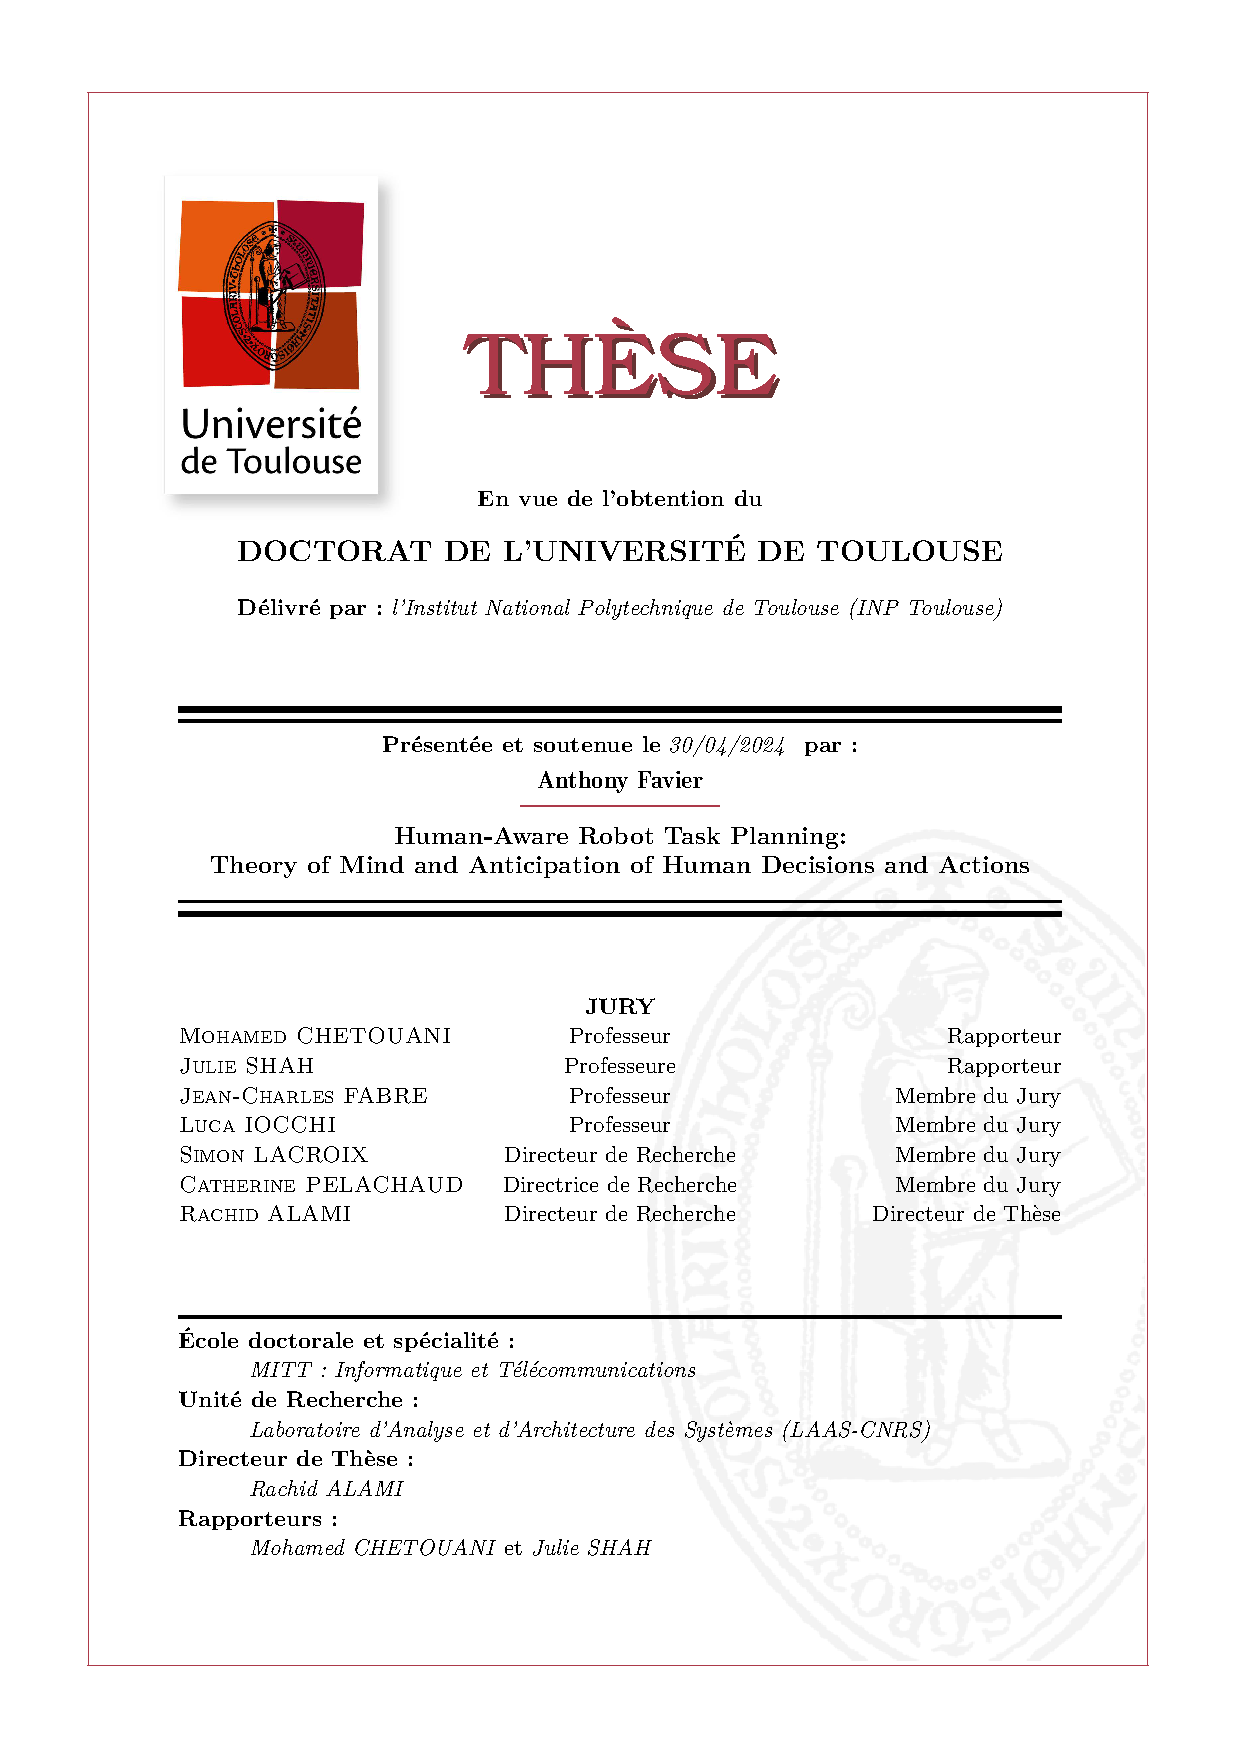
\includepdf[pages=-]{couverture_these_perso.pdf} %
%%%%%%%%%%%%%%% Uncomment this to show custom Cover page %%%%%%%%%


\cleardoublepage %

\dominitoc

\pagenumbering{roman}

\cleardoublepage %

%%%% Acknowledgments %%%%%
%%% Needs an update before and after the defence, write last
\section*{Remerciemments}
 
blabla %

%%%% Abstract %%%%%
\chapter*{Abstract}

% 4000 caractères

Although human-robot collaboration can be beneficial, most of today's robots work in spaces physically separated from humans, or their capabilities are severely limited in close proximity to humans. This work aims to bridge the gap between robotic capabilities and human expectations, fostering a new era of seamless and intuitive collaboration between humans and robots in shared environments to perform industrial, service or domestic tasks. More specifically, this manuscript presents a study of decision-making in the context of human-robot collaboration, particularly in the areas of task planning and simulating intelligent agents.

First, we discuss various fields and works related to human-robot collaboration to better understand my work's context. After an introduction to the HATP/EHDA task planner, I present my first contribution, which incorporates some concepts from the Theory Of Mind into task planning. Some models and algorithms are proposed and evaluated to better estimate and maintain human knowledge during collaboration, in order to better anticipate human behavior. As a result, we can identify when humans have false beliefs about a fact that is evaluated as relevant to the task. In this case, the robot can proactively inform the humans to correct the false information, or the robot can deliberately delay its actions so that the humans can see them. Our results show that this scheme effectively maintains human beliefs and solves a broader class of problems than HATP/EHDA, without communicating systematically.

My second contribution is a new approach to task planning producing a robot behavioral policy ensuring smooth collaboration where the human always has full decision latitude and the robot always conforms in parallel to these decisions. This approach is based on a concurrent and compliant joint action model we have designed. This model, in the form of an automaton, takes into account human uncontrollability and social cues. We also propose a new method of plan evaluation and selection based on the estimation of the human's internal preferences regarding the task. Empirical results show that this approach enables concurrent robot behavior that conforms to human's real-time decisions and preferences.

As another contribution validating the above approach, we implemented our proposed joint action model as an execution scheme into a dedicated simulator. Then, we conducted a user study where participants were invited to collaborate in several scenarios with a simulated robot following policies produced by our approach. In contrast with our approach, we used a baseline where the robot always imposes its decisions on the human. We showed through statistical analysis that our approach satisfies human preferences significantly more successfully than the baseline. Similarly, we have shown that our approach induces significantly more positive interaction, more adaptive and effective collaboration, and significantly more appropriate and accommodating robot decisions.

Finally, my last contributions concern simulating intelligent human agents. Such simulated agents endowed with decision-making capabilities can help to test, evaluate, and robustify interactive and collaborative robot systems. We propose a generic architecture to simulate an intelligent agent and present an implemented version for navigation use cases. An additional contribution capable of simulating several navigating agents is also presented.  
 %
\chapter*{Résumé}

Bien qu'il ait été montré que la collaboration humain-robot puisse être bénéfique, la plupart des robots actuels travaillent dans des espaces physiquement séparés de l'humain ou leurs capacités sont sévèrement limitées à proximité de l'humain. Ce travail vise à combler le fossé entre les capacités robotiques et les attentes humaines, en favorisant une nouvelle ère de collaboration transparente et intuitive entre les humains et les robots dans des environnements partagés pour réaliser à la fois des tâches industrielles, de services ou domestiques. Plus précisément, ce manuscrit présente une étude sur la prise de décision dans le contexte de la collaboration humain-robot, en particulier dans les domaines de la navigation et de la planification des tâches.

Tout d'abord, nous discutons de divers domaines et travaux en lien avec la collaboration humain-robot afin de mieux comprendre le contexte de mon travail. Après une familiarisation avec le planificateur de tâches HATP/EHDA, je présente ma première contribution qui incorpore certains concepts de la théorie de l'esprit dans la planification de tâches. Certains modèles et algorithmes sont proposés et évalués pour mieux estimer et maintenir les connaissances de l'humain lors d'une collaboration afin de mieux anticiper son comportement. En conséquence, nous pouvons identifier quand l'humain a une fausse connaissance d'un fait évalué comme pertinent pour la tâche. Dans ce cas, le robot peut informer l'humain de manière proactive pour corriger la fausse information ou le robot peut retarder volontairement ses actions afin qu'elles soient vu par l'humain. Les résultats montrent que ce schéma permet de maintenir efficacement les connaissances de l'humain et permet de résoudre une classe plus large de problèmes que HATP/EHDA tout en ne communiquant pas systématiquement.

Ma deuxième contribution est une nouvelle approche de planification des tâches produisant une politique comportementale du robot assurant une collaboration fluide où l'humain a toujours une latitude de décision totale et où le robot se conforme toujours en parallèle à ces décisions. Cette approche est basée sur un modèle d'action conjointe simultanée et accommodante que nous avons conçu. Ce modèle, sous la forme d'un automate, tient compte de l'incontrôlabilité de l'humain et des signaux sociaux. Nous proposons également une nouvelle méthode d'évaluation et de sélection des plans basée sur l'estimation des préférences internes de l'humain concernant la tâche. Les résultats empiriques montrent que cette approche permet un comportement concourant du robot qui se conforme aux décisions et aux préférences en temps réel de l'humain.

Pour valider l'approche précédente, nous avons mené une étude utilisateur à l'aide d'un simulateur spécialement développé à cet effet. Les participants ont été invités à collaborer dans plusieurs scénarios avec un robot simulé suivant les politiques produites par notre approche. Nous avons utilisé comme référence une approche opposée à la nôtre dans laquelle l'humain est forcé de se conformer aux choix du robot. Nous avons montré par une analyse statistique que notre approche permettait de satisfaire les préférences des humains de manière nettement plus satisfaisante. De même, nous avons montré que notre approche induit une interaction significativement plus positive, une collaboration plus adaptative et efficace, et des décisions du robot significativement plus adéquates et accommodantes.

Enfin, ma troisième contribution concerne la prise de décision dans le domaine de la navigation. Je propose un système simulant un avatar humain qui, en plus d'être réactif, prend des décisions rationnelles sur les tâches de navigation. Ce système sert d'outil de test et d'évaluation pour les systèmes de navigation robotique. Ainsi, ces derniers peuvent être évalués, ajustés et robustifiés en simulation pour réaliser plus rapidement des expériences matures dans la vie réelle. %

\tableofcontents

% \printnomenclature
\printnoidxglossary[type=\acronymtype]
% \listoffigures
% \listoftables
% Use \mtcfixnomenclature below if you have a glossary (added with
% \printnomenclature above) and you're see a shift in the mini-table of
% contents at the begining of each chapter (example: no mini-toc in chapter 1;
% mini-toc of chapter 1 appearing in chapter 2; and so on).
%
% You should not use \mtcfixnomenclature if you have no glossary (that means,
% if you don't use \printnomenclature or if your glossary is empty).
%\mtcfixnomenclature

\mainmatter
\chapter*{Introduction}
\addstarredchapter{Introduction}
\markboth{Introduction}{Introduction}

\newcommand{\mysection}[1]{%
    \section*{#1}%
    \addcontentsline{toc}{section}{#1}%
    \markright{#1}%
}


\minitoc

\acrfull{hrc} is a growing field in robotics and \acrfull{ai} research that aims to enable safe and effective teamwork between humans and robots.
This field mostly concerns fully autonomous robots. Hence, for instance, it excludes exoskeletons or teleoperated robots such as surgery manipulators or remotely operated (aerial) vehicles. 

In this manuscript, robots are considered autonomous tools able to interact physically with their environment. As tools, robots should facilitate human tasks by reducing both the required physical effort and mental workload. 
Industrial robots are already popular in factories because they are fast, accurate, reliable, and never tire, which makes them ideal for repetitive factory tasks. 
However, such robots are usually contained in dedicated areas where humans cannot enter for safety reasons. 
Hence, it is still an open challenge to endow robots with enough reliable reasoning capabilities and compliant motion control to allow efficient and trusted direct collaboration between humans and robots. 

This work aims to design autonomous robots able to make explainable, acceptable, and efficient decisions to collaborate with humans. Moreover, \acrshort{hrc} can also occur in various contexts that must be taken into account which range from co-worker robots in factories to householder robots for our everyday lives and include service robots in public places like restaurants and shops.


\mysection{Human-Robot Collaboration Challenges}

\acrshort{hrc} opens several challenges to address, each corresponding to a different aspect or functionality that the robot should be endowed with to fulfill its role. Hence, the ideal general collaborative robot should be the aggregation of all the notions below: 

\begin{itemize}
    \item \textbf{Navigation}: The robot should be able to acceptably and efficiently move in a human-populated environment. This implies being mechanically designed for it, anticipating and planning correct trajectories, and being able to adapt and follow these trajectories in real time. The robot should not move threateningly and should account for humans.

    \item \textbf{Manipulation}: The robot should be able to manipulate objects to interact with its environment. Hence, the robot should have an actuator like an arm and a gripper and should be able to exhibit motions that are efficient and safe to nearby humans.

    \item \textbf{Decision-making}: The robot should be able to make relevant decisions to be collaborative. This implies being able to plan its actions to solve a collaborative task. It also implies being able to supervise the task execution and make online decisions to adapt to uncertainties in real time, which includes human actions and commands. 

    \item \textbf{Communication}: To achieve congruent interaction and collaboration, collaborative agents must communicate. This implies that the robot should be able to communicate information to the human and understand the one received from the latter. These communications can be of various types, e.g., verbal, using natural language, prompting text on a screen, and signaling through robot movements (arms, head, mobile base). More innovative techniques can also be mentioned such as projecting arrows or desired paths on the ground, and using Augmented Reality to show internal information on the robot (decision, next action, etc...).

    \item \textbf{Perception}: Eventually, the robot must be able to perceive its environment. This is mandatory for the robot to have a reliable perception scheme to know the position of near objects, obstacles, and humans. First, relevant sensors must be used and placed on the robot or in the environment itself. After, from sensory data, some analysis and reasoning processes must extract relevant facts about the robot's environment such as objects' positions, spatial relations, reachable objects, human knowledge and intentions, the state of the current goal, and more. This constitutes the knowledge of the robot which may include an estimation of the near human knowledge. Perception is critical because most of the other challenges rely on the robot's knowledge.

\end{itemize}
    

\mysection{Contributions and manuscript organization}

The main challenge of HRC/HRI addressed in my PhD is decision-making. My work led to three main contributions concerning two distinguishable subfields. My two first contributions concern decision-making during task planning, to decide and plan the robot's action in order to solve a task collaboratively or simply in the presence of humans. My third contribution addresses decision-making in navigation, especially, how to simulate interactive social navigating agents endowed with decision-making processes to challenge robot navigation schemes.
As a result, the structure of my manuscript is as follows.

Chapter~\ref{chap:1} provides more details about the context of my PhD by discussing related fields and works of HRC. This chapter eventually highlights the gap in the literature that motivates my PhD work.

Part~\ref{part:1} gathers all my work concerning task planning for HRC. It represents a major portion of my PhD work and includes the chapters~\ref{chap:2}, \ref{chap:3}, \ref{chap:4}, \ref{chap:5}, and \ref{chap:6}.

Chapter~\ref{chap:2} familiarizes the reader with the HATP/EHDA task planner. Indeed, I participated in its development and this planner has been the keystone of my two contributions to task-planning for HRC. Hence, the reader should understand both this task planner's motivation and methods.

Chapter~\ref{chap:3} introduces my first main contribution which incorporates Theory of Mind concepts in HRC task-planning, more precisely, in the HATP/EHDA planning process.
Some models and algorithms are proposed and evaluated to better estimate human beliefs in order to better anticipate their potential actions. As a result, we can identify when the human has a false belief about a fact evaluated as relevant for the task. In such cases, the robot can proactively inform the human to correct the false belief or the robot can purposely delay its action to make sure the human sees its execution and infer the corresponding fact, avoiding verbal communication. 

In Chapter~\ref{chap:4}, as my second main contribution, I address the lack of concurrent actions of HATP/EHDA to improve fluency in collaboration. Inspired by the Joint Action literature, we designed a model of concurrent and compliant execution for HRC in the form of an automaton. We also propose to evaluate plans based on an estimation of the human inner preferences. A novel task planning approach taking into account the mentioned execution model and plan evaluation is proposed. This approach generates concurrent robot policies compliant with human online decisions and preferences. 

Chapter~\ref{chap:5} is a technical description of an interactive simulator I developed to execute the robot policy generated by the approach described in the previous chapter. This simulator proposes an execution scheme based on the model of execution to run and supervise the robot policy in a 3D simulator. It also allows a human operator to perform actions through intuitive mouse control. Hence, this simulator offers a way to collaborate with a robot following the approach we designed and is used in the next chapter to evaluate the approach.    

Chapter~\ref{chap:6} presents a user study validating the approach proposed in Chapter~\ref{chap:4} using the simulator described in Chapter~\ref{chap:5}. For this purpose, several scenarios have been designed using a BlocksWorld task, and human participants were asked to collaborate with the simulated robot to evaluate its behavior. We compared our approach with a baseline consisting of a robot following a simpler version of the model of execution. 

Conclusions regarding part~\ref{part:1} follow this chapter before starting the second part of this thesis. 

Part~\ref{part:2} concerns decision-making in navigation and how to simulate interactive social navigating agents. Despite not being my main research topic, this subject represents significant work in my PhD. This part includes the two last chapters: \ref{chap:7} and \ref{chap:8}.

Chapter~\ref{chap:7} describes my third contribution in which I address the decision-making challenge in navigation to allow the robot to move in a human-populated environment acceptably and efficiently. I developed a system producing an ``intelligent'' human avatar that, while being reactive, can make rational decisions about navigation tasks. This system serves as a benchmarking and testing tool for robot navigation systems to be challenged. This way, robot navigation systems can be evaluated, tuned, and stress tested in simulation allowing them to run mature real-life experiments faster.  

Chapter~\ref{chap:8} presents an additional work with the same rationales as the approach described in Chapter~\ref{chap:7} and is largely inspired by it. However, this work addresses a major limitation of the previous one which is not being able to simulate several human agents. This other approach can choreograph several agents with group movements and social behaviors. Despite having limited individual decision-making compared to the previous approach, this additional work generates pertinent and challenging intricate situations with several agents which is beneficial to the social robotic research.

Conclusions concerning both Chapter \ref{chap:7} and \ref{chap:8} end part~\ref{part:2}.

Eventually, I share general conclusions regarding all of my PhD work in a dedicated part before providing additional materials in the appendix.  

\mysection{List of Publications}

\subsubsection*{As main author}
\begin{itemize}

    \item Anthony Favier, Phani-Teja Singamaneni, Rachid Alami. Simulating Intelligent Human Agents for Intricate Social Robot Navigation. Social Robot Navigation workshop - Robotics: Science and Systems (RSS'21), Jul 2021, Washington, United States. 
    \item Anthony Favier, Phani-Teja Singamaneni, Rachid Alami. An Intelligent Human Avatar to Debug and Challenge Human-aware Robot Navigation Systems. Late Breaking Report - 2022 ACM/IEEE International Conference on Human-Robot Interaction (HRI'22), Mar 2022, Sapporo, Japan. 
    \item Anthony Favier, Shashank Shekhar, Rachid Alami. Robust Planning for Human-Robot Joint Tasks with Explicit Reasoning on Human Mental State. AI-HRI Symposium at AAAI Fall Symposium Series (FSS'22), Nov 2022, Arlington, United States. 
    \item Anthony Favier, Shashank Shekhar, Rachid Alami. Anticipating False Beliefs and Planning Pertinent Reactions in Human-Aware Task Planning with Models of Theory of Mind. PlanRob Workshop - International Conference on Automated Planning and Scheduling (ICAPS'23), Jul 2023, Prague, Czech Republic. 
    \item Anthony Favier, Shashank Shekhar, Rachid Alami. Models and Algorithms for Human-Aware Task Planning with Integrated Theory of Mind. IEEE International Conference on Robot and Human Interactive Communication (RO-MAN'23), Aug 2023, Busan, South Korea. 
    \item Anthony Favier, Phani Teja Singamaneni, Rachid Alami. Challenging Human-Aware Robot Navigation with an Intelligent Human Simulation System. Social Simulation Conference (SSC'23), Sep 2023, Glasgow, France. 
    \item Anthony Favier, Rachid Alami. Planning Concurrent Actions and Decisions in Human-Robot Joint Action Context. Symbiotic Society with Avatars workshop - ACM/IEEE International Conference on Human-Robot Interaction (HRI'24), Mar 2024, Boulder, United States.

\end{itemize}
    
\subsubsection*{As co-author}
\begin{itemize}
    
    \item Guilhem Buisan, Anthony Favier, Amandine Mayima, Rachid Alami. HATP/EHDA: A Robot Task Planner Anticipating and Eliciting Human Decisions and Actions. IEEE International Conference On Robotics and Automation (ICRA 2022), May 2022, Philadelphia, United States. ⟨10.1109/ICRA46639.2022.9812227⟩. 
    
    \item Phani-Teja Singamaneni, Anthony Favier, Rachid Alami. Towards Benchmarking Human-Aware Social Robot Navigation: A New Perspective and Metrics. IEEE International Conference on Robot and Human Interactive Communication (RO-MAN), 2023, Aug 2023, Busan, South Korea.
    \item Phani-Teja Singamaneni, Anthony Favier, Rachid Alami. Human-Aware Navigation Planner for Diverse Human-Robot Contexts. 2021 IEEE/RSJ International Conference on Intelligent Robots and Systems (IROS), Sep 2021, Prague (online), Czech Republic. 
    \item Phani-Teja Singamaneni, Anthony Favier, Rachid Alami. Invisible Humans in Human-aware Robot Navigation. IEEE International Conference on Robotics and Automation (ICRA 2022), May 2022, Philadelphia, United States.
    \item Phani-Teja Singamaneni, Anthony Favier, Rachid Alami. Watch out! There may be a Human. Addressing Invisible Humans in Social Navigation. 2022 IEEE/RSJ International Conference on Intelligent Robots and Systems (IROS 2022), Oct 2022, Kyoto, Japan. 

    \item Olivier Hauterville, Camino Fernández, Phani-Teja Singamaneni, Anthony Favier, Vicente Matellán, et al.. IMHuS: Intelligent Multi-Human Simulator. IROS2022 Workshop: Artificial Intelligence for Social Robots Interacting with Humans in the Real World, Oct 2022, Kyoto, Japan. 
    \item Olivier Hauterville, Camino Fernández, Phani-Teja Singamaneni, Anthony Favier, Vicente Matellán, et al.. Interactive Social Agents Simulation Tool for Designing Choreographies for Human-Robot-Interaction Research. ROBOT2022: Fifth Iberian Robotics Conference, Nov 2022, Zaragoza, Spain. 
\end{itemize}
    
    
    
\ifdefined\included
\else
\setcounter{chapter}{0}
\dominitoc
\faketableofcontents
\fi

\chapter{Task Planning for Human Robot Collaboration Context}
\chaptermark{Task Planning for Human Robot Collaboration Context}
\label{chap:1}
\minitoc

\section{Task Planning}

\subsection{Various techniques}
\subsection{Offline}
\subsection{Online}

\section{HRI Interaction}

\subsection{human human interaction}
\subsection{human computer interaction}
\subsection{human robot interaction}

\subsection{navigation}
\subsection{dialogue}


\section{HRC Collaboration}

\subsection{joint action}
\subsection{Whole architecture to work}
\subsection{execution policy, leader follower?}

\section{Background and Our Approach}
\subsection{human-aware task planning state of the art}
\subsection{our Approach}




\part{Human-Aware Task Planning} \label{part:1}
\ifdefined\included
\else
\setcounter{chapter}{1} %% Numéro du chapitre précédent ;)
\dominitoc
\faketableofcontents
\fi

\chapter{A Human-Aware Task Planner Emulating Human Decisions and Actions (HATP/EHDA)}
\chaptermark{HATP/EHDA}
\label{chap:2}
\minitoc

\chapabstract{This chapter presents the HATP/EHDA task planner. This planner has been the keystone of most of my work. Hence, the reader should understand the motivation and methods of this task planner.}

\section{Introduction}

I was introduced to task planning with the work of a PhD student from my lab, Guilhem Buisan. I slightly contributed to the original version and then proposed two extensions of his work. However, Guilhem mainly designed and implemented this novel \textbf{H}uman-\textbf{A}ware \textbf{T}ask \textbf{P}lanning approach dedicated to \acrfull{hri}, which plans the robot's actions while estimating and \textbf{E}mulating the \textbf{H}uman \textbf{D}ecisions and \textbf{A}ctions, namely \textbf{HATP/EHDA}. 

We believe this planning approach suits the needs of \acrshort{hri} scenarios well; thus, it became a laboratory to address relevant challenges of task planning for \acrshort{hrc}. 
Two of my main contributions include addressing such challenges and implementing the solutions as extensions of HATP/EHDA.   
Consequently, it is essential to understand this work's motivation and methods well before introducing my proper contributions. This section introduces, motivates, and explains the HATP/EHDA approach as a background to the other chapters. 
A detailed description of this prototypical planner is already given in Buisan's thesis~\cite{thesisBuisan21}. Thus, large parts of this section are directly retrieved from Buisan's thesis, but they are essential to have in mind. Some notations are adapted to match the descriptions of my contributions in the following chapters. 

\section{A Hierarchical Agent-Based Task Planner (HATP)}

My work and HATP/EHDA are part of a line of work that started with the \acrfull{hatp} \cite{alili2009task,lallement2014hatp}.

Based on \acrfull{htn}, this planner can elaborate a multi-agent plan based on a single HTN tree. Moreover, it maintains one belief base per agent, allowing the writer to write task decomposition rules and action preconditions and effects in any agent belief base. This approach produces a joint plan that includes actions from all involved agents. 

Finally, to make \acrshort{hatp} suitable to \acrshort{hri} scenarios, specific mechanisms to compute costs and filter plans have been included. To this end, \acrshort{hatp} allows balancing efficiency, wasted time, agent effort, intricacy, and undesirable states or sequences. This way, social rules can be defined to produce a collaborative plan that humans will likely accept. 

However, \acrshort{hatp} assumes a shared goal has been established between humans and robots before planning. The generated plan will be shared with and accepted by humans before execution. Indeed, HATP does not represent humans as agents having separate decision-making processes that may lead to diverging plans without robot communication. Hence, any human deviation from their generated stream of action needs supervision to perform repair action or request a replanning. Such an approach can work well, but it assumes that communication can easily be done at any point in the plan. However, this assumption is not always verified for various reasons, \textit{e.g.} noisy environments, making communication costly.
Additionally, any human deviation, \textit{e.g.} due to inattention, will put the robot in a failure state, which needs to be fixed before continuing (replanning).

\section{Rationales of the HATP/EHDA Approach}

The \acrshort{hatp} approach produces what is estimated to be the best joint plan for solving the task. Hence, this approach assumes that humans will likely accept and follow the produced plan. This approach leaves no room for online human decisions and assumes a fully committed human through a previously established shared goal. This approach also considers one shared task representation and knowledge base. To cater to the limitations of \acrshort{hatp}, I participated in the development of a new approach, HATP/EHDA, which tries to satisfy several objectives: 
\begin{enumerate}
    \item \textbf{Plan without assuming a prior shared goal.} In \acrshort{hri} scenarios, the robot and the human do not always share a goal. The robot can, for example, plan to perform a task around humans that are not involved at first, or it may be requested by a human to do a task without wanting to take part in it. HATP/EHDA can balance between integrating the sharing of a goal with a human (assumed to be collaborative) in the plan and making the robot do the task alone or integrating the eventuality to ask for punctual human help. 

    \item \textbf{Model the human decision processes.} When taking part in a task, a human (assumed willing to collaborate with the robot) will also plan to reach their (potentially shared) goal. HATP/EHDA must be able to account for this to provide plans that are expected and explainable by the human partner.

    \item \textbf{Help the human decisions, but not compel them.} Unlike \acrshort{hatp}, HATP/EHDA should account for human decision-making flexibility. While modeling the human decision processes, it is possible to narrow down the possible human actions, and the generated plans must help the supervision (execution of the plan) avoid replanning or repairing during the execution by considering several human actions.

    \item \textbf{Model the potential human reactions.} It is possible to predict that the human may react to some situations, interrupting or helping their current task. Two causes have been identified for these reactions. First, they can result from specific world states humans perceive and interpret. Then, they can also originate from explicit communications issued by the robot. These communications can either be a belief alignment, updating the human knowledge and impacting their decisions, a request to perform a specific action, or a request to help the robot with a shared goal, needing the human to plan for it.

    \item \textbf{Act and decide on the different agents' beliefs.} It is crucial to be able to represent actions as having different effects on the beliefs of the robot or the human. Indeed, some robot actions are partially or not observable by humans; humans cannot know the complete new world state when performing them. Besides, these effects and their observability often depend on the current world state, whose representation must be supported by the planner. Then, planning decisions may require reasoning on both the robot's and human's beliefs. This is especially true with communication actions aiming to align knowledge or ask questions. Finally, some actions of pure decision have no direct effect on the world but only on the internal beliefs of the agents. For example, observation actions will only update the beliefs of the agent doing it.

    \item \textbf{Decide not only on the world state but also on the decision processes of the agents.} Some decisions made during the planning process require access to the agents' beliefs representing the world state and the estimation of their planning processes. For example, the decomposition of a task by the robot may be impossible if some other task is already performed in its partial plan. Other decisions may also need the estimation of the current human planning process. For example, if it were estimated earlier in the plan that the human would perform a specific task decomposition, the planner would assign a complementary task to the robot.

    \item \textbf{Adapt to the human experience, trust, and preferences.} We also want the planning process to be adjusted depending on the actual human it is planning with. It must perform its planned search differently, whether the human has the habit of performing this particular task with the robot or not. Moreover, the human model can be adjusted to the human's trust in the robot and their preferences.

\end{enumerate}

\section{Related work} \label{sec:ch2_related_work}

An approach to solving a collaborative task is to produce a joint plan that includes coordinated robot and human actions. This plan must be shared, accepted, and followed to solve collaboratively the common goal. This approach is used in the \acrshort{hatp} planner presented above. By assuming the plan must be followed, the human cannot deviate from the generated plan. Hence, this approach assumes that the human is controllable. 
In \cite{johannsmeier2016hierarchical}, the authors use the same assumption and propose a task allocation framework for human-robot collaborative assembly line tasks. They propose representing the task through an AND/OR graph and solving the optimal sub-task allocation problem considering a given cost function. Action sequences are extracted from this allocation and then shared with the respective agents to be executed. Hierarchical and concurrent hybrid state machines handle the execution of these sequences. This copes with unpredictable events likely to happen in dynamic and partially known environments, especially in the presence of humans.  

Additionally, some works are focused on \acrshort{hrc}'s psychological aspect, like the plan's acceptability and explainability. This is beneficial to the approach described just above. In \cite{chakraborti_plan_2017}, the authors propose to improve the explainability of a robot plan by using both a robot model $\mathcal{M^R}$ and the estimation of the model the human has of it $\mathcal{M}^R_h$. This approach, called model reconciliation, aims to make identical the optimal plans generated using both models, i.e., $\mathcal{M^R}$ and $\mathcal{M^R_h}$. They define a list of operators to modify the different models until the plans match. 
Although this approach interestingly improves the explainability of the robot's plan, it does not consider the two agents to collaborate directly. Indeed, the plan produced only contains robot actions. 

Producing a joint plan that considers the human controllable is efficient and acceptable in industrial contexts. Indeed, the human is working and thus highly committed and focused on the task. Even if humans appreciate flexibility, in this context, their priority is instead task efficiency.
However, this assumption can become burdensome for humans in other contexts, such as household ones, where humans are likely to be distracted, change their minds, and tend to prioritize minimizing their effort and flexibility instead of task efficiency. 

As a result, some approaches started to consider a distinct human model $\mathcal{M}^R_h$ to plan the robot action.
A first approach, described in \cite{hoffman_effects_2007}, proposes an adaptive action selection mechanism for a robotic teammate, making anticipatory decisions based on the confidence of their validity and their relative risk. They demonstrate improved task efficiency and fluency compared to a purely reactive process. The human behavior is modeled with a First-Order Markov Process and learned through Bayesian estimate. The probabilities constituting the human model are used in the cost evaluation of different plans, eventually leading to a robot action selection, producing an adaptive and proactive robot plan. 
In \cite{unhelkar2020decision} is proposed an approach based on \acrfull{pomdp} called CommPlan. The \acrshort{pomdp} is built using a user-defined \acrfull{mdp} representing the collaborative task and an \acrfull{amm} representing the human decision-making process. Solving this \acrshort{pomdp} produces a robot policy that decides when the robot has to communicate about its beliefs, when to question the human about theirs, and when to ask the human to perform an action. Besides, the \acrshort{amm} is not only specified by an expert modeler but also refined during the interaction via learning. However, the approach considers the human model as an oracle on which reasoning is hardly possible.

Other works extend the use of a distinct human model to explicitly predict and anticipate the actions the human is likely to perform. Then, for each possible human action, the best robot's actions are determined to account for human unpredictability. This is the approach used in HATP/EHDA.
This other work \cite{buckingham_robot_2020} also uses this approach. They propose a unified scheme to cope with collaborative, adversarial, and non-involved human agents. This scheme considers given mental models for each human co-present with the robot, which might interact with the latter. These mental models are queried to estimate a set of actions each agent is likely to perform given a state. The robot's actions are planned according to these estimated actions to reach the robot's goal and potentially achieve the human agents' goal. In doing so, the robot's actions can influence the human ones without explicit communication, helping the robot achieve its goal. HATP/EHDA similarly queries a human mental model and uses an AND/OR graph where OR nodes represent possible robot actions in a state and AND nodes represent the possible human actions estimated by the models. However, despite saying the model can be generic, this work uses a basic breadth-first search planner to produce a set of minimal-cost plans solving the estimated human goal. Then, they extract the first actions of each plan to produce a set of actions the human is likely to perform. No details are given on the cost evaluation. This approach does not seem to consider human actions that are sub-optimal but still probable, which can be due to inattention. Moreover, the robot actions are selected by using a Min-Max approach on the AND/OR graph, minimizing the worst-case. This approach works well in adversarial setups and still allows cooperative human interventions. However, it is unclear how these cooperative actions are taken into account in the robot decision process. Assuming that the human will be adversarial, the robot might make ``wrong'' decisions, possibly preventing an efficient and optimal cooperative execution. HATP/EHDA minimizes the average cost of all possible human decisions, optimizing uniformly for any human decisions. This approach considers humans congruent, rational, and cooperative but not necessarily involved in the robot's task. Hence, HATP/EHDA does not account for adversarial humans but addresses the other cooperation types better.
\cite{koppula2016anticipatory} also explicitly estimated the most likely human actions to generate the robot policy, but they use a probabilistic and learning approach. They propose a two agent collaborative \acrshort{mdp} model and learn robot policies by taking into account the actions that can be performed by the human. They represent the environment in terms of the object affordances and learn the activity model from RGB-D videos of a human performing the activities. Then, they use this learned task model in a distributed Q-learning algorithm to learn the robot policy for a given new environment. 
The human capabilities are captured in a \acrshort{mdp}. Thus, the possible human actions are estimated by balancing the human habits and the best ($\epsilon$-optimal) action given by the \acrshort{mdp}. 


Another line of work, sometimes also using human models, is focused on online and reactive planning. The robot's behavior is decided online using planning techniques but on limited horizons. This produces robot behaviors that are adaptive to human decisions and potentially unexpected environmental changes and events. However, due to the limited horizon to maintain a real-time reactive behavior, the robot behavior's optimality is not guaranteed and might lead to dead ends. Nevertheless, these online approaches usually robustify the robot's behavior and are reactive to failures. Therefore, they could/should complement offline planning approaches like HATP/EHDA.
The two-sided work \cite{sanelli_short_term_2017} is in this line of work. First, they propose a conditional planning system that considers uncertainties, primarily due to human agents. This planning approach is based on planner Contingent-FF \cite{hoffmann2005contingent}. Then, they propose a component to translate these plans into a Robust Petri-Net Plan (PNP) to handle their execution. This translation is inspired by work \cite{iocchi2016practical}, which improves plans with execution rules. Eventually, these plans are executed with an existing module called PNPRos \cite{ziparo2011petri}. Interestingly, the expected human actions are transformed into sub-Petri Nets where the robot elicits the action (\textit{e.g.}, via verbal communication) if the human does not perform it by themselves. 
However, this approach does not model either reason on a distinct human agent model. Hence, the human reasoning process, goal, and belief are not modeled. This means that the interaction is limited to requesting the human to perform single actions without setting a proper high-level joint goal. This can be efficient in some situations, like a service robot providing information and requesting answers to some questions, such as the examples presented by the authors. However, repeated punctual interventions to perform a more extended task collaboratively can become unpleasant for the human.
In \cite{DarvishSMC21}, they propose a hierarchical human-robot cooperation architecture called FlexHRC+ designed to provide collaborative robots with an extended degree of autonomy when supporting human operators in high-variability shop-floor tasks. This online architecture is organized into three levels: perception, representation, and action, producing robust, adaptive, and sometimes proactive collaboration. 
They use hierarchical AND/OR graphs where arcs are sub AND/OR graphs to reduce the complexity of task descriptions, especially when including repetitive subsequences of action (like mounting four table legs). This representation is close to the \acrshort{htn} one used in HATP/EHDA. 
A reactive human-aware task planner is proposed in \cite{fusaro_human_aware_2021}, taking advantage of the Behavior Tree paradigm. The approach plans the robot's actions online by minimizing weighted costs based on duration, ergonomics, and distance, which are updated online. Therefore, the robot can adapt to dynamic changes in the environment and to human intentions, motions, decisions, and availability. This approach permits considering different levels of engagement between robots and humans: coexistence, cooperation, and autonomous task execution. 

Finally, in \cite{izquierdo_badiola_improved_2022}, the authors combine the production of a joint plan to solve a common goal with the reactive aspect of previous approaches. 
They use a so-called ``\textit{agent state}'' to model the human mental state and translate it into action costs in a PDDL domain. This model comprises the \textit{Capacity} evaluating if the human is capable of performing an action at the specified location without difficulty, the \textit{Knowledge} evaluating if the human has all necessary knowledge to perform their assigned actions, and the \textit{Motivation} indicating if the agent is committed towards the common goal, active and not distracted. 
In their approach, the \textit{agent state} is sensed and updated during execution. Then, whenever changes in the \textit{agent state} are detected, a replan is triggered to consider those changes in the plan, often inducing a reassignment of the actions and avoiding the probable failure of the initial plan. However, the authors do not provide a method to effectively sense and estimate the \textit{agent state} but prove its usefulness by simulating its acquisition.


\section{Running Example}

\begin{figure}
    \centering
    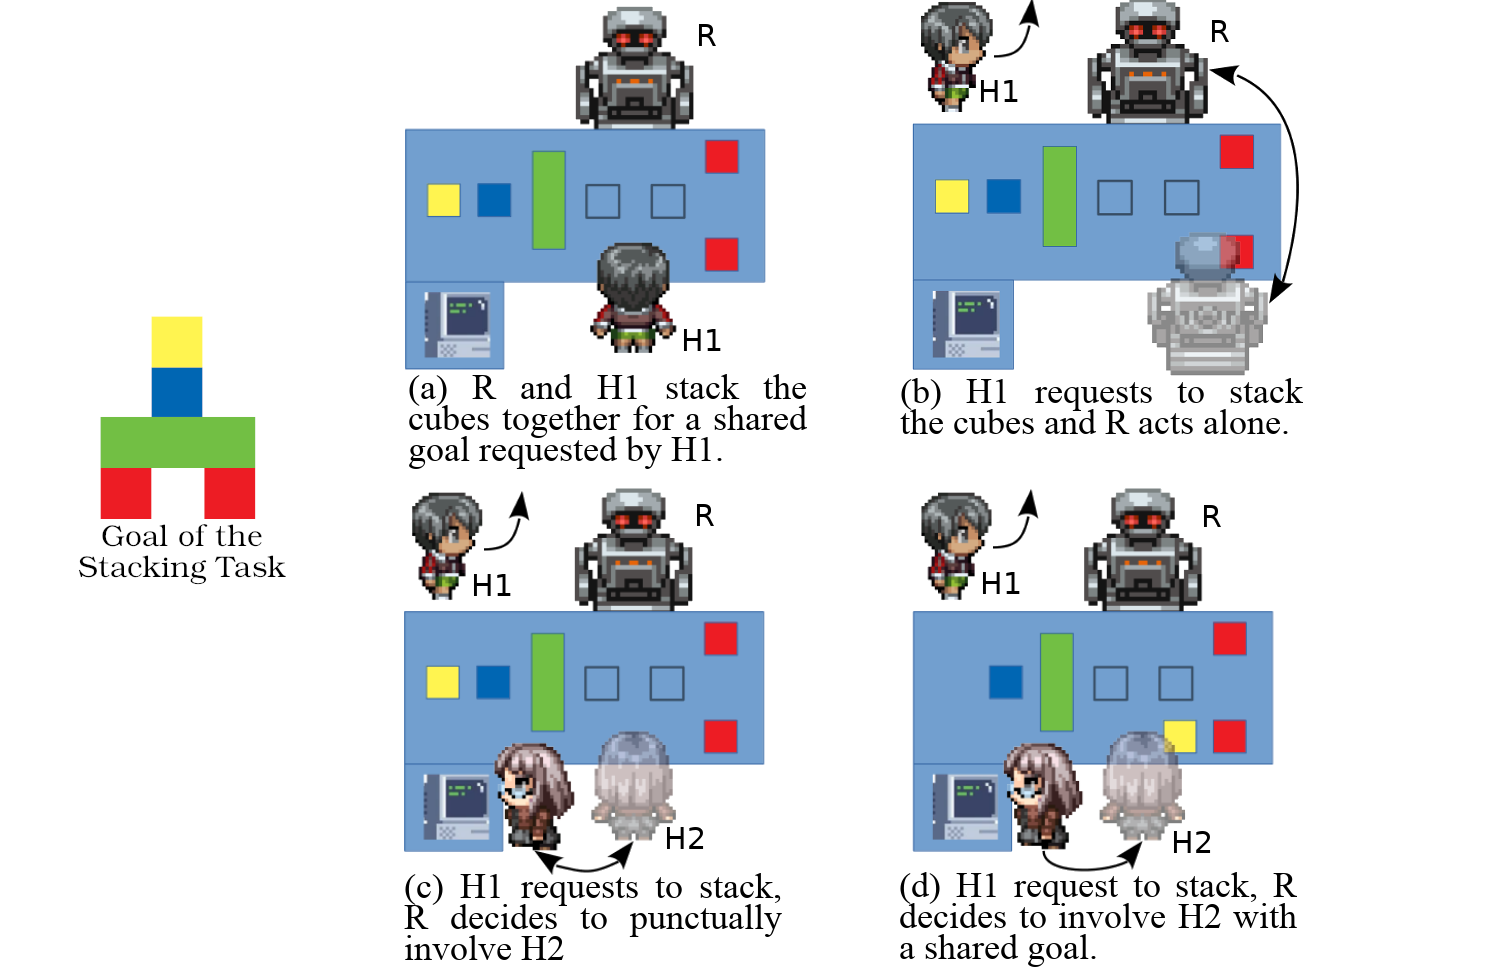
\includegraphics[width=\linewidth]{Chapter2/scenarios.png}
    \caption{Cube stacking scene: A different plan is selected for each scenario, involving nearby humans in the least disturbing way possible}.
    \label{fig:scenarios}
\end{figure}

To highlight the potential of our approach, we present a cube-stacking scene as an example. The scene is depicted in four different scenarios in \ref{fig:scenarios}. The goal consists of stacking the colored cubes on the empty marks to match the colors on the figure's left. All cubes placed in the middle of the table are reachable from anywhere. However, when close to one side, a cube is only reachable from this specific side. Notice that one of the required red cubes is located on the opposite side of the table and cannot be grabbed by the robot in the initial state.

A first human, called \textit{H1}, requests the robot to stack the colored cubes to match the goal pattern given. In the first case (a), \textit{H1} set a shared collaboration goal by requesting the robot to stack the cubes together with them. However, \textit{H1} can also just give their request to the robot and leave. In such a case, the robot has three possibilities. First, in (b), the robot can solve the task alone but must move to the other side of the table, which is slow and costly. Secondly, in (c), the robot can ask another nearby human, \textit{H2}, for punctual help with the unreachable red cube. \textit{H2}'s reaction can be to put the red cube directly in the stack or only make it reachable to the robot. Finally, the robot can set a shared goal by requesting \textit{H2} to help it build the stack together. 

The HATP/EHDA approach explores and evaluates all these kinds of scenarios to produce the robot policy.


\section{Formalization}

This section describes the formalization introduced by the HATP/EHDA planning approach and used or adapted in my contributions. It includes descriptions of the problem specifications and the solution produced by the planner.  

\subsection*{Problem Specification}
\label{sec:problem_spec}

The notations from Buisan's thesis have been adapted to match the notations in this thesis and ease readers' comprehension. We start from the classical planning formalization described in~\cite{ghallab2016automated}.

\begin{definition}
    \textbf{(Classical Planning Domain $\Sigma$.)} A \emph{classical planning domain} is a state-transition system in the following form: $\Sigma = (S, A,\gamma)$. $S$ is a finite set of \emph{states} in which the system may be, $A$ is a finite set of \emph{actions} that the agents may perform, $\gamma: S \times A \rightarrow S$ is a \emph{state-transition function}. Each \emph{state} $s \in S$ is a description of the properties of various objects in the planner's environment. 
    \label{def:classical_planning_domain}
\end{definition}

To represent the objects and their properties, we will use two sets $B$ and $X$: $B$ is a set of names for all the objects, plus any mathematical constants representing the properties of those objects. $X$ is a set of syntactic terms called state variables, s.t. the value of each $x \in X$ depends solely on the state $s$.

\begin{definition}
    \textbf{(State-variable $x$.)} A \emph{state-variable} over $B$ is a syntactic term $x = sv(b_1, ..., b_k)$, where $sv$ is a symbol called the state variable's name, and each $b_i$ is a member of $B$ and a parameter of $x$. Each \emph{state-variable} $x$ has a range, $\textit{Range}(x) \subseteq B$, which is the set of all possible values for $x$.
    \label{def:state_variable}
\end{definition}



Here is the description of the sets $B$ and $X$ for the stacking example given in the introduction:
{\small
\begin{align*}
&B           = Entities \cup Locations \cup Reachability \cup Booleans \cup \{\textsf{nil}\} \\
&\quad Entities    = Agents \cup Cubes\\
&\quad Agents      = \{ \textsf{R}, \textsf{H} \} ~~ \backslash\backslash~\textsf{R}:robot,~\textsf{H}:human\\
&\quad Cubes     = \{ \textsf{red1}, \textsf{red2}, \textsf{green1}, \textsf{blue1}, \textsf{yellow1} \}\\
&\quad Locations     = \{ \textsf{base1}, \textsf{base2}, \textsf{bridge}, \textsf{top1}, \textsf{top2} \}\\
&\quad Reachability     = \{ \textsf{middle}, \textsf{side\_h}, \textsf{side\_r} \}\\
&\quad Booleans    = \{ \textsf{true},\textsf{false} \}\\
&\\
&X = \{ at(e), holding(a), solution(l) ~ | ~ e \in Entities, \varphi \in Agents, l \in StackLocations\}\\
&\quad \textit{Range}(holding(\varphi) ~|~ \varphi \in Agents) = Cubes \cup \{\textsf{nil}\} \\
&\quad \textit{Range}(at(\varphi) ~|~ \varphi \in Agents) = \{ \textsf{side\_h}, \textsf{side\_r} \}\\
&\quad \textit{Range}(at(c) ~|~ c \in Cubes) = Reachability \cup Locations\\
&\quad \textit{Range}(solution(l) ~|~ l \in StackLocations) = Cubes \\
\end{align*}
}

% \vspace{-1cm}


\begin{definition}
    \textbf{(Variable value assignment function $val$.)} A \emph{variable value assignment function} over $X$ is a function $val$ that maps each $x_i \in X$ into a value $z_i \in$ $\textit{Range}(x_i)$. With $X = \{ x_1, ..., x_n \}$, this function can be written as a set of assertions: $val = \{ x_1=z_1, \ldots, x_n=z_n \}$. 
    \label{def:variable_value_assignment_function}
\end{definition}


\begin{definition}
    \textbf{(Action $a$.)} An \emph{action} is a tuple $a = (\textit{head}(a), \textit{pre}(a), \textit{eff}(a))$ where $\textit{head}(a)$ is a syntactic expression of the form $\textit{act}(z_1, ..., z_k)$ where $act$ is a symbol called the \emph{action name} and $z_1,...,z_k$ are variables called parameters. $\textit{pre}(a) = \{ p_1, ..., p_m \}$ is a set of preconditions, each of which is a literal. And $\textit{eff}(a) = \{ e_1, ..., e_n \}$ is a set of effects, each of which is an expression of the form: $sv(t_1, ..., t_j) \leftarrow t_0$ with $t_0$ being the value to assign to the state variable $sv(t_1, ..., t_j)$. We note $\textit{agt}(a)$ the agent performing the action $a$.
    \label{def:action}
\end{definition}


The problem specification of HATP/EHDA is a pair of two distinct human and robot models as follows: $\mathcal{P} = \{ \mathcal{M}^H, \mathcal{M}^R \}$. Each model $\mathcal{M}^\varphi$, for an agent $\varphi$, comprises the following:
\begin{itemize}
    \item \textbf{Name} ($name^{\varphi}$): being the name of the agent. Hence, either ``robot'' or ``human''.
    
    \item \textbf{Beliefs} ($val^{\varphi}$): estimation of the world state from the agent's perspective.
    
    \item \textbf{Agenda} ($d^{\varphi}$): capturing the personal and/or shared goals of the agent, currently implemented as a task list/sequence but could be generalized to partially ordered task networks.
    
    \item \textbf{Partial Plan} ($\pi^{\varphi}$): storing the current partial plan on an agent. This is empty at the beginning and filled during the planning process.
    
    \item \textbf{Action Model} ($\Lambda^{\varphi}$): encoding the capabilities of the agent and used to estimate the next actions of the agent given a goal and a world state. Here, it is described by a \acrfull{htn} and thus a set of operators and methods. 
    
    \item \textbf{Triggers} ($Tr^{\varphi}$): describes the reactions the agent may have which might update their agenda. The agent may react to a specific world state, event sequence, or explicit communication. For instance, consider a scenario where another agent is suddenly handing over an object to the agent. This event has nothing to do with the agent's goal, and thus, the next agent action extracted from the Action Model might not consider the other agent. However, a natural reaction to this situation is to grab the handed object. Thanks to the Triggers mechanic, we can model and predict that whatever the agent is doing, the agent will grab the object when given.  
\end{itemize}

Note that most of the models' elements are static during the planning process. Only the Beliefs ($val^{\varphi}$), the Agenda ($d^{\varphi}$) and the Partial Plan ($\pi^{\varphi}$) of each agent evolve during the planning process. 
That is why we define specifically an \textbf{agent state} in Definition~\ref{def:agent_state}.

\begin{definition}
    \textbf{(Agent state $\sigma$.)} An \emph{agent state} $\sigma^{\varphi}$ comprises the dynamic information evolving during the planning process about an agent $\varphi$. It consists of the agent's beliefs, agenda, and partial plan. Hence, the \emph{agent state} is written as follows: $\sigma^{\varphi} = \{ val^{\varphi}, d^{\varphi}, \pi^{\varphi} \}$.
    \label{def:agent_state}
\end{definition}

\begin{definition}
    \textbf{(Agent model $\mathcal{M}$.)} An \emph{agent model} $\mathcal{M}^{\varphi}$ comprises all information regarding an agent $\varphi$. It consists of the static information, such as the agent's name, action model, and triggers, and the dynamic information gathered in the \emph{agent state}. Hence,  an \emph{agent model} is formalized as $\mathcal{M}^{\varphi} = \{ name^{\varphi}, \sigma^{\varphi}, \Lambda^{\varphi}, Tr^{\varphi} \}$.
    \label{def:agent_model}
\end{definition}

The planner uses two agent models, one for the human and one for the robot. Despite their identical structure, the two models have a fundamental difference: one is a controllable agent and not the other. Indeed, the human model is only used to speculate on human decisions and actions in given situations. 
Then, the robot model is used to plan the robot's actions according to the estimated human actions.
Note that human decisions can still be influenced by the robot's actions, but they cannot be compelled.
It is also important to remember that the two agents are not equivalent. The robot's role is to help, assist, and facilitate humans. Therefore, it should exhibit pertinent, legible, and acceptable behavior.

\begin{definition}
    \textbf{(State $s$.)} A \emph{state} $s_i \in S$ is a tuple composed of two \emph{agent states} capturing the state in which the planning problem is, s.t. $s_i = ( \sigma^{H}_i, \sigma^{R}_i )$.
    \label{def:state}
\end{definition}
 

From the robot's perspective, the state of the world is captured by the variable value assignment function $val^R_i \in \sigma^{R}_i$. Since the planner is assumed to be part of the robot, the robot's beliefs are assumed to be the ground truth and are sometimes noted as $val_i$. 
Similarly, $val^H_i \in \sigma^{H}_i$ represents the estimation of $val_i$ from the human's perspective, also called the estimated human beliefs. 
Therefore, we can define estimated human \textbf{false belief} in Definition~\ref{def:false_belief}.

\begin{definition}
    \textbf{(False belief.)} We say that a state $s_i \in S$ contains \emph{false beliefs}, or \emph{belief divergences}, if $\exists x_j \in X, val^H_i(x_j) \neq val^R_i(x_j)$. 
    \label{def:false_belief}
\end{definition}


Be careful not to confuse \textbf{\textit{states}} and \textbf{\textit{beliefs}}. A \textit{state} is a state in which a given planning problem is. It comprises the robot and human \textit{agent states}. Each \textit{state} is connected to another through agent actions. On the other hand, the \textit{beliefs} refer to the state of the world from an agent's perspective. Both human and robot \textit{beliefs} are part of a \textit{state}.



As an example, considering the presented stacking example, the associated initial state $s_0$ would be as follows: 

{\small
\begin{align*}
&s_0 = \{\sigma^R_0, \sigma^H_0\} \\
&\quad \sigma^R_0 = \{ val^R_0, d^R_0, \pi^R_0 \}, \quad \sigma^H_0 = \{ val^H_0, d^H_0, \pi^H_0 \} \\
&\quad d^R_0 = \{ Stack \}, \quad d^H_0 = \{  \} \\
&\quad \pi^R_0 = \pi^H_0 = \{  \} \\
&\quad val^R_0 = val^H_0 = \{at(\textsf{R}) = \textsf{side\_r},~at(\textsf{H}) = \textsf{side\_h}, ~at(\textsf{red1}) = \textsf{side\_r}, \\
&\quad \quad \quad at(\textsf{red2}) = \textsf{side\_h}, ~at(c) = \textsf{middle} ~|~ c \in Cubes\backslash\{ \textsf{red1}, \textsf{red2} \}, \\
&\quad \quad \quad holding(\textsf{R}) = holding(\textsf{H}) = \textsf{nil}, \\
&\quad \quad \quad solution(\textsf{base1}) = \textsf{red}, ~solution(\textsf{base2} = \textsf{red}), ~solution(\textsf{bridge} = \textsf{green}),   \\
&\quad \quad \quad solution(\textsf{top1}) = \textsf{blue}, ~solution(\textsf{top2} = \textsf{yellow}) \}  \\
\end{align*}
}

Note that our model permits interaction with only one human at a time. Hence, in scenario (a) on figure~\ref{fig:scenarios}, $\mathcal{M}^H$ corresponds to \textit{H1}. In all other scenarios, it corresponds to \textit{H2}.
Therefore, $d^H_0$ is empty except in scenario (a), where \textit{H1} establishes a shared goal. Also, the sets $B$ and $X$ have been slightly modified for legibility reasons because the cubes are, in fact, explicitly associated with colors used in the task decompositions. As a result, the solution is expressed using colors and not the cube names. Finding the exact cube to place is described in the action models.

\subsection*{Planning and Estimating Actions}

As mentioned above, the two models $\mathcal{M}^R$ and $\mathcal{M}^H$ are fundamentally different. The human one is used to estimate the actions that the human is likely to perform in a given situation. The robot one is used to plan the best robot actions according to the estimated human ones. Nevertheless, to simplify the description, we tend to refer to both cases as ``estimating an agent's next actions''.

The exact process of estimating the next actions that an agent $\varphi \in Agents$ is likely to perform in a state $s_i \in S$ will be detailed later. Here, we only consider an overview to introduce some notations. 
The process roughly consists of using the agent's static action model ($\Lambda^{\varphi}$) 
and the dynamic agent's beliefs ($\valf[\varphi][i]$)
to refine the agent's agenda ($\agenda[\varphi][i]$). This refining process returns a so-class \textit{refinement} defined in Definition~\ref{def:refinement}.
%  s.t. $ref(\agenda[\varphi][i], \valf[\varphi][i]) = \{ (a_1,\agenda[][]1), ..., (a_k,\agenda[][]k) \}$ 

\begin{definition}
    \textbf{(Refinement $ref$.)} A \emph{refinement} is a list of 2-tuples for each estimated action, $a$, and the associated new agenda, $d$, after being refined, s.t., $ref(\agenda[\varphi][i], \valf[\varphi][i]) = \{ (a_1,\agenda[][]1), ..., (a_k,\agenda[][]k) \}$. It is computed using the agent's action model $\Lambda^{\varphi}$.
    \label{def:refinement}
\end{definition}

 %%%%%%%%%%%%%%%%%%%%%%%%%%%%

% Estimating the next actions that an agent $\varphi \in Agents$ is likely to perform in a state $s_i \in S$ will be detailed later. Meanwhile, when refining the agent's agenda $d^{\varphi}$ based on its belief $val^\varphi_i$, we obtain a \textit{refinement} as follows $\textit{ref}(d^\varphi_i, val^\varphi_i)= \{ (a_1,d_1),...,(a_j,d_j) \}$. 
% A \textit{refinement} contains a tuple for each estimated possible action $a_j$ and the associated new agenda $d_j$ after being refined. 

In our cooking example, we obtain the following refinement if the starting agent is the human:

\begin{equation*}
    ref(d^H_0, val^H_0) = \{ (add\_salt(),d_1), (move\_to(\textsf{kitchen}),d_2) \}
\end{equation*}

The execution of an action $a$ in HATP/EHDA is seen and known by both agents. Thus, $\forall \varphi \in Agents, \forall x \in X$: 
\begin{equation*}
    \valf[\varphi][i+1](x) = \left\{ 
    \begin{array}{ll}
        w, & \mbox{if} ~ x \leftarrow w \in \textit{eff}(a)   \\ 
        val_i(x), & \mbox{otherwise}
    \end{array}\right.
\end{equation*}


\subsection*{Solution description}

HATP/EHDA produces a robot policy extracted from an implicitly coordinated joint solution tree. This solution tree is an AND/OR tree where AND nodes correspond to human decisions, all possible human choices are preserved, and each OR node corresponds to a robot action selected among the possible robot actions. This representation assumes a turn-taking fashion where agents act one after another alternatively. The solution is formally defined in definition~\ref{def:joint-sol-plan}.

\begin{definition} 
    \label{def:joint-sol-plan}
    \textbf{(Implicitly Coordinated Joint Solution.)} 
    {The solution for $P$ is represented as a tree, i.e. $G=(V,E)$. Each vertex ($v \in V$) represents the robot's belief state, starting from the initial belief. Each edge ($e \in E$) represents a primitive task that is either a robot's action $a^{r}$ or a human's estimated and emulated action $a^{h}$. $G$ gets branched on the possible choices ($a^{h}_1$, $a^{h}_2$, ..., $a^{h}_m$). 
    }  
    \end{definition}
    
In practice, it produces a tree of sequential actions where every human action is succeeded by one optimal robot action. Additionally, a new branch is created for every estimated possible human action, ensuring it covers all possible human choices. Each branch is a possible course of alternating robot and human actions leading to the goal.
Each branch in the solution tree is a sequence of primitive actions, say $\pi=(a_1^h,a_2^r,a_3^h,...,a_{k-1}^h,a_k^r)$, that must satisfy all the solution conditions of $^mathcal{P}$. 
Here, each $a_i^h$ represents a choice, often out of several, the human could make. And each $a_{i+1}^r$ is the optimal robot action according to $a_i^h$.


\section{Exploration}

To start planning, HATP/EHDA must be given the two action models (the robot and the human HTNs), the initial beliefs of both agents (which can differ), and the initial agenda of both agents. The initial agenda of the robot represents the task to decompose, while the agenda of the human represents any task the human is estimated to be committed to. If a shared goal has been established prior to planning between the robot and the human (\textit{e.g.}, the human asking to perform a task with the robot), the agenda of both agents will be filled with the same task.

The planning process is done in three parts: (1) both HTNs are explored in a turn-taking fashion, resulting in a valid joint plans tree; (2) based on this tree, robot actions are selected according to action, plan-wide and social costs, resulting in a conditional plan, where at each step multiple human actions can be performed but only one robot action is set; (3) causal and threat links are added between actions of the conditional plan to ease its execution.

The robot HTN exploration is a pretty standard depth-first algorithm. The first task $\lambda$ from its agenda $d^R$ is popped, then if it is an abstract task $\lambda \in Ab$, all the applicable methods are applied, and their results are prepended to the agenda, thus giving new agents state (with the same beliefs as the previous ones but with the robot agenda updated) and branching our search space. We recursively iterate with the new task popped from the new robot agenda. Eventually, the popped task will be a primitive one $\lambda \in Op$, and its function will be applied to the currently explored agent states. If it returns \textit{false} ($\bot$), the action is not applicable, and the exploration backtracks to another decomposition of an abstract task. However, if the action is applicable, it is added to the robot plan, and the triggers are run for each agent, updating their agenda if necessary. The human \acrshort{htn} is then queried to get their possible next actions from this new state. The possible actions found are added to the human plan, and, for each possible new state, we apply each agent's triggers and then continue the robot \acrshort{htn} exploration. This exploration continues until the robot agenda is empty, or all the branches return \textit{false}. The exploration process is summarized in Fig.~\ref{fig:HATPEHDA_planning_process}.

\begin{figure}
    \centering
    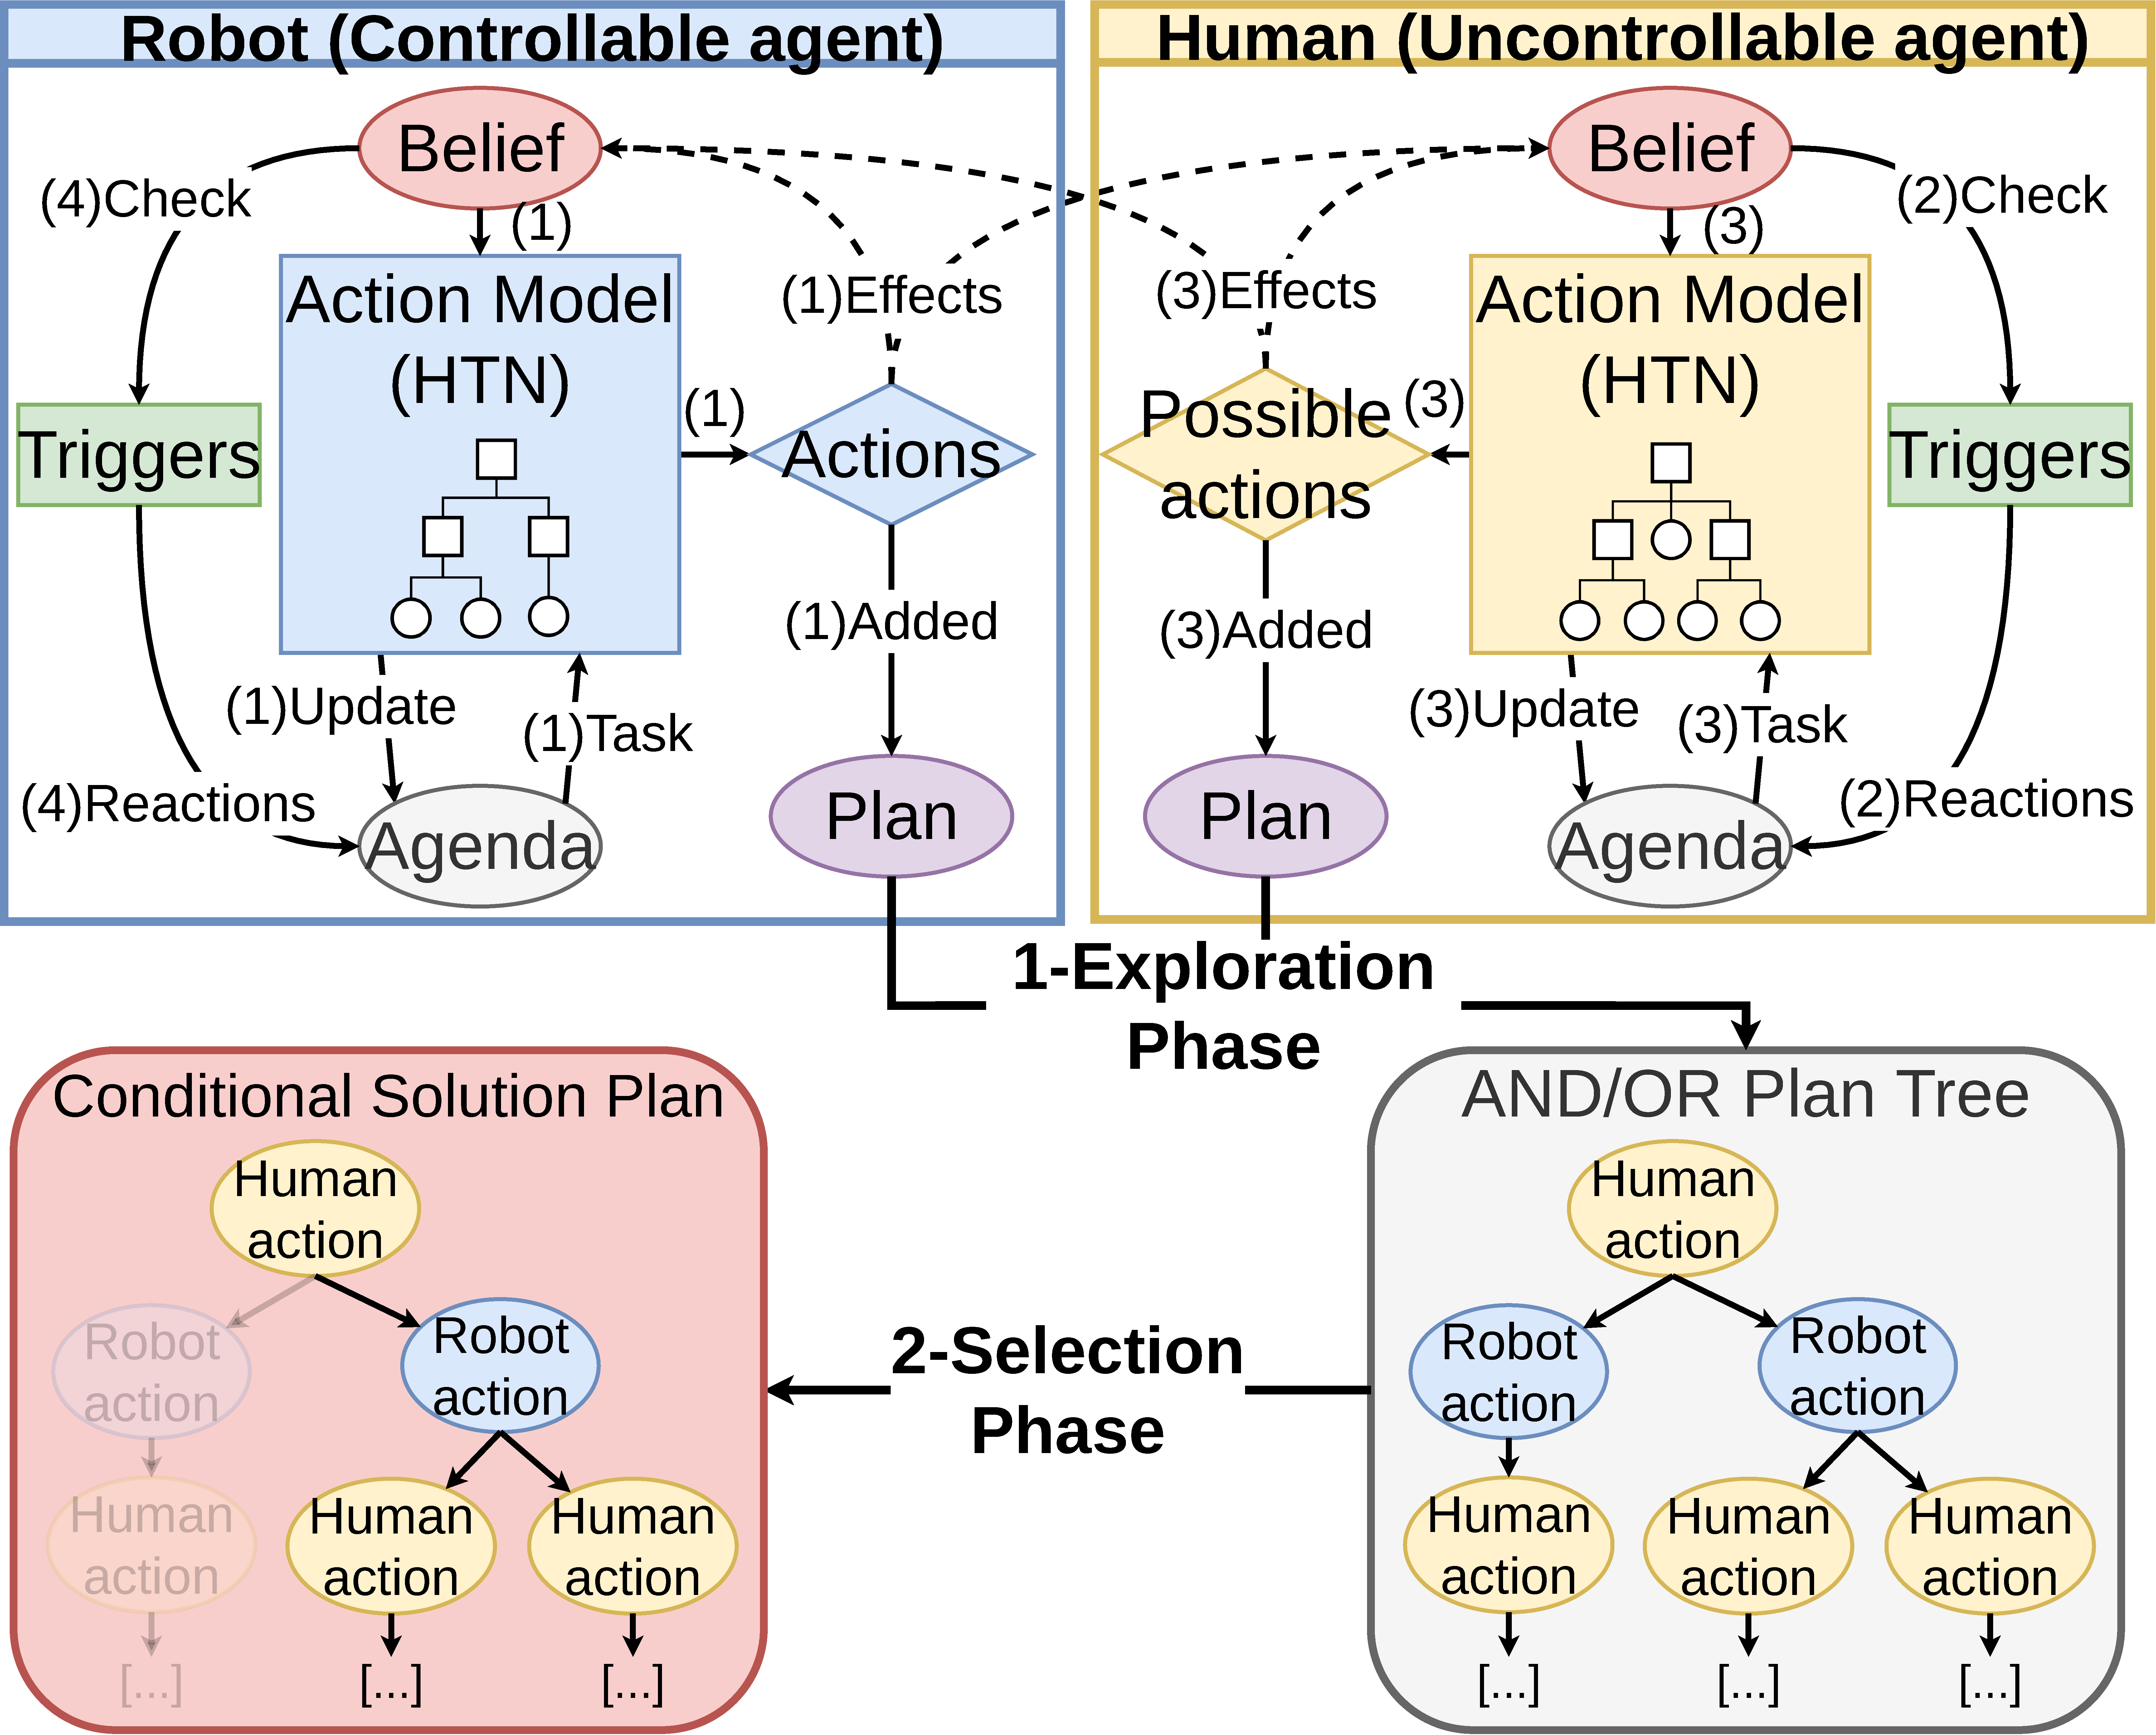
\includegraphics[width=\linewidth]{Chapter2/HATPEHDA_planning_process.pdf}
    \caption{The HTNs exploration consists in iterative loops of four steps : (1) Get possible robot actions from the robot HTN, add them to the plan and apply their specific effects on the H \& R beliefs, (2) Check Triggers and add the reactions in the corresponding agendas, (3) Get possible human actions based on their estimated beliefs, add them in the plan and apply their effects on the H \& R  beliefs, (4) Check Triggers again and add the reactions in the corresponding agendas. Here the robot is starting, but the human could with the following ordering: (3)>(4)>(1)>(2).}
    \label{fig:HATPEHDA_planning_process}
\end{figure}

The human \acrshort{htn} exploration differs from classical \acrshort{htn} planning as the goal is not to produce a complete plan but to list all the actions the human is likely to perform in a given agent state. 
We recursively decompose the first task of the human agenda $d^H$ with every applicable method until we reach an applicable operator. All the operators from all the applicable decompositions are returned to the robot HTN exploration and applied.

Two special cases are handled during the exploration. 
When an agent's agenda is empty, the exploration returns a default passive action \textit{IDLE}, which has no effect. It only indicates that the agent has nothing to do and will likely remain still. 
Besides, if no applicable action is found for an agent, the exploration returns a default passive action \textit{WAIT}. Similarly to \textit{IDLE}, it has no effect but represents the agent's impossibility to act in the current situation. 

Once both agendas are empty, the state is set as a success, the plan is added to the valid plans tree, and the search can continue until no decomposition is left for any task.


\section{Plan Evaluation and Selection}

In human-aware task planning, plan evaluation is a trade-off between efficiency and social criteria.
The robot should be efficient but also behave in an acceptable, legible, and accommodating manner.  


Cost evaluation is tricky because objective metrics are easy to use for efficiency. However, social criteria are more challenging to evaluate because they are hard to generalize. These social rules can be very context-dependent, making them hard to generalize and thus to take into account reliably.

Plan cost is a mix of all the following:

\begin{itemize}
    \item Length of the plan (number of actions or temporal duration if available).
    \item Sum of individual action cost: the cost of each action can be estimated to translate the effort required to perform it. It can reflect several aspects and constraints, such as pure physical strength required, duration of the action, or energy consumption.
    \item Undesired states: Common sense and social norms can be used to define several rules defining undesired states. This can cover various aspects such as hygiene or safety. For instance, despite being possible and maybe efficient, we would not like a robot holding a dirty dripping mop in one hand and the sandwich we asked for in the other hand. Another example is that we would not like a robot dropping a knife just on the edge of a table or counter because it may fall and be dangerous. 
    \item Undesired sequences of actions: For the same reasons, we can also define undesired sequences of actions. This can express preferences regarding the ordering of different subtasks, \textit{e.g.}, since we do not want the robot to hold our sandwich while cleaning the house, we would also not like the robot to clean first and then make a sandwich because the robot is likely to be dirty while making the sandwich.  
\end{itemize}

I implemented in HATP/EHDA a way to specify and take into account undesired state and action sequences. Detecting any of them in a possible plan would penalize the plan cost of the specified amount. Here, the undesired elements must be specified in the problem specification and are abstracted in the planner. However, as stated above, it is hard to generalize undesired states and action sequences and integrate them directly in the planner to avoid specifying them in the problem specification.

In HATP/EHDA, once the exhaustive exploration has been done, the result is a valid plan tree of alternating feasible robot and human actions along with their current beliefs leading to task completion. This second planning step aims to select robot actions, such as each human action in the plan has only one robot action as a child.
To do so, we define a cost function $cost: \sigma \times Op \mapsto \mathbb{R}^+$ representing the cost of an action in a specific state. The data structure is now similar to a two-player game tree. However, \textit{MinMax} approaches are unsuitable here, as we are not in an adversarial setup but more in a collaborative one. Indeed, trying to minimize the maximum possible cost assumes that humans will always do the actions that lead to the worst plan. This defensive behavior could lead to non-optimal plans. We thus propose to explore this tree differently.

Moreover, like in \acrshort{hatp}, we can define \textit{social costs} functions. These functions take a complete human and robot sequence of actions ($\pi^R$ and $\pi^H$) and return a cost ($\mathbb{R}^+$) which is added to the cost of the plan previously determined. By doing so, we can penalize non-acceptable sequence of robot actions (\textit{e.g.}serving a meal just after taking out the trash) or non-satisfactory human required contribution (\textit{e.g.}the robot requesting the human to perform small tasks multiple times instead of giving the big picture of the actual task to perform).

The approach we propose for plan selection is to minimize the average cost. It represents the human potentially selecting any course of action in their stream (while still respecting the action model defined in their HTN).
The algorithm is given the root action of the plan tree previously generated. It returns the cost of the conditional plan selected while selecting the robot actions in the plan tree to minimize the average plan cost.

\section{Qualitative Results}

Each scenario is commented on below with their corresponding selected plan shown in TABLE~\ref{tab:plans}.

The partial robot and human action models and their exploration are presented in Fig.~\ref{fig:plans}.

\begin{table}
\small
\begin{tabularx}{0.98\textwidth}{|X||X|}
    \hline
    \textbf{(a) \textit{R} and \textit{H1} build the stack together as a shared goal requested by \textit{H1}.}     & \textbf{(b) \textit{H1} requests to stack the cubes and \textit{R} acts alone.} \\
    \hline
    R-PickAndPlace(red, base)     & R-PickAndPlace(red, base) \\ 
    H1-PickAndPlace(red, base)     & R-moveTo(red) \\  
    R-PickAndPlace(green, bridge) & R-PickAndPlace(red, base) \\
    H1-PickAndPlace(blue, top)     & R-moveTo(init) \\
    R-PickAndPlace(yellow, top)   & R-PickAndPlace(green, bridge) \\
                                    & R-PickAndPlace(blue, top) \\
                                    & R-PickAndPlace(yellow, top) \\
    \hline \hline
    \textbf{(c) \textit{H1} requests R to build the stack, \textit{R} decides to punctually involve \textit{H2}.} & \textbf{(d) \textit{H1} requests R to build the stack, \textit{R} decides to invite H2 to a shared goal.} \\
    \hline
    R-PickAndPlace(red, base)     & R-PickAndPlace(red, base) \\
    H2-IDLE                        & H2-IDLE \\
    R-AskPunctualHelp(red)        & R-AskSharedGoal() \\
    H2-PickAndPlace(red, base)     & H2-PickAndPlace(red, base) \\
    R-PickAndPlace(green, bridge) & R-PickAndPlace(green, bridge) \\
    H2-IDLE                        & H2-PickAndPlace(blue, top) \\
    R-PickAndPlace(blue, top)     & R-PickAndPlace(yellow, top) \\
    H2-IDLE                        & \\
    R-PickAndPlace(yellow, top)   & \\
    \hline
\end{tabularx}
\caption{Execution trace of a selected plan for each scenario.}
\label{tab:plans}
\end{table}

\begin{sidewaysfigure}
    \centering 
    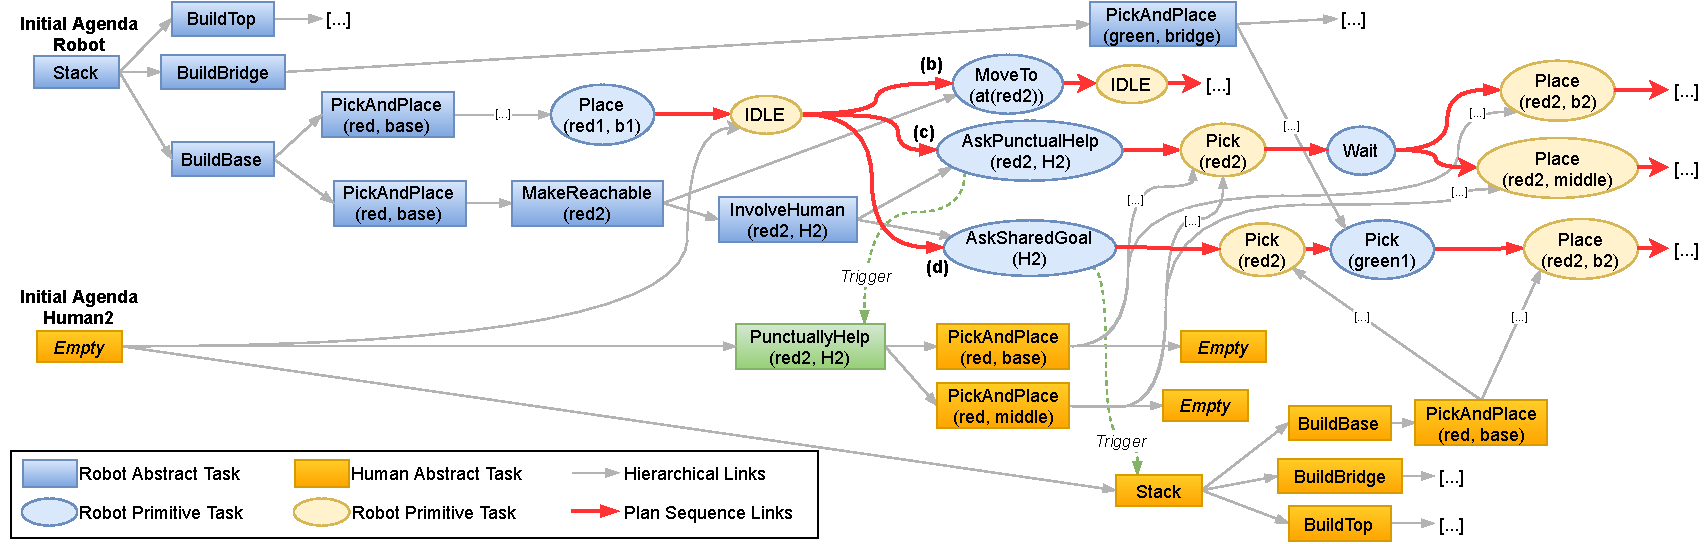
\includegraphics[width=1.0\textwidth]{Chapter2/plans.pdf}
    \caption{Illustration of the incremental exploration of various courses of actions corresponding to scenarios depicted in Fig.~\ref{fig:scenarios}(b), (c), and (d). Since \textit{H1} requests the robot to complete the task without establishing a shared goal, the robot agenda only contains the task to achieve, and the agenda of \textit{H2} starts empty.}
    \label{fig:plans}
\end{sidewaysfigure}

\paragraph{(a) \textit{H1} and R act together}
First, the human sets a shared goal by asking the robot to stack cubes with him. Since it is a shared goal, human and robot agendas are initialized with the ``Stack" task. Thus, the robot anticipates that the human will pick the unreachable second red cube by querying the human action model. Table~\ref {tab:plans}(a) shows the selected plan to collaboratively stack the cubes. 

\paragraph{(b) \textit{R} acts alone}
This time, the human asks the robot to stack the cubes but then leaves the scene, and the robot must act alone. Hence, the only applicable method to make the second red cube reachable is to move to the other side even though the movement action is expensive (we can imagine a table way longer than shown in the figure).

\paragraph{(c) \textit{R} asks punctual help}
The first human (\textit{H1}) requests the robot to complete the task, and another uninvolved human ($h2$) is present. The robot starts exploring its \acrshort{htn} and, thanks to the presence of the other human, a new method is applicable, allowing the robot to ask for help. It can ask for punctual help or a complete commitment of \textit{H2} to the task. Of course, asking for help for one cube is less costly than building the whole stack together. However, asking for help from someone not already involved in a common task is still expensive since they must put themselves in the task's context. 
Nevertheless, this punctual help is less costly for the robot than moving to the other side, so this solution is selected. Note that we model that after being asked to help punctually, the human can either stack the cube themself or make it reachable to the robot by placing it in the middle. Only the first branch is shown in table~\ref{tab:plans}(c), but the selected plan is in fact conditional with two branches as depicted in Fig.~\ref{fig:plans}.

\paragraph{(d) \textit{R} invites \textit{H2} to share a goal}
Same initial setup, but now two cubes are out of reach. Asking for punctual help is still less costly than moving around the table. 
However, each new request to \textit{H2} is assumed to be more and more costly, making repeated queries expensive.  
Therefore, due to the two unreachable cubes in this scenario, setting a shared goal becomes less costly for the robot than asking twice for punctual help.

\section{Conclusion}

What is offered by HATP/EHDA is very interesting. We rely and reason on the human model to plan the robot's actions while never compelling the human actions. The plan produced assumes turn-taking and no parallel execution of the actions. This is not a strict constraint as a post-analysis can reason on the causal links of the actions in the plan to extract a partially ordered plan to execute, making the execution more flexible. However, It is still a limitation addressed in Chapter~\ref{chap:4}.
\ifdefined\included
\else
\setcounter{chapter}{2} %% Numéro du chapitre précédent ;)
\dominitoc
\faketableofcontents
\fi

\chapter{Models and Algorithms for human-aware task planning with integrated theory of mind}
\chaptermark{Models and Algorithms of Theory of Mind}
\label{chap:3}
\minitoc


%%% SECTION %%%%%%%%%%%%%%%%%%%%%%%%%%%%%%%%%%%%%%%%%%%%%%%%%%%%
\section{Introduction}

We would want the robot to be able to reason and maintain correctly the distinct human beliefs. Despite modeling distinct beliefs, HATP/EHDA doesn't maintain in a principled way, only in a scripted way (domain specific). Here we propose some models and algorithms to integrate some concept of Theory of Mind in the planning process of HATP/EHDA. This way, the robot can estimate more accurately the human's belief to predict their behavior. Moreover, we propose solutions for the robot when to tackle estimated false human beliefs that may impact the task resolution.

Explaining false belief task (Sally and Anne)
\begin{figure}
    \centering
    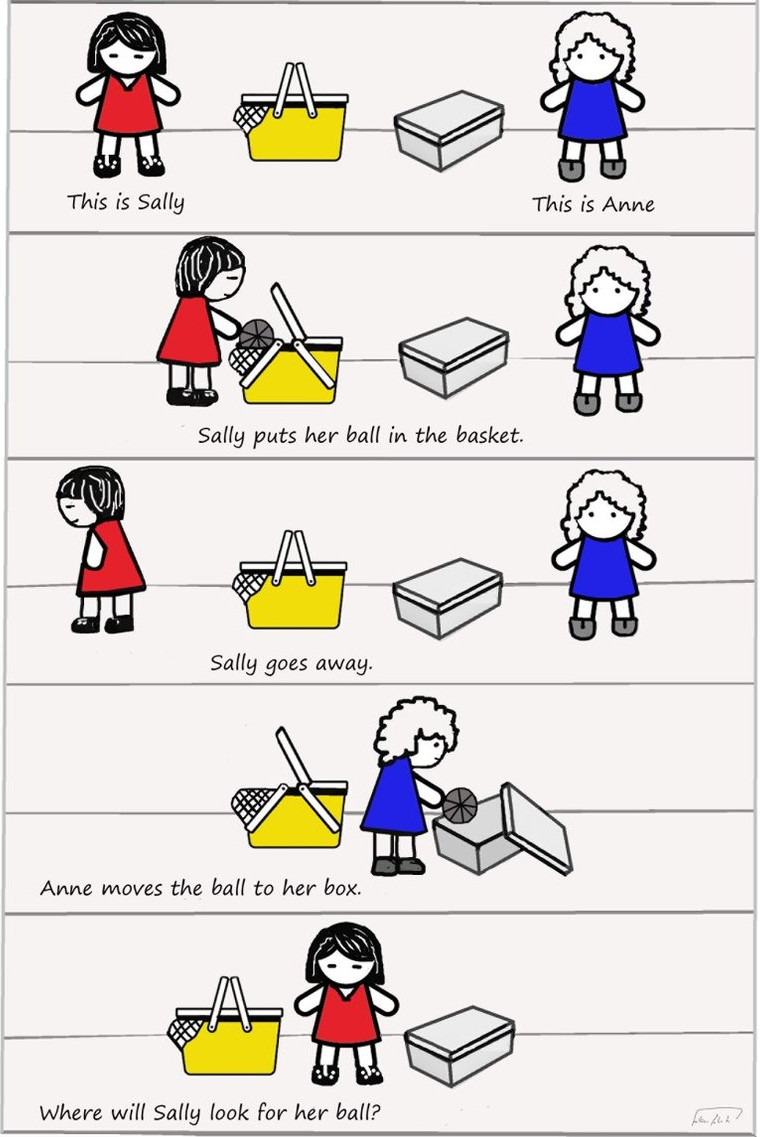
\includegraphics[width=0.5\linewidth]{images/Chapter3/The-Sally-Anne-Task.jpeg}
    \caption{Sally and Anne Task}
    \label{fig:sally_and_anne_ask}
\end{figure}



%%% SECTION %%%%%%%%%%%%%%%%%%%%%%%%%%%%%%%%%%%%%%%%%%%%%%%%%%%%
\section{Related works}

    This chapter's contribution is related to several topics not mentioned yet. Hence, to better capture the contribution, this section introduces the new topics and relevant related works.  

    %%% SUB-SECTION %%%%%%%%%%%%%%%%%%%%%%%%%%%%%%%%%%%%%%%%%%%%
    \subsection{Epistemic planning}
    Epistemic planning plays a crucial role in human-robot collaboration. It allows robots to reason about their own knowledge and beliefs, as well as the knowledge and beliefs of other agents \cite{bramblett_epistemic_2023}. This is important for coordination and collaboration among multiple agents, as success can only be expected if agents can reason about each other's knowledge, uncertainty, and capabilities \cite{bramblett_epistemic_prediction_2023}. Epistemic planning is used in various application areas, including mobile service robots, explaining planning, game playing, human-robot interaction, and social robotics \cite{hu_planning_2023}. It enables robots to make plans to achieve the required knowledge and to reason about the knowledge and capabilities of other agents, ensuring effective collaboration and coordination in human-robot interactions \cite{belle_epistemic_2023}.


    Def. Thomas Bolander is one of the main contributor to this field. Proposed the DEL approach. \cite{bolander_gentle_2017} and extended it.

    ``Automated planning is a branch of artificial intelligence concerned with computing plans (sequences of actions) leading to some desired goal. A human or robot could e.g. have the goal of picking up a parcel at the post office, and then the problem becomes to find a successful sequence of actions achieving this. Epistemic planning is the enrichment of planning with epistemic notions, that is, knowledge and beliefs. The human or robot might have to reason about epistemic aspects such as: Do I know at which post office the parcel is? If not, who would be relevant to ask? Maybe the parcel is a birthday present for my daughter, and I want to ensure that she doesn't get to know, and have to plan my actions accordingly (make sure she doesn't see me with the parcel). The epistemic notions are usually formalized using an epistemic logic. Epistemic planning can naturally be seen as the combination of automated planning with epistemic logic, relying on ideas, concepts and solutions from both areas.''

    Muise et al. worked on multi-agent epistemic planning using a classical planning approach. Since involving nested beliefs is computationally demanding, their work proposes to convert and encode such problems into classical planning problems. Hence, state-of-the-art classical planning technics can be used to tackle nested beliefs of multiple agents problems. 

    \subsection{Theory of Mind in HRC}
    Epistemic planning helps to plan the correct sequence of actions to perform to reach a desired knowledge, including a desired world state. However, estimating the current knowledge and beliefs of the different agents is challenging. To do so, we have to consider Theory of Mind concepts, especially perspective shift and the notion of co-presence. Some epistemic planning works already integrate of ToM notions, but the subject is worth being discussed a bit more in details. Indeed, in the HRI field, ToM is used in various domains like navigation, dialogue and like here in task planning. 

    Theory of mind (ToM) plays a crucial role in task planning for human-robot collaboration. 
    ToM refers to the ability to attribute mental states to oneself and others, such as beliefs, desires, and intentions. 
    
    (v1) Robots endowed with ToM abilities can anticipate and understand the mental states of their human partners, allowing for more effective interaction and decision-making. By inferring their partner's trust and strategy, robots can adjust their own decision models and policies to optimize team performance [1]. Mimicking ToM in robots influences human decision-making behavior and trust, making it more appropriate and conducive to collaboration [2]. Robots implementing ToM are perceived as more socially intelligent and helpful, enhancing the quality of human-robot interactions [3]. Computational theory of mind, based on abstractions of beliefs into higher-level concepts, enables agents to reason and collaborate with humans efficiently, improving decision-making outcomes [4]. However, the field lacks a unified construct and consistent benchmarking, hindering progress in endowing robots with ToM capabilities [5].

    (v2) Robots endowed with ToM abilities are more effective in proactive robotic assistance and are perceived as more socially intelligent by humans \cite{shvo_proactive_2022}. ToM enables robots to infer human desires, beliefs, and intentions, allowing for natural interaction between robots and humans \cite{yu_robot_2023}. Robots with ToM can anticipate human strategies and incorporate them into their decision models, leading to better team performance \cite{romeo_exploring_2022}. The presence of ToM in robots influences human decision-making behavior and trust, making it more appropriate for human-robot collaboration \cite{schlobach_abstracting_2022}. Computational theory of mind, based on abstractions of beliefs into higher-level concepts, facilitates collaboration on decisions and improves the quality of human decisions \cite{gurney_robots_2022}. However, the lack of a unified construct and consistent benchmarking hinders progress in endowing robots with ToM capabilities.

    \textbf{TODO: Merge two versions, but references of v1 are not accessible anymore...}

    
    \subsection{Communication in HRC}

    Communication plays a crucial role in human-robot collaboration. It enables effective interaction between humans and robots, promoting inclusivity and reducing obstacles in human-robot interaction. Communication allows robots to share information about their actions and intentions, enhancing transparency and explainability \cite{mcmillan_human-robot_2023}. It helps in establishing trust and understanding between humans and robots, leading to improved teamwork and performance \cite{verhagen_influence_2022}. Non-verbal gestures and behavior of robots during collaboration can impact the perception of the robot and influence the willingness of humans to cooperate \cite{arntz_collaborating_2022}. Communication also allows robots to assess their own skills and limitations, propose alternatives, and adapt the execution of tasks to the capabilities of the collaborators \cite{ferrari_bidirectional_2022}. Overall, effective communication facilitates mutual knowledge, enables the exchange of information, and allows humans and robots to work together efficiently and successfully.


%%% SECTION %%%%%%%%%%%%%%%%%%%%%%%%%%%%%%%%%%%%%%%%%%%%%%%%%%%%
\section{Maintaining the human beliefs}

    %%% SUB-SECTION %%%%%%%%%%%%%%%%%%%%%%%%%%%%%%%%%%%%%%%%%%%%
    \subsection{Enhanced problem specification}

\textbf{TODO: switch from 'we' to 'I'?}

\begin{figure}[t!]
    \centering
    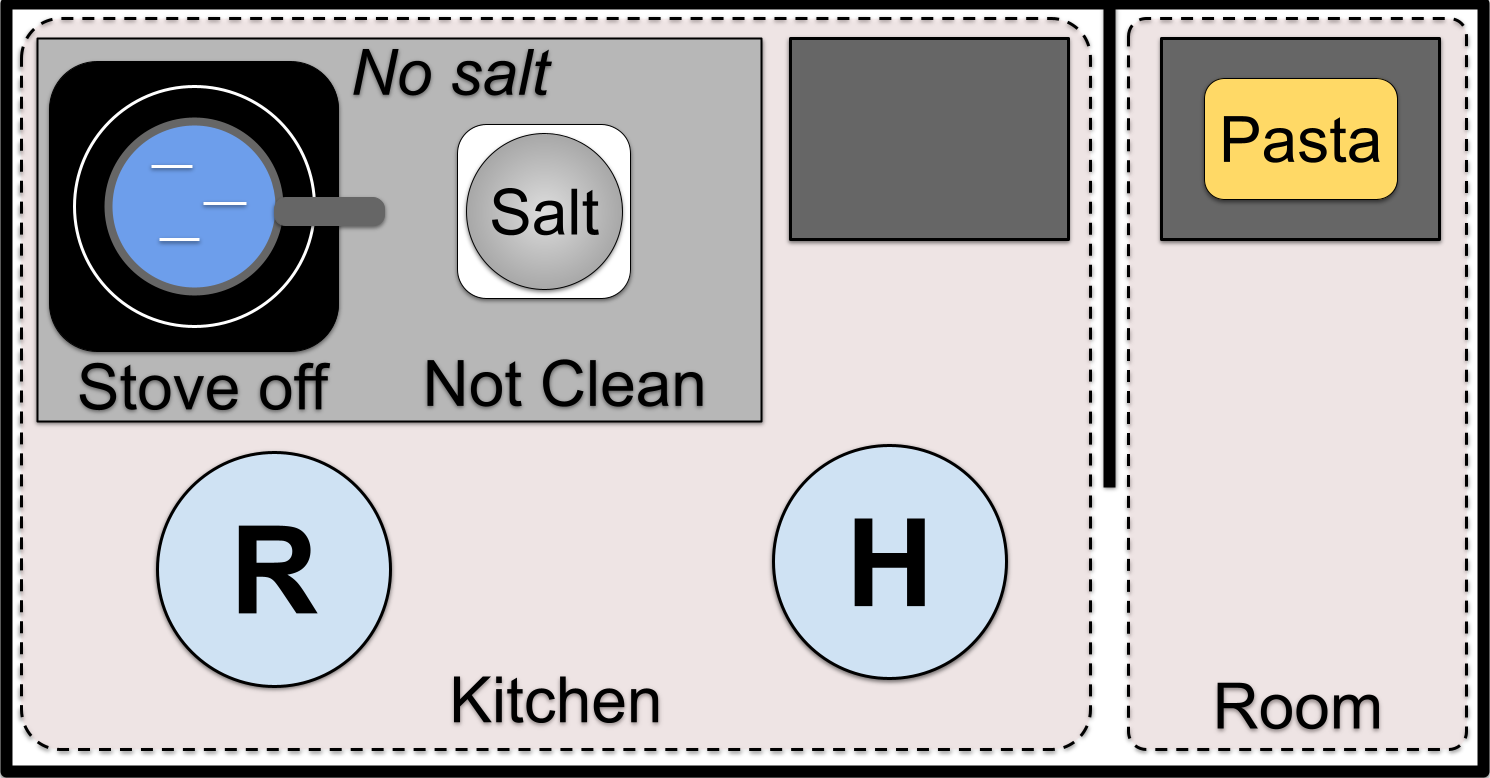
\includegraphics[width=0.70\linewidth]{images/Chapter3/cooking_task_draw.png}
    \caption{
    Let us consider cooking pasta as a human-robot shared task. 
    The robot has to turn on the stove (\textit{stoveOn}) and clean the counter (\textit{counterClean}), but the latter is not a part of the shared task. The human takes care of fetching the pasta while both agents can add salt into the water (\textit{saltIn}). Before pouring the pasta into the pot the human must know the facts, \textit{stoveOn} and \textit{saltIn}. 
    Unlike \textit{stoveOn}, the facts \textit{saltIn} and \textit{counterClean} are not directly observable. 
    Hence, by acting while the human is away to fetch the pasta, the robot may induce false beliefs which may be detrimental to the shared task (e.g., human adding salt again).
    }
    \label{fig:new_scene}
\end{figure}

We start from the HATP/EHDA probleme specification which is the following.

We consider a \textit{classical planning domain} (\textit{state-transition system}) $\Sigma = (S,A,\gamma)$, s.t., $S$ is a finite set of states in which the system may be, $A$ is a finite set of actions that the actors may perform, $\gamma : S \times A \rightarrow S$ is a state-transition function. Each state $s \in S$ is a description of the properties of various objects in the planner's environment~\cite{naubooks0014222}. 

To represent the objects and their properties, we will use two sets $B$ and $X$: $B$ is a set of names for all the objects, plus any mathematical constants representing properties of those objects. $X$ is a set of syntactic terms called state variables, s.t. the value of each $x \in X$ depends solely on the state $s$.

A \textit{state-variable} over $B$ is a syntactic term $x = sv(b_1, ..., b_k)$, where $sv$ is a symbol called the state variable's name, and each $b_i$ is a member of $B$ and a parameter of $x$. Each state variable $x$ has a range, $\textit{Range}(x) \subseteq B$, which is the set of all possible values for $x$.

Here is the description of the sets $B$ and $X$ for the collaborative cooking example:
{\small
\begin{align*}
&B           = Entities \cup Places \cup Booleans \cup \{\textsf{nil}\} \\
&\quad Entities    = Agents \cup Objects\\
&\quad Agents      = \{ \textsf{R}, \textsf{H} \} ~~ \backslash\backslash~\textsf{R}:robot,~\textsf{H}:human\\
&\quad Objects     = \{ \textsf{salt}, \textsf{pasta}, \textsf{counter} \}\\
&\quad Places      = \{ \textsf{kitchen}, \textsf{room} \}\\
&\quad Booleans    = \{ \textsf{true},\textsf{false} \}\\
&\\
&X = \{ at(e), saltIn, stoveOn, counterClean ~ | ~ e \in Entities \}\\
&\quad \textit{Range}(saltIn ~|~ stoveOn ~|~ counterClean)=Booleans\\
&\quad \textit{Range}(at(\textsf{R} ~|~ \textsf{H} ~|~ \textsf{pasta})) = Places\\
&\quad \textit{Range}(at(\textsf{salt} ~|~ \textsf{counter})) = \{ \textsf{kitchen} \}
\end{align*}
}

A \textit{variable value assignment} function over $X$ is a function $val$ that maps each $x_i \in X$ into a value $z_i \in$ $\textit{Range}(x_i)$. With $X = \{ x_1, ..., x_n \}$, we will often write this function as a set of assertions: $val = \{ x_1=z_1, \ldots, x_n=z_n \}$. 

Our first contribution starts from here where we augmented the specification by associating each state variable to a location and to an observability type.

A \textit{variable observability assignment} function over $X$ is a function $obs$ that maps each $x_i \in X$ into an observability type $t_i \in \{ \texttt{OBS},  \texttt{INF} \}$: $obs = \{ (x_1,t_1), \ldots , (x_n,t_n) \}$. Respectively, when $obs(x_i) = \texttt{OBS} | \texttt{INF}$ then $x_i$ is said to be \textit{observable} $|$ \textit{inferable} in the state $s_i$.

A \textit{variable location assignment} function over $X$ is a function $loc$ that maps each $x_i \in X$ into a $l_i \in Places \cup \{ \texttt{nil} \}$: $loc = \{ (x_1,l_1), ..., (x_n,l_n) \}$. 
$Places \subseteq B$ captures a group of constant symbols such that each member is a predefined area in the environment. 
Agents are always either ``situated'' in a place or moving between two places. 
We consider $x_i$ to be located in every $place \in Places$ if $loc(x_i)=\texttt{nil}$. 
More details about how the environment should be divided into places will be given shortly.

A \textit{state} $s_i \in S$ is a 6-tuple composed of 4 functions over $X$ and 2 task networks (agendas)  s.t. $s_i = (val_i, val^H_i, obs_i, loc_i, tn^R_i, tn^H_i)$. 
The state of the world from the perspective of the robot is captured by the variable value assignment function $val_i$, sometimes noted as $val^R_i$. 
Similarly, $val^H_i$ represents the estimation of $val_i$ in the perspective of the human, also referred to as the estimated human beliefs. 
Hence, $\forall s_i \in S$, each $x_j \in X$ is  mapped to two \textit{values} (robot perspective and estimation of human's beliefs), an \textit{observability type}, and a \textit{place}. We say that a state $s_i \in S$ contains \textit{false beliefs}, or \textit{belief divergences}, if $\exists x_j \in X, val^H_i(x_j) \neq val^R_i(x_j)$. 

For our example, the initial state $s_0$ would be as follow: 

\newcommand{\smallvspace}{\vspace{-0.8cm}}
\newcommand{\bigvspace}{\vspace{-1.3cm}}

{\small
\noindent
\begin{multline*}
s_0 = \{val_0, ~val^H_0, ~obs_0, ~loc_0, ~tn^R_0, ~tn^H_0\} \\ \quad
\end{multline*}
\bigvspace
\begin{multline*}
\quad val_0 = val^H_0 = \{at(\textsf{R}) = \textsf{kitchen}, at(\textsf{H}) = \textsf{kitchen},\\ 
at(\textsf{pasta}) = \textsf{room}, saltIn = \textsf{false}, stoveOn=\textsf{false} \}
\end{multline*}
\smallvspace
\begin{multline*}
\quad obs_0=\{ (at(e),\texttt{OBS}),
(saltIn,\texttt{INF}),
(stoveOn,\texttt{OBS})\\
(counterClean,\texttt{INF}),
~|~ e \in Entities \}
\end{multline*}
\smallvspace
\begin{multline*}
\quad loc_0=\{ (at(e),val_0(e)),
(counterClean,\textsf{kitchen}),\\
(saltIn,\textsf{kitchen}),
(stoveOn,\textsf{kitchen}),
~|~ e \in Entities \}
\end{multline*}
\smallvspace
\begin{multline*}
\quad tn^R_0 = \{ CookPasta, CleanCounter \} \\ \quad
\end{multline*}
\bigvspace
\begin{multline*}
\quad tn^H_0 = \{ CookPasta \} \\ \quad
\end{multline*}
\smallvspace
}

An action is a tuple $\alpha = (\textit{head}(\alpha), \textit{pre}(\alpha), \textit{eff}(\alpha))$ where $\textit{head}(\alpha)$ is a syntactic expression of the form $\textit{act}(z_1, ..., z_k)$ where $act$ is a symbol called the \textit{action name} and $z_1,...,z_k$ are variables called parameters. $\textit{pre}(\alpha) = \{ p_1, ..., p_m \}$ is a set of preconditions, each of which is a literal. And $\textit{eff}(\alpha) = \{ e_1, ..., e_n \}$ is a set of effects, each of which is an expression of the form: $sv(t_1, ..., t_j) \leftarrow t_0$ with $t_0$ being either the value to assign to the state variable $sv(t_1, ..., t_j)$ or a new location/place for the state variable. We note $\textit{agt}(\alpha)$ the agent performing the action $\alpha$.

To estimate the next possible actions that an agent $\varphi \in Agents$ is likely to perform in a state $s_i \in S$, we proceed in the same way as in~\cite{buisan:hal-03684211}. We refine the agent's agenda $tn_{\varphi}$ based on its belief $val^\varphi_i$ and obtain a \textit{refinement} as follows $\textit{ref}(tn^\varphi_i, val^\varphi_i)= \{ (a_1,tn_1),...,(a_j,tn_j) \}$. 
A \textit{refinement} contains a tuple for each estimated possible action $a_j$ and the associated new agenda $tn_j$ after being refined. 

In our cooking example, we obtain the following refinement if the starting agent is the human:\\
{\small
$\textit{ref}(tn^H_0, val^H_0) = \{ (add\_salt(),tn_1), (move\_to(\textsf{kitchen}),tn_2) \}$
}


    %%% SUB-SECTION %%%%%%%%%%%%%%%%%%%%%%%%%%%%%%%%%%%%%%%%%%%%
    \subsection{State Transitions and Beliefs Updates}
Learn from observation of either: action execution or observable state.

Assumption 1 : We do not consider uncertainties. Thus, agents are either wrong or right about the state of the world but never uncertain. This would be an interesting future work. 

Assumption 2 : We do not consider cases where the robot's beliefs can diverge. Since the planner is part of the robot, the actual ground truth is unknown. We can only assume that the estimation of the state of the world by the robot is correct and reason on it.

Assumption 3 : Coming from the two previous assumptions, we assume that the human only makes deterministic moves when not being observed. Hence, regardless of being co-present, the robot's beliefs are always updated with the action's effects.


Thus, $\forall x \in X$, we always have,

\begin{equation}
    val_{i+1}(x) = \left\{ 
    \begin{array}{ll}
        w, & \mbox{if} ~ x \leftarrow w \in \textit{eff}(a)   \\ 
        val_i(x), & \mbox{otherwise}
    \end{array}\right.
\end{equation}

The place associated with a state variable can be modified by the action's effect but, here, we assume that the observability type of each fact is constant during the task. So, $\forall x \in X$,

\begin{align}
    &obs_{i+1}(x) = obs_i(x)\\
    &loc_{i+1}(x) = \left\{ 
    \begin{array}{ll}
        l, & \mbox{if} ~ x \leftarrow l \in \textit{eff}(a)\\
        loc_i(x), & \mbox{otherwise}
    \end{array}\right.
\end{align}

The new agenda of each agent ($tn^R_{i+1}, tn^H_{i+1}$) are created by the HTN refinement algorithm, and thus, they are directly retrieved from the obtained refinement. 
This refinement decomposes abstract tasks in the task network until the first task is a primitive action. To do so, every applicable method is applied leading to a set of possible actions (and refined task networks).

The new estimated human belief $val^H_{i+1}$ is the two-step result of our Situation Assessment processes that models the human's real-time sensing and reasoning capabilities about their surroundings.

First, let us define the notions of \textit{co-presence} and \textit{co-location} which will be key to maintaining the evolution of agents' beliefs as planning progresses.

\begin{definition} \label{def:co-pre-loc}
    \textbf{(Co-presence \& Co-location.)} In a state $s_i \in S$, two agents, $\varphi_1$ and $\varphi_2$, are considered to be \textit{co-present} if $val_i(at(\varphi_1)) = val_i(at(\varphi_2))$. This relation is noted $\varphi_1 \curlywedge_i \varphi_2$ in the rest of the paper. Similarly, we say that an agent $\varphi_1$ is \textit{co-located} with a state variable $x \in X$ if $val_i(at(\varphi_1)) = loc_i(x)$, noted $\varphi_1 \curlywedge_i x$.
\end{definition}

Now we can define two SA processes that will maintain the estimated human beliefs.

\begin{definition} \label{def:new_inf}
    \textbf{(Inference Process.)} An agent observes the execution of an action by being either co-present with the acting agent, 
    or by being the acting agent. If so, the agent infers the new values of every state variable present in the action's effects.
\end{definition}

Based on the above definition, the human's beliefs are updated as follows when action $a$ is executed in state $s_i$, 

\begin{equation}
val'^H_{i+1}(x) = \left\{ 
\begin{array}{ll}
    w, & \mbox{if} ~ x \leftarrow w \in \textit{eff}(a) ~ \mbox{and}  \\ 
    & (H = \textit{agt}(a) ~\mbox{or}~ H \curlywedge_i \textit{agt}(a)\\
    & ~\mbox{or}~ H \curlywedge_{i+1} \textit{agt}(a))\\
    val^H_i(x), & \mbox{otherwise}
\end{array}\right.
\end{equation}

To change its \textit{place} in the environment, agents would use a dedicated \textit{``move''} action, such that its effect only updates the agent's location. 

\begin{definition} 
\label{def:new_obs}
    \textbf{(Observation Process.)} An agent observes its surroundings and assesses the exact value of each state variable located in the same place (i.e., each state variable the agent is co-located with).
\end{definition}

After applying the effects of an action to obtain $val_{i+1}$ and the human beliefs $val'^H_{i+1}$ (using the inference process), the observation process is executed. It updates again the estimated human beliefs with the facts currently observable by the human and provides fully updated human beliefs to store in the state $s_{i+1}$, $\forall x \in X$:

\begin{equation}
val^H_{i+1}(x) = \left\{ 
\begin{array}{ll}
val_{i+1}(x), & \mbox{if}~ H \curlywedge_{i+1} x ~\mbox{and}~ \\
    & obs_{i+1}(x) = \texttt{OBS}\\
val'^H_{i+1}(x), & \mbox{otherwise}
\end{array}\right.
\end{equation}

Note that before starting the planning process, the observation process is executed once on the initial state $s_0$. This allows us to potentially correct the estimated human beliefs with the facts the human should initially be able to observe. 

The definition of the set $Places$, i.e. how the environment is divided into different \textit{places}, is guided by the shape of our state transition function. Hence, a $place \in Places$ is an area in the environment such that, when situated in it, agents are aware of each other's activity and they can assess every observable fact located in it. 

Note that unlike in DEL~\cite{KR2021-12}, our knowledge representation is simple and prevents us from expressing agents being \textit{uncertain} about a fact. 
In line with the classical closed-world assumptions, agents either know the truth or have a false belief w.r.t. the ground truth. 
We consider a straightforward scenario in which the human is \textit{``unaware''} of non-observed changes in the environment. 
This results in estimated false human beliefs, helping to detect whether a non-observed robot action can disrupt a seamless collaboration. 

%%% SECTION %%%%%%%%%%%%%%%%%%%%%%%%%%%%%%%%%%%%%%%%%%%%%%%%%%%%
\section{Relevant False human beliefs}

In this section, we explain our procedure to detect \textit{when} a false human belief should be corrected and \textit{how}.


    %%% SUB-SECTION %%%%%%%%%%%%%%%%%%%%%%%%%%%%%%%%%%%%%%%%%%%%
    \subsection{Detection}

The human and the robot carry individual distinct beliefs, while the two can be aligned, or diverging when the human has a false belief. To produce a legal solution plan the robot is fine with such false human beliefs unless they are qualified as \textit{relevant} (Definition~\ref{def:relevant_false_belief}). In such cases, the relevant false belief needs to be tackled.

\begin{definition} \label{def:relevant_false_belief}

A \textbf{relevant false belief} is a false belief that influences the next action(s) the human is likely to perform, either in terms of number, name, parameters, or effects. This can be written as follows:
A state $s_i$ contains a relevant false belief if either (\ref{eq:rel_div_cond_1}) or (\ref{eq:rel_div_cond_2}) is true:

\begin{equation} \label{eq:rel_div_cond_1}
ref(tn^H_i, val^H_i) \neq ref(tn^H_i, val^R_i)
\end{equation}
\begin{equation} \label{eq:rel_div_cond_2}
\{ \gamma(s_i,a) ~|~ \forall a \in ref( tn^H_i, val^H_i ) \} \neq \{ \gamma(s_i,a) ~|~ \forall a \in ref( tn^H_i, val^R_i ) \}
\end{equation}
\end{definition}

We consider that as soon as a false belief has an effect on human actions it should be tackled. An interesting future work could  be to check in a principled way the overall positive and detrimental impacts of this false belief on collaboration. But it is out of the scope of this work.

    %%% SUB-SECTION %%%%%%%%%%%%%%%%%%%%%%%%%%%%%%%%%%%%%%%%%%%%
    \subsection{Resolution with minimal communication}

A state containing a false human belief marked as \textit{relevant} must be handled. 
The first way to do it is by planning communication actions such that the robot communicates only the required facts to the human. This allows to correct false human beliefs that are relevant, but false beliefs that are \textit{``non-relevant''} will remain. 

\subsubsection{Modeling Communication Actions} 
We propose a generic communication action schema ($ca$) in this context. 
An agent $\varphi_i$ can \textit{communicate} an assertion $x=z$ (with $x \in X$ and $z \in$ Range($x$)) \textit{via} the action $ca_{\varphi_i, \varphi_j}(x,z)$ if $val^{\varphi_i}(x) = z$ and $val^{\varphi_j}(x) \neq z$.
The effect of $ca_{\varphi_i, \varphi_j}(x,z)$ corresponds to $val^{\varphi_j}(x) \leftarrow z$. Such actions are considered equally costly and instantaneous.

\subsubsection{Communicate Only the Required Facts}
Definition~\ref{def:relevant_false_belief} indicates if there is at least one diverging state variable in the human beliefs causing adverse effects, but without identifying which one(s).
Hence, we explain a subroutine below with the three steps, describing how we first identify the pertinent state variables to align, and then how the corresponding communication actions are created and inserted into the robot's plan.

\begin{enumerate}
    \item 
    \textit{Store} each state variable whose value differs in the human beliefs from the robot beliefs: $X_{diff} = \{ x ~|~ x\in X, val^H_i(x) \neq val^R_i(x) \}$.

    \item
    \textit{Build}, for each stored state variable $x \in X_{diff}$, a communication action $ca_{R, H}(x,val^R_i(x))$, all stored in a set $\mathit{CA}_{diff}$.

    \item 
    \textit{(Breadth-First Search.)} 
    The \textit{source} is $s_i$. Applying each $ca \in \mathit{CA}_{diff}$ generates a new state by aligning \textit{exactly} one state variable in the human beliefs s.t. $s'_i = \gamma(s_i, ca )$. 
    The search continues until the first state $s'_i$ selected to expand doesn't contain a relevant false belief. The communication actions used from the root until this selected state are \textit{retrieved} in a set $\mathit{CA}$.
\end{enumerate}

Once the above subroutine finishes, the retrieved communication actions in the set $\mathit{CA} = \{ ca_{R, H}(x_1,val^R_i(x_1)),..., ca_{R, H}(x_j,val^R_i(x_j)) \}$ must be inserted in the plan for belief alignment. Thus, Definition~\ref{def:joint-sol-plan} is redefined to be sound w.r.t. our approach. An edge can now either be a human action $o^h$ or a robot action $o^r$ with a set of communication action $CA$.
At each step, humans perform \textit{Observation}, while the robot executes each communication action $ca \in \mathit{CA}$, making the human's belief to \textit{update instantaneously}.

The set $\mathit{CA}$ is inserted before the diverging human actions and after the closest state where agents are co-present. 
But it could be interesting to reason with a better plan evaluation system to find the best place to insert this set.

    %%% SUB-SECTION %%%%%%%%%%%%%%%%%%%%%%%%%%%%%%%%%%%%%%%%%%%%
    \subsection{Resolution by delaying non-observed robot action}

So far we relied on communication, but depending on the environment (e.g. noisy), communication can be cognitively demanding. 
Thus, when the relevant false belief is due to a non-observed robot action, we propose to also consider implicit communication by postponing the pertinent robot action until the human is estimated to be observing its execution. 
This prevents false beliefs from even occurring.

First, a branch using communication is explored and the state variables concerned by the relevant false beliefs are retrieved (through all $ca \in CA$).
Then we check if the divergence is produced by a non-observed action. For now, it is done by checking if the relevant divergence concerns only one inferable state variable and if it was not present in the initial state.   
After, we identify which action creates the divergence by sequential regressing the current branch/trace. Hence, we can identify when the relevant divergence appears and which action should be delayed.
Once identified, we create another branch in the plan just before the identified action. In this new branch, {\sc delay} actions are inserted in the robot's plan until the human is co-present. When the human is co-present again, the identified action is inserted and observed by the human. Then the nominal planning process is resumed.  

%%% SECTION %%%%%%%%%%%%%%%%%%%%%%%%%%%%%%%%%%%%%%%%%%%%%%%%%%%%
\section{Result}

Referring to the related work section, we are not aware of an implemented planning system that can be used as a baseline. Hence, we use the HATP/EHDA solver to help present our approach's results on three \textit{novel} planning domains.

\subsubsection{Cooking Pasta Domain}
The running example corresponds to a specific problem in this domain. In fact, agents and pasta can initially either be in the kitchen or in the adjacent room, the stove might be on or off and there might be salt or not in the water.  
In the results, we will focus on the following three state variables from $X$. Both $stoveOn$ ($\texttt{OBS}$) and $saltIn$ ($\texttt{INF}$) are relevant to the human, unlike $Clean$ ($\texttt{INF}$) which only concerns the robot. 

\subsubsection{Preparing Box Domain}
A box with a sticker on it and filled with a fixed number of balls is considered prepared and needs to be sent. Both agents can \textit{fill} the box with balls from a bucket, while only the robot can \textit{paste} a sticker and only the human can \textit{send} the box. The bucket can run out of balls, so when one ball is left, the human \textit{moves} to another room to \textit{grab} more balls and \textit{refill} it. 
The number of balls in the box is \textit{inferable}, while all other variables are {\em observable}. 
In the following, three boxes have been considered.

\subsubsection{Car Maintenance Domain}
The washer fluid ($\texttt{OBS}$) and engine oil ($\texttt{INF}$) levels have to be \textit{full} before \textit{storing} the oil gallon in the cabinet ($\texttt{INF}$). 
Only the robot can \textit{refill} both the tanks and store the gallon while situated at \textit{Front} of the car. 
\textit{Front-left} and \textit{Front-right} headlights have to be \textit{checked} and a light-bulb has to be \textit{replaced} at \textit{Rear}. 
Only the human can check and replace lights, and they can start with either of these two tasks.
Both agents start at \textit{Front}.
The car's hood needs to be \textit{closed} by the human at last.

\subsection{Qualitative Analysis}

\begin{figure}[t!]
    \centering
    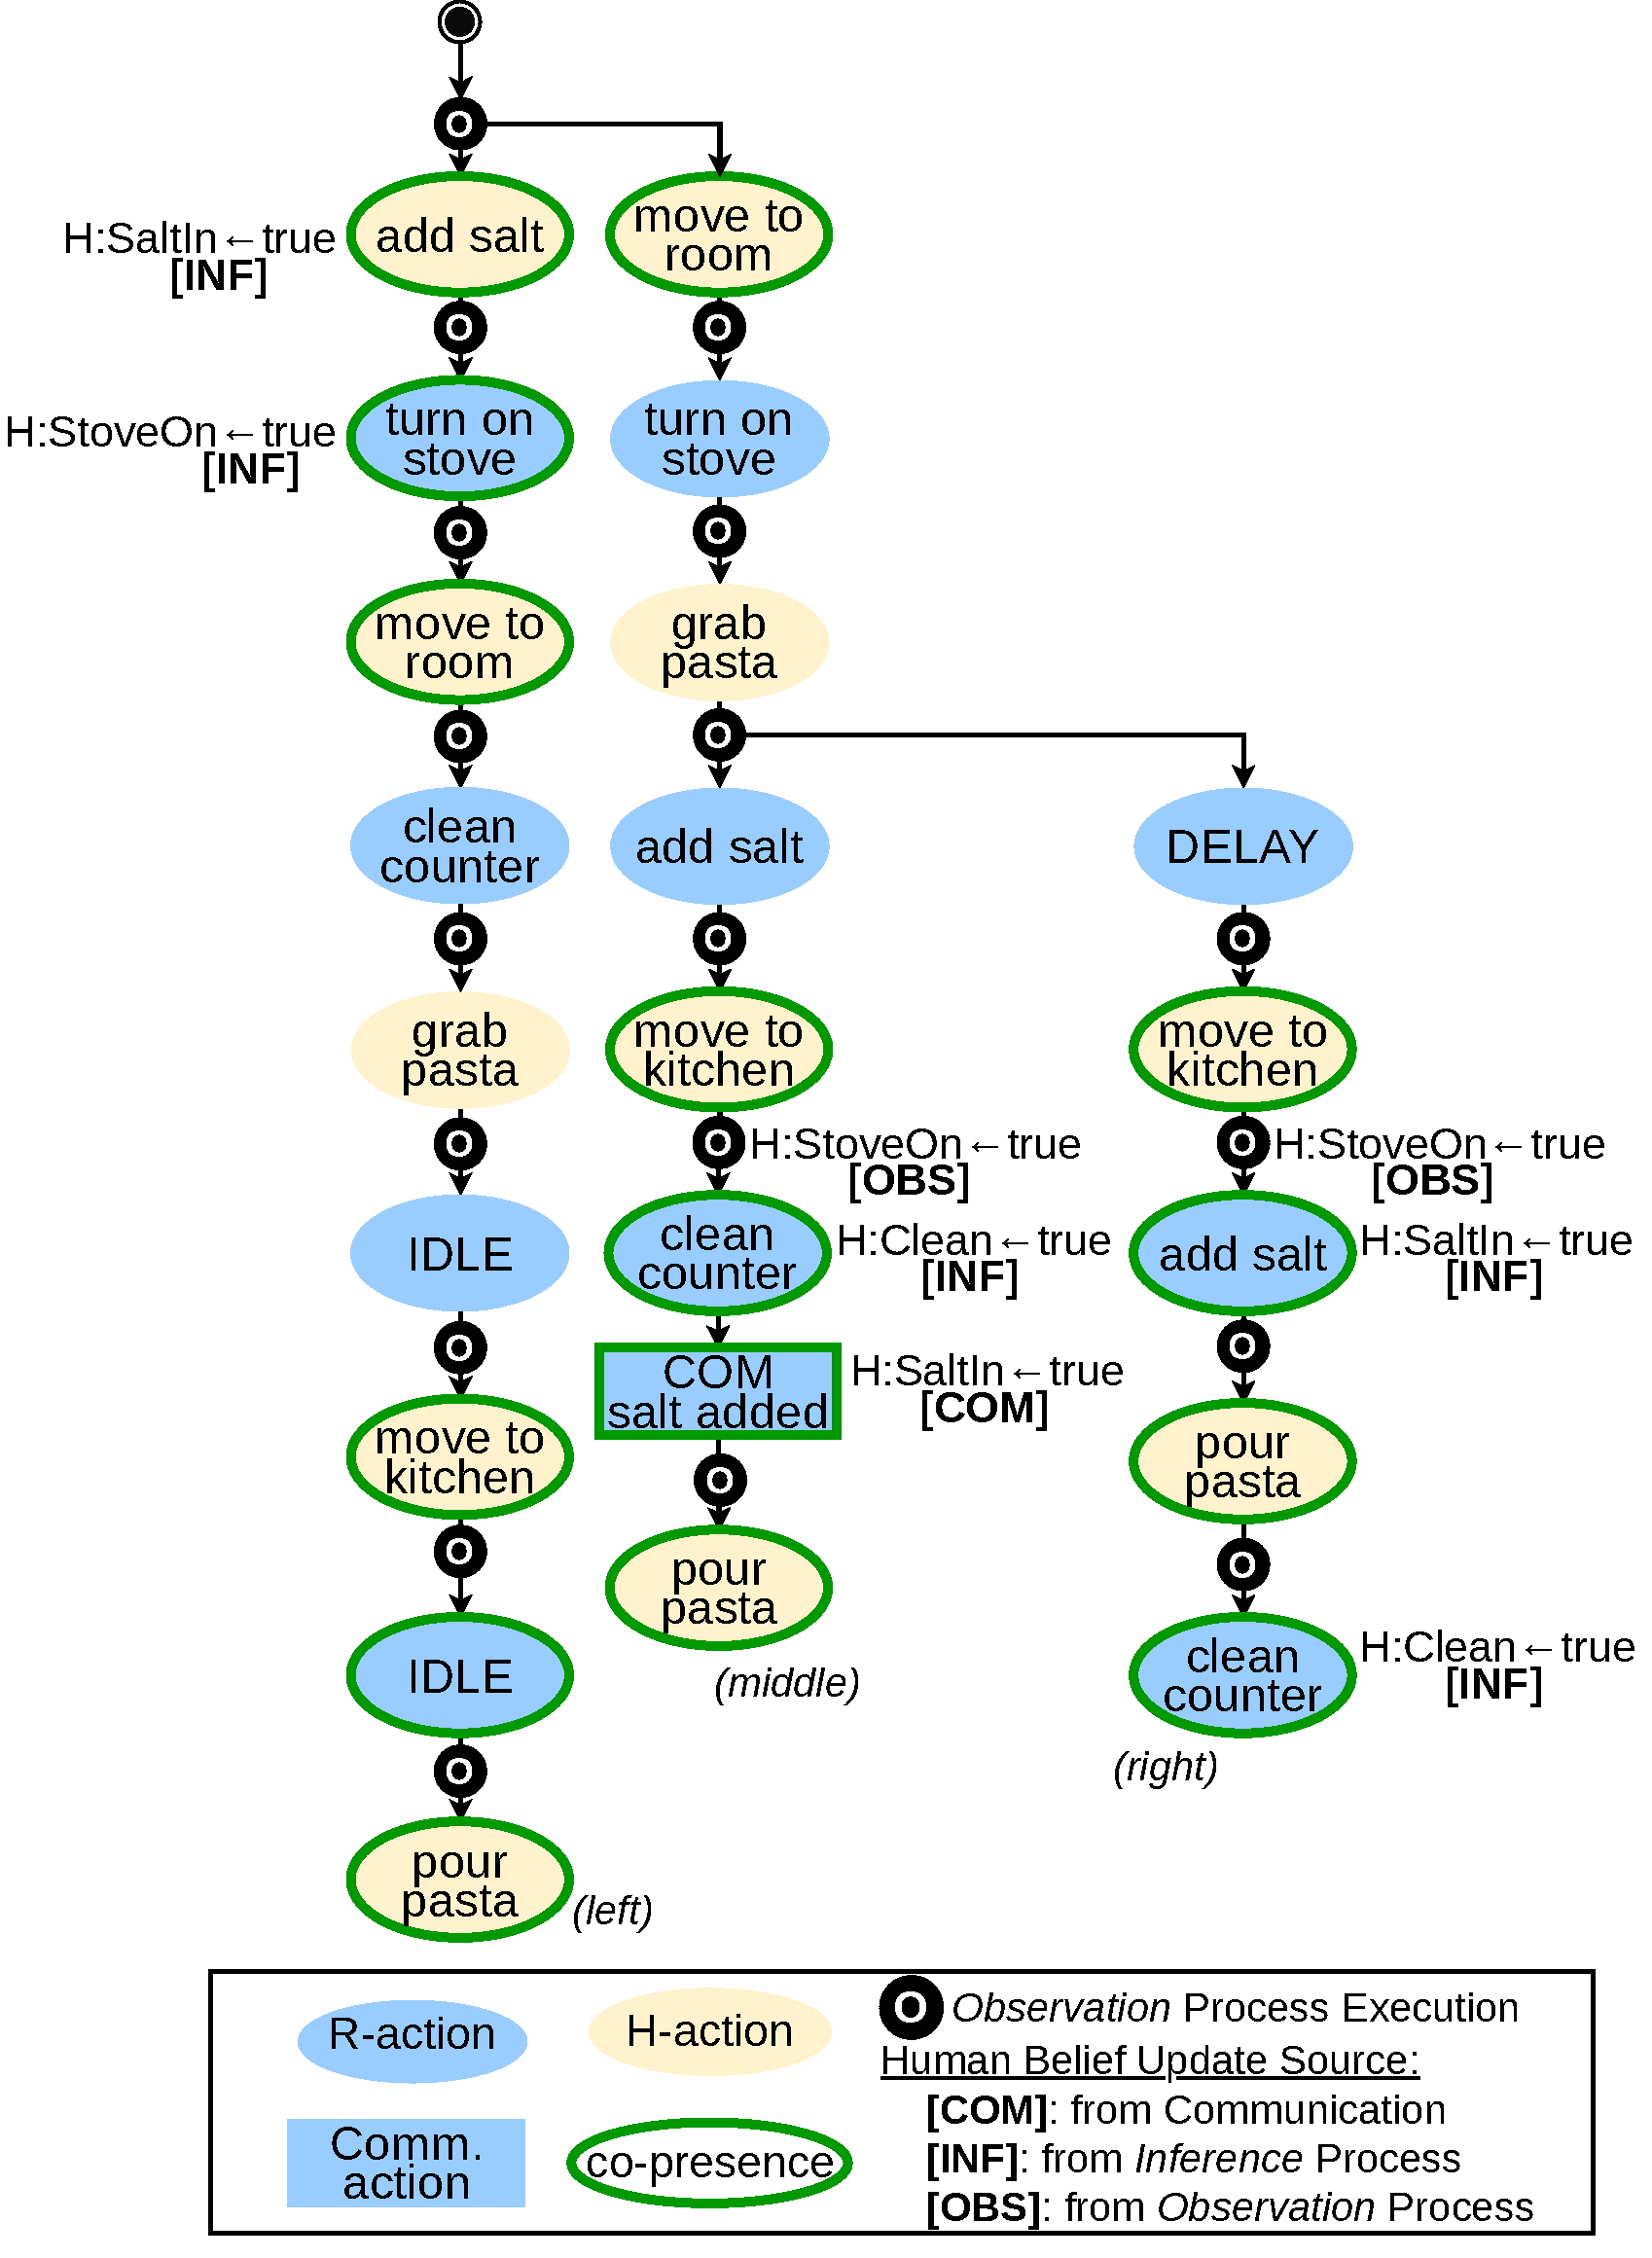
\includegraphics[width=0.65\linewidth]{images/Chapter3/plans.pdf}
    \caption{
    Plan obtained for the cooking scenario. 3 branches. Left: The human starts by adding salt. The only false belief is about \textit{``counterClean''} which is not relevant for the human agent, hence no comm is added. Middle: While the human is away the robot turns on the stove and adds salt, creating 2 false beliefs. 
    Once back, we estimate that the human agent
    will be able to assess the observable fact \textit{``stoveOn''} but not \textit{``saltIn''}. Since the human agent might add salt again due to this false belief, it is relevant and fixed with a communication action. Right: The relevant false belief about \textit{``saltIn''} is avoided by delaying the robot's action until the human is co-present.
    }
    \label{fig:cooking_plan}
\end{figure}

Considering the cooking domain, we discuss in detail the plans obtained with our approach to a problem corresponding to the description given in the introduction. 
I.e., there is no initial human false belief, agents both start in the kitchen, the pasta is in the adjacent room, the stove is off, and there is no salt in the water. The resulting plans are shown in Fig.~\ref{fig:cooking_plan} and their detailed presentation explains how the approach works in practice. 
Since human is uncontrollable and has different possible actions, the plan branches and the robot's actions are different in each case. 

In (\textit{left}) the human first adds salt and then the robot turns on the stove. In both cases, thanks to the inference process, we estimate that the human will be aware of both facts about the salt (\textit{acting}) and the stove (\textit{co-present}). Then while the human is away to fetch the pasta, the robot cleans the counter and since the human isn't co-present their beliefs aren't updated, containing now a false belief. Once back, since \textit{counterClean} is not \textit{observable} the observation process does nothing and the false belief remains. However, this false belief doesn't affect human actions (non-relevant), hence, there is no need to align human beliefs.

In (\textit{middle} and \textit{right}) the human first fetches the pasta by leaving the kitchen. Let's first focus on the (\textit{middle}) trace. The robot turns on the stove and adds salt while the human is away, creating two false beliefs. When returning to the kitchen, the observation process updates the human beliefs with the observable facts located in the kitchen. This fixes the false belief about \textit{stoveOn}. The robot then cleans the counter, observed by the human. 
However, without communication, the human's next action will be either ``add salt'' or ``ask the robot'', but considering the ground truth the human could directly pour the pasta. Hence, the false belief on \textit{saltIn} is relevant and has to be corrected. To do so a communication is inserted in the robot's plan and a ``delay'' branch is created (\textit{right}). 
In this delaying branch, the robot delays the add salt action until the human is co-present in order to make it observed (inference process) by the agent. 
In addition to this implicit communication, like in (\textit{middle}), the human assesses that the stove is on and hence can directly pour the pasta. 
\begin{table}[t]
    \centering
    \vspace{0.1cm}
    \caption
    {
    Success and communication ratio of different approaches. 
    }
    \label{tab:q_results}
    \begin{tabular}{@{}c|c c|| c| c@{}}
    % \begin{tabular}{c|c c|| c}
        \multirow{2}{*}{\textbf{Domain}} & \multicolumn{2}{c||}{\textbf{HATP/EHDA}} & \multicolumn{1}{c|}{\textbf{Only Comm}} & \multicolumn{1}{c}{\textbf{With Delay}}
        \\
        & \multicolumn{1}{c}{\textit{S}} & \multicolumn{1}{c||}{\textit{S I.Div.B.}} & \multicolumn{1}{c|}{\textit{Comm}} & \multicolumn{1}{c}{\textit{Comm}} 
        \\ \cline{1-5}
        \textit{Cooking}    &   18.6\%  &  6.9\%    & 69.5\% & 65.2\%\\
        \textit{Box}        &   25.0\%  & 14.3\%    & 79.7\% & 75.0\%\\
        \textit{Car}        &   12.5\%  & 0.0\%     & 68.8\% & 64.1\%\\
        \hline
        \textbf{Average}    &   18.7\%  & 7.1\%     & 72.6\% & 68.1\%\\
    \end{tabular}
\end{table}

\subsection{Experimental Results and Analysis}

In each domain, the actions and tasks remain the same. So here, a problem is defined by a starting agent ($R$ or $H$) and a pair of initial beliefs ($val^R_0, val^H_ 0$).
Initial ground truth ($val_0 \Leftrightarrow val^R_0$) is defined by setting each state variable to an initial value. But, 5 selected state variables can be set to 2 possible values instead of 1. Among these selected ones, 3 can diverge in human belief. This generates 256 pairs of initial beliefs where 12.5\% of them include initially aligned beliefs. Then, considering the starting agent, we obtain 512 problems for each domain. 
Each of the 1536 generated problems has been solved by HATP/EHDA, by \textit{our approach} using first \textit{only communication} and then using also \textit{delay}.
The obtained quantitative results appear in TABLE~\ref{tab:q_results}.
 
The overall success rate ($S$) and the one for initially diverging beliefs ($S I.Div.B.$) are shown for the HATP/EHDA solver. As expected, this solver always finds legal plans when dealing with initially aligned beliefs, but the low value of $S I.Div.B.$ reflects how poorly it handles belief divergences without specifically designed action models.
Our approach always finds legal plans so we omitted its success rates in the last two columns, and we can say that it solves a broader class of problems.

Furthermore, considering the initially diverging beliefs and the divergences created along the planning process, more than $87.5\%$ of all problems involve belief divergences. 
However, when using only verbal communication, only $72.6\%$ of the generated plans include communication actions.
This means that \textit{our approach} communicates only when necessary, and not systematically. 
The amount of communication is even reduced to $68.1\%$ when delaying actions. In the latter case, only delayed branches that do not imply the human to wait are kept. 

%%% SECTION %%%%%%%%%%%%%%%%%%%%%%%%%%%%%%%%%%%%%%%%%%%%%%%%%%%%
\section{Discussion and Limitations}

The underlying scheme allows just a single agent to execute a \textit{``real''} action at a time. 
However, a post-process can allow the execution of actions concurrently~\cite{CrosbyJR14}, however, note that the domain modeler has modeled $\mathcal{P}_{rh}$ as a sequential joint task. 
Parallelism is not considered in the current modeling and planning process, which limits the potential for concurrent executions. However, we are working on extending the framework to enable systematic planning with concurrent actions, aligning with~\cite{ShekharB20}.

We believe our modeling-level SA proposals could fit in any other planning approach framing multi-party systems having one controllable agent while can only hypothesize remaining agents' behaviors (e.g., human-centered AI).

Agents' SA models cannot simply refute a false belief, they can only assess new true facts to correct them.
E.g., assume the human \textit{wrongly} believes that the pasta is in \textsf{kitchen}. The SA does not help refute this when the agent is in \textsf{kitchen}
because appropriate knowledge reasoning w.r.t. \textit{NotAt(Pasta)} in \textsf{kitchen} is not taken into account.  
However, such issues do not affect the completeness and, if necessary, our approach \textit{tackles} such cases as relevant false beliefs.

We have planned a user study for the future to conform our framework with reality and validate the approach.

We discussed earlier that DEL knowledge representation is more expressive and flexible, and can handle uncertainty. However, it requires an augmented action schema to accurately maintain each agent's beliefs.
Think of a specification for \textit{``move''} action manually listing all the environmental facts to be observed by an agent for managing their beliefs. In our case, it is implicitly maintained within a state.

We can consider running a set of rules (e.g., \textit{graph-based ontology}) to bring new interesting facts in the state based on a set of known facts. We believe that this aspect opens up new possibilities in the future to integrate human-aware collaborative planning and ontology.

%%% SECTION %%%%%%%%%%%%%%%%%%%%%%%%%%%%%%%%%%%%%%%%%%%%%%%%%%%%
\section{Conclusion}

We propose an extension to a Human-Aware Task Planner called HATP/EHDA. 
The planner plans and implicitly coordinates the robot's actions with all estimated possible human (uncontrollable) behaviors that are then emulated to generate a new state.
Our extension and contribution are, first, to integrate a \textit{Situation Assessment} based reasoning system in the planner. This allows for maintaining distinct agents' beliefs based on what they can/should observe.
Compared to existing epistemic planners, this simplifies the action descriptions by focusing on their effects on the world, and not how they influence each agent's beliefs.
In addition, we propose to detect false human beliefs and tackle only the necessary ones in a principled way. First, we propose minimal and proactive explicit communication. Second, when pertinent, 
we propose an implicit communication by postponing the non-observed robot action until the human is co-present to observe it.  

The relevance of false belief, when to optimally communicate and parallelization are interesting future works, and we aim at conducting a user study to validate the benefits of the proactive robot behavior that our approach permits. 
\ifdefined\included
\else
\setcounter{chapter}{3} %% Numéro du chapitre précédent ;)
\dominitoc
\faketableofcontents
\fi

\chapter{Modeling and Planning for Concurrent and Compliant Joint Action Execution}
\chaptermark{Concurrent and Compliant Joint Action Execution}
\label{chap:4}
\minitoc

\chapabstract{This chapter presents my second main contribution, proposing a new human-aware task planning approach based on a step-based model of compliant and concurrent joint action. The approach's description is supported by empirical results proving its effectiveness in terms of the latitude of choice given to the human and the satisfaction of their internal preferences. We further validated this by developing an interactive simulator used for a user study, described in the following chapters.}

\section{Introduction}

\textit{From HRI paper}

In the context of HRC for a shared task~\cite{selvaggio2021autonomy}, we believe, based on the literature on joint action~\cite{sebanz_2006joint,sebanz-2009,clodic-2017,gordon-2023}, that the key towards a seamless interaction is, to consider the human as an uncontrollable agent and to be fully and concurrently compliant with them. 
The human should not be dictated which action they must perform, as in~\cite{roncone2017transparent,buisan_hatpehda_icra}, and the robot must comply with possible human decisions and actions during execution.

To collaborate with such humans with their (hidden) preferences, one can devise an online planning scheme coupled with a plan executor. 
However, in order to maintain real-time performance, online planning generally keeps a restricted horizon. 
Therefore, decisions taken online may lead to a dead end or may not lead to an optimal solution. 
Offline planning overcomes these issues. 

We propose a new \textit{offline} task planner which extends an existing human-aware planning system addressed in~\cite{buisan_hatpehda_icra}. 
The new planner is designed to take into account a \textit{Model of Execution}, which is in the form of an automaton and mainly inspired by the joint actions schemes. 
The model captures humans' latitude in their decisions. 
The planner's output is the robot's behavioral policy, which describes the robot's action in a state such that the action is congruent and compliant with the human's decision in this state and their (estimated) preferences, and that it is also legal to be executed in parallel. 
Our framework also allows humans to share their (new) preferences at any time during execution while the robot's policy is adapted online to that. 
In addition, our approach considers social signals to enhance execution by minimizing uncertainties. Both humans and robots issue signals to clarify situations such as performing an action, waiting for the other agent's necessary actions, or indicating a desire to remain passive.

In this chapter, we discuss relevant related work before describing the joint action model of execution that is central to our approach. 
We then describe the task planning problem and then introduce our novel framework. 
The following two sections to that, explain how the robot policy is generated by a three-step process: \textit{exploration}, \textit{characterization}, and \textit{generation}. 
We empirically evaluated our approach in simulation. With a BlocksWorld scenario, we show how our approach can effectively produce a concurrent robot behavior that is compliant with human online decisions and preferences.  

\section{Related works}

\textit{From HRI paper}

There have been a few attempts to cater to concurrent execution, but they deal with explicit time to manage concurrency~\cite{CirilloKS09a,kockemann2014grandpa}. 
In~\cite{CirilloKS09}, the robot does not plan actions for humans but forecasts their actions/plans from their activities and bases its own decision on the distribution of possible human plans. Here robots can perform actions concurrently, estimating/managing the completion time of the agents' actions carefully. 
We can see the human activity recognition part as a form of our \textit{identification (ID)} process of the automaton used. The robot needs such a plan/goal recognition technique to be compliant with the human's decisions. 
But, unlike ours, they do not consider an explicit shared goal among the agents, and hence humans are not concerned with stuff robots might be interested in during collaboration, e.g., giving signals to be passive. 
We believe that a shared goal creates a different context in HRC than the robot just being compliant with an estimated human's goals/plans. 
Moreover, we claim that dealing with concurrent actions is inevitable in planning even if actions are instantaneous, to effectively deal with multiple agent systems~\cite{CrosbyJR14,ShekharB20}, especially if there is a human operator involved like in our case. 
We extend HATP/EHDA~\cite{buisan_hatpehda_icra} to demonstrate that.

In another work, both \textit{recognition} and \textit{adaptation} take place simultaneously and comprehensively~\cite{levine2014concurrent}. 
It deals with action scheduling of an already generated contingent plan comprising human's and robot's actions. 
It outputs schedules for the robot actions that can execute concurrently but to do that explicit temporal constraints are considered. 

Ramachandruni, Kent, and Chernova (2023)~\cite{RAMACHANDRUNI2023} propose a communication free human-robot collaborative approach for an adaptive execution of multi-step tasks. 
In their approach, the robot observes and supports human decisions, actively selecting actions to optimize collaborative task efficiency. 
Unlike our approach, they introduce an extended collaborative HTN representation with role assignment for planning and state tracking during execution, which is more in line with~\cite{roncone2017transparent}. 
In contrast, we employ two distinct HTNs for robot and human capabilities and use an AND/OR tree for exploration and execution tracking. While their online planning may enhance scalability, optimality is not guaranteed. 
Also, our scheme accommodates both verbal and non-verbal communication, allowing the human to express preferences that update the robot policy online. 

\section{Model of Concurrent Joint Action Execution}

    \subsection{Rationale and Example}



Our task planning approach uses a model of execution to improve the fluency and amenability of HRC. 
This model is in the form of an execution controller and is based on several key notions and mechanisms borrowed from studies on joint actions~\cite{Sebanz_2016,kourtis2014attention}, and adapted to Human-Robot Joint Action~\cite{clodic-2017,curioni-2019}.
The key idea is that co-acting agents co-represent the shared task context and integrate task components of their co-actors into their own task representation~\cite{Schmitz-2017, Yamaguchi-19}. Also, coordination and role distribution rely strongly on reciprocal information flow, e.g., social signals~\cite{curioni-2019}, prediction of other's next action~\cite{luke-2018}.

Our proposed execution model is implemented on a robot that co-acts with a human, integrating explicit representation and exploration of the task representations for the robot and for the human. 
It also identifies precisely how reciprocal information flow is used in task execution (detecting and interpreting human actions, signals produced by the robot while acting, and also when the robot waits for human actions or their signals).

Another essential question is the criteria for choosing the next action, or more globally, how to share the load between the two co-actors. The choice depends on the context and actors' preferences~\cite{Gombolay-2015, Strachan-2020, Curioni-2022}. 
Concerning the case when one actor is a robot, we think it is important to provide a standard default behavior of the robot where the robot does its best to reduce human load but still leaves full latitude to act whenever humans want. 
Our scheme provides this ability and also allows humans to inform about their preferences at any moment.

\begin{figure}
    \center
    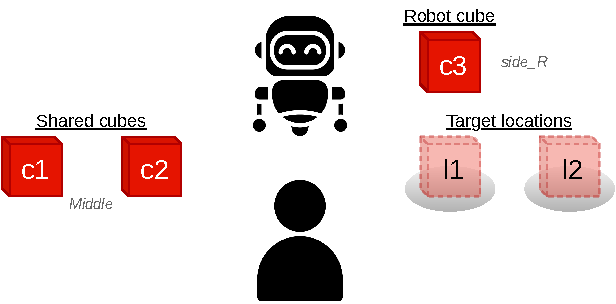
\includegraphics{Chapter4/example_conflict_pick.pdf}
    \caption{Example of conflict for a concurrent joint action. 
    Shared cubes, \emph{c1} and \emph{c2}, can be picked up by both agents and only the robot can pick \emph{c3}. 
    Agents can simulateously pick up both shared cubes, but they must coordinate their actions otherwise they might conflictingly try to pick the same cube. 
    Similarly, another coordination is required to avoid placement conflicts between locations \emph{l1} and \emph{l2}.
    However, notice that the robot can pick \emph{c3} without any risk of conflicts with the human action.}
    \label{fig:conflict_pick}
\end{figure}

To better understand the problem we are trying to solve, let's consider an example where concurrent agent's actions can be conflicting. This example consisting in a simple pick and place task is depicted in fig~\ref{fig:conflict_pick}. The human and the robot have to pick cubes, \emph{c1} and \emph{c2}, that both can reach. 
The cubes can be picked up simulateously unless the agents try to pick the same cube, which causes conflicts between their actions. As a result, despite being executable in parallel, the actions are interdependent. Thus, the agents must coordinate their actions for a smooth execution.
A similar coordination must happen when placing the cubes to avoid conflicts between \emph{l1} and \emph{l2}.
However, a third cube \emph{c3} is present and can only be picked up by the robot. The robot can pick \emph{c3} without any risk of conflicts with the human action. 

This example illustrates the need of coodination even for simple tasks. It also shows that considering possible conflicts can also be a criterion to optimize. Thus, the best robot action might be to pick up \emph{c3} instead of one of the shared cubes to avoid potential conflicts, even if \emph{c3} is more distant and more costly to pick than \emph{c1} and \emph{c2}.
This example also highlight the relevance of exploring several possible executions of concurrent actions while planning to anticipate and evaluate such situations and produce a robust, compliant and efficient robot policy. This is why, based on joint action literature, we formulated a model of concurrent joint action execution described below that will guide our planning search.

\subsection{Abstracted Joint Action Model for Planning}

\begin{figure}
    \centering
    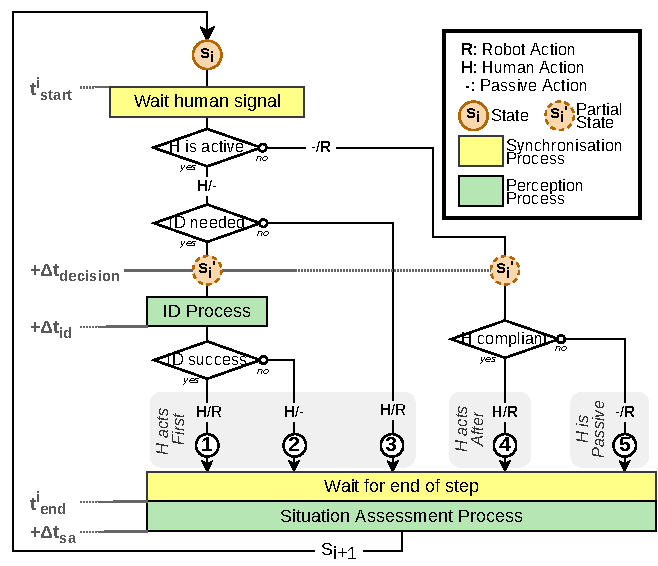
\includegraphics[width=0.8\linewidth]{Chapter4/simplified_automaton.pdf}
    \caption{
    Abstracted Model of Execution in the form of an automaton run by the robot. It captures the latitude of uncontrollable humans in their actions and guides our task-planning approach.
    In this paradigm, the two agents can act concurrently but one is always compliant with the other's decision to act.
    Here, the human is always free to decide whether to start acting first, or after the robot, or not to act at all.
    To be compliant, the robot attempts to identify human decisions using perception and situation assessment as well as possible collaborative human signaling acts (e.g., gestures or speech).
    }
    \label{fig:simplified_model_exec}
\end{figure}

% Full page figure formats w/r line of caption:
% - 5 lines = 210x294 ratio
% - 4 lines = 210x301 ratio
% - 3 lines = 210x308 ratio

The model of execution we formulated, depicted in fig~\ref{fig:simplified_model_exec}, is inspired by joint action literature and describe the agent's coordination during execution. It comprises synhcronisation and perception processes based on social signals exchanged between the agents such as starting an action (arm motion), hand gestures, or verbal communication. In this section is presented a simplified and abstracted version of this model that suffice to guide our planning framework. A complete version which explictely models the human behavior and exhanged signals is provided in the next chapter and used to supervise the execution of the produced robot policy.  


% \textbf{TODO: add numbered marks in the figure to refer to easily for description, also describe the conditions: H is active, etc...}

The model describes the possible transitions from a given state to another, step by step. The robot always informs the human about the beginning of a step and then wait for their decision by looking at social cues. This waiting process is represented by the top yellow rectangle in the figure. This human decision can either be to start acting or to be passive. Hence, the robot always let the human first decide which action they want to perform, including the choice to be passive. This decision is detected with perception by tracking social cues such as human motions and hand gestures.

The diamond shapes below the first synchronization process are conditions, driving the automaton into different branches depending on specific conditions. First, we differenciate the cases where the human is passive or not (``H is active''). 
Ihe case where the human is performing an action, the `yes' branch, we first check if the human action must be identified or not. Indeed, so far only the fact that the human is acting is known, but not yet which particular action they are performing. 
To avoid potential conflicts, we consider that there is no need to identify the human action if the best robot action does not depend on the human decision. For instance, consider in the cube picking example presented in figure \ref{fig:conflict_pick} that the cube \emph{c3} is easier to pick and place for the robot than the two other one. Thus, regardless of which cube the human picks, the robot should pick \emph{c3}, its best action does not depend on the human decision. In such case, there is no need to idenfiy their action. However, if \emph{c3} is effectively harder to place than \emph{c1} and \emph{c2}, the robot must first identify which cube the human is grabbing to pick the other one. As a result, the model differenciate the cases where the human action must be identified (``ID needed'') or not. If not, then the robot can directly start acting (branch 3). Otherwise, the Identification (ID) process is executed and may either be successful (``ID success'') or not. If not, to avoid any potential conflict, we decided that the robot should remain passive (branch 2). If the human action has been successfully identified then the robot can perform concurrently the best corresponding action (branch 1).

In the case where the human decided to be passive, the robot should start acting. 
However, while the robot is acting, we consider that the human is free to either remain passive until the next step (branch 5) or to ``change their mind'' and start acting (branch 4).
This is represented by the diamond shape ``H compliant''. In the case where the human decides to start acting after the robot started, the human can only perform actions that are not conflicting with the already started robot action. Note that this case can be seen as a way for the human to let the robot decide and then comply with the robot's decision. Still, the human decided to let the robot decide, thus, the human is given as much latitude of choice as possible.

Overall, at every step of the execution, the human is free to decide: 1) to start performing any feasible action, the robot will comply with this decision; 2) to let the robot decide and act first, and then purposely we compliant with the robot; 3) to be passive and let the robot act alone.

When both agents finish their actions, the step is considered as \textit{``over''}. This synchronization is represented by the bottom yellow rectangle ``Wait for end of step''. Then, a Situation Assessment Process is executed to assess the new world state ($s_{i+1}$), which is the result of the concurrent actions being executed in the state $s_i$. Once the next state is identified, the automaton repeats until the task is solved and a goal state is reached.

Note that if for any reason both agents are passive during a step, then the state is unchanged and the step is repeated. 

%%%%%%%%%%%%%%%%%%%%%%

% Let's describe this simplified model in the form of an automaton on which on planning algorithm is based on.
% In a state, a human decision can result in one of three outcomes.
% First, the human can choose to act first (\textit{left~subtree}).
% If the robot's best action is not in conflict with the human action (e.g., \textit{pick~C}), the robot can safely perform this action concurrently with the human operator (\textit{branch~3}).
% However, if the robot's best action is either \textit{pick~A} or \textit{pick~B}, the human action must be identified first with a subroutine in order to be compliant with it.
% If this subroutine is successful the robot can perform any action which is congruent with the identified human action (\textit{branch~1}). 
% This includes the robot's choice to be \textit{passive} and let the human act alone. 
% However, if the robot is unable to identify the human action, it must remain passive in order to avoid potential conflicts (\textit{branch~2}). 
% Then, the human can either decide to be \textit{passive} or to act after the robot (\textit{right~subtree}). 
% In both cases, the human is \textit{passive} at the beginning, making the robot to start performing alone a feasible action. 
% While the robot is acting, the human is free to remain \textit{passive} until the next step (\textit{branch~5}) or to choose a congruent action to act concurrently (\textit{branch~4}). 
% As a result, the human can always choose to 1) act first, 2) act after the robot, or 3) not act at all. 
% The robot will always be compliant with these online human decisions.

% When both agents finish their actions, the step is considered as \textit{``over''}. 
% Then, another subroutine assesses the new world state ($s_{i+1}$), which is the result of the concurrent actions being executed in the state $s_i$, before repeating the whole process until the task is solved.

% Note that if both agents are passive (the human decides to be passive when the robot cannot act) then the step is repeated. 

\section{Problem specification + solution}

    \subsection{Problem}

Belief divergences are out of the scope of this particular work. Hence, for simplicity reasons, we consider the two beliefs (robot and estimated human ones) as always aligned, and they are represented as a unique world state. However, we are convinced that this work could be adapted easily to consider the two distinct beliefs.

The problem is specified as shown here \ref{sec:problem_spec} in Chapter~\ref{chap:2}. For simplication purposes, in this contribution, no belief divergence are considered. Therefore, the two agents beliefs are always aligned and initialized with a same initial world state using state variables. Then, distinct human and robot action models are described with HTNs and distinct human and robot initial agendas are provided comprising a shared task to accomplish. 

\subsection{Solution}

\begin{figure}[h]
    \centering
    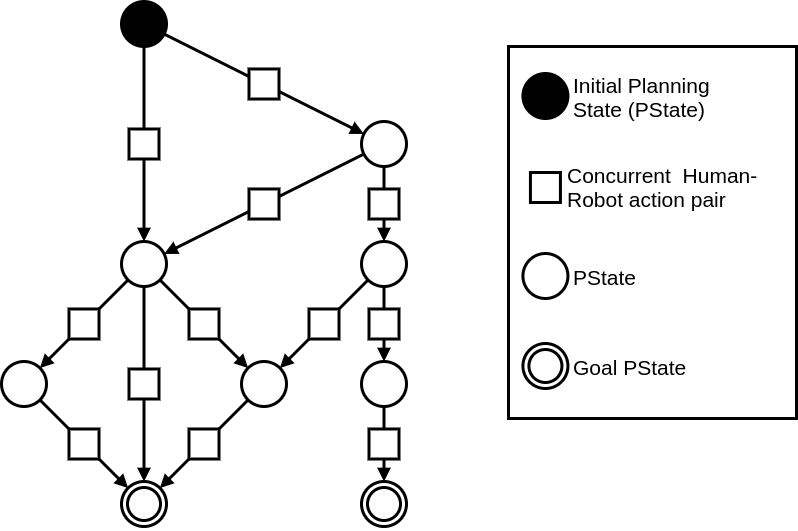
\includegraphics[width=0.7\linewidth]{Chapter4/solution_graph.png}
    \caption{Directed acyclic solution graph}
    \label{fig:solution_graph}
\end{figure}

A Planning state, referred as p-state, corresponds to a state in which the planning problem is while progressing toward a solution. A p-state contains the current world state (aligned beliefs of the agents) and the respective agenda of the human and the robot. Thus, keep in mind that p-states are very different from world states.
The initial p-state is formed using the initial human-robot agendas and the initial world state given in the problem specification. P-states are connected with each other through concurrent pairs of human-robot actions. Note that we consider passive actions, hence, there may be only one active agent in a pair if concurrent human-robot actions. A goal p-state is characterized by a world state satisfying given goal conditions and by empty agendas.
The exploration produces a Directed Acyclic Graph (DAG), referred as the search graph, from the initial p-state to several goal p-states through sequences of concurrent action pairs. Thus, any path from the root to a leaf is a possible plan. Once the exploration done, search graph computed, another process extract the optimal robot policy from the graph. In the manner of an AND-OR tree, this policy indicates for all p-states the best concurrent robot action (OR node) to execute to be compliant with any possible human action (AND node).


Clarification of the directed acyclic graph. Nodes represent p-states and are connected with each other through directed edges representing human-robot concurrent action pairs. However, for practical reasons action pairs are considered as nodes of the graph having only one parent p-state node and one child p-state node. Consider that each directed edge between two p-state have one unique intermediate action pair node. The graph has one root node (no parent) which is the initial p-state. All leaf nodes (no children) represent a goal p-state. 

It is one of our design choice to do not consider explicit action costs and perform an exhaustive offline search to produce this search graph in order to solve a problem. Since the policy generation is very quick it allows generating and updating the robot policy online according to human feedbacks. 


\begin{figure}
    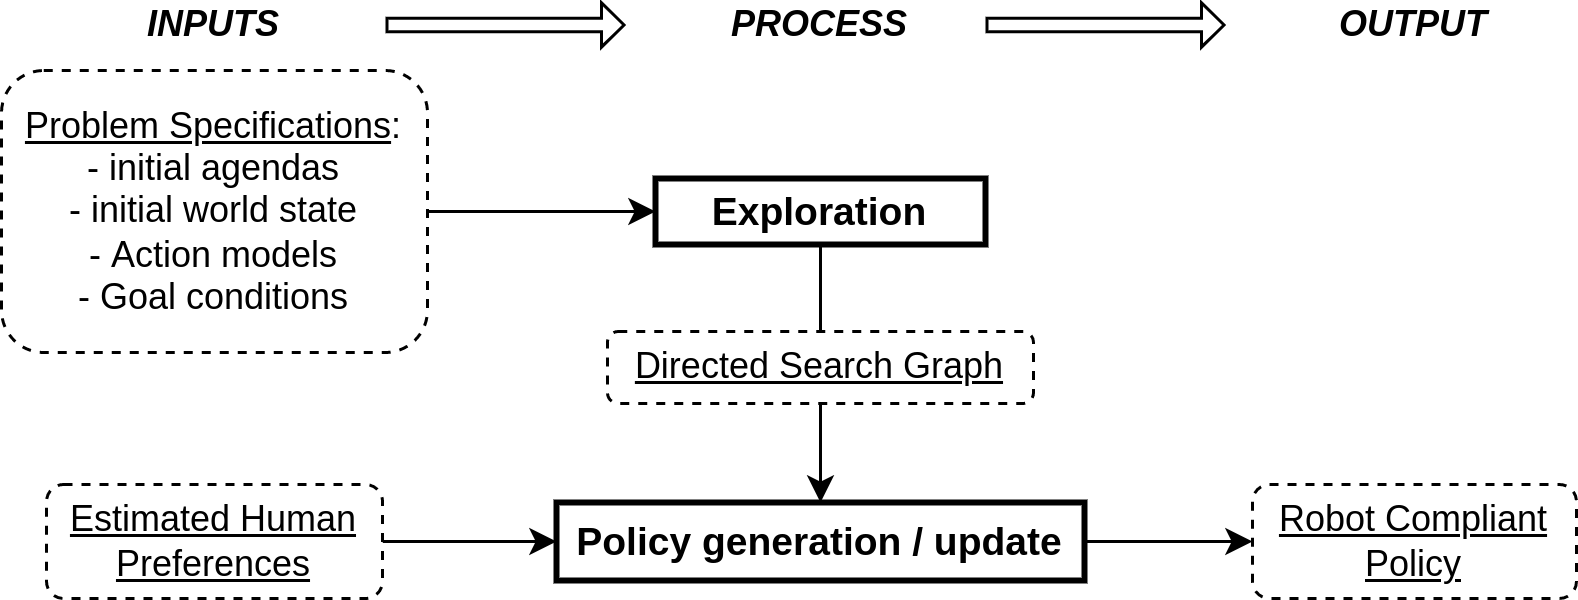
\includegraphics[width=\linewidth]{Chapter4/overall_process.png}
    \caption{Overall planning process}
    \label{fig:overall_process}
\end{figure}

\section{Exploration}

This section details how the exploration happens, and thus, how the search graph is generated. This requires several sub-process which are each detailed here. First, the overall exploration process is presented, and next subsections provide details on the sub-processes mentioned in the overall process.

    \subsection{Overall process}

We keep track of the p-state to explore, and this set is being initialized with the initial p-state. Then, until the set is empty we select one and explore it.
First, from this selected p-state, every possible concurrent human-robot action pairs are computed considering both agendas, the world state and reasoning on the compatibility of the actions in terms of preconditions and effects. This process requires several sub-steps and is detailed later. Thus, we obtain several action pairs leading to the same amount of new p-states (with updated world state and agendas).
Second, we check if any of the newly created p-state are similar to any existing p-state. If so, we can "merge" them to avoid redundant computations. To do so, we basically keep track of the unique p-state already checked and for each new p-state we check if it is similar to one of the already checked one. 
If not, the new p-state is added to the set of already checked p-states. 
If a similar one is found, the new p-state is deleted and the action pair leading to it is connected to the existing p-state instead.
Eventually, the remaining new p-states are added to the set of p-states to explore. 
When the set of p-states to explore is empty then the exploration is over and the graph obtained corresponds to the "search graph" where any path from the initial p-state to a leaf corresponds to a possible execution trace / plan.

    \subsection{Compute next agent actions}

From a p-state, more precisely from a world state and an agenda, we can estimate what are the next action an agent is likely to perform. Doing so is referred as the refinement process. To do so we use the corresponding action model in the form of an HTN. Here the agendas are considered as list of abstract or primitive task, where primitive task can be executed (actions), and abstract ones can be decomposed into several others subtasks. 
The refinement process consists in applying applicable methods of the first task of the agenda until it is primitive. When several methods are applicable they are all applied in a distinct refinement trace.
Eventually, for each different sequence of applied method we obtain a new agenda starting with a primitive task. For each such primitive task we create a copy of the world state contained in the given p-state, and we applied the correspond action, updating the world state. 
Hence, for each possible action a new p-state is created with the refined agent agenda, the unchanged other's agenda and the updated world state. 
Note that this process can "generate" default passive actions in several cases. First, when an agent's agenda is empty an \textit{IDLE} passive action is inserted as the first primitive task in the agenda. This means that the agent has nothing to do and thus is likely to remain passive. Either when there are no applicable methods or when the primitive task is not applicable then a \textit{WAIT} passive action is inserted. This means that the agent has still something to do but cannot do it currently. Note that when computing the concurrent pairs of action we also add the \textit{PASS} action which corresponds to the agent being voluntary passive, despite having something to do. Note also that these different passive action types just help to better understand the generated plans, but they are treated equally / similarly in the planning process.

    \subsection{Concurrent action pairs computation}

This sub-process computes from a given p-state all possible concurrent action pairs that may be executed. It is based on the previously described refinement process. This main objective of this sub-process is to identify the next actions the agents are likely to perform to reach the goal and identify which of them can be executed in parallel. The classical way to do such reasoning is by analyzing the preconditions and effects of the two actions and determine if there are conflicts between them, e.g., the effects of the first action makes the preconditions of the other false.
However, our current python implementation of the planner is convenient but has no "explicit" preconditions and effects. Everything is defined through python function. The effects of an action are a function with a world state as input and returns the updated world state. Action preconditions are functions with a world state as input and return a boolean. And methods (of an associated abstract task) are functions with world state as input and return a list of tasks to update the agenda with. Methods also have preconditions working similarly then action preconditions. 
Hence, it's challenging to extract the explicit effects and preconditions of an action. That is why we decided to rely on an assumption to check the compatibility of concurrent actions. 
We consider the following in a given state. 
If action 1 and action 2 can be sequentially performed in both orders (1$\rightarrow$2 and 2$\rightarrow$1). Then we can assume that there are no causal links between the two actions and that they can be performed concurrently. The only care to take are shared resources such as a tool that would only be used during the action, making it available before and after but not during the action. To tackle this issue, shared resources are explicitly declared in the world state and in the action models. Two actions requiring a same shared resource cannot be parallelized.
One benefit the way we check if two actions are mutually exclusive is making the actions estimations a black box. Indeed, we can easily replace the way we estimate the next actions each agent is likely to perform. Especially for the human, we could use a pretrained human activity estimator neural network, or more classical planner like PDDL. 

With the causal principle above in mind, we proceed as follows to compute the possible concurrent action pairs from a given p-state. We start by estimating all possible human actions by refining the human agenda, generating a new p-state for each possible action. For each such p-state we first create an action pair where the robot is passive by inserting a \textit{PASS} robot action. This \textit{PASS} pair is stored among all other "human pass pairs". Second, we refine the robot agenda to obtain all feasible sequences of human then robot actions and their associated p-states. We refer to them as the sequential human starting pairs. In a symmetrical way we compute the sequential robot starting pairs and "robot pass pairs" by starting with the robot then refining the human agenda.

Eventually, every action pair which is present in both the human and robot starting pairs are extracted and added to a set of concurrent action pairs. 
Additionally, here passive action are always parallelizable. Indeed, the only case where this couldn't be the case is when considering "joint actions" requiring the two agents such as lifting a table/object together. For now, such actions are not considered. Thus, the two sets of \textit{PASS} pairs are directly added to the set of concurrent action pairs. 
Lastly, a double passive pair with two PASS is generated and added to the concurrent set. This pair is special since it doesn't update the world nor the agendas, hence, it leads back to the previous p-state without progressing toward the goal. These pairs not need to be explored and help it different ways. First, it helps the execution for instance when only the human can act but decides anyway to pass voluntary. Then the policy will natively stay in the same p-state. Second, it is easy to detect dead-ends which correspond double \textit{WAIT} pairs. In such case, both agent cannot act, due to the lack preconditions for action or decomposing an abstract task, and they remain stuck without solving the task.  
Last, double \textit{IDLE} pairs indicates that both agendas are empty and thus that the task should have been solved. 

The obtained set of concurrent action pairs corresponds to all possible concurrent action that the human and the robot can execute in parallel in the initially given p-state. Each possible pair leads to a new p-state with updated agendas and world state, creating a tree structure. 

    \subsection{Merging p-states}

Although the tree structure produced by the process described above is complete and sound, it is inefficient and scales badly. Indeed, during the exploration we are likely to encounter several times similar p-states. For instance, consider an action pair where both the human and robot are active leading to a new p-state, one branch. Now, consider a first action pair where only the human is active, and a second where only the robot is active. Performing those two last pairs in both orders creates two other branches. However, even though the trace is different, the three p-states are identical (same world state and agendas) and it's highly redundant to explore independently each of them. That is why after each computation of the concurrent action pairs we check if any of the newly generated p-state is similar to an existing one, and if so, we connect the corresponding pair to the existing p-state to avoid redundant explorations. Doing so we transform the tree structure into a directed acyclic graph (on the condition that we don't consider double \textit{PASS} cycles). In the manner of a tree, we will refer to nodes without child as leaves nodes, which are goal p-states. Hence, now, each leaf can be reached with several paths. 
When looking for similar existing p-state, we assume that p-states which are parent with the new p-state, directly of not, will necessarily be different, and thus they are excluded. This speeds up the comparison process. 

\section{The Robot Policy}

First of all, as depicted in figure~\ref{fig:and_or}, all children concurrent action pairs of a p-state ($PS / ps_i$) can actually be seen as an AND-OR graph. Since we want to preserve the latitude of choice the human have at execution, each possible human choice of action is considered as an AND edge and leads to a partial p-state ($PS' / ps_i^j$). And from a partial p-state, each compliant concurrent robot action is considered as an OR edge and leads to another p-state.

Notations: A p-state is referred to as $ps$, and $ps_i$ is the $i$-th p-state. A partial p-state is referred to as $ps'$ and $ps_i^j$ is the $j$-th partial p-state of the $i$-th p-state.

Thus, generating the robot policy $\Pi$ consists in identifying the best concurrent compliant robot action $RA^*$ for each possible human action, or partial p-state $ps_i^j$.

These best concurrent robot actions are determined by aiming to optimally satisfy an estimation of the human preferences regarding the task. Eventually, at execution, the human is free to perform any of the explored action and the robot will accordingly perform an optimal concurrent action to both solve the task and satisfy their estimated preferences.

Hence, before giving more details about the policy itself, we first describe the format of human preferences, how we could estimate them, and what it allows us to do. After, we describe the actual process to generate the robot policy from the search graph using the estimated human preferences


**The robot policy consist in performing the best robot action according to the node and the human action, i.e., robot action stored in the "best compliant" pair corresponding to the human action.
If all "best compliant" pair have the same robot action, the robot can perform as soon as the step stars, otherwise the human action must be identified.**

\begin{figure}
    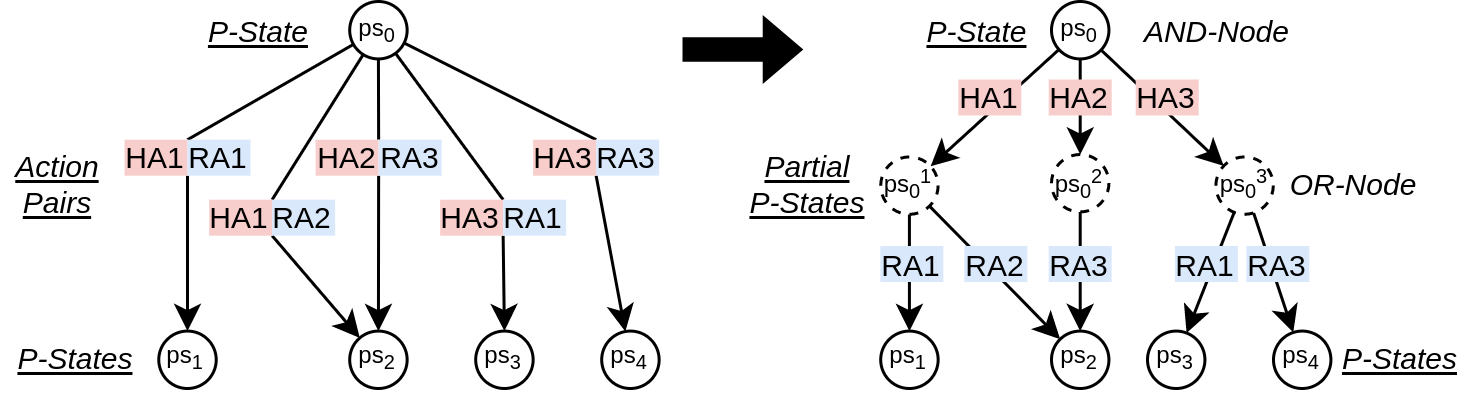
\includegraphics[width=\linewidth]{Chapter4/and_or_tree.png}
    \caption{AND-OR graph representation of the action pairs. 
    The robot policy must be compliant to any decision of the human. Hence, the problem can be seen as an AND-OR graph where for each possible human choice of action (AND node), we must determine the best concurrent robot action among the possible robot actions (OR node).
    }
    \label{fig:and_or}
\end{figure}


    \subsection{Estimated Human preferences}
estimations, format, Discussion(often inaccurate, hence our Approach), consider metrics, is a prioritized sequence of metrics to max or min, allow comparison of metrics

In this approach, instead of trying to minimize action and social costs, which are challenging to estimate accurately and quantitatively, we decided to aim at satisfying an estimation of the human preferences. In a way, the costs are included / covered / reflected in the human preferences. Our approach is to characterize each possible trace with a set of various metrics such as follows:

\begin{itemize}
    \item \textbf{Time of Task Completion}: Time step at which the task if achieved.
    \item \textbf{Time of End of Human Duty}: Time step after which the human can remain passive.
    \item \textbf{Human Effort}: Number of non-passive human action.
    \item \textbf{Global Effort}: Number of non-passive human and robot action.
    \item \textbf{*Passive While Holding}: Number of steps where an agent is passive while holding a cube.
    \item \textbf{*Number of Drop}: Number of times an agent drops cube (place back a cube on the table, not in the stack).
\end{itemize}

Note that general metrics are complemented with additional domain specific metrics (marked with a star *), given in the problem specification. The set of metrics helps to characterize and evaluate each possible plan / trace. However, even if the possible plans are characterized we so far have no way to compare them and find the best one. Doing so requires additional criteria indicating how to prioritize and compare the different metrics.

That's where we consider an estimation of the human preferences to allow us to the plans and which are given by any mean external to our system. The preferences can be estimated or also given, verbally or not. Here, we consider the human preferences in the following form. These preferences are an ordered list of the metrics characterizing the traces. Note that it's not necessary for all metrics in the list above to be present, but only them can appear in the preferences. This ordered list indicates if each metric should be maximized or minimized, and in which order / with which priority. For instance, assuming the preferences aim to minimize all metrics, the best of two given plans is the one with the lowest first metric of the list. If the two plans have equal first metric then we use the second metric, and so on. Here are two arbitrary examples of human preferences trying respectively to finish the task as fast as possible and to minimize the human effort (all metrics are minimized):

TTC - GE - HE - TEH - PWH - ND 

HE - TEH - TTC - GE - PWH - ND 

Note that estimating either human preferences or explicit action and social costs is challenging and is hardly accurate, those are very context dependent and can even vary over time.
Being aware of this, we use the estimated human preferences as a guide for the robot behavior, but we also make sure to be compliant to the human activity to lessen the impact of a wrong estimation. 

    \subsection{Generation}

\begin{figure}
    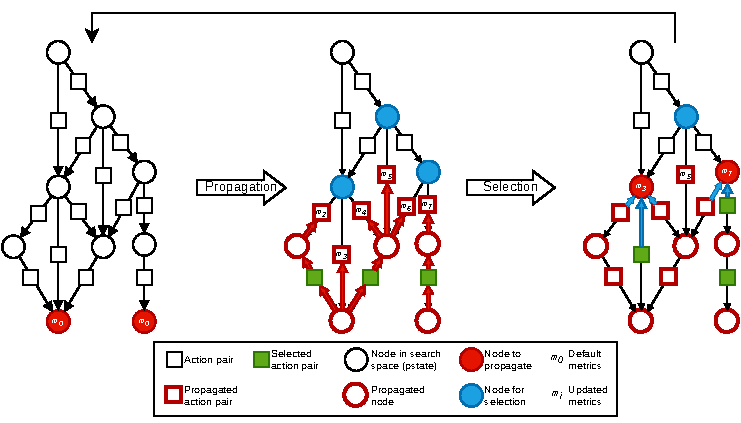
\includegraphics[width=\linewidth]{Chapter4/policy_generation.pdf}
    \caption{\textbf{TODO: show metrics in branches? just small $m_i$ in each branch?} Policy generation process illustration on an arbitrary search graph. Propagation and Merge processes repeat until there are no more p-state/node to propagate nor for selection.}
    \label{fig:policy_generation}
\end{figure}

To generate the robot policy $\Pi$ from the search graph we proceed from the leaves to the root. 
Overall, we progressively compute the set of metrics for each possible trace. When reaching a p-state with several children we compare the metrics of the different traces leading to this node. We are then able to identify the best trace leading to each partial p-state, and the best trace leading the p-state. Each best trace to a partial p-state is used to update the robot policy, and the overall best trace is used to continue propagation the best reachable set of metrics.
This process is achieved by repeating two sub-routines detailed just below, namely: Propagation and Selection. 

\begin{algorithm}
\caption{Policy Generation}\label{alg:policy_generation}
\begin{algorithmic}[1]

\State \textbf{input}: $leafNodes$ \Comment{Set of all leaf p-states from the search graph}
\State $psToPropagate \gets \emptyset$
\State $psForSelection \gets \emptyset$

\State $Initialization(psToPropagate, leafNodes)$

\While{ $psToPropagate \neq \emptyset$ and $psForSelection \neq \emptyset$ }
    \State $Propagation(psToPropagate, psForSelection)$
    \State $Selection(psToPropagate, psForSelection)$
\EndWhile

\end{algorithmic}
\end{algorithm}

    \subsubsection{Format and Initialization}

During this process we compute and store the best reachable set of metrics alternatively in the p-states and in the action pairs. Initially, we store default/null metrics in every leaf p-state. Then we keep track of two types of nodes. First, keep track of the nodes which metrics should be propagated in the next step, those are stored in the set $\{psToPropagate\}$ which is initialized with all leaf p-state nodes. This set is later populated by the Selection sub-routine. Secondly, we keep track of the nodes to that should select among several the best set of metrics, and thus, the best actions to perform. This set is $\{psForSelection\}$ and later is populated by the propagation sub-routine while being emptied by the selection sub-routine. The process is over when the two sets are empty, thus, when they are no more nodes either to propagate nor for selection.

% The default metrics are the following:
% \vspace{-\topsep}
% \begin{itemize}
%     \setlength\itemsep{-0.3em}
%     \item \textbf{Time of Task Completion} $= -1$
%     \item \textbf{Time of End of Human Duty} $= -1$
%     \item \textbf{Human Effort} $= 0$
%     \item \textbf{Global Effort} $= 0$
%     \item \textbf{*Passive While Holding} $= 0$
%     \item \textbf{*Number of Drop} $= 0$
% \end{itemize}

    \subsubsection{Propagation}

The propagation sub-routine is depicted in algorithm~\ref{alg:propagation} and described here. It consists in picking a node to propagate from the set $\{psToPropagate\}$. For each parent action pair of that node we create a copy of the set of metrics of the propagated node and update them according the parent action pair and propagated node. 
The metrics must be cumulative. 

Rules to update the standard metrics are the following \textbf{TODO: TO UPDATE, THERE IS AN OFFSET OF 1 FOR TIME STEP METRICS => should be done by giving the default metrics}:
\vspace{-\topsep}
\begin{itemize}
    \setlength\itemsep{-0.3em}
    \item If the pair is not \textit{IDLE}-\textit{IDLE}, then increment (by 1) \textit{Time of Task Completion}
    \item If the pair is not \textit{IDLE}-\textit{IDLE}, if the human action is passive, and if the current \textit{Human Effort} is zero, then the temporary metric \textit{Number Last Passive Human Action} is incremented.
    \item \textit{Time of End of Human Duty} = \textit{Time of Task Completion} - \textit{Number Last Passive Human Action}.
    \item If human action is not passive, then \textit{Human Effort} and \textit{Global Effort} are incremented.
    \item If robot is not passive, then \textit{Global Effort} is incremented.
\end{itemize}
Rules to updates domain specific metrics, must be provided:
\vspace{-\topsep}
\begin{itemize}
    \setlength\itemsep{-0.3em}
    \item If human action is passive and in child p-state the human is holding a cube, then \textit{Passive While Holding} is incremented.
    \item \textit{(Similarly with the robot)}
    \item If the human action is to drop a cube back on the table, then \textit{Number of Drop} is incremented.
    \item \textit{(Similarly with the robot)}
\end{itemize}

The updated metrics are stored in their corresponding action pair. Then, two cases can occur for each parent action pair with stored metrics, referred as propagated pairs. First, if the parent node of the propagated pair has more than one child then we add this parent node to the set $\{psForSelection\}$. Otherwise, the metrics of the action pair are stored in the parent node which is also added in the set $\{psToPropagate\}$. 
The sub-routine repeats until the set $\{psToPropagate\}$ is empty.

\begin{algorithm}
\caption{Propagation Sub-Routine}\label{alg:propagation}
\begin{algorithmic}[1]

\While{ $psToPropagate \neq \emptyset$ }
    \State $N \in psToPropagate$
    \State $psToPropagate \gets psToPropagate \setminus \{N\}$
    \For{ each $P$ in $N.parents$ }
        \State $P.metrics \gets CopyAndUpdateMetrics(N.metrics, N, P)$
        \If{ $HasOneChild(P.parent)$ }
            \State $P.parent.metrics \gets P.metrics$
            \State $psToPropagate \gets psToPropagate \cup \{P.parent\}$
        \Else
            \State $psForSelection \gets psForSelection \cup \{P.parent\}$
        \EndIf
    \EndFor
\EndWhile

\end{algorithmic}
\end{algorithm}



    \subsubsection{Selection}

Introduce policy notation, p-state and partial p-state (AND-OR tree)

When a node has several children, possible action pairs, then we must evaluate and compare them in order to make the best robot choices and update the policy with them. The evaluation is part is done by the propagation sub-routine. The Selection one checks when robot choices are ready to be made, update the robot policy and prepare the next propagation phase. 

The selection sub-routine is depicted in algorithm~\ref{alg:selection} and described here. It checks every node in the $\{psForSelection\}$ set to know if we are ready to make a choice, i.e., if every child pair of that node has metrics stored in it, has been propagated. 
If not, nothing happens and the node remains in the set.
If so, we are ready to compare the pairs and update the policy. Since we want the human to be free to perform any action, even suboptimal, we must find the best concurrent robot action for each possible human action. The first step is to group/sort/organize the children pairs by similar human action. Then, for each group of pairs, we compare their metrics using the estimated human preferences and identify the best pair of the group, which is marked a ``best compliant pair''. After, all marked pairs are compared the overall best pair is identified and marked as ``best pair''. Eventually, the metrics of the ``best pair'' are stored in the node from $\{psForSelection\}$, the node is removed from the set and added to the other set $\{psToPropagate\}$.

\begin{algorithm}
\caption{Selection Sub-Routine}\label{alg:selection}
\begin{algorithmic}[1]

\For{ each $PS$ in $psForSelection$ }
    \If{ $ReadyForSelection(PS)$ }
        \State $bestPairs \gets \emptyset$
        \For{ each $partialPS$ in $GetPartialPStates(PS)$ }
            \State $pairs \gets GetCorrespondingPairs(partialPS)$
            \State $P \gets IdentifyBestPair(pairs)$ \Comment{Compare metrics and identify best}
            \State $\Pi(partialPS) \gets P.robotAction$
            \State $bestPairs \gets bestPairs \cup \{P\}$
        \EndFor
        \State 
        \State $bestPair \gets IdentifyBestPair(bestPairs)$
        \State 
        \State $PS.metrics \gets bestPair.metrics$
        \State $psForSelection \gets psForSelection \setminus \{PS\}$
        \State $psToPropagate \gets psToPropagate \cup \{PS\}$
    \EndIf
\EndFor

\end{algorithmic}
\end{algorithm}

    \subsubsection{Additional policy updates}

After executing the main process to generate the robot policy $\Pi$, each partial p-state $ps'$ is mapped to a robot action to execute. So, for the robot policy to be executed the partial p-state must be identified at runtime. 
Since, a partial p-state is characterized by the choice of action the human made, this identification is done through the ID process mentioned in the Model of Execution which briefly tries to identify which action the human is starting to execute during a step. However, such identification can be challenging, so we try to avoid it when possible. 

Indeed, for any p-state $ps_i$ from the search graph, if $\forall j, \Pi(ps_i^j) = RA$ with $RA$ being one unique/same robot action, then the best robot action doesn't depend on the human choice. Thus, in such case, the ID process can be avoided, and the policy is complemented as follows $\Pi(ps_i) \gets RA$.

Moreover, we consider cases where the ID process failed to identify the human action, and is noted as $\lambda$. To prevent potential conflicts due to identification failure the policy is updated s.t. $\Pi(\lambda) = PASS$.
Note that in this work we only consider identification failures and not wrong identifications. 

% Note also that, based on the Model of Execution, each step starts when indicated by the robot, but the robot always wait for the human decision before acting. This human decision can either be active, which is easily detected, and if needed the exact human action is identified through the ID process. The human can also decide to be passive. This is detected either by observing the \textit{PASS} signal (hand gesture) or if the human neither act nor make a hand gesture within a defined time-out. Thus, for    
%% PASS always detected ?? actually not needed since not a regular action and if not identfied the TO will be triggered and it's fine. 

If human is passive ? dedicated partial p-state identified after WaitHumanDecision.

    \subsection{Execution}

The execution of the policy stems from the Model of Execution automaton and is depicted in Algorithm~\ref{alg:execution}.

\begin{algorithm}
\caption{Execution of the Robot Policy }\label{alg:execution}
\begin{algorithmic}[1]

\State $ps \gets ps_0$ \Comment{Initial state}
\While{ $ps.children \neq \emptyset$ }
    \State $IndicateStepStarted()$ \Comment{Inform the human}
    \State $WaitHumanDecision()$
    \If{ $ps \in Domain(\Pi)$ } \Comment{If ID not needed}
        \State $Execute(\Pi(ps))$
    \Else
        \If{ $HumanIsPassive()$ } \Comment{Detected by $WaitHumanDecision$}
            \State $Execute(\Pi(ps'))$
        \Else
            \State $idPartialPS \gets IDProcess()$ \Comment{$\in \{\lambda\} \cup \{ps'\}$}
            \State $Execute(\Pi(idPartialPS))$
        \EndIf
    \EndIf
    \State $WaitEndStep()$ \Comment{Human and Robot actions are done}
    \State $ps \gets AssessementProcess()$ \Comment{Identify executed pair, and next $ps$}
\EndWhile

\end{algorithmic}
\end{algorithm}

\section{Empirical Results}
simulation of execution, without durative action

We provide results obtained after simulating symbolically the execution of robot policies produced with our approach, thus without durative actions. 

    \subsection{Simulated Experiment}

The execution is symbolically simulated by running an implemented version of the automaton described in the \textit{model of execution}. This implementation is close to the presented algorithm~\ref{alg:execution} where action execution are mocked and replaced by symbolic and instantaneous actions. [Info on other mocked processes ? ID ? Wait?]
Thus, the current state progresses in the search graph based on the human decision and the produced robot policy before eventually reaching a leaf node indicating that the goal is satisfied. 
We then retrieve which course of action has been executed to then analyze it.

We evaluated our approach in the BlocksWorld domain. Figure~\ref{fig:block_world_domain} shows one problem instance. 
The human and the robot are on two sides of a big table and their shared task is to stack colored cubes as shown in the given goal pattern. 
Initially, all colored cubes are arranged on the table that is divided into three zones: Each agent has a dedicated zone (\textit{RZ} \& \textit{HZ}) and a common zone (\textit{CZ}) is in the middle and accessible for both. 
Each agent can only pick cubes from either their own zone or from \textit{CZ}. 
There is a box in \textit{RZ} in which cubes can be inserted. To pick such cubes the robot must first perform a dedicated action to open the box before being able to use the cubes inside it like the regular ones.


\begin{figure}
    \centering
    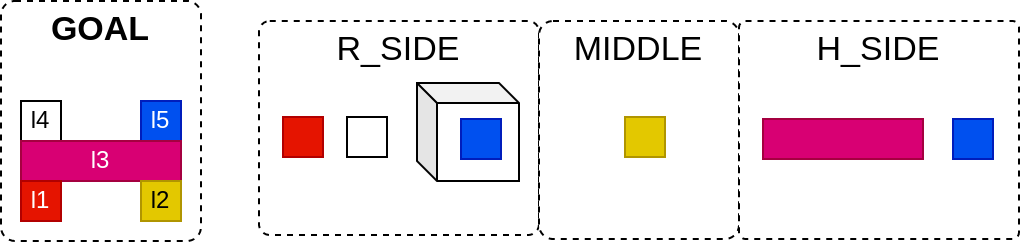
\includegraphics[width=\linewidth]{Chapter4/block_world_domain.png}
    \caption{An instance of the BlocksWorld domain. The ideal plan is strongly influenced by the human desired preferences. For the earliest end of the task, the human prevents using the box. A lazy human will only place the required pink bar from their side. And a human in a hurry will place concurrently the yellow cube to place the pink bar at the earliest and be able to leave.}
    \label{fig:block_world_domain}
\end{figure}


    \subsection{Human behavior and erroneous estimated preferences}

To simulate the human behavior, we consider and define human preferences that produce a human policy in the same manner as for the robot. The produced human policy makes the human always perform the best action regarding their defined preferences. The robot/planner doesn't have access to the human preferences but only to an estimation of them.

In order to evaluate the quality of the executed trace regarding the actual human preferences we compare and rank every possible trace from the search graph, from best to worst. For legibility purposes, we normalize the ranks to obtain a score (H-score) s.t. the trace/plan with the lowest rank has a score of 0.0, while the highest rank corresponds to a score of 1.0. This score represents a quality indicator independent of the instance's size. 
Similarly, we can do the same and acquire the score regarding the robot's estimation of the preferences (R-score). 
Keep in mind that the R-score is an estimation of the actual H-score, and the robot acts in order to maximize its R-score, hoping to maximize as well the H-score.

However, the estimation of the human preferences can be more or less accurate, causing the robot's decisions to differ from what humans would have preferred. Once again, that's why making the robot compliant with human online decisions and actions gives the human more influence over the execution and helps to reach high H-score even when the robot's estimation is incorrect.
Despite the robot trying to maximize its R-score, it's important to note that reaching a low R-score is fine as long as a high H-score is attained.

\begin{figure}
    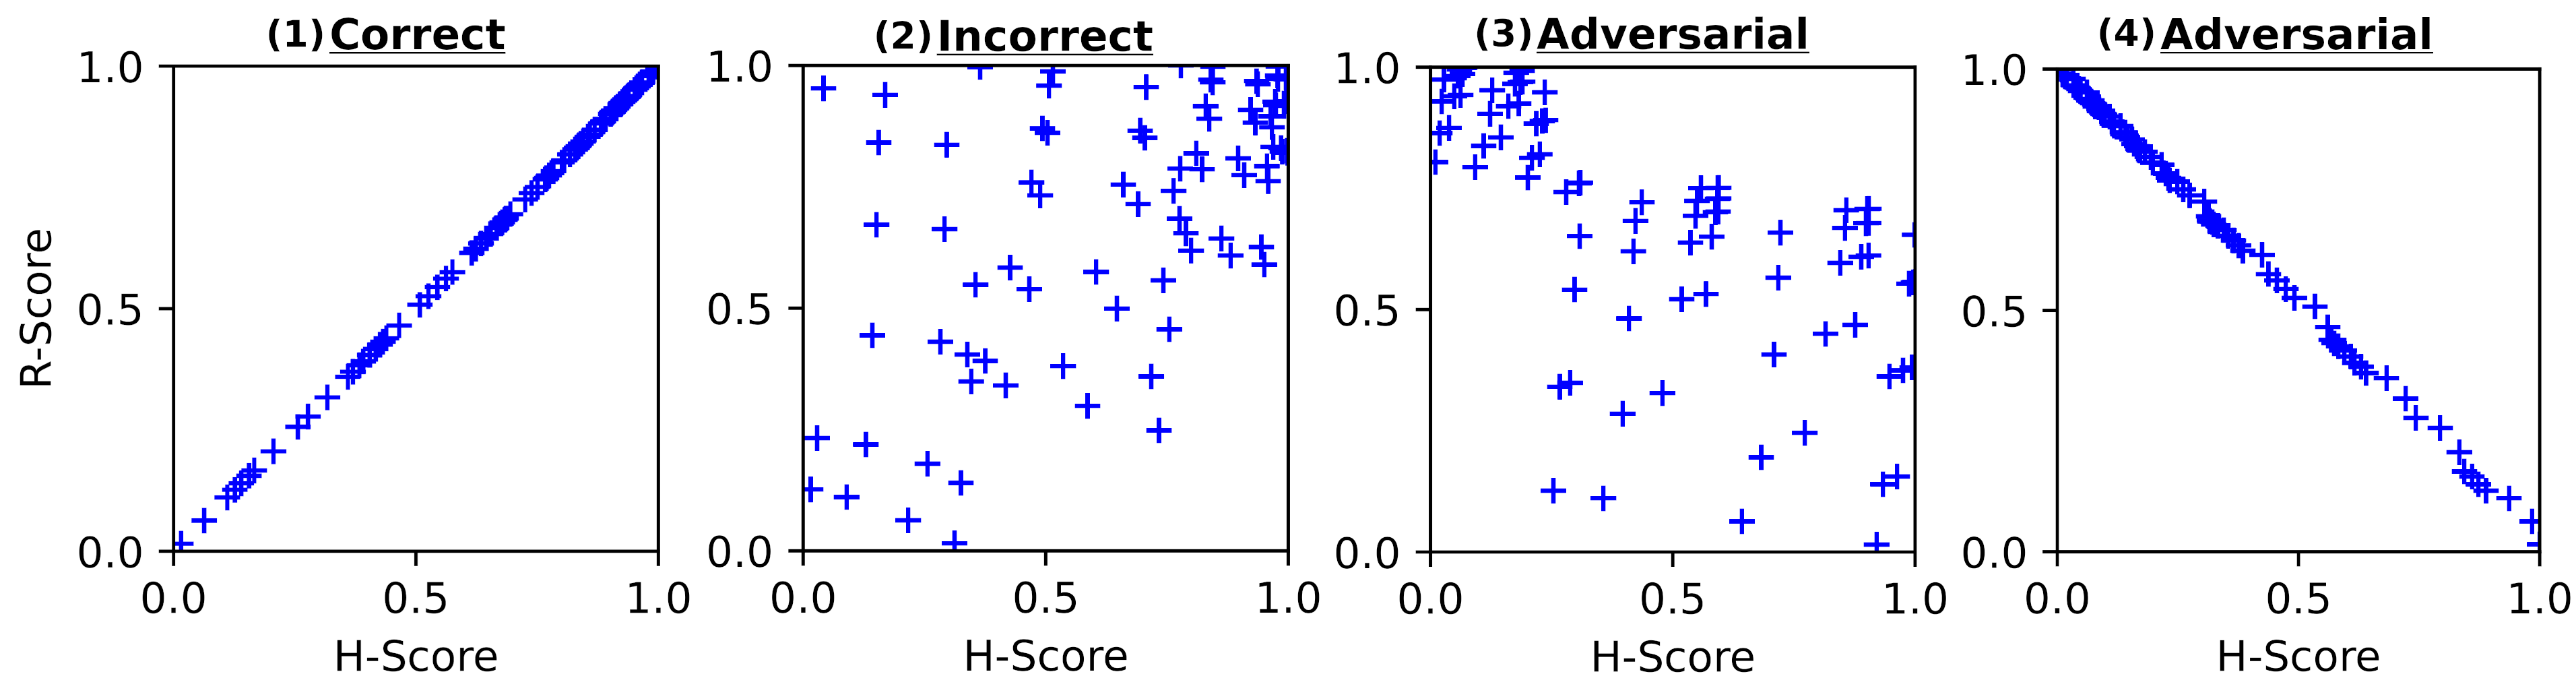
\includegraphics[width=\linewidth]{Chapter4/all_corr.png}
    \caption{
    Correlation between the H-score and R-score according to different robot estimations. Four pairs of human preferences and their estimation are considered. For each pair, all possible traces are plotted as blue crosses according to their H-score and R-score. \textit{(1)} show a correct estimation while the others show incorrect estimations. \textit{(3)} and \textit{(4)} depict \textit{adversarial} estimations.
    }
    \label{fig:corr}
\end{figure}

In practice, a pair of human preferences and their estimation creates a correlation between the possibly obtained H-scores and R-scores when solving the task. Figure~\ref{fig:corr} depicts several possible correlations for a same task and same search graph but different pairs of human preferences and their estimation. On each sub figure are shown all possible traces as blue crosses according to their H-score and R-score. 
Let's consider the first case where the estimation is perfectly accurate (correct). Here, the choices of the robot which are maximizing the R-score will necessarily maximize the H-score. Indeed, when considering the few top possible robot plans (crosses with near $1.0$ R-score), the human preferences are always well satisfied (near $1.0$). 
Let's now consider the second case where the robot estimation is incorrect. Here when considering again the few top possible robot plans a wide range of H-score can be reached (near $1.0$ as well as close to $0.0$). Thus, an incorrect estimation can satisfy the human preferences but not necessarily, and so, can also fail to comply with them.
Eventually, consider the last two cases. Here, the lack of blue crosses in the top-right corners means that the H-score cannot be near $1.0$ while also having a high R-score. As a consequence, when maximizing the R-score the robot will necessarily deteriorate the quality of the plan w.r.t. the H-score. We refer to these cases as \textit{adversarial} estimations since the robot, involuntary, goes against the human will. Such cases occur when the robot estimation is far from the actual preferences and intuitively going against the latter, for instance, the robot trying to minimize the human effort while the human is actually trying to do as much as possible.  

    \subsection{Results}

\begin{figure}
    \centering
    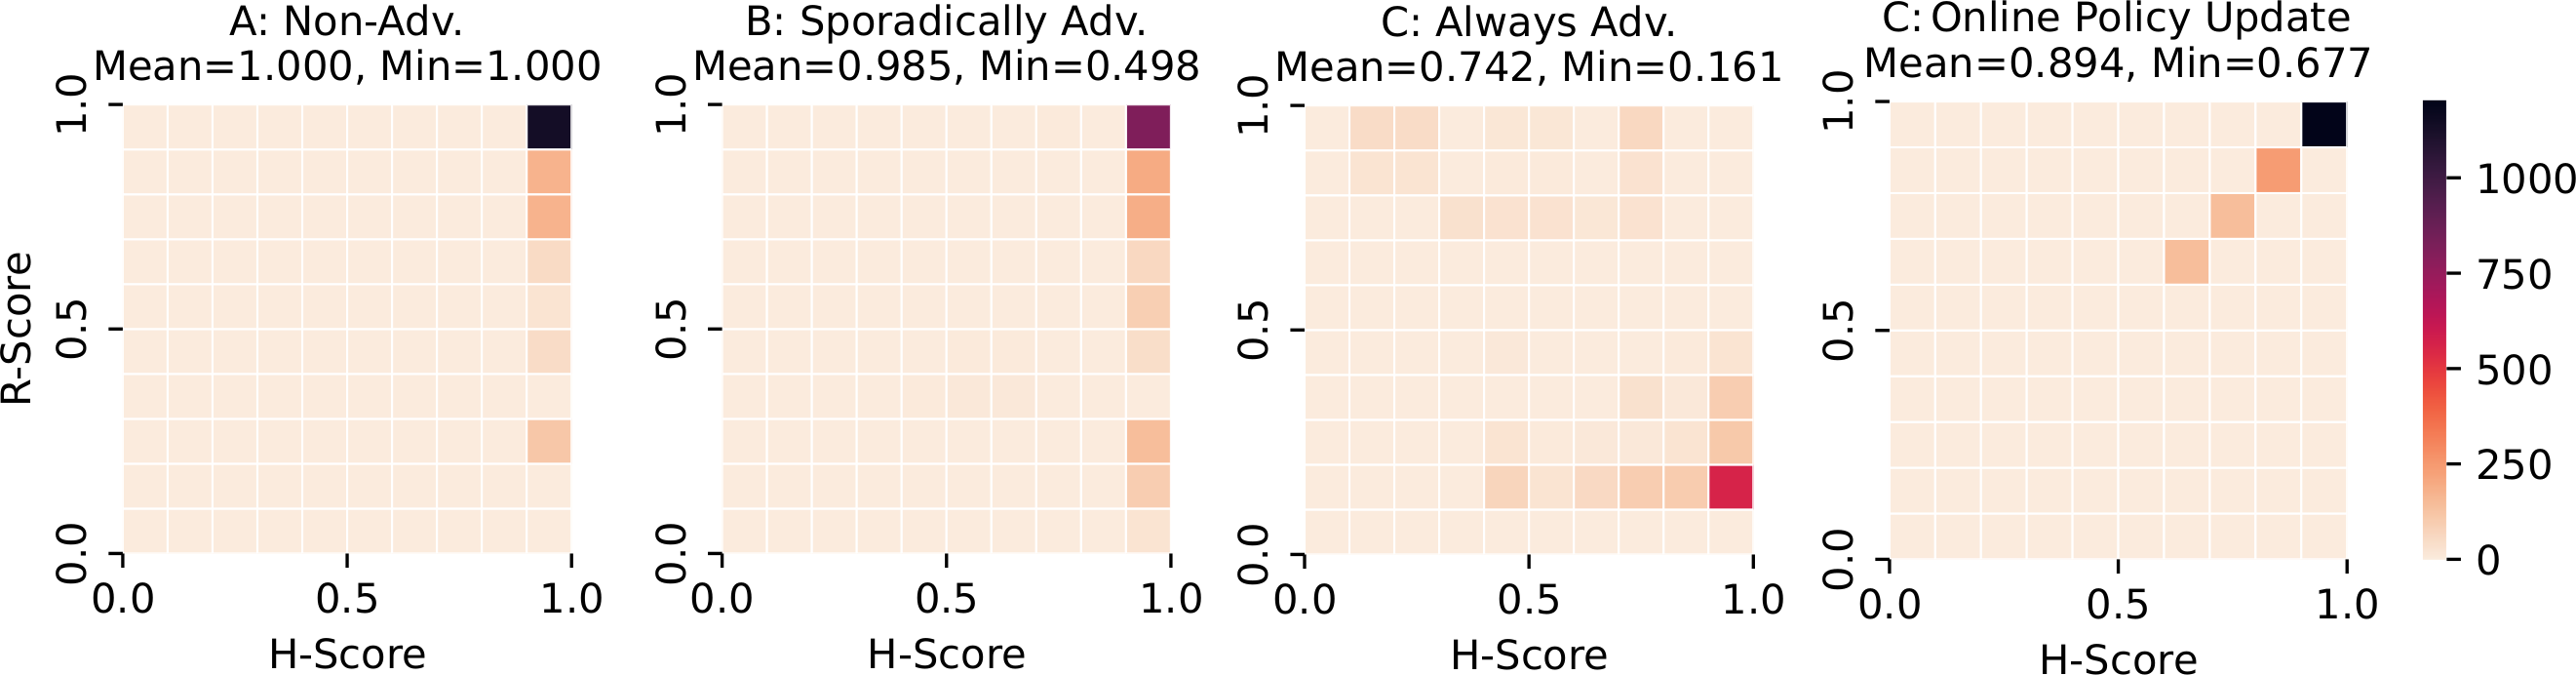
\includegraphics[width=\linewidth]{Chapter4/quant_results.png}
    \caption{
    R-scores and H-scores of the obtained executed plans after simulating the execution of the robot and the human policy generated by considering three problems and three sets of pairs of preferences/estimations. 
    The estimations in each set are (A) Never, (B) Sporadically, and (C) Always adversarial. On the right, it is shown the scores obtained using an enhanced human policy that can correct online the robot's estimation while using the set (C). \textbf{TODO: [show H mean+min and R mean+min ?]}
    }    
    \label{fig:heatmaps}
\end{figure}

For the simulations, we first generated three problems of the BlocksWorld domain with different initial states and shared tasks, and we produced for each their corresponding search graph. 
After, we generated numerous pairs of human preferences and associated robot estimation, all those pairs are categorized in three distinct sets.

In Set~A, the estimations are mostly correct and close to the human preferences (case \textit{(1)} in figure~\ref{fig:corr}). Set~B includes incorrect estimations (case \textit{(2)} in figure~\ref{fig:corr}). And Set~C contains only adversarial estimations (cases \textit{(3)} and \textit{(4)} in figure~\ref{fig:corr}).
Then, for each preference-estimation pair and each problem we generated the associated human and robot policies. Their execution was simulated symbolically using an execution automaton directly shaped upon the presented Model of Execution, and the obtained executed trace were retrieved.
The R-score and H-score of every obtained executed trace are shown as heatmaps for each distinct set of pairs in Figure~\ref{fig:heatmaps}. This will help us to highlight the benefits of using such execution scheme.

In Set~A, the estimation of the robot is close to the real human preferences and is never adversarial. So, the robot policies (maximizing the R-score) should naturally lead to high H-scores, and this is what we observed.
Some plans had an R-score lower than $1.0$ showing that the estimation was not perfect. Yet, the compliance to the human actions and the non-adversarial choices of the robot allow to always satisfy the maximal H-score of $1.0$, and thus, to always satisfy the human preferences. 
With Set~B, the incorrect estimations induced some detrimental robot choices, preventing the human from always reaching a score of $1.0$. This is depicted by the minimal H-score of $0.498$ obtained. Nonetheless, the average H-score of $0.985$ indicates that the human preferences were overall largely met.
Set~C captures the worst possible estimations inducing the robot to always make adversarial choices. This is depicted by the lower average H-score ($0.742$) and the very low minimal H-score obtained ($0.161$). 
Yet, we can notice that the average H-score is still high and that the R-score drops significantly. A low R-score means that the robot wasn't able to follow its policy correctly. Indeed, thanks to our model of execution, the robot comply to the human online decisions and purposely deviate from its ``optimal'' policy to let the human follow their own optimal policy. Eventually, the relatively high H-score obtained shows that the compliance is effective and compensates significantly (of course not totally) for a very poor estimation of human preferences. 

Additionally, we can reasonably complement the human policy, which is so far only based on preferences, with a \textit{rule}. Whenever the robot performs an action that degrades significantly the best reachable H-Score, then the human reacts by correcting online the robot estimation.
The rightmost sub-figure in Figure~\ref{fig:heatmaps} shows the new scores obtained using the Set~C and the complemented human policy. 
We notice that correcting online the estimation avoids very low human scores (minimum of $0.677$), and increases significantly the average H-score as compared with the original Set~C results (from $0.742$ to $0.894$). Hence, making the robot compliant with online preferences is very effective in improving the quality of the joint plan executed.

\textbf{TODO: [Comparison with baseline ??? ... this lack was criticized... A simple baseline with Robot first? Should show that on correct is fine but then H-score is highly degraded... Should be a mirror case of our results However, must replicate results and create more... currently unclear if can replicate.]}

Overall, we can see that the compliant robot behavior regarding both online human actions and preferences benefits the collaboration thanks to the high human scores obtained.

Consider some counter-cases from social robotics (or HA collaborative planning). Assume a robot not giving the initiative to humans always executing the best action it found. 
It is less acceptable and restricting for humans this way, even if the robot computed its best action by taking into account some social rules and estimated preferences. 
Unlike here, humans would appear compliant with the robots. 
In those cases, as it is evident from our simulation results in adversarial setups, the robot strongly impacts the solution H-score. Thus wrong robot choices can significantly degrade the human scores. In some sense, being compliant and adjusting to online preferences can be seen as some social factor that robots should maximize, and our framework helps achieve that.

\section{Performances}


In this section, we discuss the computational performances of our approach and provide some empirical measurements. 

Our approach is based on exploring every decision the human is likely to make and every possible robot concurrent and compliant actions to those decisions. 
This offline search produces a directed acyclic graph (DAG) which captures all possible courses of action. Then, from this graph, we can easily extract online the optimal robot policy to adapt to and to satisfy the human preferences. However, this exhaustive approach does not scale since the more complex and long the task is, the more possible coodinations and courses of actions exist, and the longer it takes to produce the graph. Despite this existing combinatory explosion, I would like to discuss and explain why our approach is still relevant.

Two cases can be identified. The first one is in industrial setup and the other in a household environment. Industrial tasks can be complex, constrainted, and where mistake can have heavy consequences. However, household tasks are usually simpler, shorter, and have fewer constraints and consequences. Due to the nature of industrial tasks, there is usually a known pre-defined protocol or plan to solve the task. The human is also in a working mental state, being more focused and willing to collaborate and accept robot decisions. This means that in such setups, it is more acceptable for the robot to produce a joint plan and negociate with the human to accept and follow it, without anticipating every possible human decisions which significantly reduces the complexity of the planning algorithm.
On the other hand, when considering household tasks, which is more our focus in this work, we want to preserve the human's latitude of choice as much as possible to allow them to change their mind, be distracted, or impose their choice. For this reason it is effective to run an exhaustive search and account for every possibility. 

Overall Human-Robot Collaboration scenarios never requires long plans, especilaly household taks, and are often limited to about 20 actions per agent. For such length, our exhaustive approach performs efficiently. Its takes about $0.40s$ for our approach to produce the DAG for the BlocksWorld task described in chapter~\ref{chap:6}. This graph comprises $700$ nodes and $6$ leaves, corresponding to $6839430$ different possible plans of length $19.77 \pm 1.59$ steps. With millions of plans we explore sufficient possibilities to address correctly such collaboration problem. Moreover, it takes only $0.02s$ to extract the robot's policy from the produced graph. 

\textbf{TODO: Try to add more numbers, about the task of Chapter 4 with box, and about more complex and long tasks}


\section{Discussion and Limitations}


This section discusses a few limitations of the proposed approach and possible future works to overcome them. 

First, in order to explore relevant courses of action, we assume a step-based progression toward the goal. Hence, we assume that the human and the robot must synchronize together after every action. This can work efficiently as long as we assume that all actions have roughly the same durations. However, in practice, this is never exactly the case and one agent must wait for the other at every step. Since the robot tends to be slower, the human might have to often wait for the robot during the collaboration with these assumptions. To be implemented on a real robot, this approach requires an additional execution scheme supervising the plan execution. In specific situations, this scheme could skip one synchronization and synchronize after the next step. Such a scheme could allow the human to perform more actions than the robot before synchronizing and thus promote a smooth and flexible execution.

Speaking of execution, the results presented in this chapter have only been simulated symbolically, without durative actions nor real human decisions. The next two chapters (\ref{chap:5} and \ref{chap:6}) present a user study conducted on an interactive simulator where participants collaborated with a simulated robot executing the produced policy. To do so, we created an execution scheme able to supervise the execution of the robot policy with agent synchronizations. This scheme is directly based on the model of execution presented in fig.~\ref{fig:complete_model_exec}. Thus, it relies on the steps and doesn't provide the flexible execution mentioned just above. 

Additionally, in the proposed model of execution, the robot always gives the initiative to the human. We show that this decision makes the collaboration robust to erroneous human preference estimations, and thus, is beneficial. However, it could be relevant for the robot to sometimes intelligently switch from follower to leader. Indeed, currently, even when there are no possible conflicts between agents' actions, the robot waits for the human to start acting to begin. Such synchronization isn't really necessary, so the robot could start acting directly to solve the task faster. 

Eventually, the plan evaluation is a bit limited. For now, plan selection relies on the estimated human preferences which are a list of metrics to maximize or minimize in the priority order given by the list. This means that there is no balance between the metrics so, depending on the ordering, a plan of length $N$ where the robot is never intrusive and always compliant could be rejected against a plan of length $N-1$ where the robot is intrusive twice and never compliant. 
Yet, in our examples, we tend to explore numerous very similar possible plans. Thus, there are always several possible plans with a same top-priority metric value, e.g. plan length, and the ordering will help select the best plan satisfying at best the other listed metrics.   

\section{Conclusion}

We addressed the complex challenge of concurrent task planning for a shared goal in the context of human-robot collaboration, acknowledging the inherent need for autonomy in humans' choices of `what' and `how' aspects during task execution. 

Based on studies about joint action, we formulate an execution model, and we present a new human-aware task planner designed to accommodate the uncontrollability factor inherent in human agents while employing this execution model leveraging social signals to facilitate the exploration of human-robot joint actions and a smooth execution. 
We also propose a plan evaluation and selection based on estimations of the human inner preferences.
As a result, the planner produces the behavioral policy for a robot that complies with online human decisions and their (online) provided estimated preferences, 
ensuring it solves the task, satisfies at best the estimated human preferences, and allows smooth and sound execution of concurrent joint action.

We provide a detailed account of the novel planning process and joint action model. We demonstrated its effectiveness through symbolically simulated BlocksWorld scenarios and how our model makes the robot robust to erroneous preference estimations.

Additionally, as mentioned in the previous section, we implemented an interactive simulator in which a real human can collaborate with a simulated robot running the generated policies. We used this simulator to conduct a user study to validate our approach with real humans. This simulator and study are described in the next two chapters.  

\newpage
\thispagestyle{empty}
\mbox{}

\ifdefined\included
\else
\setcounter{chapter}{4} %% Numéro du chapitre précédent ;)
\dominitoc
\faketableofcontents
\fi

\chapter{Implementing a Joint Action Execution Scheme in an Interactive Simulator}
\chaptermark{Interactive Simulator}
\label{chap:5}
\minitoc

\chapabstract{
The joint action model we proposed in the previous chapter was abstracted and used to guide our planning approach. This chapter proposes implementing this model as an execution scheme integrated into a dedicated simulator. The latter allows human operators to collaborate with a simulated robot, executing the policies produced by our planning approach. We provide more details about our joint action model and technical details about the developed simulator used to conduct a user study, which will be described in the next chapter.
}

\section{Introduction}

In order to validate the approach presented in the previous chapter (\ref{chap:4}), we would like to be able to perform a task collaboratively with a simulated robot executing the produced policy.
For that, we refined our model of concurrent and compliant joint action execution. In Chapter~\ref{chap:4}, this model was abstracted and used to guide the planning process to explore further relevant courses of action. As another contribution, we implemented the model as an execution scheme capturing subtleties and social cues of a smooth collaboration. Then, we integrated this scheme into a simulator, allowing human operators to collaborate with a simulated robot running policies produced by our planning approach. An overview of the complete system is shown in figure~\ref{fig:architecture}.
Eventually, we used this simulator to conduct a user study, which will be described in the next chapter. 


\begin{figure}[h]
    \center
    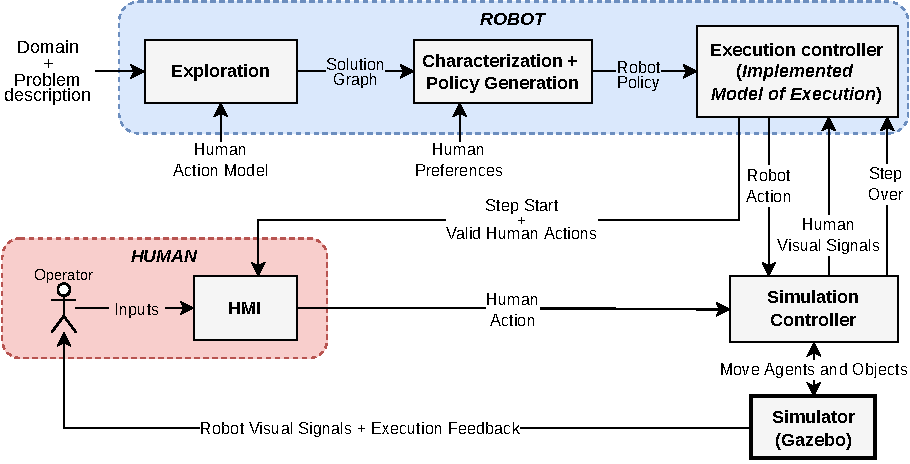
\includegraphics[width=\textwidth]{Chapter5/architecture.pdf}
    \caption{Overview of the Interactive Simulator's Architecture}
    \label{fig:architecture}
\end{figure}

This chapter first presents details about the refined joint action model and highlights the additions compared with the abstracted model presented in Chapter~\ref{chap:4}. Then, technical details about its implementation and the overall simulator are given. After describing the simulated scene, details about the various controllers used to run the simulator are provided. We also explain how a human operator can interact with the simulator and effectively collaborate with the robot. Finally, we describe the data we collect during and after each collaboration. 


\section{Execution Controller - Joint Action Model for Execution}

The model of execution presented in the last chapter was simplified and abstracted to be used to guide the planning algorithms and explore further relevant courses of action. This allows for anticipating possible coordination and compliance with online human decisions. 
However, we need an execution controller to supervise the execution of the produced policy. Here, we propose a refined and implemented model, matching the abstraction previously made, to be able to execute the produced robot policy and supervise its execution by synchronizing with the human through social signals.

The next page depicts the complete model in fig~\ref{fig:complete_model_exec}. In addition to refining the `robot automaton' present in the abstracted version, it also models the human agent's behavior with another automaton that captures the possible decisions the human may make during execution. Additionally, this complete model makes all the social signals exchanged between the agents explicit and shows how they are used for coordination. These differences are discussed in detail below. This execution controller takes as input the solution \acrshort{dag} produced by the approach of Chapter~\ref{chap:4}. Then, the controller progresses from the initial state to a goal state in the solution graph. The controller handles the state transitions, step by step, by sending and synchronizing on social cues. Thanks to this controller and the associated simulator, we now have a durative task execution that effectively affects a simulated environment.

\begin{sidewaysfigure}
    \centering
    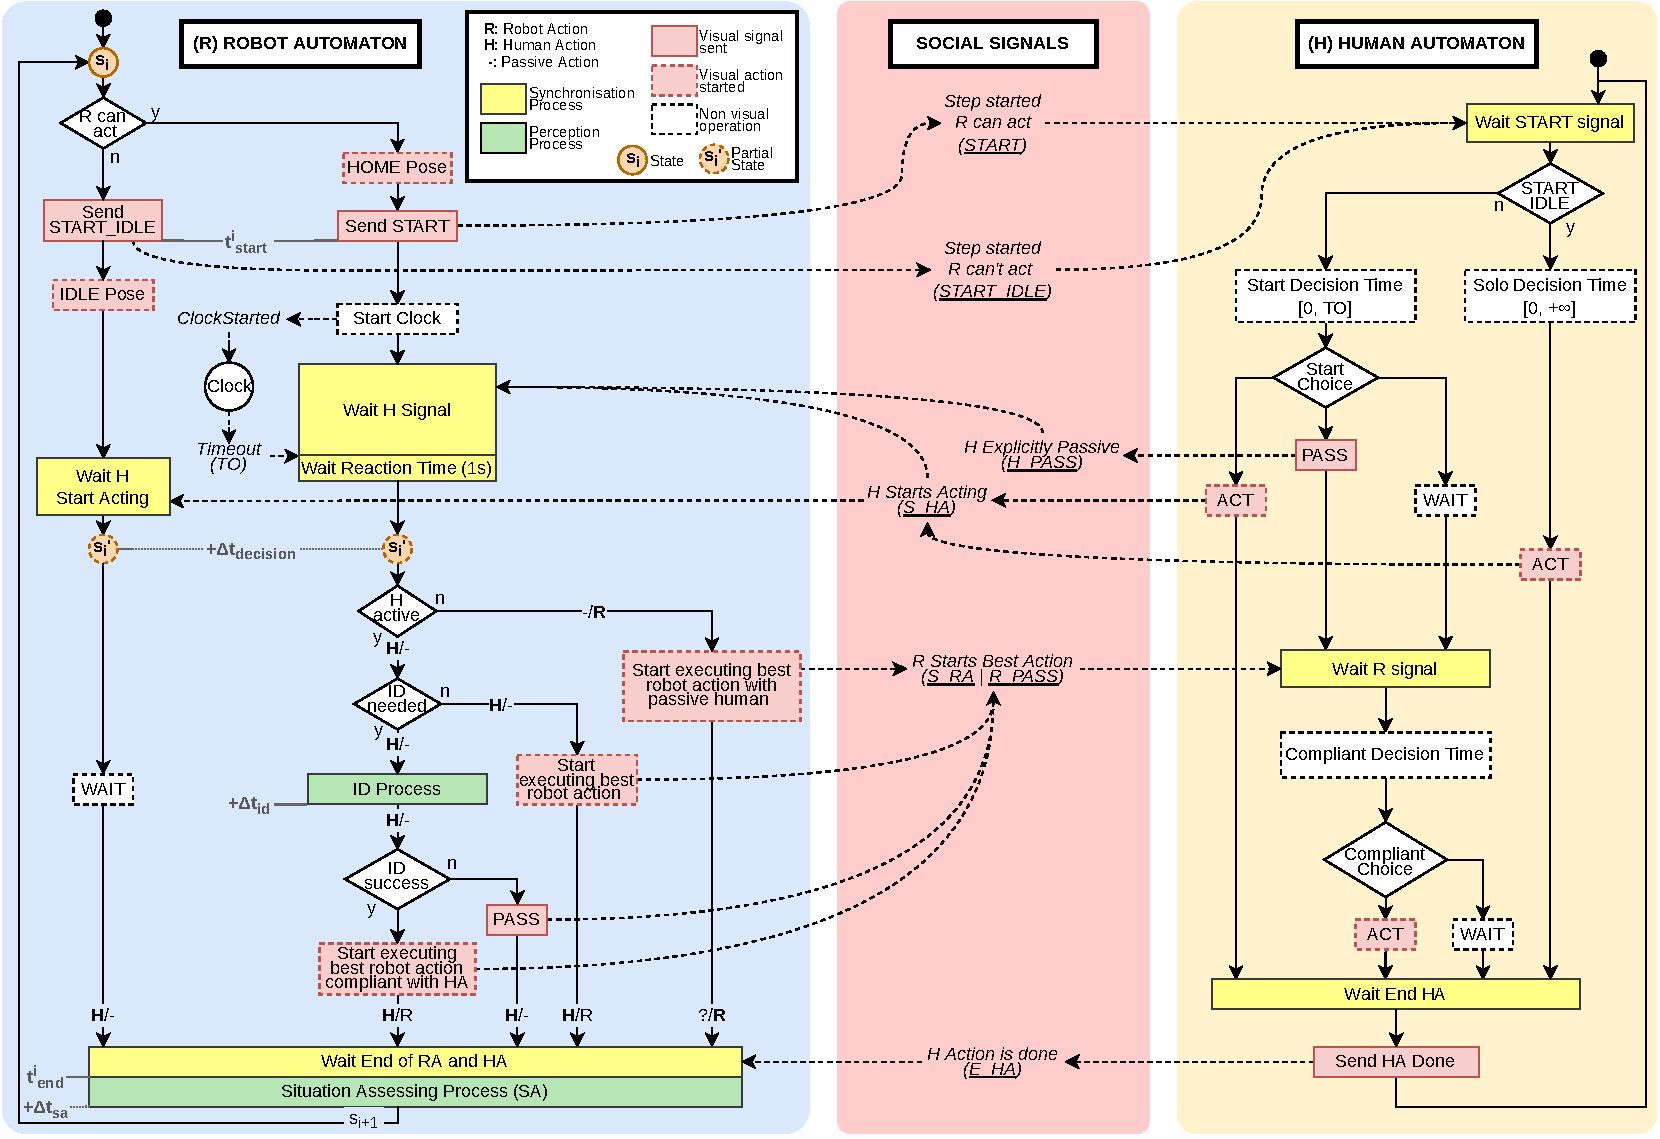
\includegraphics[width=1.0\linewidth]{Chapter5/complete_automaton.pdf}
    \caption{Complete Model of Concurrent and Compliant Joint Action used as an execution scheme. This version details the robot automaton and the assumed human automaton as well as the visual signals exchanges between the agents to synchronize themselves.}
    \label{fig:complete_model_exec}
\end{sidewaysfigure}


In the execution controller, the robot automaton is refined and more detailed. 
First, we show the social cues sent by the robot, which are the following: \textit{START} corresponds to the visual and audible signal indicating to the human that the step begins; \textit{S\_RA} corresponds to the start of a robot action; \textit{R\_PASS} corresponds to the robot being explicitly passive. The other signals, including the human ones, will be described below.
Also, we modeled the case where the robot cannot act in the current step. This can be determined easily given the search graph and the current state $s_i$ and by checking if there is at least one non-passive robot action in the following arcs. This checking process is represented in the figure by the diamond shape with the label ``R can act'', and the respective positive and negative answers ``yes'' (y) and ``no'' (n). When the robot cannot act, it sends a specific signal to inform the human that the step has started and cannot act (START\_IDLE), then goes in the \textit{IDLE} pose. This is a visually passive posture where the robot looks at the human with its arm retracted, indicating that it cannot act. Only a human action can progress to the next state. Thus, the robot waits for this action to start and eventually finish. Then, the Situation Assessment process identifies the executed action, and thus, the new state $s_{i+1}$ to continue. Depending on the possible actions, the robot can stay in this \textit{IDLE} pose for several steps. Once the robot can act again, the ``yes'' branch of the automaton is followed, and the robot returns to the \textit{HOME} pose. In this posture, the robot's arm is deployed, showing that the robot is ready to grab objects on the table.

Additionally, the process of waiting for a human signal at the beginning of each step is more detailed. This process is interrupted by one of the three following signals: \textit{H\_PASS} is an explicit signal (hand gesture, verbal communication) sent by the human to share its desire to be passive; \textit{S\_HA} is the start of human actions, and is detected by tracking human's motion; \textit{TO} is the internal timeout signal sent by a clock $4s$ after the start of the waiting process. 
However, the perception layer on a real robot would induce a delay in this synchronization process. 
An additional waiting time of $1s$ is added to compensate for the robot's reaction time, allowing the human to send signals just before the timeout. Without it, the human could start moving just before the timeout, but the robot would interpret this information too late and consider them as passive.
Note that the robot only waits for a human signal if the human can act in the current step. This check is done similarly to the first diamond process. However, it is not shown in the figure for legibility reasons. Hence, it means that in situations where only the robot can act, it will not wait and will directly start acting.

% Remember that this process only identifies an explicit signal like a predefined hand gesture or the start of a human motion. In the case of human motion, we do not yet identify which action the human is starting. This is achieved by the dedicated Identification (ID) process, which is longer and here about $0.6s$. Thus, we believe that the chosen duration of $0.3s$ is relevant for detecting the initial human signals. 

The last visual difference with the abstracted model on the robot's side is the case where the human decides to be passive. In this branch, the human decision is pictured as a question mark. This is because we first identified the human as passive, and thus, the robot performs the best corresponding action provided by the policy. However, while the robot is acting, the human is free to start performing any action that does not conflict with the already-started robot's action. These possible decisions are modeled in the human automaton described after but are identified by the robot only during the Situation Assessment process. 

On the other hand, a human automaton now explicitly models how humans should behave to coordinate with robots and collaborate successfully. This automaton starts by always waiting for the beginning of the current step, indicated by the robot with the signals \textit{START} or \textit{START\_IDLE}. The simplest but less common case is when the robot cannot act during the step (after receiving \textit{START\_IDLE}). This case is depicted in the rightmost branch. Since the robot cannot act, only the human can make progress in the task by acting. Thus, the human is free to take as much time as desired, represented by the decision time in the range $[0; +\infty]$. After the start of the human action, both human and robot automatons wait for the end of the human action, and then they proceed.
Let us discuss now the most common case where the robot can act. This time, the human must decide before the defined robot timeout (TO), otherwise they will be considered passive. The human can decide either to start acting (ACT), to indicate their passivity (PASS), or do nothing corresponding to being passive without informing the robot (WAIT). If the human decides to be passive (PASS or WAIT cases), they can either remain passive until the next step or decide to perform an action not conflicting with the robot one. This is represented by the last human diamond shape labeled ``Compliant choice'' made after a duration referred to as ``compliant decision time''.


\section{Gazebo Simulated Scene}

This interactive simulator is based on the Gazebo Simulator. It is an open-source 3D simulator able to simulate articulated robots in a dynamic and complex environment.
This section describes all aspects directly linked to this existing 3D simulator on which our framework has been developed.

The overall scene is depicted in the figure~\ref{fig:simu_view}. The stacking goal is displayed in the top left corner, and a text prompt is shown in the top right corner so that the robot can communicate with the human.

\begin{figure}[h]
    \centering
    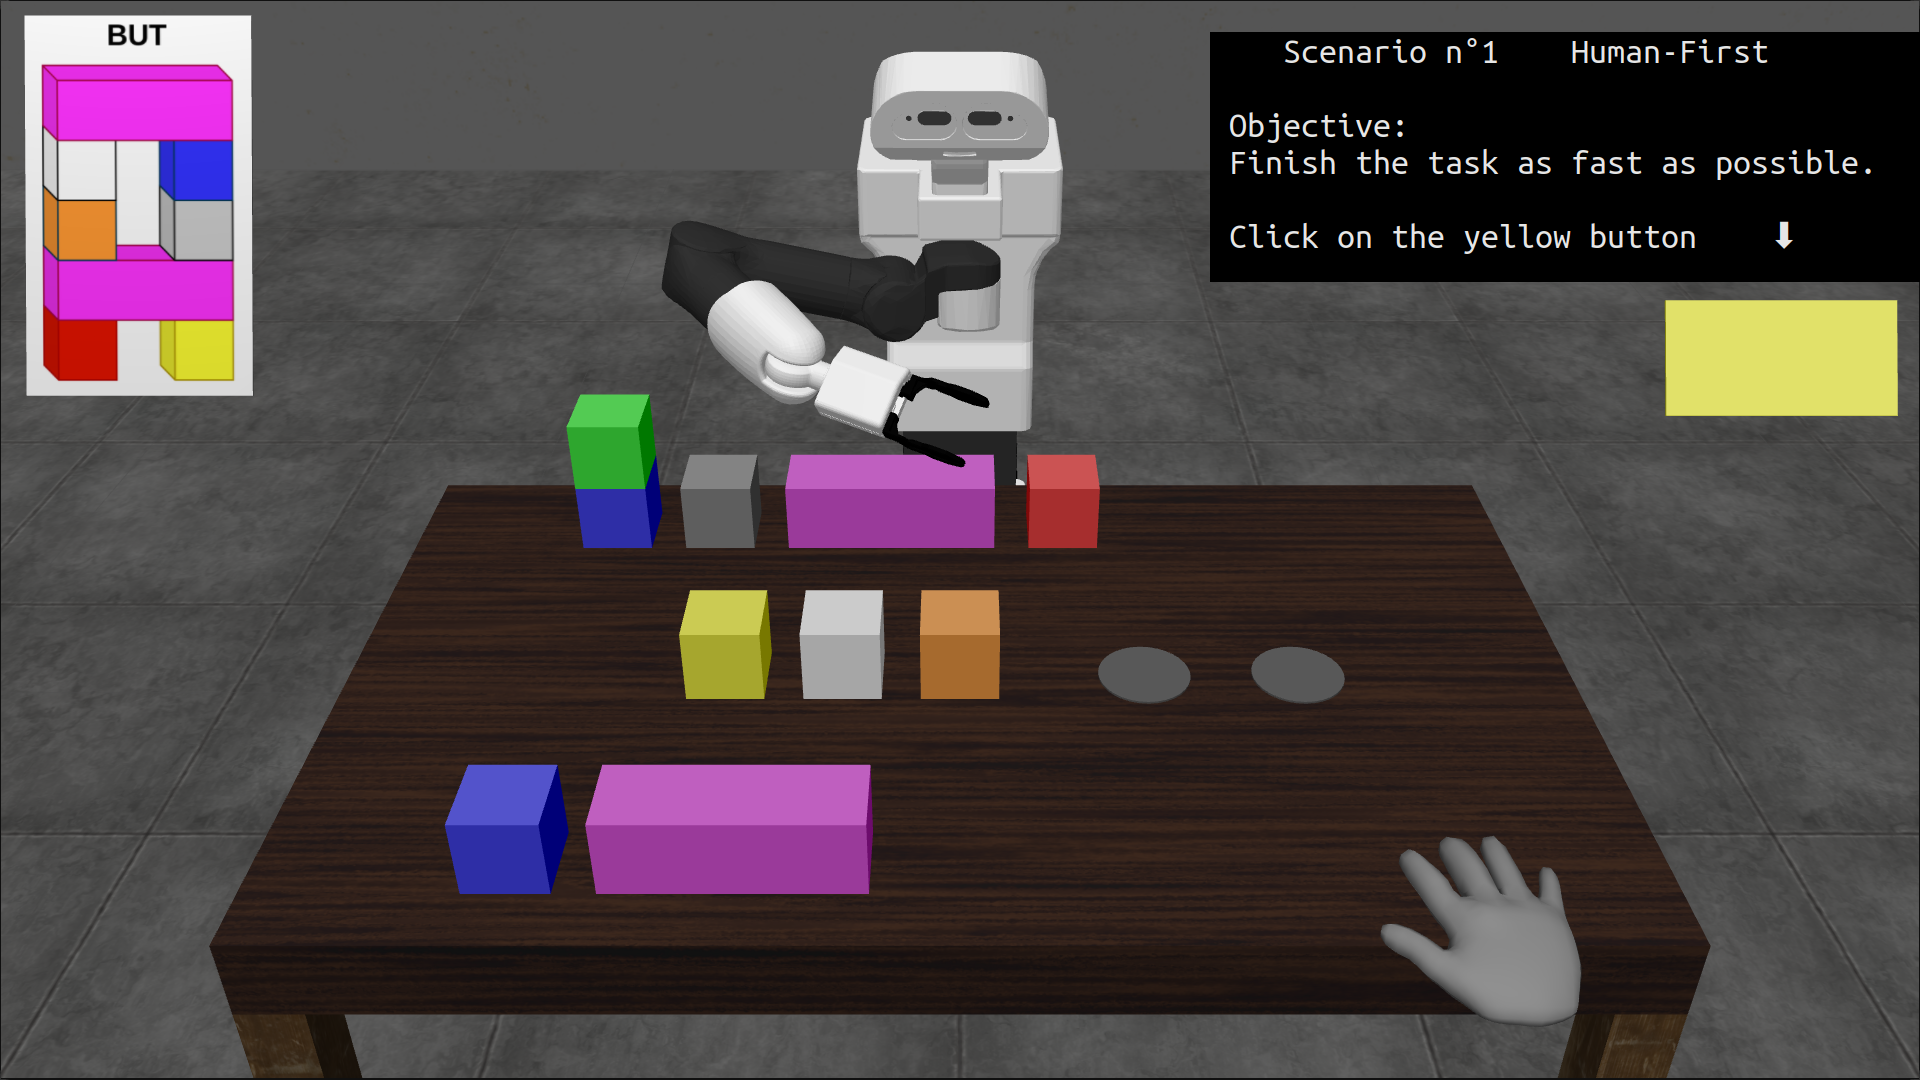
\includegraphics[width=\textwidth]{Chapter5/simu_screenshot.png}
    \caption{Participant view of the interactive simulator. It depicts the colored cubes on the table's left, the stacking area on the table's right (the two darker spots), the goal pattern on the top left, the collaborative robot in front, the text prompt on the top right, and the human hand at the bottom right.}
    \label{fig:simu_view}
\end{figure}

The static scene consists of a large room, with a ground and four walls, and a table placed in the center with two marks on its right side. The marks represent the locations where the cubes must be stacked. The agents are represented as follows. First, the human is represented only with a floating hand as the camera simulates a first-person point-of-view. Then we used a Tiago robot from PAL Robotics because it has an arm to manipulate its environment, a head to send gaze information and signals, and because many related resources are available for it (3D models, controllers, tutorials). The human and the robot are facing each other, each from one opposite side of the table. Finally, colored cubes were disposed of on the table in three distinct zones. Cubes are either close to one agent's side or in the middle of the table. This disposition influences the reachability of the agents as one agent can only reach cubes from their side (just in front of them) or the middle, but never from the other agent's side. This scene corresponds to one specific collaborative task, but another setup could be easily implemented. 

The Gazebo simulator can be integrated with the \acrfull{ros}, which is a set of software libraries and tools that help build robot applications. The main pros of \acrshort{ros} are its ability to run several sub-programs in parallel and allow them to communicate with each other. Hence, the other components of the interactive simulator have been developed with \acrshort{ros}.


\section{Controllers}

Four distinct controllers have been developed to control the simulated agents and the overall simulation execution. Each controller is described below. 

\subsection{Robot Arm Motion}

First, there is one controller that moves the robot's arm. This controller is called with either a 3D position to reach (pose target) or a predefined configuration (named target). In both cases, when called, this controller uses the MoveIt framework. MoveIt creates links between several libraries in order to have access to a unified interface for Motion Planning algorithms, Inverse Kinematics, Control, or Collision Checking. This way, our controller can ``simply'' request MoveIt to find a trajectory to a given position and then make the robot follow this trajectory while taking into account the geometry of the robot arm.

In fact, this controller is slightly more sophisticated. Indeed, in our collaborative context, we prefer the robot to be reactive rather than to have optimal motions. This is why, through the MoveIt interface, we use two different motion planners. The first one is $RRT^*$, which is an optimal planner that stops only when the optimal motion plan has been found. It is desirable to have the robot exhibit consistent and efficient motions. However, this process sometimes takes too much time (4-5s), which breaks the rhythm of the interaction. As a consequence, a short timeout (0.6s) has been set for this optimal motion planner. If the optimal plan is not found within the defined timeout, we use the second motion planner. 
The second planner is $SBL$, which is not an optimal planner. That is, the planner stops when a solution is found, but there is no guarantee of optionality. The major pro of this planner is its speed.
Overall, for every robot arm motion, we first try to find an optimal motion within a short amount of time. If the optimal motion is not found, we quickly find a suboptimal solution to prevent the robot from being passive for too long.

Additionally, to reduce motion planning time, a few simplifications have been done. 
First, collisions are only considered with the table and the robot's body. Hence, the robot arm sometimes goes through the other cubes.
Also, the pick and place orientation are ignored. When picking a cube, the robot gripper just reaches the cube's center from any angle, and then the cube is attached to the gripper. When placing a cube, the robot moves its arm to the target position, and the cube is detached from the gripper. Eventually, the cube's orientation and position are overwritten to match the target location. This way, the robot always performs perfect place action, improving both the reactivity of the robot and its robustness, but the robot's motions are less realistic.

\subsection{Robot Head Motion}

The robot head is controlled to look at various elements during the interaction to exhibit a more intuitive and collaborative behavior. 
Indeed, when waiting for the human, the robot looks at the camera. As soon as the human hand moves to either perform an action or indicate its passivity, the robot starts following the hand to show it is observing the human motions and estimating their intentions.
Then, the robot looks at a cube to indicate its intention to pick it since this is faster than the arm motion. 
Also, the robot looks at the target position when placing a cube to indicate its intention to place the cube there.

A dedicated controller has been developed to perform those head motions based on an existing controller provided in the Tiago robot modules. The existing controller could only change the robot's gaze through a visual and clickable window, allowing an operator to manually click on the scene to change the robot's gaze. This controller has been modified to allow additional features, such as directly requesting to look at a 3D point or an object. Moreover, we can now ask to follow an object. That's how we are able to exhibit the head behavior described just above.  

\subsection{Human Hand Motion}

Moving the human hand requires a dedicated controller but is much simpler than the robot arm motion one. Here, the hand must either move to a position or perform a PASS signal. The PASS signal is a hand gesture indicating to the robot that the human desires to be passive for the current step. This motion is performed by simply rotating the hand back and forth at a constant speed. The PASS motion has a duration of $0.7s$. 
On the other hand, we do not use a real motion planner to move the hand to a target position. We simply compute a straight line between the current hand pose and the target pose. Then, we update the hand position at $50Hz$ to move at a constant speed set to $0.25 m/s$. The planning time is thus negligible compared to the robot motion planning times.

\subsection{Simulation}

Last but not least, I developed a fourth controller called the \textit{simulation controller}. Its main jobs are to decompose high-level actions into low-level commands for the simulator, to keep track of the step-based synchronization used in our joint action model, and to generate the visual social signals used in our model to coordinate the agents. 

\subsubsection{Action Decomposition}

First, we describe how we translate the high-level actions from the plan produced by our task planner to low-level motions that can be executed by the controllers listed above. Some parts of this controller are domain-specific, but a major part is generic for manipulation tasks. This controller received high-level agent actions to execute, such as ``Robot pick(b1)'' for the robot picking the cube b1. The first step is to decompose this action into low-level generic actions, which are themselves made of low-level motions. This controller also keeps track of a few low-level facts to check low-level preconditions, such as what each agent is holding or which object is still on the table. Hence, the controller throws an error when an agent tries to pick a cube while already holding one.

Let's first comment on the low-level generic actions available. This controller is given a list of the object names (cubes) and the names of some predefined locations in the scene (placing locations in the stack). Except for the last five, the following actions are not agent-specific and can be performed by any agent. This is defined by a parameter given when calling the action. The following low-level actions are available:

\begin{itemize}
    \itemsep0em
    \item \textbf{move\_pose\_target:}          moves either the hand/robot arm to a given position.
    \item \textbf{move\_location\_target:}      moves either the hand/robot arm to the position of a given location.
    \item \textbf{move\_obj\_target:}           moves the hand/robot arm to the position of a given object.
    \item \textbf{move\_home:}                  puts the agent in its ``home'' (default) configuration. 
    \item \textbf{move\_named\_target:}         moves the robot arm to the given configuration.
    \item \textbf{grab\_obj:}                   attaches the given object to the hand/robot gripper. 
    \item \textbf{drop\_obj:}                   detaches the given object to the hand/robot gripper.
    \item \textbf{set\_obj\_rpy:}               sets the orientation of a given object.
    \item \textbf{set\_obj\_pose:}              sets the position of a given object.
    \item \textbf{delta\_move\_obj:}            sets the position of a given relative to its current position.
    \item \textbf{human\_hand\_gesture:}        makes a hand gesture to indicate passivity.
    \item \textbf{robot\_head\_look\_pose:}     makes the robot look at a given position.
    \item \textbf{robot\_head\_look\_human:}    makes the robot look at the human (camera).
    \item \textbf{robot\_head\_follow\_obj:}    makes the robot follow a given object.
    \item \textbf{robot\_head\_follow\_hand:}   makes the robot follow the human hand.
\end{itemize}

Then, the high-level actions from the plan produced are the following with their respective simplified low-level decomposition:

\begin{itemize}
    \item \textbf{PickCube:}            Starts by retrieving the cube's current position by sending a request to the Gazebo simulator. If it is the robot, call robot\_head\_look\_obj to look at the cube. Then, call move\_pose\_target with the retrieved cube position. Once over, grab the cube with grab\_obj. After, move\_home is called to retract the robot arm or bring the hand to its initial position. Finally, if it is the robot, it looks to the human with robot\_head\_look\_human.
    
    \item \textbf{PlaceCube:}           Starts by retrieving the position of the target location to stack the cube. If it is the robot, call robot\_head\_look\_pose with this position. Then, we move either the arm or the hand to that position with move\_pose\_target before dropping the cube in the stack with drop\_obj and adjusting its position. After, we go back to the home configuration with move\_home. And for the robot, we look at the human with robot\_head\_look\_human. 
    
    \item \textbf{BePassive:}           The human waves their hand to explicitly be passive. Thus, human\_hand\_gesture is called. The robot does not move and only displays some texts saying the robot wants to be passive. More details about the text prompts will be provided later.
    
    \item \textbf{DropCubeTable:}       When an agent cannot stack a cube they are holding, they can place it back on the table. First, the drop position is defined. It corresponds to the initial position of the cube being held, except for the green one, which is initially on top of another cube and has a dedicated drop position. The robot looks at the drop position with robot\_head\_follow\_pose. The hand or the robot arm is moved to the position with move\_pose\_target. The cube is dropped with drop\_obj, and its position is adjusted. Then, the agent is put in its home configuration with move\_home, and the robot looks at the human with robot\_head\_look\_human.  
\end{itemize}

\subsubsection{Manage Steps Synchronizations}

The simulator controller is also in charge of indicating when a step is over. Since we do not consider steps where both agents are passive, a step begins when an agent starts an action. A step is over when both agent actions are done. These rules cover many situations, such as if the human initially wants to be passive and wave their hand. As a result, the robot starts performing an action, which starts the next step. Currently, the step would be over as soon as the robot's action is over since the human is passive. However, if the human decides to start performing an action concurrently, then the step will be over when both the robot's and human's actions are over. This may imply that if the human starts acting right before the end of the robot's action, then the robot will just wait for the end of the human action, and thus, the end of the step before the next step begins.  

\subsubsection{Send Visual Signals}

The model of execution synchronizes the agents based on explicit visual signals such as the start of a step, the start of an action, the end of an action, or a hand gesture (PASS). Those signals are modeled explicitly inside the system and managed by the simulator controller.

Indeed, when starting an action, the associated visual signal is sent only when the agent starts to move. Hence, we track the arm and hand motions to know when the action is visible to the other agent. Then, when an action is over, the associated visual signal is sent directly. It is worth mentioning that humans will naturally have a reaction time when seeing the robot's visual signals (start/end of action, step start). However, the robot natively does not have any reaction time to such symbolic visual signals. Thus, to simulate the delay introduced by an actual perception module (here perfectly simulated), the human visual signals are delayed to the robot by a reaction time set to 0.3 seconds. This is still quite fast, but at least the robot does not interpret human motions instantly.   




\section{Human-Machine Interface (HMI)}

The human operator, or participant, can interact with the simulation by performing any feasible action during the process. However, humans must synchronize with robots by following the execution model. For this purpose, every step starts with a robot sound/beep. Additionally, a dedicated process receives internally the list of the feasible human actions for the current step. This list is sent by the robot execution scheme and is extracted from the solution \acrshort{dag}. However, the participants do not see or know of feasible actions.

\begin{figure}[h]
    \centering
    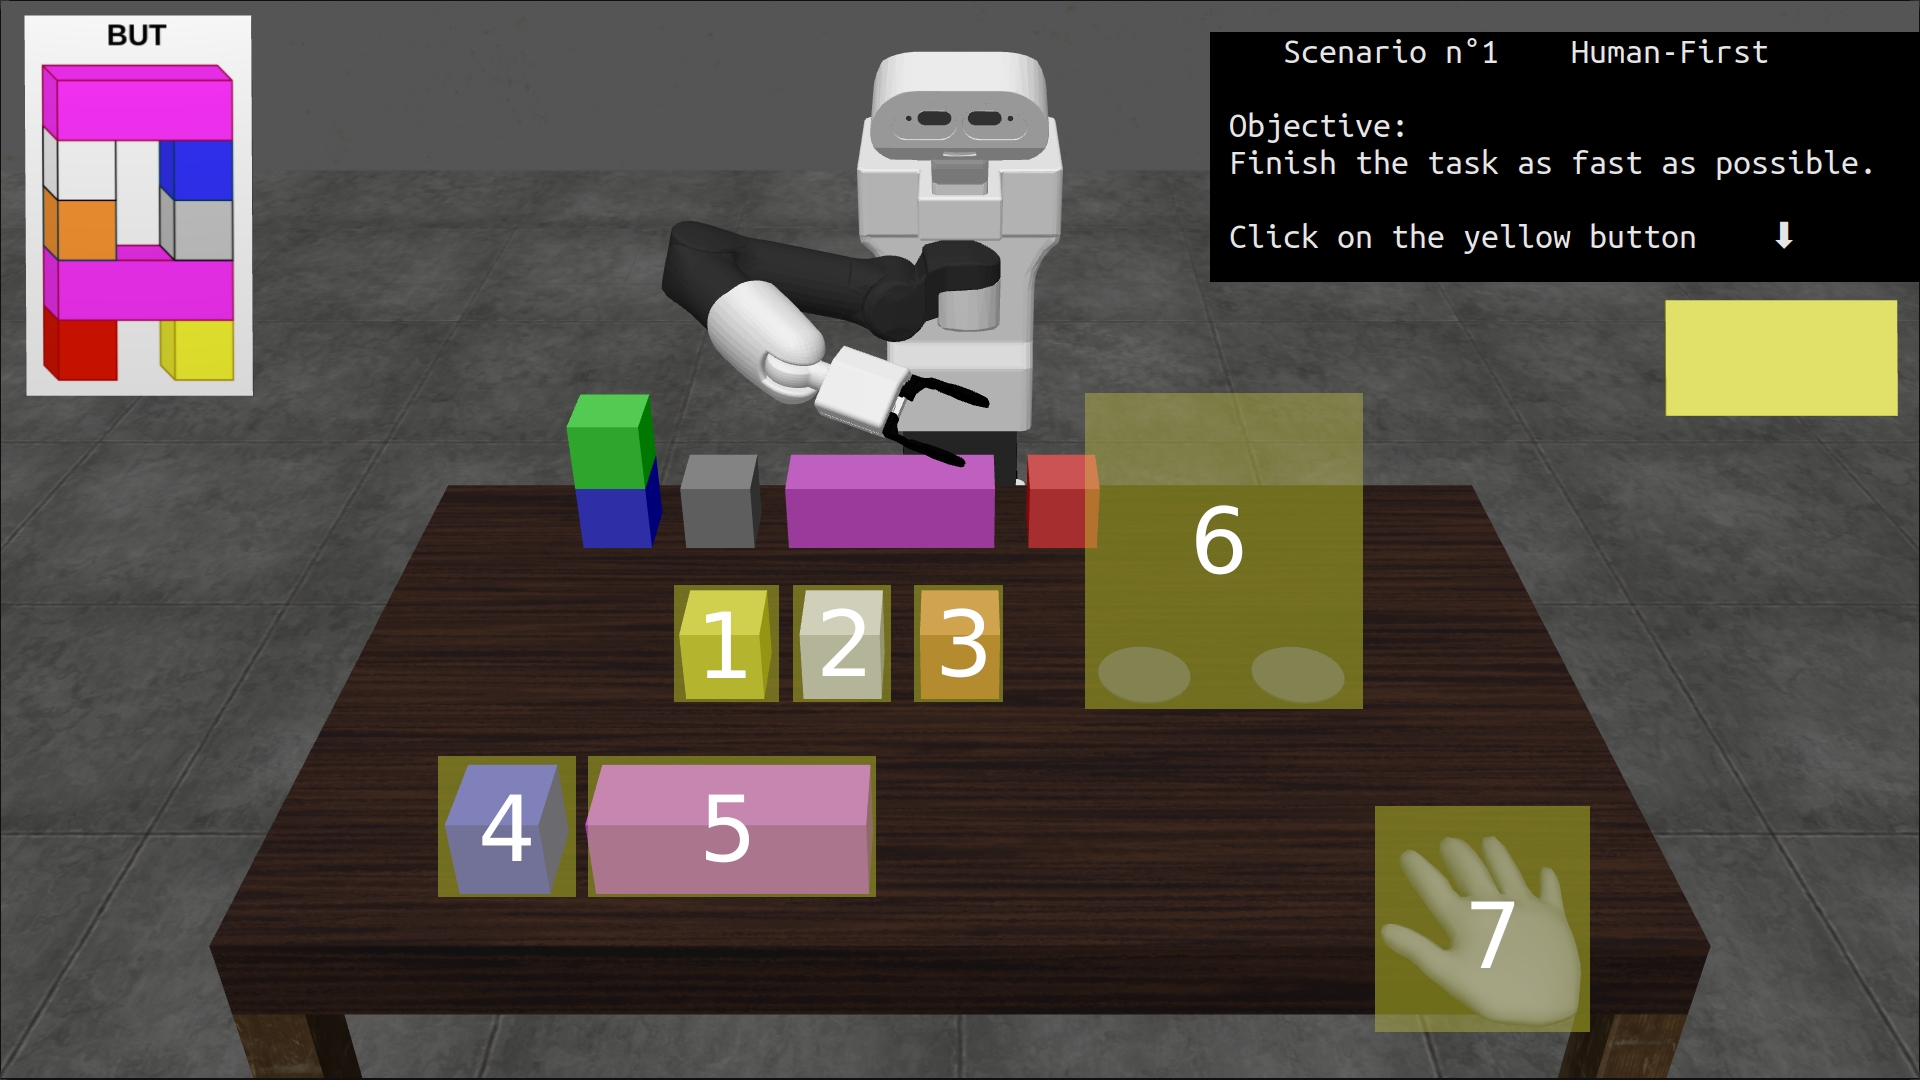
\includegraphics[width=\textwidth]{Chapter5/simu_screenshot_HMI.png}
    \caption{Hidden clickable areas triggering human actions, if feasible. Areas from 1 to 5 trigger picking the respective cube if it is on the table and the human is not holding one already. Area 6 corresponds to placing a held cube in the stack. Area 7 makes a hand gesture indicating the human desire to be passive to the robot.}
    \label{fig:hmi}
\end{figure}

Each possible human action is associated with a rectangular clickable area on the screen. When the human clicks in an area associated with a currently feasible action, the process requests the simulation controller to perform the corresponding human action. Areas 1 to 5 request to pick the corresponding cube if it is on the table and the human is not holding one already. Area 6 corresponds to placing a cube being held into the stack. Since cubes only have one possible stacking place at a time for this task, we consider a large area to trigger placing actions. The controllers determine the exact location to place the cubes. Finally, area 7 makes a hand gesture indicating the human desire to be passive to the robot. It corresponds to sending the \textit{H\_PASS} signal shown in figure~\ref{fig:complete_model_exec}.

\section{Execution Data: Logs, Metrics, and Timeline}

There is also a dedicated process to record the different events and signals during one execution. All other components can send events to log to this process to save them for later post-processing. A log event is defined with a name and a time stamp. Additionally, visual signals are also captured by this logging process and saved both as a signal and as a corresponding event. Logged events mostly help trace the robot's internal states and processes during the execution. The human ones mainly serve to identify when the human is acting or not since we do not have access to the internal reasoning process of the human participant. 

\subsection{Extraction of Agents' Activities}

All logs are saved after each execution and can be loaded later for post-processing. The post-processing involves three steps. First, the agent activities are extracted from the event list. The human and the robot have different possible activities, but since we do not have access to internal human reasoning, there are more robot activities than human ones. The extracted activities are shown in the following table~\ref{tab:agent_activities}. The activities' orders try to match what can happen during the execution, but not all activities are present at every step. Indeed, on the robot side, the ID process is not always necessary and thus not always executed, and the robot either performs an action or is passive for diverse reasons. But the robot always ends up waiting for the end of the step, performing the \acrshort{sa} process and getting ready for the next step. On the human side, if the human performs an action or makes a hand gesture, there will be a measurable decision time. If the human remains passive without signaling the robot, then the only activity is passive without signaling. The ``waiting next step to start'' activity is only added if the human is active. Otherwise, being passive for a step is implicitly equivalent to waiting for the next step.  

\begin{table}[]
    \begin{tabular}{|l|l|}
    \hline
    \multicolumn{1}{|c|}{\textbf{Robot Activities}}                                           & \multicolumn{1}{c|}{\textbf{Human Activities}}                                                       \\ \hline
    Waiting for human decision                                                                & Decision Time                                                                                        \\ \hline
    Identification Process (ID process)                                                       & \multirow{3}{*}{Human Action}                                                                        \\ \cline{1-1}
    Planning arm motion                                                                       &                                                                                                      \\ \cline{1-1}
    Robot Action                                                                              &                                                                                                      \\ \hline
    \begin{tabular}[c]{@{}l@{}}Waiting for human action when\\ itself cannot act\end{tabular} & \begin{tabular}[c]{@{}l@{}}Being passive with signaling \\ (after PASS hand gesture)\end{tabular}    \\ \hline
    Being passive                                                                             & \begin{tabular}[c]{@{}l@{}}Being passive without signaling\\ (after TimeOut is reached)\end{tabular} \\ \hline
    Waiting for the end of the step                                                           & \multirow{3}{*}{Waiting for the next step to start}                                                  \\ \cline{1-1}
    Situation Assessment Process (SA process)                                                 &                                                                                                      \\ \cline{1-1}
    Getting ready for the next step (GRNS)                                                    &                                                                                                      \\ \hline
    \end{tabular}
    \caption{Agent activities extracted from logs. The activities' orders and relative positions try to match the execution, but not all activities are present at every step.  }
    \label{tab:agent_activities}
    \end{table}

\subsection{Metrics Computation}

When loading the execution logs, we extract a set of metrics from the events and extracted activities. Currently, 27 metrics are extracted, but the following table \ref{tab:metrics} only shows 11 because several sub-metrics are hidden. Indeed, for four of the listed metrics, we compute the sum, average, standard deviation, min, and max values of the corresponding metric.

% {\small
% \begin{enumerate}
%     \itemsep0em
%     \item \textbf{Task completion time:}                 Time for the stack to be completed.
%     \item \textbf{Number of steps:}                      Number of steps executed.
%     \item \textbf{Number of human optimal actions:}      Number of human action being optimal regarding a given objective.
%     \item \textbf{Ratio of human optimal actions:}       Number of human optimal actions divided by the number of steps.
%     \item \textbf{Decision time:}                        Time for the human to make a visible decision in a step. Five different metrics are extracted regarding all steps of the scenario: total/sum, average, standard deviation, min and max.
%     \item \textbf{Waiting Next Step:}                    Time during which the human waits for the next step to start. Again, are extracted over all the steps: total, average, standard deviation, min and max values.
%     \item \textbf{Number of human action:}               Number of human actions executed in the scenario.
%     \item \textbf{Human action duration:}                Over all steps are extracted the total, average, standard deviation, min and max duration of the human actions.
%     \item \textbf{Number of robot action:}               Number of robot actions executed in the scenario.
%     \item \textbf{Robot action duration:}                Over all steps are extracted the total, average, standard deviation, min and max duration of the robot actions.
%     \item \textbf{Time human free:}                      Time after which the human is free, i.e., is not mandatory for the task to be completed.
% \end{enumerate}
% }

\begin{table}[]
    \begin{tabular}{|c|l|}
    \hline
    \textbf{Metric}                                                           & \multicolumn{1}{c|}{\textbf{Description}}                                                                                   \\ \hline
    Task Completion Time                                                      & Time for the task to be completed.                                                                                          \\ \hline
    Number of steps                                                           & Number of executed steps.                                                                                                   \\ \hline
    \begin{tabular}[c]{@{}c@{}}Number of optimal\\ human actions\end{tabular} & \begin{tabular}[c]{@{}l@{}}Number of human action being optimal regarding a \\ given objective.\end{tabular}                \\ \hline
    \begin{tabular}[c]{@{}c@{}}Ratio of optimal\\ human actions\end{tabular}  & \begin{tabular}[c]{@{}l@{}}Number of optimal human action divided by the \\ number of steps.\end{tabular}                   \\ \hline
    Human decision time*                                                      & \begin{tabular}[c]{@{}l@{}}Duration for the human to make a visible decision \\ in a step.\end{tabular}                     \\ \hline
    Waiting next step*                                                        & \begin{tabular}[c]{@{}l@{}}Duration during which the human waits for the next \\ step to start.\end{tabular}                \\ \hline
    \begin{tabular}[c]{@{}c@{}}Number of \\ human action\end{tabular}         & \begin{tabular}[c]{@{}l@{}}Number of non-passive human actions executed in \\ the scenario.\end{tabular}                    \\ \hline
    \begin{tabular}[c]{@{}c@{}}Human action \\ duration*\end{tabular}         & Duration of the human actions.                                                                                              \\ \hline
    \begin{tabular}[c]{@{}c@{}}Number of \\ robot action\end{tabular}         & \begin{tabular}[c]{@{}l@{}}Number of non-passive robot actions executed in \\ the scenario.\end{tabular}                    \\ \hline
    \begin{tabular}[c]{@{}c@{}}Robot action \\ duration*\end{tabular}         & Duration of the robot actions.                                                                                              \\ \hline
    Time human free                                                           & \begin{tabular}[c]{@{}l@{}}Time after which the human is free, i.e., as soon as \\ the robot can finish alone.\end{tabular} \\ \hline
    \end{tabular}
    \caption{Metrics extracted from the execution logs for each scenario. Marked items with a star (*) correspond to five sub-metrics computed over all steps: sum, average, standard deviation, min, and max values.}
    \label{tab:metrics}
    \end{table}

\subsection{Execution Example with Detailed Timeline}

A complete scenario is presented and commented on in this section. Using the previously extracted agent activities, we can draw a visual timeline depicting the different steps, the extracted activities, and the visual signals exchanged between the agents. Figure \ref{fig:timeline_example} depicts the complete commented timeline, including agents' activities, exchanged signals, and snapshots from the simulator. The table \ref{tab:signals} describes the different signals exchanged during the execution and shown on the timeline. 

\begin{table}[h]
    \begin{tabular}{|c|l|}
    \hline
    \textbf{Signal name} & \multicolumn{1}{c|}{\textbf{Description}}                                                                                        \\ \hline
    START                & \begin{tabular}[c]{@{}l@{}}Visual and audible signal from the robot indicating that the\\ current step has started.\end{tabular} \\ \hline
    START\_IDLE          & \begin{tabular}[c]{@{}l@{}}Visual and audible signal indicating the start of a step where\\ the robot cannot act.\end{tabular}   \\ \hline
    S\_RA / E\_RA        & \begin{tabular}[c]{@{}l@{}}Signals sent respectively from the start (S) and the end (E) of \\ a robot action (RA).\end{tabular}  \\ \hline
    S\_HA / E\_HA        & \begin{tabular}[c]{@{}l@{}}Signals sent respectively from the start (S) and the end (E) of\\ a human action (HA).\end{tabular}   \\ \hline
    H\_PASS              & \begin{tabular}[c]{@{}l@{}}Explicit hand gesture from the human informing their desire\\ the be passive.\end{tabular}            \\ \hline
    TO                   & \begin{tabular}[c]{@{}l@{}}The TimeOut is an internal robot signal indicating that the \\ absence of human signal.\end{tabular}  \\ \hline
    \end{tabular}
    \caption{Signals exchanged between the agents during the execution and used for synchronization and coordination.}
    \label{tab:signals}
    \end{table}

\begin{figure}
    \centering
    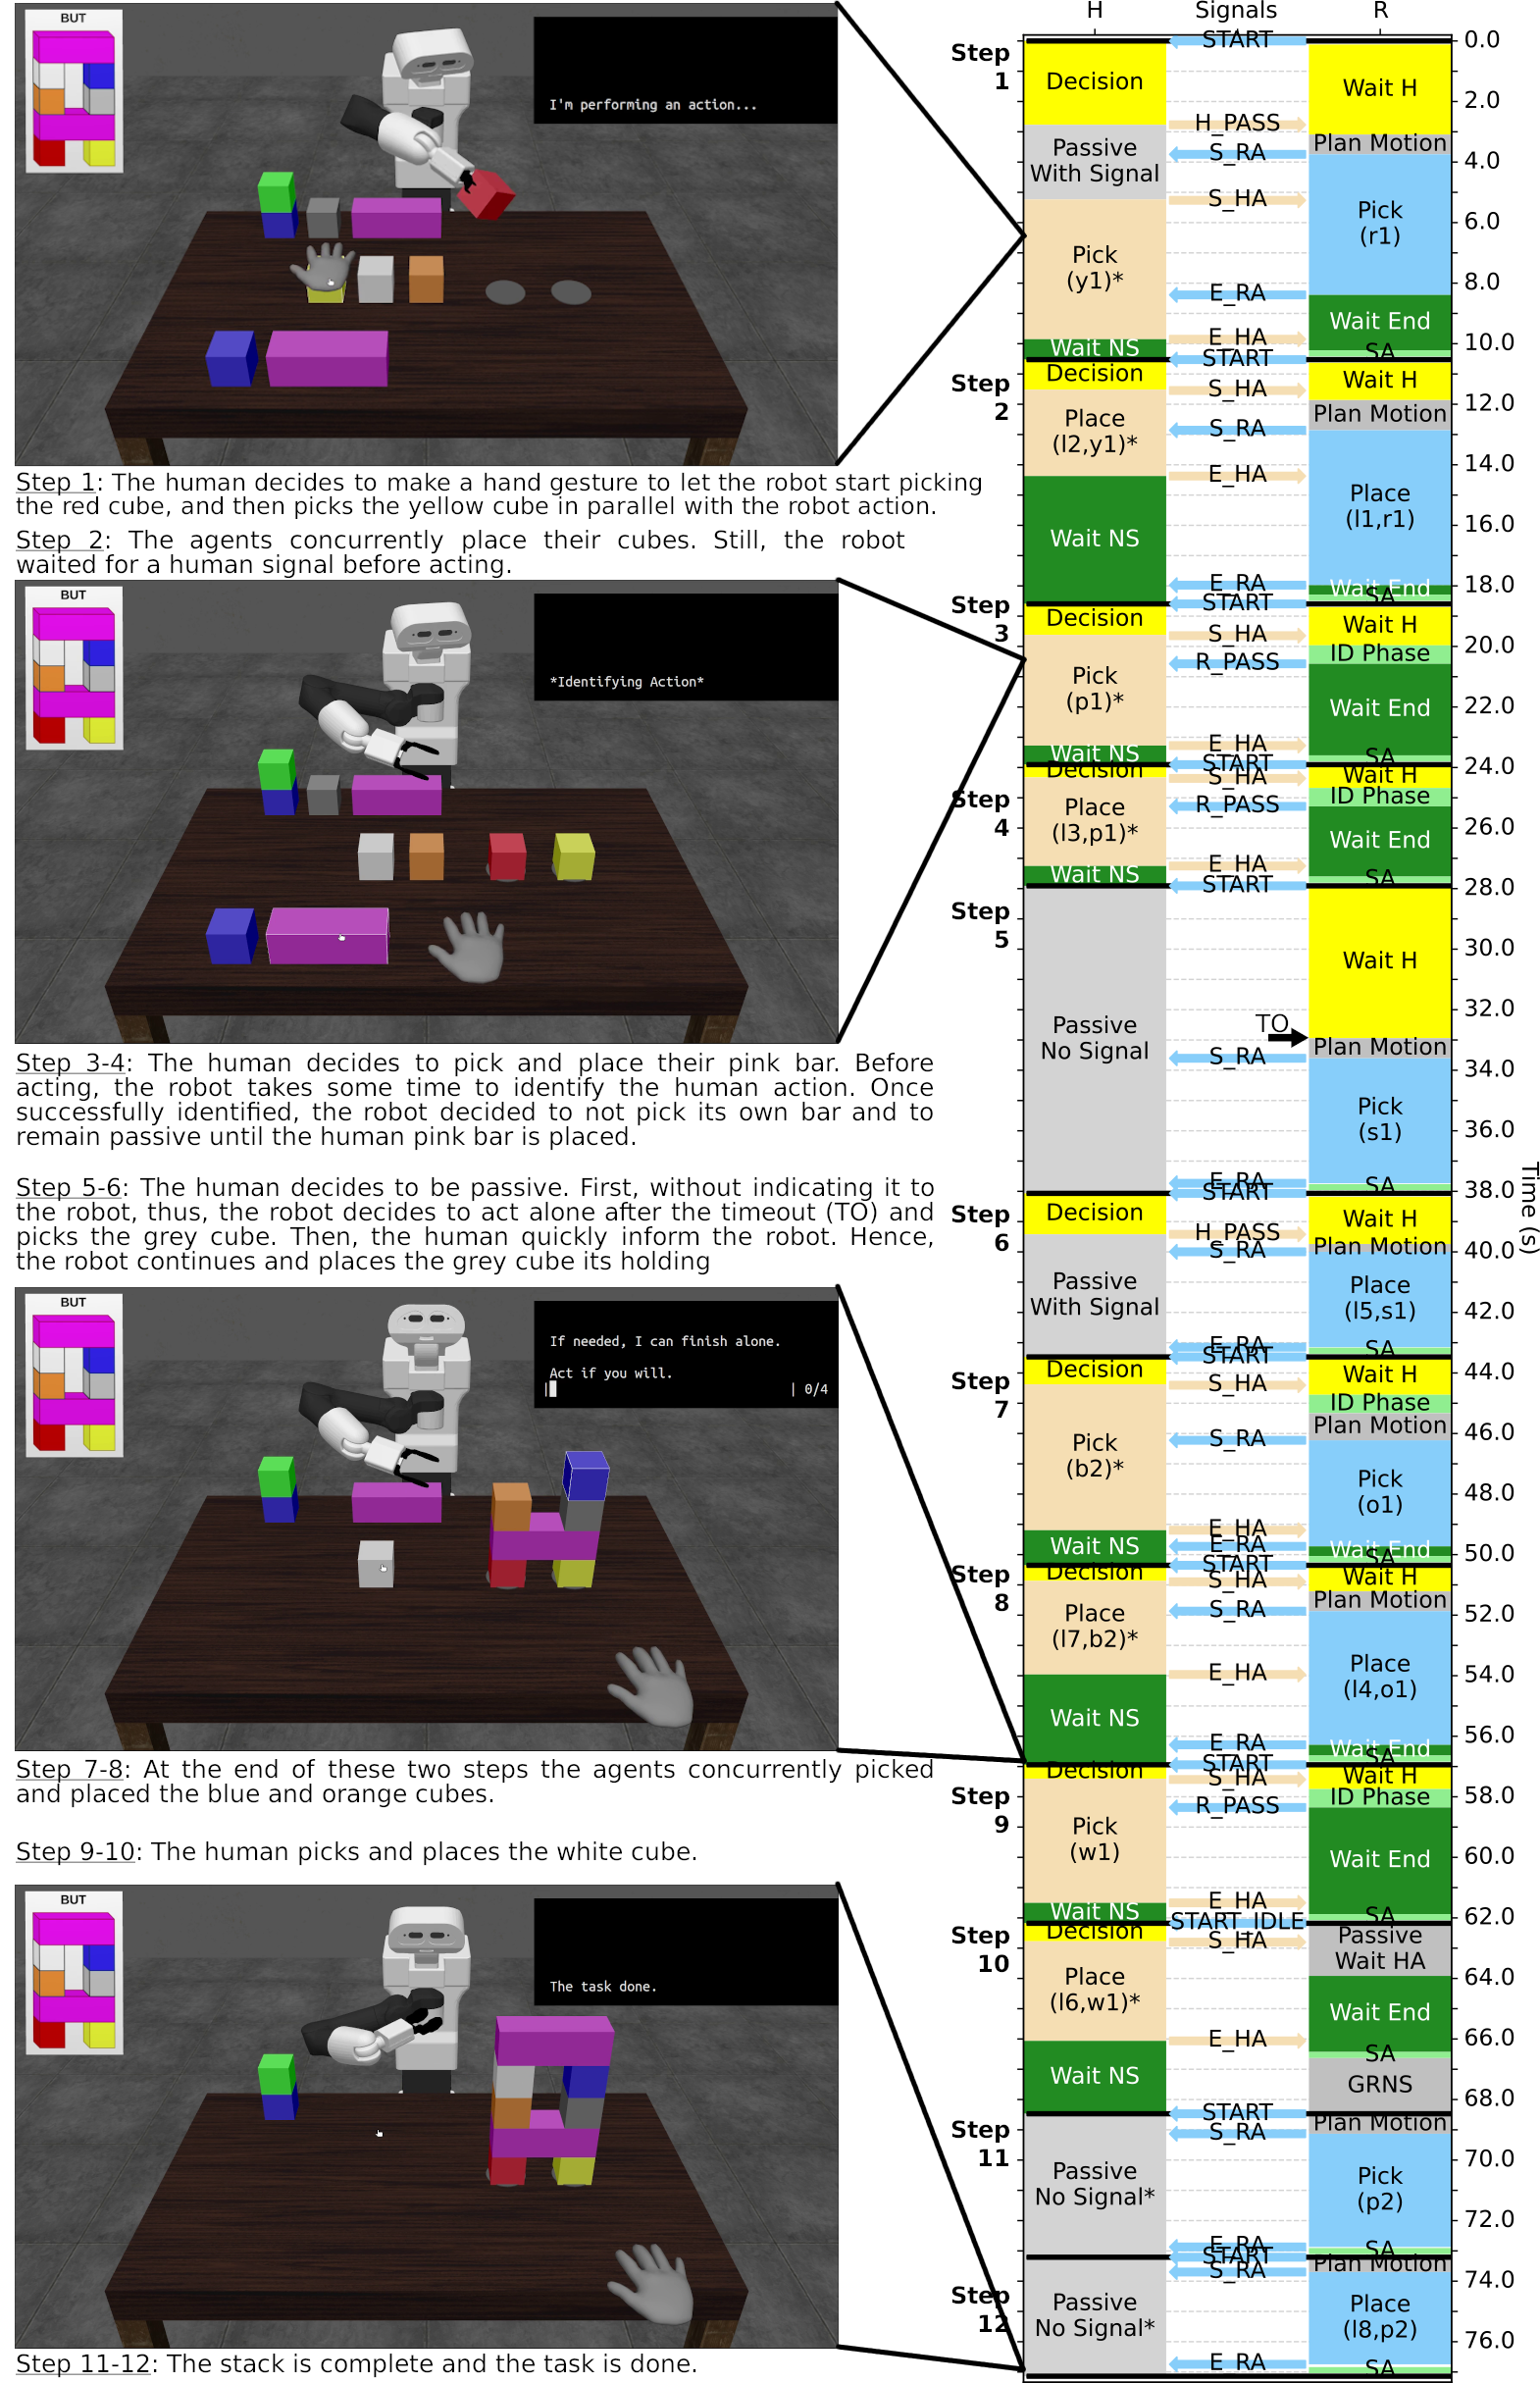
\includegraphics[height=0.97\textheight, keepaspectratio]{Chapter5/last_timeline.png}
    \caption{Complete execution timeline commented.}
    \label{fig:timeline_example}
\end{figure}

In this execution example, according to the extracted metrics, the task has been completed in $77.14s$ in $12$ steps. The average human decision time is $1.00s \pm 0.69s$ with $max=2.77s$ and $min=0.42s$. The human waited on average for the start of the next step during $1.68s \pm 1.28s$. There were $8$ human actions with an average duration of $3.67s \pm 0.72s$. According to the objective/preferences to finish the task as fast as possible, the human acted $9$ times optimally out of $12$ steps (optimal ratio$=75\%$). Indeed, the human agent purposely decided to be passive during steps 5 and 6, but they could have picked the orange cube in parallel to complete the stack faster. In this example, the task description forbids agents from picking cubes in advance. They must be able to immediately place a cube in the stack to pick it. This rule is detailed and justified later in the next chapter \ref{sec:study_protocol}. Hence, in step 9, the human picked the white cube, but the robot could not pick the bar until the white cube was placed. Thus, the human could have let the robot place the white cube to reduce their effort without slowing the task.
There were $8$ robot actions with an average duration of $3.97s \pm 0.69s$. Overall, the robot took $5.25s$ to plan its arm motions. 



\ifdefined\included
\else
\setcounter{chapter}{5} 
\dominitoc
\faketableofcontents
\fi

\chapter{User Study to evaluate an integrated plan and execution scheme in simulation}
\chaptermark{User Study evaluating our approach}
\label{chap:6}
\minitoc

\chapabstract{
This chapter presents a user study validating the approach proposed in Chapter~\ref{chap:4} using the simulator described in Chapter~\ref{chap:5}. For this purpose, several scenarios have been designed using a BlocksWorld task, and human participants were asked to collaborate with the simulated robot to evaluate its behavior. We compared our approach with a baseline behavior where the robot always imposes its decisions on the human. Using objective and subjective metrics, this study shows that our approach performed significantly better than the baseline. 
}

\section{Introduction}

To validate the approach presented in the previous chapter we conducted a user study on more than twenty participants. The purpose of this study is two-sided. 
First, we want to validate our overall planning approaches based on the proposed Model of Execution, and thus, show how it allows successful collaboration with a human. 
Secondly, we want to validate the Model of Execution itself, that is, showing how it allows the human to always be the leader and able to decide while the robot follows concurrently. We use a simple baseline to compare the Model of Execution with, and we show how our model allows to better satisfy human preferences and thus is preferred. 

We decided to conduct this study in simulation for various reasons. First, one of our assumptions is that all actions should roughly have the same duration. However, real-life robots are slow and not very reactive. Those aspects may bias the results of our study which is focused on decision-making. Secondly, simulation allows several simplifications that are acceptable for study. Collision with the cubes has been disabled to make the robot faster both in planning and executing its arm movements. In addition, simulation allows having a perfect perception of the environment. In a real-life experiment, perception errors may occur leading to replan, and thus slower execution, or even wrong decisions. Moreover, our model assumes that both agents synchronize after each step. Hence, it was easy in simulation to prevent the human from acting too soon and synchronize automatically their actions. In a real-life scenario, we couldn't physically prevent the participant from acting. This would imply a heavier training process for the participants to avoid desynchronizing with the robot. In practice, an additional execution supervisor should be developed to permit desynchronizing as long as they are not too big, and hence, prevent the system from crashing. This would require a significant technical effort to implement.

To conduct this study I developed a dedicated interactive simulator using a Tiago robot. In addition, the automaton described by the MoE has been implemented and integrated with the simulator to provide a proper execution and supervision scheme. Eventually, through carefully designed scenarios and using a shortened version of the PeRDITA questionnaire~\cite{devin_evaluating_2018} we gathered the feelings and impressions of the participants regarding the different robot behaviors. We also recorded logs from each executed scenario allowing us to draw a timeline of the execution and compute objective metrics for each scenario among which can be found: the time to complete the task, the human decision time, or the time for the human to be free. Several relevant facts and conclusions can be extracted from the collected results and are discussed in this chapter.

This chapter is organized as follows. First, the interactive simulator functionalities and operations are described. Then the methodology of the user study is provided along with anonymous information on the participants. After, the results obtained are presented and then discussed, validating the proposed hypothesis.

****

why simulation: HRI rebuttal: we rely on a reactive execution, real life robot are slow and not very reactive, may have perception errors, thus may bias our results focused on decision making.

Thus, we developed an interactive simulator running robot policies generated as explained the Chapter~\ref{chap:4}. Then, we conducted a user study using this simulator.

The purpose of this study is two-sided. First, we want to validate our overall planning approaches based on the proposed Model of Execution, and thus, show how it allows successful collaboration with a human. Secondly, we want to validate the Model of Execution itself, that is, showing how it allows the human to always be the leader and able to decide while the robot follows concurrently. Compared to a simple baseline, we also want to show how this model allows to better satisfy human preferences and thus is preferred. 

This chapter is organized as follows. First, interactive simulator functionalities and operations are described. After, the study protocol is presented as well as some analysis of the participants. Eventually, the obtained results are presented and discussed.

% *****

% Objective of the study is to validate the following:

% \begin{itemize}
%     \item \textbf{Overall planning and the use of Model of Execution during planning}: Always reach the goal, with different preferences, no need of prior negotiation, overall positive interaction, simple, use of MoE allows to explore all possible execution traces and complete the robot policy allowing human free to choose any action (OptimalRatio < 1.0) while still having a reactive robot, step synchronization questionable (sometimes liked, helps participant. Sometimes a bit lost in the step, however still ok.), real scenario should use additional execution supervisor allowing step superposition.
    
%     \item \textbf{Use of Model of Execution during execution}: The MoE describes how the robot always acts in a concurrent and compliant manner with the human. This allows the human to always (at every step) be in control. By using a mirror baseline where the robot always takes the lead instead of being the follower, we show that having the robot as a follower is preferred (H feels in control) and allows for better satisfying human preferences. The drawback of this approach is that currently, the robot is always a follower, making it slower since it always waits for the human to do something to adapt and act. Given to good results of the RF (with correct estimation) the question arises of trying to mix both approaches, having a robot that is by default a follower but sometimes takes the lead to be faster (when no risk of conflict?)
    
%     \item \textbf{Neither HA-planning nor compliant execution are sufficient alone}: Indeed, when the robot follows the HF regime with an incorrect estimation of human preferences the human can ``impose'' their decisions on the robot which will adapt, and thus, the human can satisfy their preferences anyway. However, in such scenarios, the human usually have one chance to impose their decision. Hence, if they are distracted the robot will eventually act in a not desired way which can lead to negative interaction. This can be observed with some participants either getting confused or distracted, and this didn't happen when the robot had a correct estimation of human preferences. Hence, it is important to have both a pertinent robot policy/plan selection complemented with an adaptive and compliant execution to have the best interaction possible.
    
%     \item \textbf{Not investigated in this work but,} our approach has been designed to allow specifying online new human preferences, updating the whole robot policy to satisfy the new given preferences. This allows either the human to directly specify their intents and preferences to the robot, or, an external process estimating online the human preferences.
% \end{itemize}

% The goal is to validate our approach presented in the previous chapter and justify the following. We believe that the robot should plan its actions with a compromise of optimizing the task efficiency, maximizing social criteria and satisfying human preferences while collaborating with humans. However, satisfying those social criteria is challenging since they cannot be accurately quantified. Especially for human preferences which can fluctuate a lot depending on their mood and context. That is why we believe, in addition to planning the best course of action using all these criteria, it is relevant or even mandatory for the robot to adapt and be compliant with human online decisions and actions. 

% Hence, this study aims to show two main things. First, during execution, the robot should adapt and be compliant with the human actions. Indeed, it is hard to accurately estimate human behavior and preferences. In case of incorrect estimation, having a compliant robot helps to satisfy the human preferences (HF vs RF, better answers). Also, the human may act differently than expected by the robot, the latter should be able to allow this and comply with it (ratio\_h\_optimal < 1.0).
% Secondly, the study validates our overall planning (and execution?) approach. The goal is always solved. The collaboration is always useful (more or less) and not so low (positive). 
% Third, we can also say that despite having to be compliant online, it is very beneficial to plan correctly beforehand the robot actions. 

% \textbf{TODO: GOAL of the study is to validate two things. First, our overall planning approach. Secondly, the HF model of execution. 1) Should see that overall even when wrong RF the robot isn't so bad, still useful, simple, competent, responsive. Could do better and a bit frustrating but still ok to accomplish the task. 2) Should see that HF is significantly preferred and results in more acceptable and appreciated behavior : Adaptive, Appropriate, Accommodating, Positive.}

\section{Related work}

\subsection{Questionnaires}
Many questionnaires are used in the field of HRI. The main ones are listed here: GodSpeed, HRIES, PeRDITA, RoSAS, and Trust Perception Scale-HRI. 

Each questionnaire has specificities and helps to measure certain aspects of the robot. Many include appearance items to evaluate the look of the robot. Since our focus is on robot decision-making, we decided to base our questionnaire PeRDITA. Indeed, this questionnaire has been designed to evaluate the pertinence of robot decisions in a Human-Robot Joint Action Context, which is exactly our case. Yet, the full questionnaire is a bit heavy and also covers communication which isn't our topic in this work. 
That is why we decided to shorten the questionnaire by removing the section on communication and a few redundant items. Redundant items are helpful to evaluate the consistency of a questionnaire and this has already been done in~\cite{devin_evaluating_2018}. Hence, to avoid participants getting bored and lost by filling out the whole questionnaire after every scenario we kept 12 items covering the following dimensions: robot perception, interaction, collaboration, and acting.



\section{Study protocol} \label{sec:study_protocol}

Methodology: 
Initial demographics questionnaire to identify potential individual difference ratings. Then, presentation instructions/text. After, familiarized with the simulator through an interactive tutorial. Eventually, the six scenarios in randomized order are experienced by the participant. After each scenario, the participant answers a shortened version of the PeRDITA questionnaire and logs about the execution are saved. Eventually, the participant is asked about their overall impressions regarding the interaction they had with the simulated robot, and they are asked which scenario they preferred the most and the least. The overall experiment takes about 35-40 min per participant. 

objective, participants, material, experiment design, procedure, measures

This section describes the objectives and protocol of this study.  



\begin{figure}
    \centering
    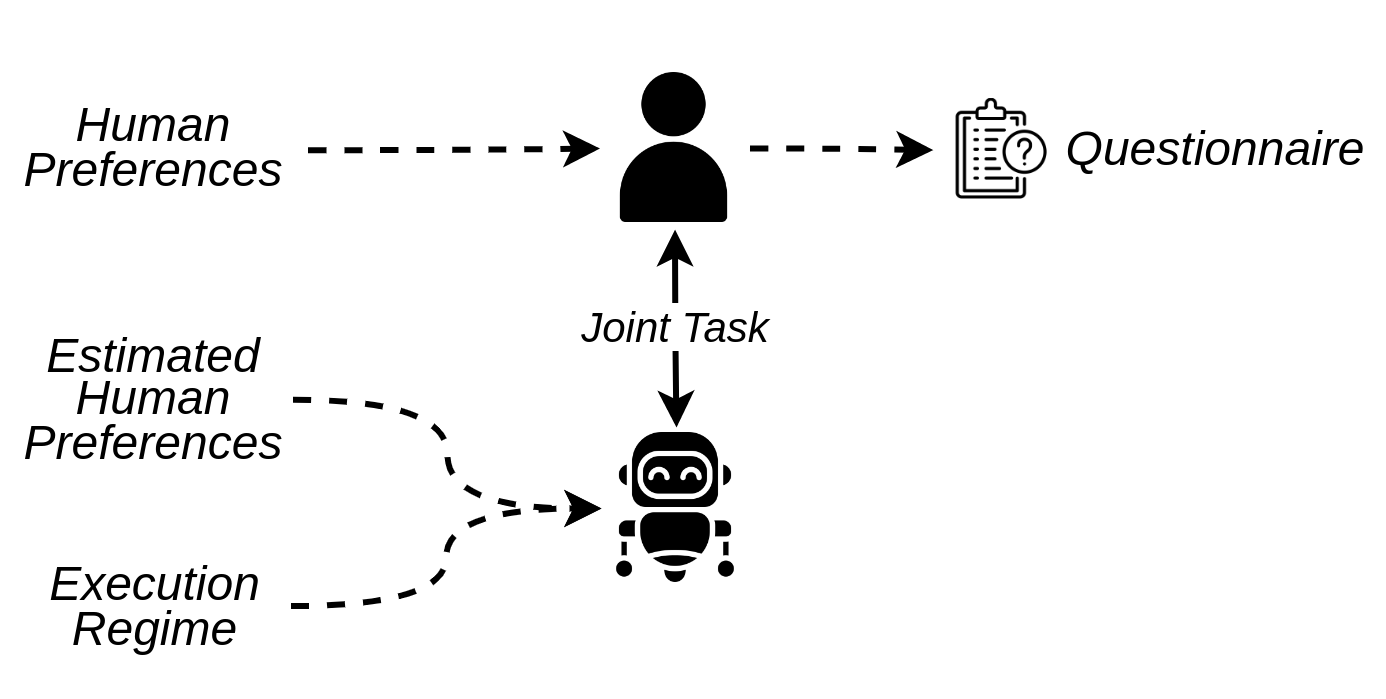
\includegraphics[width=0.8\textwidth]{Chapter6/UserStudyProcedure.png}
    \caption{A scenario of the User Study Protocol. Each participant goes through 6 scenarios and answers 6 questionnaires to evaluate each different robot's behavior}
    \label{fig:user_study_protocol}
\end{figure}




Through this study we want to demonstrate the benefits of using the model of execution described in the previous chapter~\ref{chap:4} in a collaborative context. We believe this model of execution is pertinent to be taken into account when executing and supervising a robot's plan. For the same reasons we based the policy generation of this model and aim to justify our choice and validate our approach.

In this study, each participant is made to collaborate six times with a simulated robot to achieve a shared task, each time is referred to as a scenario. The robot exhibits a different behavior in each scenario. After each scenario, the participant evaluate the robot's behavior through the PeRDITA questionnaire \cite{devin_evaluating_2018}.

Beforehand, every participant answers a few general/demographic questions and is familiarized with the simulator functionalities through an integrated tutorial. Only then they start the six consecutive collaborative scenarios, answering every time a questionnaire to describe the interaction. Eventually, every participant is asked to share their general feelings and impressions about the overall interaction with the simulated robot, and they are asked to tell which scenario they preferred the most and the least.

\begin{figure}
    \centering
    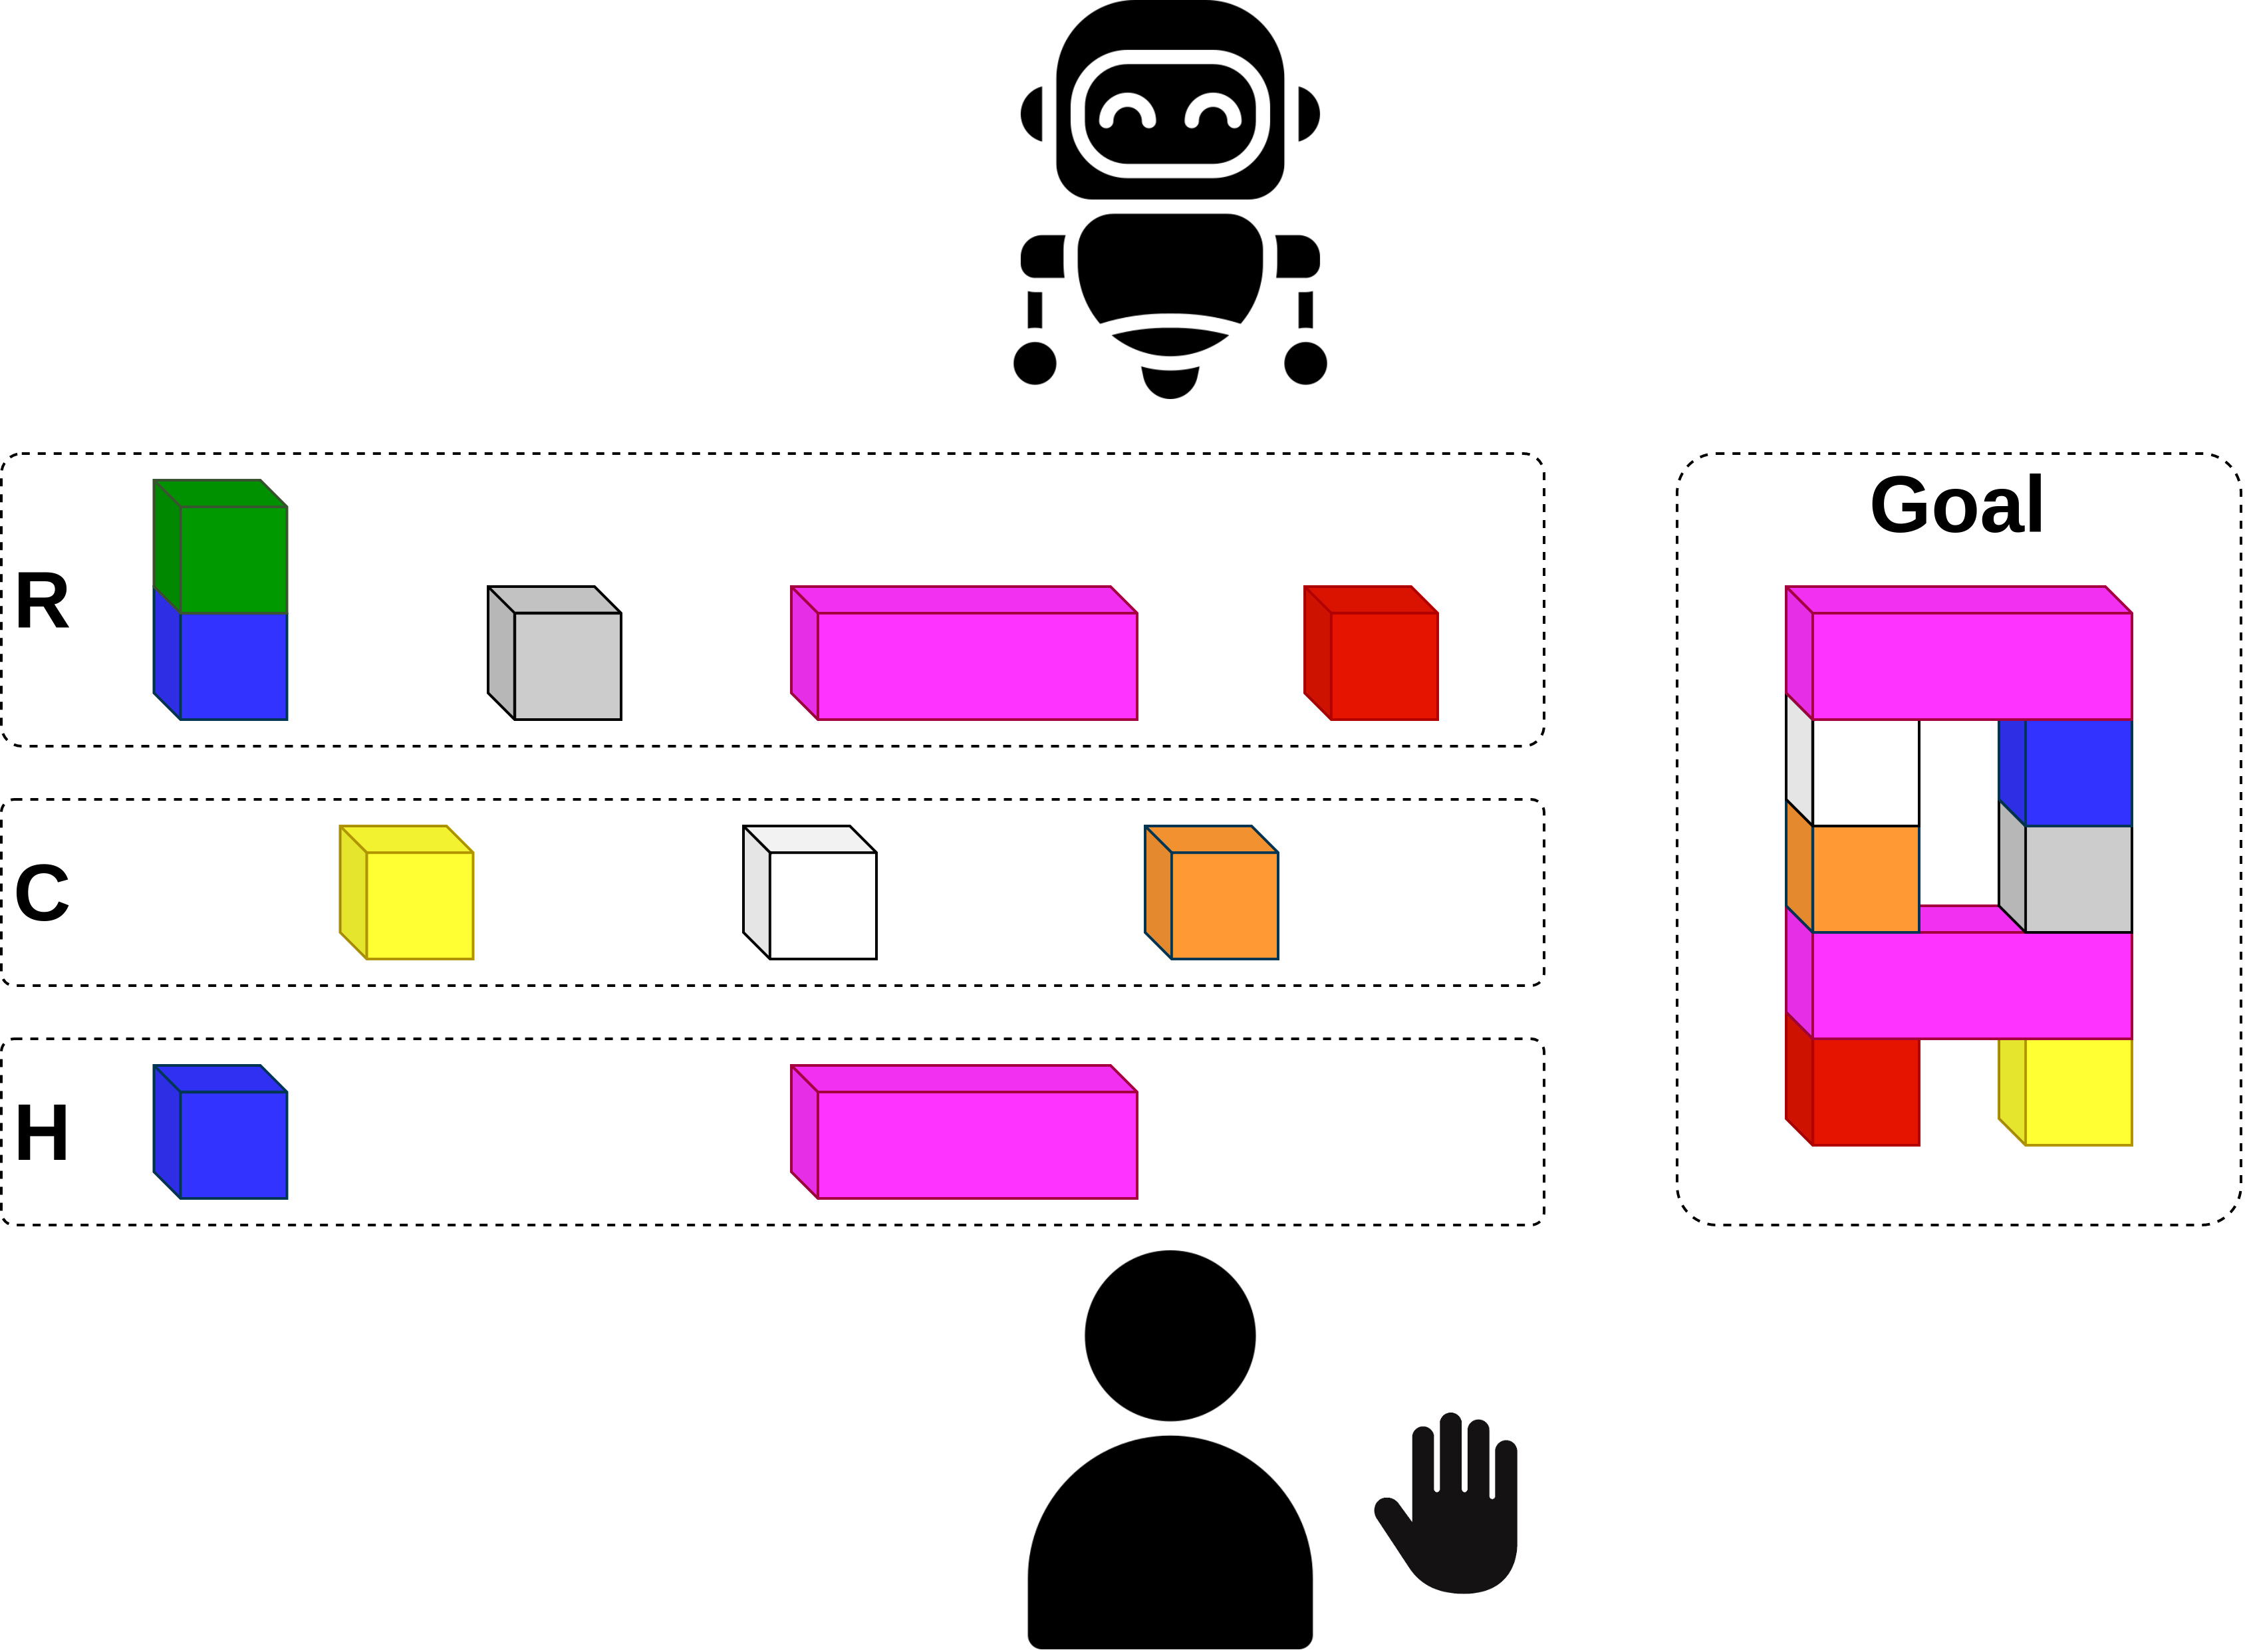
\includegraphics[width=0.8\linewidth]{Chapter6/task_description_study.png}
    \caption{Description of the shared task to achieve in the study.}
    \label{fig:task_description_study}
\end{figure}

We now provide details about the task, the scenarios and how the different robot behavior are generated. 
The shared goal, which is stacking the cubes to match the given pattern, remains the same in all scenarios. The cube disposition on the table also doesn't change either. The task description is depicted in fig~\ref{fig:task_description_study}. For this problem, our planning approach generated a solution graph with 700 PStates/nodes leading to 6 different final states/leaves. This solution graph comprises $6839430$ different possible courses of action. The length of the plans is about $19.77 \pm 1.59$ steps, with a minimal length of $11$ steps and a maximal length of $23$ steps.

To progress in the task, the agents can perform three different primitive actions which are the following: \textit{pick} a cube, \textit{place} a cube in the stack, or, \textit{drop} a cube back on the table.
These actions have a few preconditions, more or less intuitive, that are communicated and experienced by the participant during the integrated tutorial.
First, one can \textit{place} a cube if they hold the cube, and if the targeted location is free and supported. That is, the cubes directly below the targeted location must be placed before being able to place a cube in the targeted location.
Secondly, one can only \textit{pick} a cube from their respective reachable zones of the table, i.e., Human and Center zones for the human, and Robot and Center zones for the robot. Also, one can only pick a cube if it can be placed immediately. Thus, one cannot pick a cube ``in advance'' and has to wait to its placement condition to be true before picking it up. For instance, both pick bars can only be picked up after the yellow and red cubes have been placed. This rule helps to create interaction conflicts serving the purpose of this study. Moreover, although the participants find this not intuitive they get used to it really fast and this feeling seems to be significantly reduced along the experiment.
Third, one can \textit{drop} a cube back on the table only if they hold it and if it cannot be placed.

For each scenario the participant is given instructions regarding how to solve the task. The participants are asked to consider these instructions as their own choice and preferences regarding the task resolution, and thus, to act accordingly while collaborating. The instructions at each scenario are one of the two following.
On the first hand, the participant shall act in a way to finish the task as soon as possible. Here, it consists in trying to perform as many actions in parallel as possible to progress faster. These preferences are latter referred to as Task End Early (TEE).
On the other hand, the participant shall act in a way to be freed as soon as possible. That is, they should finish their mandatory part of the task as soon as possible, so they could leave and let the robot finish alone. Here it consists in placing the pink bar from the Human zone as soon as possible. These preferences are latter referred to as Human Free Early (HFE).
On its side, the robot doesn't directly have access to these instructions/preferences, they are only estimated. Hence, for each scenario, the robot is given a more or less accurate estimation of the human preferences that are communicated to the participant. Note that the participants aren't aware that the robot has an estimation of their preferences, neither that this estimation can be inaccurate.
This way, we created three scenarios with different pairs of human preferences and associated estimation. In the first pair, the human shall finish the task early and the robot has a correct estimation, i.e., the robot's policy is helping the human to finish the collaborative task early. In the second pair, the human preferences remain the same, but the robot estimation is incorrect. The robot is trying, mistakenly, to minimize the human effort. As a consequence, the robot tends to pick cubes that the human could pick, preventing the human from acting and making the task completion longer. In the third pair, the human shall free themselves early, but the robot estimation is again erroneous. The robot will try to finish the task early while its priority is to place the first pink bar, which is conflicting with the given human preferences.

Additionally, in each scenario, the robot follow one of the two following execution regimes:
\begin{itemize}
    \item \textbf{Robot-First (RF)}: the robot always initiates actions first, and the participant take action afterwards.
    \item \textbf{Human-First (HF)}: the robot always lets the participant take the initiative, and then acts.
\end{itemize}
The \textit{Human-First} execution regime corresponds to the Model of Execution described in the previous chapter. At each step, the robot waits for the human's decision and will execute the best action that complies with it. The human always start acting first and the robot follows. On the other hand, the \textit{Robot-First} regime corresponds to a naive and straightforward policy execution where, at each step, the robot directly starts executing the overall best robot action given by the policy. The robot always starts acting forcing the human to comply. The \textit{Robot-First} regime serves as a baseline to evaluate the proposed \textit{Human-First} regime, described by our Model of Execution and used in the policy generation.
Eventually, we associate each of the three previous pairs of preferences and estimation with one of the two different execution regime. As a result, we obtain six different scenarios with six different robot behaviors named in table~\ref{tab:scenario_names}.

\begin{table}
    \caption{Name of the six scenarios. 
    Columns represent the preferences/estimation pairs and the rows correspond to the execution regimes.}
    % \vspace{-15pt}
    \begin{center}
    \begin{tabular}{c|c|c|c|}
        \cline{2-4}
                                                & Pair A        & Pair B            & Pair C\\
                                                & TEE: correct  & TEE: incorrect    & HFE: incorrect\\
        \hline
        \multicolumn{1}{|c|}{Human-First}       & S1            & S3                & S5\\
        \hline
        \multicolumn{1}{|c|}{Robot-First}       & S2            & S4                & S6\\
        \hline
    \end{tabular}
    \end{center}
    \label{tab:scenario_names}
\end{table}

Note that our goal is to evaluate and compare the different robot behaviors. However, at the beginning, the participants don't have any references to compare with which can influence their answers in the very first scenarios. One solution is to ask the participants to answer all six questionnaires at the end, after being familiar with the six scenarios. We consider that this option demands a too heavy mental workload to recall accurately each specific scenario, and may bias the answers. As a consequence, we decided to ask the participants to answer the questionnaire after each scenario as a draft. During the experiment, they can rectify their answers to match more accurately their feelings. At the end, using the drafts, they share their final answers for each scenario. We believe this process allows to more accurately gather the feelings of the participants. Moreover, the ordering in which the participants encounter the scenarios is uniformly randomized to prevent any order effect. 


\begin{table}[h]
    \footnotesize
    \begin{tabular}{ccc}
    \hline
    \textbf{Dimension}                         & \textbf{Question}                                                                                                                     & \textbf{Item}             \\ \hline
    \multirow{3}{*}{\textbf{Robot perception}} & \multirow{3}{*}{\begin{tabular}[c]{@{}c@{}}In your opinion,\\ the robot is rather:\end{tabular}}                                      & Apathetic/Responsive      \\
                                               &                                                                                                                                       & Incompetent/Competent     \\
                                               &                                                                                                                                       & Unintelligent/Intelligent \\ \hline
    \multirow{3}{*}{\textbf{Interaction}}      & \multirow{3}{*}{\begin{tabular}[c]{@{}c@{}}In your opinion, the interaction\\ with the robot was:\end{tabular}}                       & Negative/Positive         \\
                                               &                                                                                                                                       & Complicated/Simple        \\
                                               &                                                                                                                                       & Ambiguous/Clear           \\ \hline
    \multirow{3}{*}{\textbf{Collaboration}}    & \multirow{3}{*}{\begin{tabular}[c]{@{}c@{}}In your opinion, the collaboration\\ with the robot to perform the task was:\end{tabular}} & Restrictive/Adaptive      \\
                                               &                                                                                                                                       & Useless/Useful            \\
                                               &                                                                                                                                       & Inefficient/Efficient     \\ \hline
    \multirow{3}{*}{\textbf{Acting}}           & \multirow{3}{*}{\begin{tabular}[c]{@{}c@{}}In your opinion, the robot\\ choices of action were:\end{tabular}}                         & Inappropriate/Appropriate \\
                                               &                                                                                                                                       & Annoying/Accommodating    \\
                                               &                                                                                                                                       & Unpredictable/Predictable \\ \hline
    \end{tabular}
    \caption{PeRDITA Questionnaire: Participants have to place themselves between the two antonym items in a scale of 7.}
    \label{tab:perdita_questionnaire}
\end{table}

The questionnaire filled by the participants after each scenario is a shorten version of the PeRDITA questionnaire, and its items are gathered in table~\ref{tab:perdita_questionnaire}. 
In addition to the questionnaires, for each scenario, the interactive simulator produces logs from which we extract several metrics and an overall timeline of the execution. The timeline depicts the activities and actions of each agent along the task progression. The subjective measures done through the questionnaire are complemented with the objective metrics extracted such as the duration to complete the task, the number of human actions, the total duration of human inactivity, and more. 


There are a few restrictions on the actions that can be performed. First, an agent can only pick cubes that can be placed immediately. This means that agents cannot pick cube in advance to anticipate each other's actions. Allowing such behavior could generate a very interesting scenario. However, here we want to purposely generate some conflicts to evaluate the robot's behavior and reactions. Without this restriction, the agents would have too much flexibility in their actions and decisions which makes it harder for the conflicts to happen.  
Additionally, when holding a cube, the agents can only place the cube in the stack on back to its original place. As a result, the agents cannot displace the cube on the table to make them reachable to the other agent. This restriction has been added for the same reasons as the first one and simplifies the conflicts generation. 

\begin{figure}
    \center
    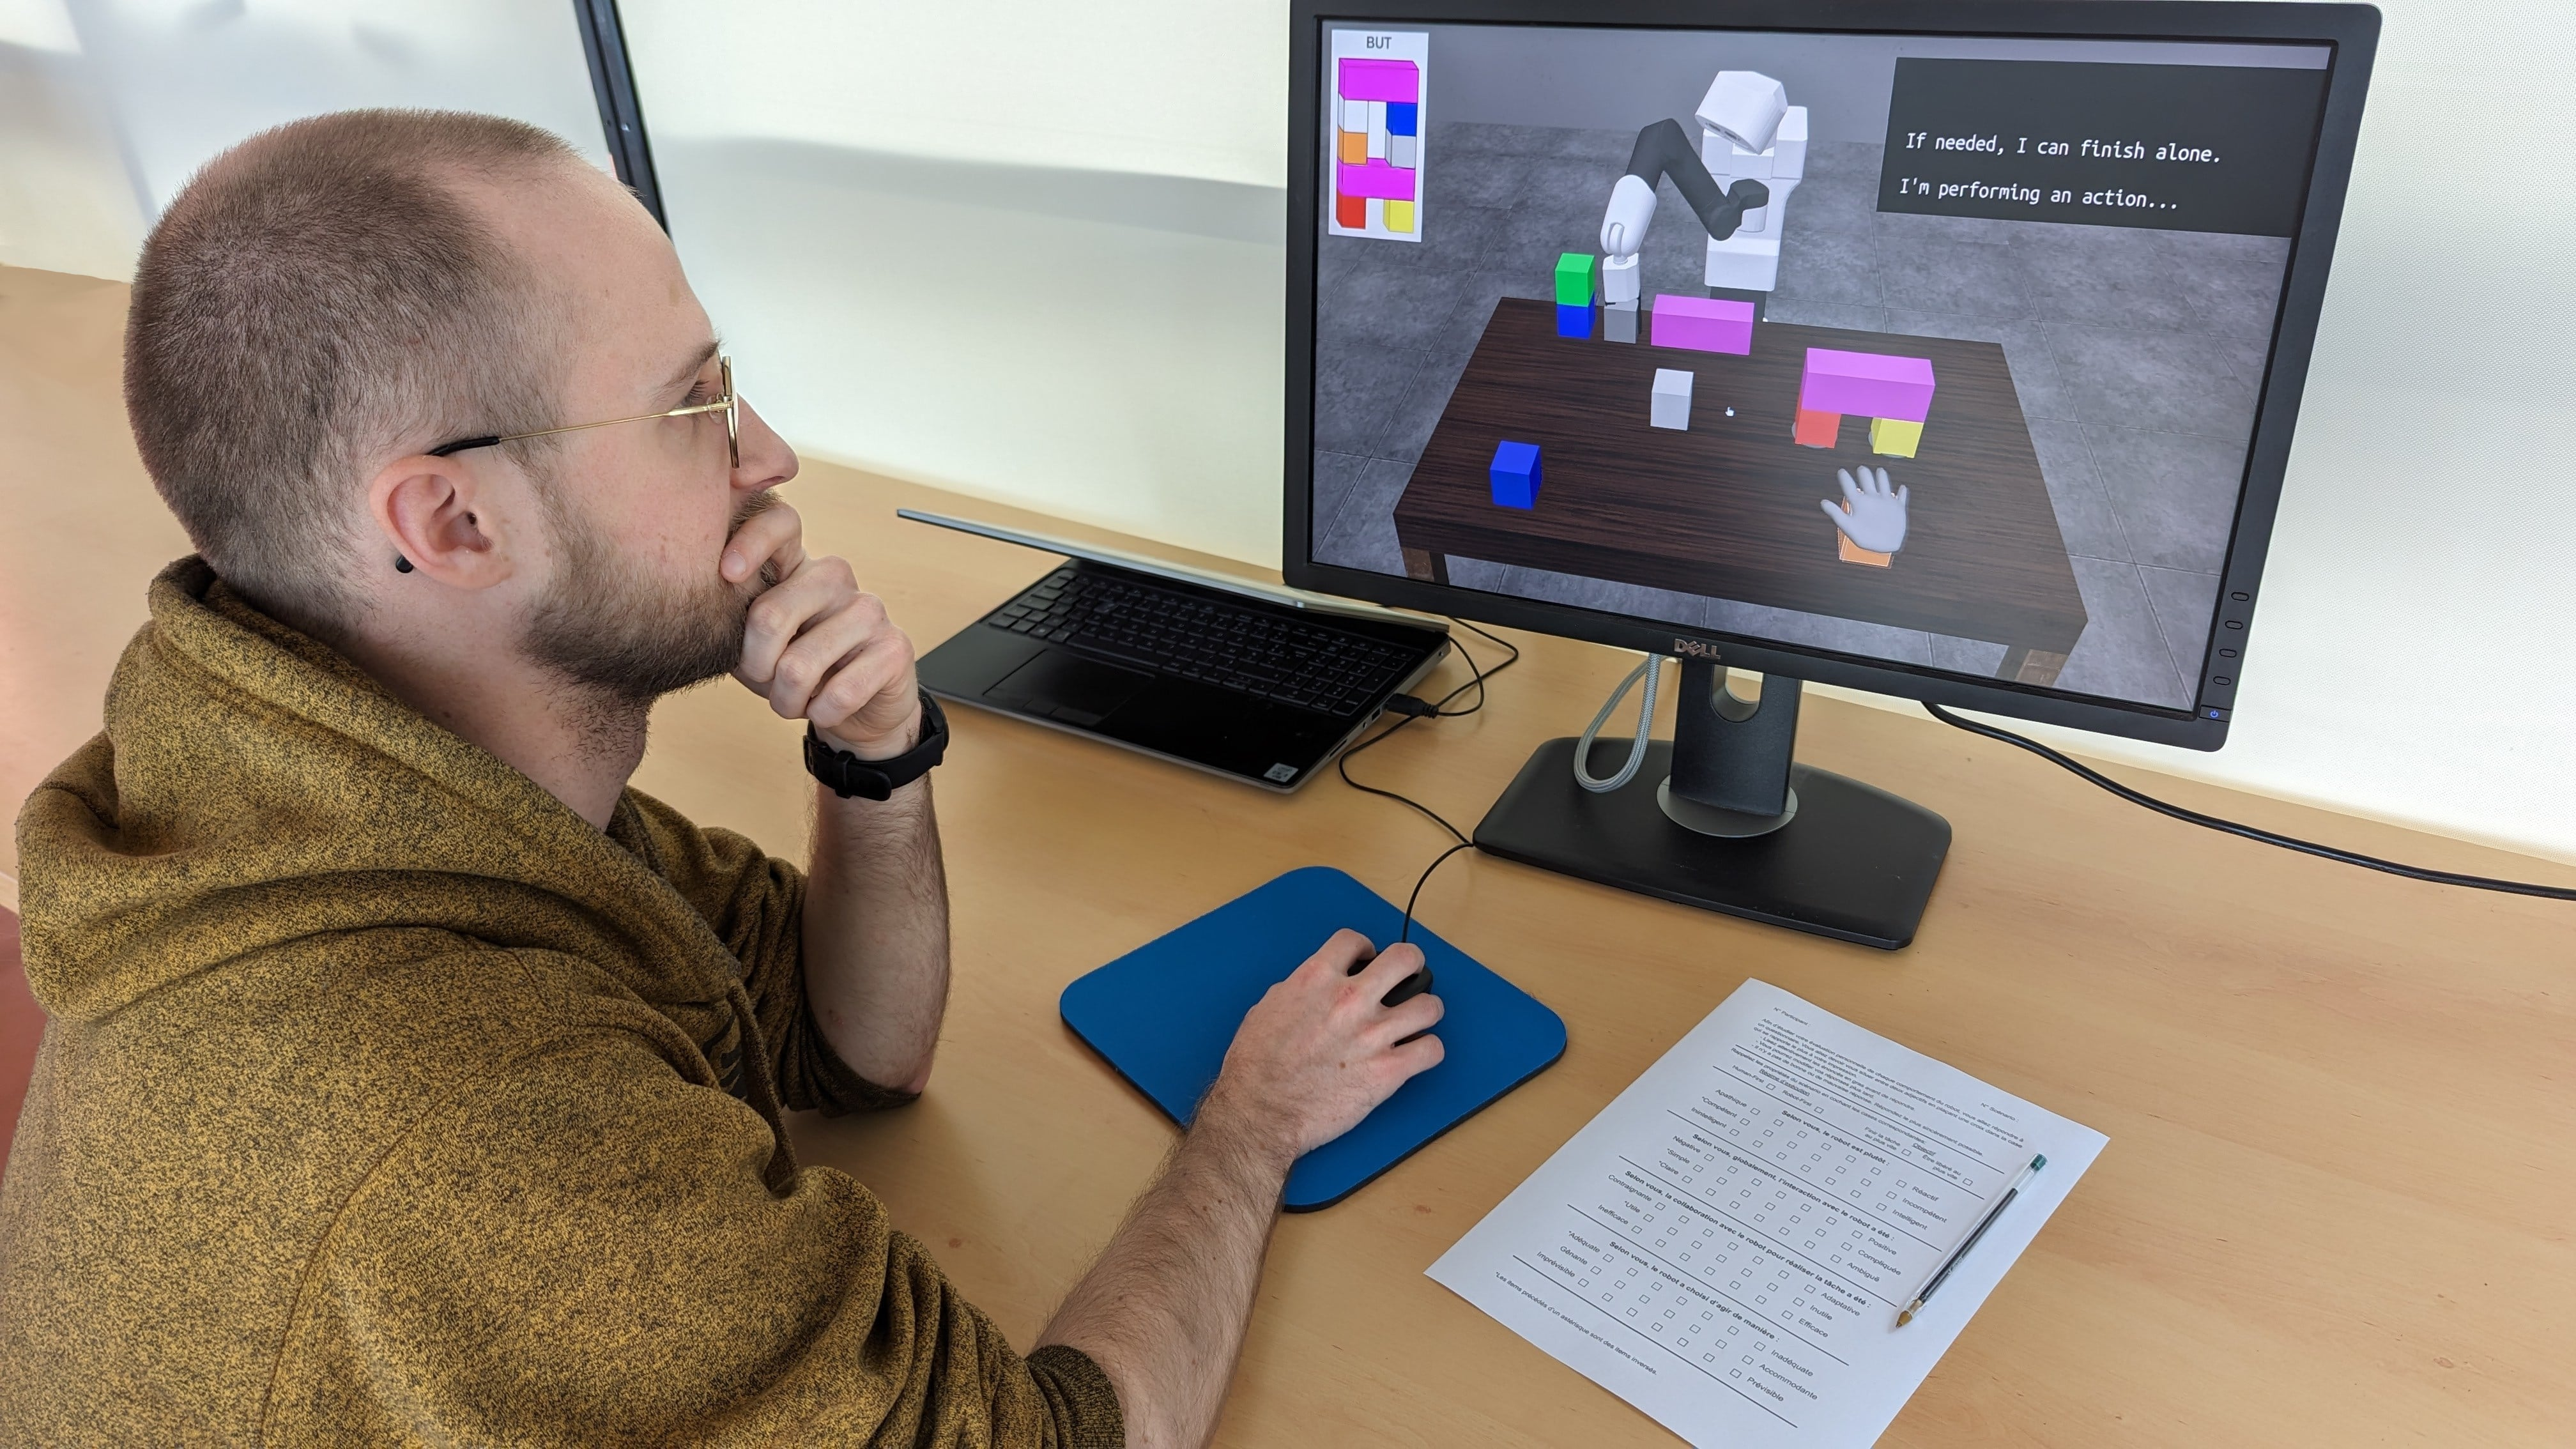
\includegraphics[width=\linewidth]{Chapter6/participant-min.jpg}
    \caption{One scenario execution where a participant is collaborating with the simulated robot using the mouse. Once the task is completed, the participant is asked to fill the questionnaire on the desk with a pencil to transcribe their impressions.}
    \label{fig:participant}
\end{figure}

The participants were collaborating with the robot using a mouse. The simulation was run on a laptop connected to a bigger screen allowing participants to see clearly the simulated environment. After each scenario, participants answered the printed questionnaire using a pencil. Figure~\ref{fig:participant} depicts the execution of a scenario where the participant collaborates with the simulated robot using the mouse. Once the task is completed and the scenario is over, the participant is asked to fill out the printed questionnaire on the desk with a pencil. For each scenario, a new paper sheet is provided to the participant. 

\section{Participants}

This section shares and analyzes some information on the participants.

\textbf{TODO: provide info} number, age, ext, familiar with R tech, vision of robotics

\section{Study results}

In this section, we analyze the results of the study with first some technical comments regarding the experiment. After, we analyze the results obtained from the execution logs. Then, we discuss the questionnaire's answers. Finally, we discuss the participant's comments regarding the experiment. Note that all the numeric results of the study are given in appendix~\ref{ap:study}, including questionnaire answers, execution metrics, comments, and scenario preferences. 

\subsection{Technical comments}

Numerous scenarios were executed in the simulator to conduct this study. More precisely, $150$ scenarios were executed and a total of $1914$ steps were executed. It is interesting to share a few technical comments about how those executions.

To begin with, very few technical issues or crashes occurred during the study.
About 2 or 3 crashes were due to a failure in the HMI that had happened when participants clicked at a very specific instant. I wasn't able to identify the origin of the issue, but this only happened a few times considering that $1048$ human actions were performed during the whole study. This means that $0.29\%$ of the human action failed. 
Then, about 4 to 6 crashes occurred due to a failure of the robot arm motion controller. The arm motions were planned successfully but the controller failed to execute the planned trajectory in the simulator which led to a crash of the controller, freezing the robot. This kind of failure was specific to the MoveIt framework and I couldn't find a solution to them. But again, those issues were quite rare considering that the robot performed a total of $1586$ actions during the study. This means that $0.38\%$ of the robot action failed. 
Overall, less than 10 scenarios crashed during the study which is less than $6\%$ of failures. 
In practice, recovering from a crash was quite easy and fast. After a brief intervention of less than $30s$, the participants were able to start again from the scenario that crashed. Sometimes, this implied the participants to repeat a large part of the crashed scenario which affects the participant impression (less novelty effect) but none significantly changed their actions when repeating such a scenario.


On the other hand, it is worth mentioning and discussing the durations of the different processes run by the robot.
At every step, the robot has to decide which action to perform, move its head, plan its arm motion, and move its arm. First, the decision time of the robot is negligible because it is given by the policy computed previously by our planning approach. Before every step, the robot identifies the current state. Given a state, the policy dictates the robot which action to perform, including if the human action must be identified first. Since all this is precomputed, the decision time is negligible. 
Head motions are also not demanding, and their execution occurs in parallel with the other robot processes, hence they can be neglected.
However, planning the robot's arm motions is heavy computing and takes about $0.56s \pm 0.28s$. Notice that the standard deviation is quite high, about half of the average value. Indeed, the motion planning is based on algorithms using randomized exploration which makes the solving time random, sometimes begin very fast ($min \approxeq 0.001s$) and sometimes quite slow ($max = 5.37s $). Yet, we were able to plan online the arm motion.
Eventually, the robot arm motion durations are about $4.09s$ (max=$9.09s$, min=$1.46s$) and will be discussed more precisely below

Additionally, since the task is quite simplistic, repetitive and deterministic, one could say that we could have pre-computed the robot arm motions in order to lighten the execution and avoid technical problems linked to motion planners. First, we insist on the fact that the arm motions failures were due to execution failure, not planning, thus it is unclear if pre-computed the trajectory would have helped regarding those failures. Doing so would certainly make the simulator less demanding in terms of computation power. But here we wanted to keep a generic simulator able to able any other task, thus, movements couldn't be pre-computed.

\subsection{Statistical assumptions}

Our data are close to following a normal distribution (checked using Kolmogorov-Smirnov, Shapiro-Wilk and Anderson-Darling tests). Thus, parametric tests can be applied, and we used both paired t-tests and Analysis Of the VAriance (ANOVA) with repeated measures to analyze the collected data, more precisely, to identify significant differences between different group of measures. 
In the last case, Bonferroni Post-hoc-Tests are performed to identify exactly which groups are significantly different from others.

It has been commonly assumed that a statistical test demonstrates a significant difference if a p-value lower than $0.05$ is obtained. However, obtaining a value lower than $0.001$ is desired. To make the p-values more legible the following standard notation is commonly used and will be used below:

\begin{align*}
    p > 0.05        & \Rightarrow ns ~ (\textrm{non significant})\\
    p \leq 0.05     & \Rightarrow * ~ (\textrm{significant})\\
    p \leq 0.01     & \Rightarrow ** ~ (\textrm{very significant})\\
    p \leq 0.001    & \Rightarrow *** ~ (\textrm{highly significant})\\
\end{align*}

Additionally, the value a metric $x$ will often be given in the following format including the average value $M$ and the associated standard deviation $\sigma$: $x = M \pm \sigma$.


\subsection{From execution logs}

This section is focused on analyzing the results obtained through the execution logs saved after each scenario. 

\subsubsection*{Preferences satisfaction (task completion time + time to be freed)}

\begin{figure}
    \center
    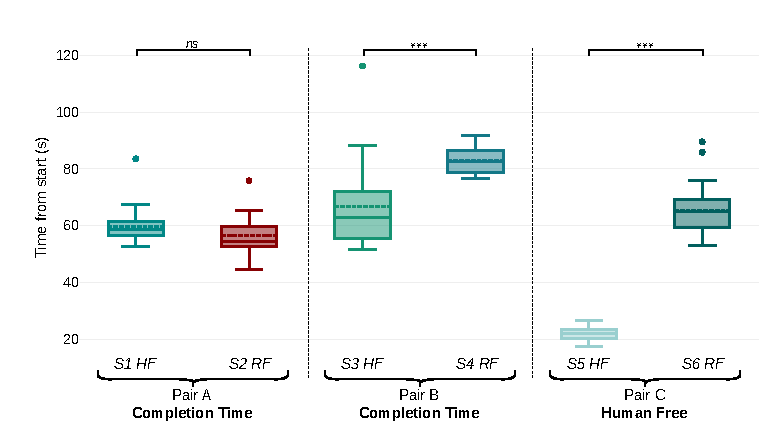
\includegraphics[width=\linewidth]{Chapter6/preferences_sastisfaction.pdf}
    \caption{Human preference satisfaction. According to the scenarios, it corresponds either to completing the task as fast as possible (Pair A and B) or being free as soon as possible (Pair C). Using t-tests for paired samples, we can identify in pair B and C the criteria of preferences is significantly better satisfied. In pair A, the difference isn't significant but the completion time is slightly shorter when using RF.}
    \label{fig:preferences_satisfaction}
\end{figure}

In this study, the human preferences consist of either finishing the collaborative task as soon as possible or being free as soon as possible while letting the robot finish alone. 
Thus, to evaluate how the human preferences were satisfied, we can measure in the first case the time to complete the task and in the second case the time after which the human can leave. 

Figure~\ref{fig:preferences_satisfaction} depicts through box plots for each pair of scenarios the corresponding relevant metric to evaluate the human preferences' satisfaction. We used t-tests for paired samples for pairwise comparison. For each pair, the tests for normal distribution suggest that the data does not significantly deviate from normality, and thus parametric tests such as t-tests can be conducted.

In Pair A, in addition to completing the stack the human wants it to be completed as soon as possible. The robot has a correct estimation of human preferences. The completion time using HF and RF are shown. The completion times in S1 and S2 are roughly similar with the respective values: $59.84s \pm 5.83s$ and $56.64s \pm 6.46s$. The completion time of Scenario 1 is higher than Scenario 2. However, a t-test for paired samples showed that this difference was not statistically significant ($p = 0.055$) and there was a small effect ($d = 0.4$) according to Cohen's \textit{d}~\cite{cohen1988concepts} (small effect = $0.2$, medium effect = $0.5$, large effect = $0.8$). Thus, the RF regime allowed the human to solve the task slightly faster than the HF regime, and thus, satisfy their preferences slightly better. 
In both scenarios, the collaboration goes smoothly, and the task is achieved without trouble.

In Pair B, the human still wants the stack to be completed as fast as possible, however, the robot has an erroneous and adversarial estimation of their preferences. This time the HF regime in S3 had lower values ($66.62s \pm 14.87s$) than the RF regime in S4 ($82.82s \pm 4.42s$). This difference is statistically significant ($p < 0.001$) and there was a large effect ($d = 1.07$). This indicates that in S4 the participants' preferences were significantly less satisfied than in S3. 
Indeed, in this pair, the robot erroneously thinks that the human wants to minimize their effort. Thus, the robot ends up trying to ``\textit{steal}'' cubes from the human to prevent them from acting, thus, minimizing their effort. With RF the human has no choice and cannot act most of the time, leading to a high completion time with a low standard deviation due to the restricted human choices leading to very similar executions. With HF the robot always acts compliantly in parallel right after the human. Hence, the human is able to pick the cubes they want and that the robot wants to pick, \textit{forcing} the robot to adapt and pick other cubes. This eventually leads to executions close to S1. However, if for any reason the human doesn't pick the cubes then the robot picks them preventing again the human from acting, explaining the high standard deviation. Comments about the feelings of the participants in each of these scenarios are given in the next subsection using the answers to the questionnaire. Overall, S4 was perceived as frustrating and S3 was perceived similarly to S1 and S2. 

In Pair C, the human prefers to be freed as soon as possible. Hence, we measured the time after which the human isn't required to finish the task, i.e., the time after which the robot can finish the task alone. Scenario 5 (HF) allowed the human to be free earlier ($22s \pm 2.35s$) than Scenario 6 (RF) ($65.45s \pm 9.08s$). This difference is statistically significant ($p < 0.001$) and there was a very large effect ($d = 4.43$). This indicates that the HF regime allowed the participants to satisfy their preferences significantly better than the RF regime. 
Here, the erroneous estimation of human preferences makes the robot try to place its pink bar first, which implies that the human should place their own at the top of the stack as the last cube. Such a plan forces the human to stay until the end of the task which is in direct contradiction with the actual human preferences. Hence, after placing the yellow and red cubes concurrently, both agents tend to pick their pink bar. At this point, in S5 (HF) the robot waits for the human decision, the human can place their bar and free themselves from the task, and the robot compliantly drops its pink bar before finishing the stack alone. However, in S6 (RF), the robot doesn't wait for the human decision and places its pink bar before the human can do anything, forcing them to stay until the end to place the pink bar. As a result, the S6 values are significantly higher than S5. Moreover, the participants had various reactions to the frustrating robot action of placing the pink bar before them. Some remained passive until the end while holding their bar, others would drop it to help the robot aiming to place the bar as fast as possible anyway. These various reactions led to various executions explaining the high SD of S6.

Overall, RF tends to slightly better satisfy human preferences only when the estimation is correct (Pair A), yet, the difference wasn't significant compared the HF. On the other hand, when the estimation is erroneous, HF satisfies human preferences significantly better than RF due to how compliant the robot is when using HF. This indicates that using our model of execution instead of a simplistic baseline (RF) is beneficial for collaboration in terms of satisfaction of human preferences. 

****

\textit{We should be able to show that in scenario with similar execution, i.e. in pair A with S1 and S2, RF allows to solve the task faster, thus, human preferences are better satisfied with RF. Indeed, the S1 M1 group had higher values (M = 59,9, SD = 5,95) than the S2 M1 group (M = 56,29, SD = 6,34). A t-test for paired samples showed that this difference was statistically significant, t(23) = 2,27, p = ,033, (Small Effect)
In addition, since agents have to synchronize together at each step, we are able to measure the amount of time the human has to wait for the robot. This amount should be significantly lower when using RF than HF.
The S1 M11 (Wait ns total) group had higher values (M = 2,04, SD = 0,32) than the S2 M11 group (M = 1,29, SD = 0,36). A t-test for paired samples showed that this difference was statistically significant, t(23) = 7,4, p = <.001 (Large effect)}

\subsubsection*{Ratio human optimally}
The participants were given in every scenario an objective to satisfy, to consider as their own preferences regarding the task, and that should guide their behavior. However, in practice, the explicit actions to conduct were not given, and the participants were free to act as they would. Naturally, not all participants behaved in the same way. There were differences in the decision time of each, but also in the action decisions, leading to different execution traces.
Since different execution traces influence significantly the metrics of the timeline, it is worth discussing how the participants behaved.

First, table~\ref{tab:nb_traces} depicts the number of different execution traces per scenario and overall. There were 45 different execution when considering all scenarios, which can appear quite low compared to the $6839430$ possible plans. This also means that our exploration covers enough possibilities for this task. Additionally, it worth noticing the high number of different plans in S6 and the low number in S1. In S6, the robot acts in a quite frustrating manner which lead to various reactions of the participants. On the other hand, it seems that S1 was quite clear since participants performed only 4 different sequences of actions. It's also worth to mention that since there are only two different human objective or preferences, we would expect only 2 different optimal traces, one satisfying each objective. All other 43 other obtained traces are due either to ``wrong'' robot decision or suboptimal human decisions.

\begin{table}[h]
    \center
    \begin{tabular}{l|c|c|c|c|c|c|c|}
    \cline{2-8}
                                                                                                      & Total & S1 & S2 & S3 & S4 & S5 & S6 \\ \hline
    \multicolumn{1}{|l|}{\begin{tabular}[c]{@{}l@{}}Number of different\\ executed plan\end{tabular}} & 45    & 4  & 9  & 10 & 6  & 7  & 16 \\ \hline
    \end{tabular}
    \caption{Number of different plan executed in each scenario and overall.}
    \label{tab:nb_traces}
    \end{table}

In the same manner as for the robot, an optimal human policy is generated for each scenario (considering the actual preferences given to the participant). Hence, it is possible to check at each step if the participant performed the optimal action or not, and thus, compute an optimal ratio which is the number of optimal human actions performed divided by the total number of human actions performed. This can help us to analyze the results and can explain some outlier values. 

Though there are no significant differences between the different scenarios, some scenarios still have a lower average optimal ratio and high standard deviation, meaning that participants tend to have more varied behaviors in these specific scenarios. 
The average number of human actions per scenario is about 7, from 2 to 10. 

\begin{table}[h]
    \center
    \begin{tabular}{c|c|c|c|c|c|c|}
    \cline{2-7}
    \textbf{}                            & S1             & S2             & S3             & S4             & S5            & S6             \\ \hline
    \multicolumn{1}{|c|}{Mean}           & \textit{95.52} & \textit{95.4} & \textit{92.04} & \textit{98.03} & \textit{96.74} & \textit{87.09} \\ \hline
    \multicolumn{1}{|c|}{Std. Deviation} & \textit{7.56}  & \textit{7.78}  & \textit{8.28}  & \textit{4.58}  & \textit{7.65} & \textit{13.48} \\ \hline
    \multicolumn{1}{|c|}{Minimum}        & \textit{71.43} & \textit{71.43} & \textit{78.57} & \textit{81.25} & \textit{75}   & \textit{61.54} \\ \hline
    \multicolumn{1}{|c|}{Maximum}        & \textit{100}   & \textit{100}   & \textit{100}   & \textit{100}   & \textit{100}  & \textit{100}   \\ \hline
    \end{tabular}
    \caption{Optimal human action ratio per scenario}
    \label{tab:optimal_human_ratio}
    \end{table}



As depicted in the table~\ref{tab:optimal_human_ratio}, 
S6 has the lowest average optimal ratio and the highest std. deviation. In this scenario the robot places its own pink bar even though the human holds one already, preventing the human from placing it and forcing them to drop it back on the table. This surprising behavior seems to cause frustration and confusion which led to various human decisions and actions, and more likely to deviate from the optimal course of action. In practice, a significant amount of participants get confused and are passive during several steps after the frustrating robot action. Some even remain passive almost for the whole task, waiting for the robot to stack the cubes alone until the human pink bar has to be placed. This diversity in the participants' reaction is reflected in the high sd of S6.

The low SD of S4 is also noticeable. Indeed, here the robot tends to steal the cube from the reach of the human. This behavior prevents the human from acting, and thus, from making decisions. As a result, fewer decisions are taken by the human in this scenario which results in less possible deviation from the optimal course of action.

\subsubsection*{Decision time}
Participants' decision time fluctuates a lot. Especially with HF. Indeed, at every step, the HF robot waits for a defined amount of time to observe the human decision and acts accordingly. Any human visual signal received interrupts this timer. This amount of time will be referred to as the HF Timeout because after it is reached the robot considers the human as passive. This timeout was initially set to 3$s$ with the hypothesis that it should be quite small to allow fluent interaction. With a precise action in mind, the human is able to act first, otherwise, the robot fluently takes the lead and acts first. However, during the preliminary tests, the participants felt in a rush and oppressed by this relatively low timeout. Indeed, when they didn't have a precise action to perform when the step started, they didn't have the time to think properly and tended to be rushed by the timer progressing towards the timeout. Hence, we decided to increase the timeout from 3$s$ to 4$s$ which was felt way more comfortable. 

One could think about comparing the total (sum, cumulative) decision time over each scenario. However, since different human actions can lead to various number of steps, this isn't representative. (except in scenario with same execution, only use 100\% opti ratio?)

We compare the average human decision times which are measured similarly with HF and RF and as follows. After one participant finished one scenario, we measured their decision time on each step. To do so, we first consider for each step the time when the step begins, which is signaled with text, a gaze and a sound from the robot. Then we consider the time when the human sends a signal by either starting an action or by waving their hand. The duration between these two times is considered as the decision time of the human. Note that if the human remains passive (no signal until) for a step, no decision time is computed for this specific step. Then, we extract the average decision time of the participant on the scenario from all the computed ones, compute the standard deviation and get the maximum and minimum values. 

A one-factor analysis of variance with repeated measures showed that there was a significant difference between the variables, F = 5.99, p = <.001 with an effect size Eta squared $\eta² = 0.2$ which corresponds to a large effect.
When doing pairwise comparisons with t-tests obtain the following results.

In pair A, S1 (HF) had lower values ($0.66 \pm 0.41$) than S2 (RF) ($1.04 \pm 0.58$). This difference is statistically significant ($p=0.002$) with a medium effect ($d=0.68$).

In pair B, S3 (HF) had lower values ($0.54 \pm 0.51$) than S4 (RF) ($0.62 \pm 0.55$). This difference is not statistically significant ($p=0.551$) with a very small effect ($d=0.12$).

In pair C, S5 (HF) had lower values ($0.56 \pm 0.11$) than S6 (RF) ($0.91 \pm 0.46$). This difference is statistically significant ($p=0.001$) with a medium effect ($d=0.76$).

\begin{figure}
    \center
    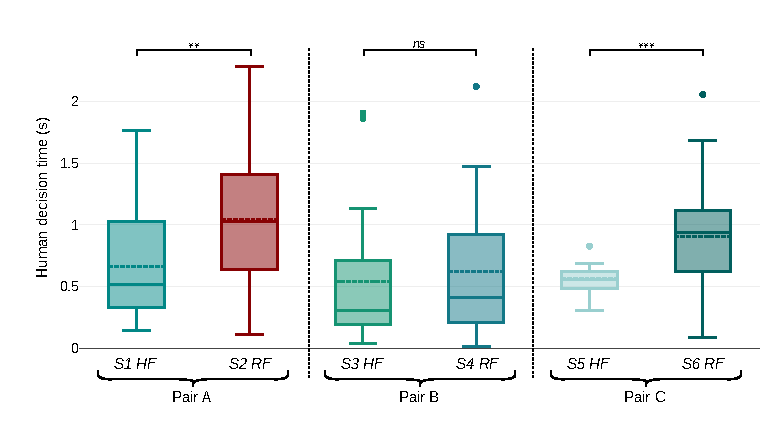
\includegraphics[width=\linewidth]{Chapter6/decision_time.pdf}
    \caption{Average human decision time in the six scenarios. This decision time tends to be lower when using HF than with RF.}
    \label{fig:decision_time}
\end{figure}

Considering the defined scenario pairs, the decision time with RF tends to be longer. However, this difference is statically significant only for pair C (S5-S6). This is expected because when the robot places the first pink bar the human gets confused and takes time to adapt to the situation. On the other hand, this is not reflected in S4 despite the similar confusing robot actions. Indeed, in S4 the robot ``steals'' cubes from the human reach which is confusing, but this prevents the human from acting and thus no decision time can be computed.  

I think the overall slower human decision time in the RF scenarios is due to the fact that the human acts after the robot. This way, the human has to pay attention to the scene and to the robot action/intentions, which is longer than only looking at the scene like in HF scenarios.   

Overall the decision time of the human is an average of about $0.72s$.


\subsubsection*{Agent actions' duration}

\begin{figure}[h]
    \center
    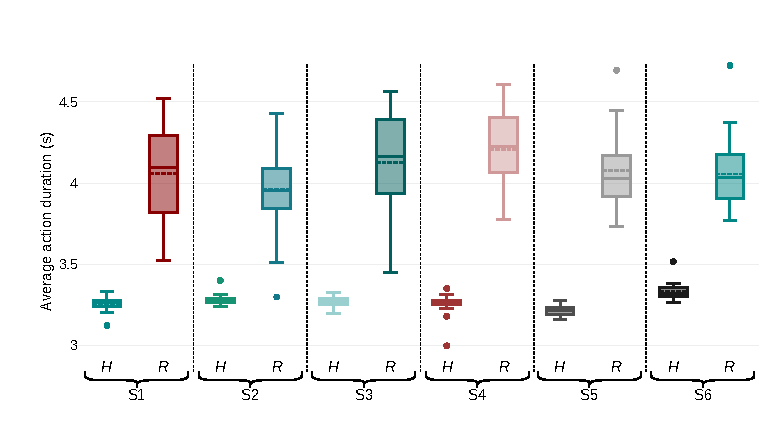
\includegraphics[width=\linewidth]{Chapter6/action_duration.pdf}
    \caption{Average action duration of the human and robot agents over the 6 scenarios, with standard deviations. Compared to the human action durations, the robot ones tend to be longer and have various durations.}
    \label{fig:action_durations}
\end{figure}

As depicted in fig.~\ref{fig:action_durations}, the human actions are in average significantly faster than the robot ones. In addition, the robot action durations tend to fluctuate more than the human one. This can be explained by the difference in motion execution between the avatar and the robot. The human has a simplified motion planner that simply moves the hand at a constant speed and in straight lines to the cubes or the stack. However, the robot uses a real motion planner to move its arm which is longer than the human motions. The motion planning process doesn't always found the same solutions, nor in the same amount of time. Meaning that both the motion planning duration and the motion execution duration can fluctuate. Here only the motion execution duration is considered in this metric. Note that to avoid having too much difference between the human and robot action durations, collisions with the dynamic objects are not considered in the robot motion planner, nor the objects' orientation. Hence, the robot can pick or place cubes from any angle and pass through the other cubes. When placing a cube its orientation is corrected. Collisions with the table where kept preventing the robot from picking cubes from below.  

Overall scenarios and steps, mean $=3.27s$ the maximum human action duration is $4.63s$ and the minimum is $2.55s$. For the robot, mean=$4.09s$, the maximum action duration is $9.09$ and the minimum duration is $1.46$.

\subsection{From questionnaires}

This section is focused on providing the results obtained by analyzing the answers to the questionnaires filled by the participants after each scenario.

To help the reader understand the following plots we list here the items of the questionnaire from the table~\ref{tab:questionnaire_answers} with their associated numeric ID in table~\ref{tab:items_id}. These IDs will be used in many plots in the x-axis to analyze the questionnaire's answers.

\begin{table}[h]
    \center
    \begin{tabular}{|cl|cl|cl|cl|}
    \hline
    \multicolumn{2}{|c|}{\textbf{Robot perception}} & \multicolumn{2}{c|}{\textbf{Interaction}} & \multicolumn{2}{c|}{\textbf{Collaboration}} & \multicolumn{2}{c|}{\textbf{Acting}} \\ \hline
    1                 & Responsive                  & 4                & Positive               & 7                & Adaptive                 & 10          & Appropriate            \\ \hline
    2                 & Competent                   & 5                & Simple                 & 8                & Useful                   & 11          & Accommodating          \\ \hline
    3                 & Intelligent                 & 6                & Clear                  & 9                & Efficient                & 12          & Predictable            \\ \hline
    \end{tabular}
    \caption{Questionnaire items with their associated IDs.}
    \label{tab:items_id}
    \end{table}


\subsubsection{Overall analysis}

We start by commenting overall questionnaire's results using some relevant average values and standard deviations before having a deeper statistical analysis in the next subsection.

\begin{figure}[h]
    \center
    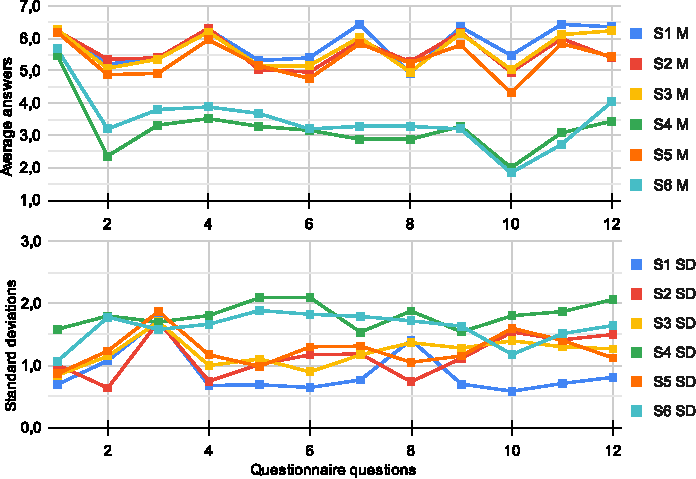
\includegraphics[width=\linewidth]{Chapter6/scenario_answers.pdf}
    \caption{W.r.t. each scenario, average answers (M, top) and standard deviations (SD, bottom) obtained for each question of the questionnaire.}
    \label{fig:scenario_answers}
\end{figure}

Figure~\ref{fig:scenario_answers} depicts the answers obtained for each question of the questionnaire w.r.t. each scenario. This figure provides a very visual overall summary of the study. On the top part, for each of the 12 questions on the x-axis, the average answers obtained are plotted for each scenario, 7 being the maximal or best value and 1 being the minimal or worst value. 
We can see that four scenarios obtained quite similar high answers whereas scenarios S4 and S6 have noticeably worse answers. Those scenarios are the Robot-First scenarios of pairs B and C where the robot has an erroneous, and even adversarial, estimation of human preferences. 
Note that question 1 (Q1) which evaluates the reactivity of the robot is the only question which answers are relatively high in every scenario.
Considering the answers to all other questions than Q1, S4 and S6 seem to deviate significantly from the other scenarios which can be analyzed as follows.
First, it means that with a correct estimation both HF and RF regimes are roughly perceived similarly. 
Second, an erroneous estimation doesn't seem to induce lower answers, and thus, despite the wrong estimation the robot in S3 and S5 is roughly perceived similarly to the one in S1 with a correct estimation.
On the other hand, when using RF, an erroneous estimation seems to have a significant detrimental impact on how the robot is perceived by the participants.
All these preliminary conclusions will be confirmed in the statistical analysis below.

It is also worth commenting on the standard deviations obtained, depicted in the bottom part of figure~\ref{fig:scenario_answers}. The standard deviations depend a lot on the scenarios and go from $0.6$ up to $2.1$. There are two noticeable facts to comment on.
First, question 3 evaluating how intelligent the robot is perceived is the only question with a relatively high SD for every scenario. Participants had various definitions of ``intelligence'' which led to a wide range of answers. Some participants evaluated the intelligence of the robot on its choices of actions, and thus, fluctuated depending on the scenario. Some others evaluated the intelligence of the robot on other criteria independent of the robot's decisions. Thus, they would rather indicate that the robot was always intelligent (or not) over all scenarios.
Additionally, we can see that the SD of S4 and S6 seem to be higher than the other scenarios.

\begin{figure}[h]
    \center
    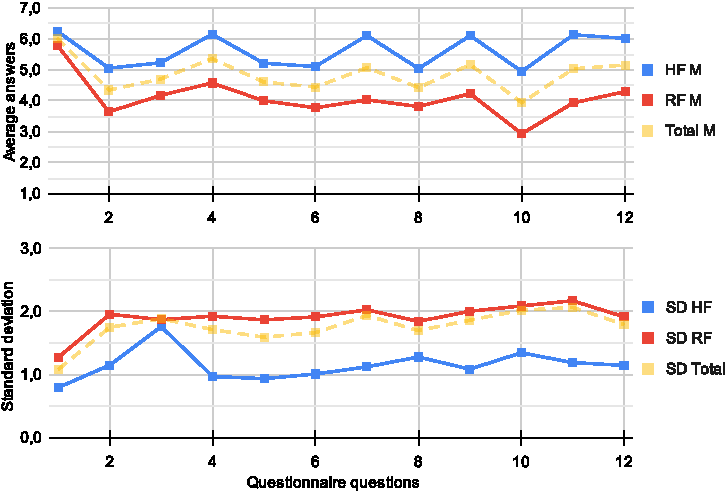
\includegraphics[width=\linewidth]{Chapter6/regime_answers.pdf}
    \caption{W.r.t. each regime of execution, average answers (M, top) and standard deviations (SD, bottom) obtained for each question of the questionnaire.}
    \label{fig:regime_answers}
\end{figure}

In contrast with the previous figure, Figure~\ref{fig:regime_answers} shows the answers obtained for each question w.r.t. to each execution regime. Indeed, the HF average answers and standard deviations, shown in blue, correspond to the union of the scenario's answers using the Human-First regime, i.e., $S1 \cup S3 \cup S5$. Similarly, the RF values, shown in red, correspond to $S2 \cup S4 \cup S6$ where the Robot-First regime is used. Additionally, the results for all scenarios combined are shown in light yellow. The results shown here can be deduced from the previous figure since we already commented on all scenarios. Yet, this new figure highlights more visually the difference between the HF and RF regimes. 

The first noticeable fact is that when using the HF regime the average answers for each question are better than when using the RF regime. Again, the only question where the answers are roughly the same regardless of the regime is when questioning the reactivity of the robot. HF's average answers are relatively high for all questions which indicates that the collaborations with HF seem to be appreciated. On the other hand, RF's answers are average (around 4) which indicates that collaborating with RF seems to be less appreciated.

Concerning the standard deviations, it is also noticeable that the answers concerning the RF regime have higher SD. This indicates that there was a wider range of answers from the participants when collaborating with the RF regime. This means that participants tend to be less certain about their answers when evaluating RF than with HF. This can be expected because when facing the HF regime the collaboration is overall quite positive, thus, participants concentrated their answers on the higher part of the scales. However, the frustrating robot actions due to the RF regime degraded the collaboration and participants had to evaluate how bad this degradation is. Some participants were more emotionally affected than others by the robot's actions, hence, it led to a wide range of answers.
Another interesting fact is that regardless of the regime, question 3 has a high standard deviation. This question evaluates the \textit{intelligence} of the robot. Participants had various definitions of intelligence which is reflected in this high SD. Indeed, some participants evaluated the robot as unintelligent because of its nature and thus regardless of its actions or the scenario. Others perceived less intelligence when the robot performed frustrating actions. 
Also, we can see that the SD regarding the reactivity of the robot is quite close and low for both regimes. This is a consequence of the very high average values regarding Q1 for both regimes.   

Eventually, I would like to insist on the average answers concerning the RF regime. Even if these answers are mediocre, it is important to note that they are not very low. In comparison, consider another robot behaving completely erratically. This robot would randomly pick and place cubes around itself. As a consequence, the robot would neither help the human nor solve the task, on the contrary, it might only disturb the human trying to achieve the task. The robot could make the task impossible to solve for the human by picking a relevant cube and never placing it, or by removing already well-placed cubes from the stack. Here, during one step, the RF regime forces the human to comply with the robot's decisions which can be frustrating. However, the robot takes into account the human action anyway and adapts accordingly its actions for the next step. This is thanks to our planning approach, common to both regimes, which explores every possible human action to generate the robot policy. Thus, we can say that our planning approach seems to benefit the collaboration and interaction between the human and the robot.

\subsubsection{ANOVA Analysis}

So far, we only conducted a preliminary analysis of the questionnaire's answers using only the average values and standard deviations. Now, a statistical analysis must be conducted to confirm the preliminary comments of the previous subsection. For each question, and thus each item of the questionnaire, we performed an analysis of the variance with repeated measures. Each analysis led to p-values $<=0.001$ indicating that there is a significant difference between the 6 scenarios. To evaluate the strength of this significant difference the effect size Eta squared $\eta^2$ has been calculated where the limits are $.01$ (small effect), $.06$ (medium effect), and $.14$ (large effect). However, ANOVA tests can only indicate if there is a significant difference between N-samples, but it is only of interest to identify between which exact group that difference exists.  In the Bonferroni post-hoc test in a repeated measures ANOVA, multiple t-tests are calculated for dependent samples. However, the problem with multiple testing is that the so-called alpha error (the false rejection of the null hypothesis) increases with the number of tests. To counteract this, the Bonferroni post-hoc test calculates the obtained p-values times the number of tests. The obtained p-values indicate in a pairwise manner between which samples the significant difference exists. The results from the ANOVA and Bonferroni post-hoc test are shown in table~\ref{tab:questionnaire_answers}.

\begin{sidewaystable}
    \center
        \begin{tabular}{c|cc|ccccccccccccccc|}
        \cline{2-18}
        \multicolumn{1}{l|}{}                        & \multicolumn{2}{c|}{\textbf{ANOVA}}                                 & \multicolumn{15}{c|}{\textbf{Bonferroni Post hoc tests}}                                                                                                                                                                                                                                                                                                                                                                                                                                                                                                                                                                        \\ \cline{2-18} 
        \multicolumn{1}{l|}{}                        & \multicolumn{1}{c|}{p}            & $\eta^2$               & \multicolumn{1}{c|}{1-2}         & \multicolumn{1}{c|}{1-3}         & \multicolumn{1}{c|}{\textbf{1-4}}          & \multicolumn{1}{c|}{1-5}                  & \multicolumn{1}{c|}{\textbf{1-6}}          & \multicolumn{1}{c|}{2-3}         & \multicolumn{1}{c|}{\textbf{2-4}}          & \multicolumn{1}{c|}{2-5}         & \multicolumn{1}{c|}{\textbf{2-6}}          & \multicolumn{1}{c|}{\textbf{3-4}}          & \multicolumn{1}{c|}{3-5}                 & \multicolumn{1}{c|}{\textbf{3-6}}          & \multicolumn{1}{c|}{\textbf{4-5}}          & \multicolumn{1}{c|}{4-6}         & \textbf{5-6}          \\ \hline
        \multicolumn{1}{|c|}{Responsive}             & \multicolumn{1}{c|}{\textit{***}} & \textit{0.16}          & \multicolumn{1}{c|}{\textit{ns}} & \multicolumn{1}{c|}{\textit{ns}} & \multicolumn{1}{c|}{\textit{ns}}           & \multicolumn{1}{c|}{\textit{ns}}          & \multicolumn{1}{c|}{\textit{ns}}           & \multicolumn{1}{c|}{\textit{ns}} & \multicolumn{1}{c|}{\textit{ns}}           & \multicolumn{1}{c|}{\textit{ns}} & \multicolumn{1}{c|}{\textit{ns}}           & \multicolumn{1}{c|}{\textit{ns}}           & \multicolumn{1}{c|}{\textit{ns}}         & \multicolumn{1}{c|}{\textit{ns}}           & \multicolumn{1}{c|}{\textit{ns}}           & \multicolumn{1}{c|}{\textit{ns}} & \textit{ns}           \\ \hline
        \multicolumn{1}{|c|}{Competent}              & \multicolumn{1}{c|}{\textit{***}} & \textit{0.49}          & \multicolumn{1}{c|}{\textit{ns}} & \multicolumn{1}{c|}{\textit{ns}} & \multicolumn{1}{c|}{\textit{\textbf{***}}} & \multicolumn{1}{c|}{\textit{ns}}          & \multicolumn{1}{c|}{\textit{\textbf{***}}} & \multicolumn{1}{c|}{\textit{ns}} & \multicolumn{1}{c|}{\textit{\textbf{***}}} & \multicolumn{1}{c|}{\textit{ns}} & \multicolumn{1}{c|}{\textit{\textbf{***}}} & \multicolumn{1}{c|}{\textit{\textbf{***}}} & \multicolumn{1}{c|}{\textit{ns}}         & \multicolumn{1}{c|}{\textit{\textbf{**}}}  & \multicolumn{1}{c|}{\textit{\textbf{***}}} & \multicolumn{1}{c|}{\textit{ns}} & \textit{\textbf{*}}   \\ \hline
        \multicolumn{1}{|c|}{Intelligent}            & \multicolumn{1}{c|}{\textit{***}} & \textit{0.33}          & \multicolumn{1}{c|}{\textit{ns}} & \multicolumn{1}{c|}{\textit{ns}} & \multicolumn{1}{c|}{\textit{\textbf{**}}}  & \multicolumn{1}{c|}{\textit{ns}}          & \multicolumn{1}{c|}{\textit{\textbf{*}}}   & \multicolumn{1}{c|}{\textit{ns}} & \multicolumn{1}{c|}{\textit{\textbf{**}}}  & \multicolumn{1}{c|}{\textit{ns}} & \multicolumn{1}{c|}{\textit{\textbf{**}}}  & \multicolumn{1}{c|}{\textit{\textbf{**}}}  & \multicolumn{1}{c|}{\textit{ns}}         & \multicolumn{1}{c|}{\textit{\textbf{***}}} & \multicolumn{1}{c|}{\textit{\textbf{*}}}   & \multicolumn{1}{c|}{\textit{ns}} & \textit{\textbf{*}}   \\ \hline
        \multicolumn{1}{|c|}{\textbf{Positive}}      & \multicolumn{1}{c|}{\textit{***}} & \textit{\textbf{0.65}} & \multicolumn{1}{c|}{\textit{ns}} & \multicolumn{1}{c|}{\textit{ns}} & \multicolumn{1}{c|}{\textit{\textbf{***}}} & \multicolumn{1}{c|}{\textit{ns}}          & \multicolumn{1}{c|}{\textit{\textbf{***}}} & \multicolumn{1}{c|}{\textit{ns}} & \multicolumn{1}{c|}{\textit{\textbf{***}}} & \multicolumn{1}{c|}{\textit{ns}} & \multicolumn{1}{c|}{\textit{\textbf{***}}} & \multicolumn{1}{c|}{\textit{\textbf{***}}} & \multicolumn{1}{c|}{\textit{ns}}         & \multicolumn{1}{c|}{\textit{\textbf{***}}} & \multicolumn{1}{c|}{\textit{\textbf{***}}} & \multicolumn{1}{c|}{\textit{ns}} & \textit{\textbf{***}} \\ \hline
        \multicolumn{1}{|c|}{Simple}                 & \multicolumn{1}{c|}{\textit{***}} & \textit{0.34}          & \multicolumn{1}{c|}{\textit{ns}} & \multicolumn{1}{c|}{\textit{ns}} & \multicolumn{1}{c|}{\textit{\textbf{**}}}  & \multicolumn{1}{c|}{\textit{ns}}          & \multicolumn{1}{c|}{\textit{\textbf{**}}}  & \multicolumn{1}{c|}{\textit{ns}} & \multicolumn{1}{c|}{\textit{\textbf{**}}}  & \multicolumn{1}{c|}{\textit{ns}} & \multicolumn{1}{c|}{\textit{ns}}           & \multicolumn{1}{c|}{\textit{\textbf{*}}}   & \multicolumn{1}{c|}{\textit{ns}}         & \multicolumn{1}{c|}{\textit{\textbf{*}}}   & \multicolumn{1}{c|}{\textit{\textbf{**}}}  & \multicolumn{1}{c|}{\textit{ns}} & \textit{\textbf{*}}   \\ \hline
        \multicolumn{1}{|c|}{Clear}                  & \multicolumn{1}{c|}{\textit{***}} & \textit{0.41}          & \multicolumn{1}{c|}{\textit{ns}} & \multicolumn{1}{c|}{\textit{ns}} & \multicolumn{1}{c|}{\textit{\textbf{***}}} & \multicolumn{1}{c|}{\textit{ns}}          & \multicolumn{1}{c|}{\textit{\textbf{***}}} & \multicolumn{1}{c|}{\textit{ns}} & \multicolumn{1}{c|}{\textit{\textbf{**}}}  & \multicolumn{1}{c|}{\textit{ns}} & \multicolumn{1}{c|}{\textit{\textbf{***}}} & \multicolumn{1}{c|}{\textit{\textbf{***}}} & \multicolumn{1}{c|}{\textit{ns}}         & \multicolumn{1}{c|}{\textit{\textbf{***}}} & \multicolumn{1}{c|}{\textit{\textbf{*}}}   & \multicolumn{1}{c|}{\textit{ns}} & \textit{\textbf{**}}  \\ \hline
        \multicolumn{1}{|c|}{\textbf{Adaptive}}      & \multicolumn{1}{c|}{\textit{***}} & \textit{\textbf{0.62}} & \multicolumn{1}{c|}{\textit{ns}} & \multicolumn{1}{c|}{\textit{ns}} & \multicolumn{1}{c|}{\textit{\textbf{***}}} & \multicolumn{1}{c|}{\textit{ns}}          & \multicolumn{1}{c|}{\textit{\textbf{***}}} & \multicolumn{1}{c|}{\textit{ns}} & \multicolumn{1}{c|}{\textit{\textbf{***}}} & \multicolumn{1}{c|}{\textit{ns}} & \multicolumn{1}{c|}{\textit{\textbf{***}}} & \multicolumn{1}{c|}{\textit{\textbf{***}}} & \multicolumn{1}{c|}{\textit{ns}}         & \multicolumn{1}{c|}{\textit{\textbf{***}}} & \multicolumn{1}{c|}{\textit{\textbf{***}}} & \multicolumn{1}{c|}{\textit{ns}} & \textit{\textbf{***}} \\ \hline
        \multicolumn{1}{|c|}{Useful}                 & \multicolumn{1}{c|}{\textit{***}} & \textit{0.43}          & \multicolumn{1}{c|}{\textit{ns}} & \multicolumn{1}{c|}{\textit{ns}} & \multicolumn{1}{c|}{\textit{\textbf{***}}} & \multicolumn{1}{c|}{\textit{ns}}          & \multicolumn{1}{c|}{\textit{\textbf{*}}}   & \multicolumn{1}{c|}{\textit{ns}} & \multicolumn{1}{c|}{\textit{\textbf{***}}} & \multicolumn{1}{c|}{\textit{ns}} & \multicolumn{1}{c|}{\textit{\textbf{***}}} & \multicolumn{1}{c|}{\textit{\textbf{***}}} & \multicolumn{1}{c|}{\textit{ns}}         & \multicolumn{1}{c|}{\textit{\textbf{**}}}  & \multicolumn{1}{c|}{\textit{\textbf{***}}} & \multicolumn{1}{c|}{\textit{ns}} & \textit{\textbf{***}} \\ \hline
        \multicolumn{1}{|c|}{\textbf{Efficient}}     & \multicolumn{1}{c|}{\textit{***}} & \textit{\textbf{0.62}} & \multicolumn{1}{c|}{\textit{ns}} & \multicolumn{1}{c|}{\textit{ns}} & \multicolumn{1}{c|}{\textit{\textbf{***}}} & \multicolumn{1}{c|}{\textit{ns}}          & \multicolumn{1}{c|}{\textit{\textbf{***}}} & \multicolumn{1}{c|}{\textit{ns}} & \multicolumn{1}{c|}{\textit{\textbf{***}}} & \multicolumn{1}{c|}{\textit{ns}} & \multicolumn{1}{c|}{\textit{\textbf{***}}} & \multicolumn{1}{c|}{\textit{\textbf{***}}} & \multicolumn{1}{c|}{\textit{ns}}         & \multicolumn{1}{c|}{\textit{\textbf{***}}} & \multicolumn{1}{c|}{\textit{\textbf{***}}} & \multicolumn{1}{c|}{\textit{ns}} & \textit{\textbf{***}} \\ \hline
        \multicolumn{1}{|c|}{\textbf{Appropriate}}   & \multicolumn{1}{c|}{\textit{***}} & \textit{\textbf{0.62}} & \multicolumn{1}{c|}{\textit{ns}} & \multicolumn{1}{c|}{\textit{ns}} & \multicolumn{1}{c|}{\textit{\textbf{***}}} & \multicolumn{1}{c|}{\textit{\textbf{**}}} & \multicolumn{1}{c|}{\textit{\textbf{***}}} & \multicolumn{1}{c|}{\textit{ns}} & \multicolumn{1}{c|}{\textit{\textbf{***}}} & \multicolumn{1}{c|}{\textit{ns}} & \multicolumn{1}{c|}{\textit{\textbf{***}}} & \multicolumn{1}{c|}{\textit{\textbf{***}}} & \multicolumn{1}{c|}{\textit{ns}}         & \multicolumn{1}{c|}{\textit{\textbf{***}}} & \multicolumn{1}{c|}{\textit{\textbf{***}}} & \multicolumn{1}{c|}{\textit{ns}} & \textit{\textbf{***}} \\ \hline
        \multicolumn{1}{|c|}{\textbf{Accommodating}} & \multicolumn{1}{c|}{\textit{***}} & \textit{\textbf{0.68}} & \multicolumn{1}{c|}{\textit{ns}} & \multicolumn{1}{c|}{\textit{ns}} & \multicolumn{1}{c|}{\textit{\textbf{***}}} & \multicolumn{1}{c|}{\textit{ns}}          & \multicolumn{1}{c|}{\textit{\textbf{***}}} & \multicolumn{1}{c|}{\textit{ns}} & \multicolumn{1}{c|}{\textit{\textbf{***}}} & \multicolumn{1}{c|}{\textit{ns}} & \multicolumn{1}{c|}{\textit{\textbf{***}}} & \multicolumn{1}{c|}{\textit{\textbf{***}}} & \multicolumn{1}{c|}{\textit{ns}}         & \multicolumn{1}{c|}{\textit{\textbf{***}}} & \multicolumn{1}{c|}{\textit{\textbf{***}}} & \multicolumn{1}{c|}{\textit{ns}} & \textit{\textbf{***}} \\ \hline
        \multicolumn{1}{|c|}{Predictable}            & \multicolumn{1}{c|}{\textit{***}} & \textit{0.45}          & \multicolumn{1}{c|}{\textit{ns}} & \multicolumn{1}{c|}{\textit{ns}} & \multicolumn{1}{c|}{\textit{\textbf{***}}} & \multicolumn{1}{c|}{\textit{\textbf{**}}} & \multicolumn{1}{c|}{\textit{\textbf{***}}} & \multicolumn{1}{c|}{\textit{ns}} & \multicolumn{1}{c|}{\textit{\textbf{*}}}   & \multicolumn{1}{c|}{\textit{ns}} & \multicolumn{1}{c|}{\textit{\textbf{*}}}   & \multicolumn{1}{c|}{\textit{\textbf{***}}} & \multicolumn{1}{c|}{\textit{\textbf{*}}} & \multicolumn{1}{c|}{\textit{\textbf{***}}} & \multicolumn{1}{c|}{\textit{\textbf{**}}}  & \multicolumn{1}{c|}{\textit{ns}} & \textit{\textbf{**}}  \\ \hline
        \end{tabular}
        \caption{Significant differences in the questionnaire answers between the different scenarios. For each item of the questionnaire are shown the overall p-value and $\eta^2$ (effect size) obtained after an ANOVA. Additionally, the p values obtained after conducting Bonferroni Post-hoc-Tests are shown to identify in a pair-wise manner which scenarios were significantly different from others. As depicted, scenarios 4 and 6 are distinguishable from the others and their evaluation are significantly different on all the measured aspect (expect reactivity).}
        \label{tab:questionnaire_answers}
\end{sidewaystable}

As suggested by the preliminary analysis, the Reactivity of the robot is the item with the lowest difference. The ANOVA indicates that answers regarding the reactivity are significantly different with a large effect over the 6 scenarios. However, compared to other items, the effect size $\eta^2$ is quite low indicating that this difference is less significant than for other items. Also, the Bonferroni post-hoc test wasn't able to identify where exactly the difference exists, which means again that this difference isn't very significant in the end. 

Besides reactivity, all other items have large significant differences according to the scenario which can be exploited using the Bonferroni post-hoc test. 
Indeed, the pairwise comparisons indicate the existence of major significant differences for every question in the following pairs: S1-S4, S1-S6, S2-S4, S2-S6, S3-S4, S3-S6, S4-S5, and S5-S6 (in bold in the table). Having in mind that S4 and S6 are the two scenarios using Robot-First with erroneous estimations, we can see that erroneous estimation with RF systematically leads to significant differences compared to all other scenarios using HF or RF with a correct estimation (S4-S1, S4-S2, S4-S3, S4-S5, and S6-S1, S6-S2, S6-S3, S6-S5). This is a clear indicator that the RF regime is very sensitive to the estimation of the human preferences and thus an erroneous estimation is significantly detrimental to the collaboration and the overall interaction. 

Only a few other significant differences exist and are in S1-S5 and S3-S5. Indeed, in S5, the robot's actions were perceived as more or less significantly less appropriate ($p=0.004$) and predictable ($p=0.004$) than in S1, slightly less predictable ($p=0.017$) than in S3. Indeed, in S5 the HF robot surprisingly picks up its pink bar while the human picks up its own whereas the human wants to place their bar to be freed from the task. Using HF allows the human to place their bar anyway, but the robot actions were therefore perceived as less predictable and appropriate than in S1 or S3. 
We can also notice that despite S3 having an erroneous estimation in contrast to S1, there is no significant difference in answers for each question between S1 and S3. 
This indicates that using the HF regime allows the robot to be way more robust to erroneous estimation than RF. However, the few existing significant differences among the HF scenarios indicate that an erroneous estimation is still noticeable and can still have a detrimental influence. Thus, the robot cannot fully rely on being reactive and compliant to human actions. Estimating the human preferences accurately to plan appropriately the robot's actions is mandatory for optimal collaboration.

Looking at the eta squared $\eta^2$ of every question, one can notice that we can group the items into 4 groups. 
% First, the Reactivity item is alone with the lowest effect size ($\eta^2=0.16$). This group doesn't really help to distinguish the regimes. 
% Secondly, with an effect size of around $\eta^2 \simeq 0.33$, we can state that when using RF the robot was perceived as slightly less intelligent and the interaction as slightly less simple than when using HF. 
% Then, with an effect size of around $\eta^2 \simeq 0.45$, we can state that when using RF the robot was perceived as moderately less competent, the interaction as moderately less clear, the collaboration as moderately less useful, and the robot actions as moderately less predictable. 
% Eventually, with an effect size of around $\eta^2 \simeq 0.64$, when using the RF regime the interaction was perceived as significantly less positive, the collaboration as significantly less adaptive and efficient, and the robot actions as significantly less appropriate and less accommodation. 
% Since the five items from the last group are the ones with the highest effect size, they can be seen as the main characteristics differentiating the HF from the RF regimes and thus are highlighted in the table.
\begin{enumerate}
    \item $\eta^2=0.16$: First, the Reactivity item is alone with the lowest effect size. This group doesn't help to distinguish the regimes. 
    \item $\eta^2 \simeq 0.33$: Secondly, we can state that when using RF the robot was perceived as slightly less intelligent and the interaction as slightly less simple than when using HF. 
    \item $\eta^2 \simeq 0.45$: Then, due to the moderate effect size, we can state that when using RF the robot was perceived as moderately less competent, the interaction as moderately less clear, the collaboration as moderately less useful, and the robot actions as moderately less predictable. 
    \item $\eta^2 \simeq 0.64$: Eventually, with a high effect size, when using the RF regime the interaction was perceived as significantly less positive, the collaboration as significantly less adaptive and efficient, and the robot actions as significantly less appropriate and less accommodation. Since the five items from the last group are the ones with the highest effect size, they can be seen as the main characteristics differentiating the HF from the RF regimes and thus are highlighted in the table.
\end{enumerate}

% ***

% Except reactive, all Q significantly vary according to scenarios

% S4 and S6 are significantly different from others

% with effect size talk about Q that are most diff [~0.6-0.7] (Positive, Adaptive, Efficient, Appropriate, Accommodating), 

% medium diff [~0.4-0.5] (Competent, Clear, Useful, Predictable), 

% low diff [~0.3] (Intelligent, Simple) 

% and lowest [0.16] (Reactive)

% Talk about the few other diff (1-5, )

% *****

% Some questions have large standard deviations, such as about the perceived ``Intelligence'', but often only on specific scenarios.

% The ``Reactive'' answers are overall the same, whatever execution regime and scenario. 
% Overall, based on an ANalysis Of the VAriance with repeated measures (ANOVA), all other answers than ``Reactive'' vary significantly. Post-tests show that the main differences come from scenarios S4 and S6. Those two scenarios correspond to ones where the robot has an incorrect estimation of the human preferences and is following the \textit{Robot-First} execution regime. This indicates that all HF behaviors are perceived similarly despite the erroneous estimation of the robot. It also indicates that the RF scenario with correct estimation is positively perceived, but an erroneous estimation has a significant impact on the answers when using RF.  

% Except for the ``Reactive'' aspect, answers about RF have a larger standard deviation. Thus, participants tend to be more indecisive regarding RF than HF.

% About ``Reactive''. A Bonferroni Post hoc test was used to compare the groups in pairs to find out which was significantly different.
% Despite the significant difference in the ANOVA, no pairwise group comparison was significant in the Bonferroni Post hoc test; all p values were greater than 0,05. 

% S4 and S6 received significantly worse answers than the other scenarios. It is interesting to notice that in a pair-wise manner, all other scenarios 

% We notice very few significant differences on HF only.

% In table \ref{tab:questionnaire_answers} there almost only significant differences in pairs involving S4 and S6. The only few other differences are the following. 
% S1 is significantly more appropriate than S5. And S5 is significantly less predictable than S1 and S3

% \begin{figure}[h]
%     \centering
%     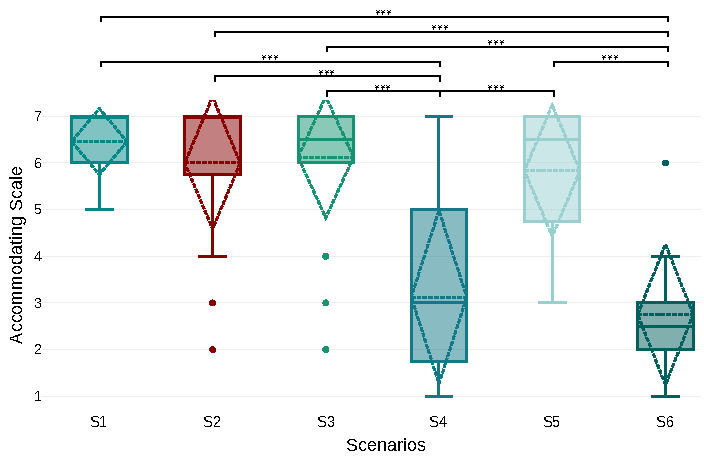
\includegraphics[width=\linewidth]{Chapter6/signif_accommo.pdf}
%     \caption{Accommodating Interaction Scale with ANOVA + Post-hoc-Tests}
%     \label{fig:accommodating_scale_anova}
% \end{figure}

\subsection{From comments}

At the end of the experiment, every participant was asked two questions gathering their general impressions. First, they were asked to comment on the overall experiment and robot interaction they just had. Secondly, participants were asked to indicate which scenario they preferred the most and the least. 

Participants' comments concern several aspects of the experiment and are worth discussing. Overall, the comments confirm the outcome of the statistical analysis, and they also provide some feedback about the overall experiment protocol and conditions, especially regarding the simulator itself. The comments are discussed per categories below. 

\textbf{TODO: Try to add more argumentation and links to previous results, be less descriptive...}

\subsubsection{Simulation}
First, most of the participants found the experiment and the simulation as a good experience. They felt committed and active during the different scenarios. 
The simulation has been described several times as clear, simple, pleasant, intuitive, captivating, and funny. 
Some participants mentioned that it was like a video game and enjoyed it. 
These comments suggest that collaborating with a simulated robot has been appreciated, and they raise the question if the participant had felt the same way in an experiment with a real robot. 

\subsubsection{Display}
Some participants think that the simulation display had too much information (goal + scene + text prompt), and a few had trouble reading the text prompt. Yet, the robot can be seen well. Indeed, the text prompts could be a bit fast and written white on black, which can be disturbing when not used to. However, I believe this didn't affect much the executions, maybe slightly the decision times. 

\subsubsection{General}
A few participants would have appreciated the robot giving instructions and guidance regarding the actions to perform. This is linked to another comment saying that using the Robot-Fist regime with correct estimation felt better because makes the task simpler. If the human trusts the robot, it can be appreciated to let the robot compute the optimal plan and just follow the robot's instructions, lowering the cognitive load of the human. Indeed, some participants consider that they made mistakes and that they could have acted in a better way in some scenarios. 

\subsubsection{Steps}
The step synchronization wasn't appreciated by everyone. Some participants found this kind of synchronization useful as it structured the collaboration. However, many others found this a bit confusing at first and frustrating because they had to wait for the robot's actions to be done before being able to act again.

\subsubsection{Task}
The task was found clear and quite simple. One participant said that they felt significant emotions such as satisfaction and frustration and that if the task was less abstract and more real, these emotions would have been enhanced. Moreover, another participant said that in such simple tasks, humans tend to think they know better how to solve the task than the robot. Thus, the robot should follow human decisions in such cases, with a hierarchy relation. A few participants also mentioned that performing the last action, i.e. placing the last cube, is very satisfying. These people liked the robot adapting to allow them to do so. 
The fact that both agents must perform actions to solve the task makes the collaboration relevant and useful. 

\subsubsection{Action}
Many participants said that not being able to pick cubes in advance isn't natural and, at first, it is confusing, frustrating, and a bit complicated. Yet, they also said that they got used to it quite fast. One also said that they felt obliged to act at every step. Indeed, a majority of the participants were signaling their passivity to the robot even when they were not able to act. 
About the movements, one participant stated that the actions were stiff and rigid, in contrast to being able to drag and drop the cubes thanks to the physics simulation. Additionally, the lack of collision with the cubes felt a bit unrealistic but not very confusing.
On the other hand, another participant said that the robot's movements seem real. This is probably due to the fact we used an online motion planner to move the robot arm, thus, the movements were not always optimal.

\subsubsection{Objective}
A few participants said that the objective of "trying to be free early" is a bit frustrating since they would like to keep acting, even if not necessary. It was hard for them to consider this objective as their personal preference, and thus, to act accordingly. 
Additionally, one participant mentioned that Scenario 5 creates double satisfaction: being free early (preferences) and the task is fulfilled.

\subsubsection{Regimes}
One participant said that they didn't see much difference between the two execution regimes HF and RF. The same participant couldn't indicate which scenario they preferred at the end. Moreover, some participants also indicated that the difference between HF and RF was unclear at first. However, once used to the task and the scenarios, the difference becomes clearer and before the end of the experiment, most of the participants had a clear idea of each regime, and even apprehended the RF one.

\subsubsection{Being in control}
Participants indicated that when using HF they felt in control, free to decide which action they performed, and that the robot was adapting to their decisions and actions, which was appreciated. In contrast, when using RF, participants didn't feel in control and were forced to adapt to the robot's decisions. Even when the robot's decisions are good, the lack of control is uncomfortable. One participant stated that they disliked when the robot took initiative because the robot could be wrong. 

\subsubsection{Human-First (HF) regime}
Most of the participants enjoyed the HF regime and stated that they were able to fulfill their objective with it. Some comments qualify the HF regime as slower than RF and sometimes inconsistent. The latter is mostly referring to the robot picking up the pink bar in S5. However, especially when used to it, HF has been qualified as smooth, efficient, interesting, predictable, and less frustrating than RF. Several participants mentioned that they enjoyed being able to predict the robot's behavior, proving that having predictable behavior is crucial for a seamless collaboration. It has been mentioned that HF makes less wrong choices than RF.
Moreover, some participants said that compared to the RF regime with a correct estimation HF is less efficient, however, in pairs B and C HF is more efficient than RF.

\subsubsection{Robot-First (RF) regime}
RF, bad, not in control, bad choices: having to drop bar + using common resources first

Every participant had an overall negative opinion regarding the RF regime. The latter has been qualified as very frustrating, confusing, constraining, unpredictable, inefficient, and even adversarial. A significant number of participants stated that to finish the task quickly RF could be great, fast, efficient, and less cognitively demanding, despite the lack of control. Also, a few participants noticed that even if during a specific step the human is forced to comply with the robot's actions, in the next step the robot takes into account the human action and adapts its behavior. 
However, it has been said that RF doesn't consider the human's objective or preferences. Participants really disliked when the robot forced them to drop a cube back on the table (pink bar in S6) and when the robot picked cubes in the middle zone instead of its own zone. The latter was perceived as the robot stealing the cubes from the human.
Due to those frustrating robot actions, the RF regime was putting the participants in an adversarial setup and the robots were explicitly qualified as ``enemies''. Some participants said that they were more focused on preventing the robot's mistakes than on the actual task.


\section{Discussion}

\textbf{TODO: to develop}

There are several elements to discuss in this study, including several participants' comments.

\begin{itemize}
    \item simulation to real life ? what would it take ? different results ? One in between solution is using VR. Requires flexible execution scheme like described in limitations in chapter \ref{chap:5}.
    \item Simu not realistic enough (pass trough cubes, no orientation, etc..): since focused on decisions, was enough but we could have done better. 
    \item Text prompt: Which info to prompt ? when ? and how (sometimes hard to read). maybe vocal would have been better ? Here no specific study has been conducted, we simply show to the participants some inner state of the robot (waiting for human, acting, identifying human action, ...)
    \item A different task ? only manipulation ? no navigation ?  Here the task carefully design to not be too long and still be significantly influenced by pairs of pref-esti
    \item Using an additional baseline with an erratic robot could have helped showing RF not so bad. 
\end{itemize}

\section{Conclusion}

% Our purpose was to validate thanks to this study both the overall planning approach as well as the model of execution Human-First which is key to our approach. 

% After statistically analyzing the execution log data as objective metrics, and the questionnaire answers and participants' comments as subjective metrics, we can confidently state that this study successfully validates both our planning approach and our model of execution. 

% Indeed, we have solid proof that the HF regime has been preferred by the participants because of the control it gives to the human. The robot is perceived as accommodating, adaptive, and acting appropriately while being predictable. HF also helps to better satisfy the human inner preferences which makes it more robust to erroneous estimations and thus more enjoyable. 
% On the other hand, we also show how the RF regime can be appreciated a lot when estimating correctly human preferences, but we also show how erroneous estimations are strongly detrimental to collaboration and interaction when using the RF regime. 
% Hence, the Human-First regime is preferred and allows for achieving smooth, efficient, and positive collaborations.
% Yet, we also show that even when using the Robot-First regime the robot is able to always solve the task with the human, thus, it is always found useful. It also still adapts to human actions in the next step thanks to our policy format. This means that our planning approach is still efficient and appropriate for this context. 

% ****

\textbf{TODO: be more specific which conclusion come from which data? preferences satisfaction from log, adjectives from questionnaire, from comments ? confirmation + discussion materials.}

Thanks to this study, we aimed to validate the overall planning approach and the model of execution Human-First, which is critical to our approach. 

After statistically analyzing the execution log data as objective metrics and the questionnaire answers and participants' comments as subjective metrics, we can confidently state that this study successfully validates both our planning approach and our model of execution. 

Indeed, we have solid proof that the  HF regime gives humans control over the execution, which was significantly appreciated. The participants perceived the robot as accommodating, adaptive, and acting appropriately while being predictable. HF also helps to satisfy better human inner preferences, which makes it more robust to erroneous estimations and thus more enjoyable. 
On the other hand, we show how the RF regime can be greatly appreciated when estimating human preferences correctly. However, we demonstrate how erroneous estimations strongly harm collaboration and interaction using the RF regime. 
Hence, the Human-First regime is preferred and allows for achieving smooth, efficient, and positive collaborations.
Nevertheless, thanks to our planning approach, we also show that the RF regime always solves the task with humans, and thus, it is always helpful. Additionally, it also always adapts to human action in the next step. 


\part{Social Navigating Agents Simulation} \label{part:2}
\cleardoublepage

\ifdefined\included
\else
\setcounter{chapter}{6} %% Numéro du chapitre précédent ;)
\dominitoc
\faketableofcontents
\fi

\chapter{Challenging Robot Navigation Systems by Simulating Intelligent Human: InHuS}
\chaptermark{Intelligent Human Simulation: InHuS}
\label{chap:7}
\minitoc

\chapabstract{This chapter describes the InHuS system, addressing decision-making in navigation and challenging robot navigation schemes. This chapter also compares two robot navigation systems using InHuS, proving that our approach effectively challenges robot schemes and allows measuring and comparing human-aware navigation properties.}

\section{Introduction}


Significant efforts are being dedicated today toward the development of robots that interact, assist, or work side-by-side with humans. However, people working in the field of \acrfull{hri} face constraining issues while testing and evaluating their systems. 
Apart from being mandatory to validate mature systems, experimenting using real humans and robots is burdensome: they are slow, hardly repeatable, expensive, etc. Moreover, the system needs to be run extensively for debugging and tuning before it reaches maturity. Doing so with real-life experiments is generally a long and tiresome process where colleagues in the lab and volunteers spend unproductive hours, if not days, interacting with a robot running a system under debugging. Moreover, such methods require exclusive physical access to the robot and a place to run the tests.

Simulations are well suited for such tasks as they allow working without a real robot or a physical space. Further, they allow multiple tests to run simultaneously and with a time factor greater than in real life. The simulated test environment can be changed very quickly compared to real-life tests. However, simulating realistic human behaviors and interactions is challenging, which could make simulations unreliable. Consequently, \acrshort{hri} researchers face some difficulties such as: ``How to test repeatedly and intensively their systems even when they are not sufficiently robust?'' and ``How to challenge their systems in a large variety of environments and situations?''. Therefore, there is a need for an ``intelligent artificial human'' that would help challenge the robot's interactive and decision-making abilities. 

\subsection{Human Simulations in Human-Aware Robot Navigation}

Being a part of \acrshort{hri}, the field of human-aware social robot navigation inherits all these limitations. One way to simulate an intelligent avatar in this field is to manually control the human avatar in real-time \cite{echeverria_simulating_2012}. 
This can be done using a variety of devices like a gaming controller, keyboard, or motion capture. Such approaches require a real human operator only focused on controlling the avatar, bringing back some already-mentioned limitations like human fatigue. On the other hand, autonomous human avatars seem to offer an adequate solution to this, but they often lack intelligence and rationality. 

Most of the current autonomous avatars available are either scripted or reactive. A scripted avatar executes a series of predefined actions, like following a fixed path, without being reactive to its environment, which limits interactions. Reactive agents use models like social force \cite{helbing1995social} or optimal reciprocal collision avoidance (ORCA) \cite{van2011reciprocal}. These highly scalable systems can simulate groups or even crowds of numerous agents. MengeROS \cite{aroor_mengeros_2018} and PedSim\_ROS\footnote{https://github.com/srl-freiburg/pedsim\_ros} are some examples. Despite their number, the generated agents usually fail in intricate social scenarios. Some recent works like VirtualHome~\cite{puig_virtualhome_2018} and SEAN~\cite{Tsoi_2020_HAI,tsoi2022sean} discuss simulating human agents to challenge robot systems, but the navigation of the agents in these systems is still based on reactive-only models. 
The work presented in~\cite{social_igibson} proposes a learning-based method to generate more realistic pedestrian navigation. This ongoing work shows an interesting navigation behavior like waiting and letting the other agent pass embedded in iGibson~\cite{shenigibson} simulator. However, this work is more focused on motion generation than decision-making to solve conflicts. 

We propose the \acrfull{inhus} System to contribute to the lack of intelligent and rational human agents with conflict-resolution skills to challenge the human-aware robot navigation systems. Our contribution includes 1) an intelligent human agent controller, 2) a high-level interface to control the simulated agents, and 3) a \acrfull{gui} to plot execution data and metrics for evaluating the interaction. Such a system could help people working in the field of human-aware robot navigation to test and debug their schemes. Our system is designed to run, analyze, and evaluate repeatable and long navigation scenarios involving a robot and an autonomous reactive and rational avatar. This work focuses on intricate and narrow scenarios where, in addition to being reactive, rational decisions should be taken in order to solve the conflicts occurring. Note that our contribution is focused on navigation decision-making and not the motion generation part. Throughout this paper, we use the term `rational' in a meaning close to Goal Reasoning~\cite{vattam_breadth_nodate,abbass_goal_2018}, i.e., the ability of autonomous agents that can dynamically reason about and adjust their goals. It enables the agents to adapt intelligently to changing conditions and unexpected events, allowing them to address a wide variety of complex situations.


\section{Architecture Description}
 
\begin{figure}[ht]
    \centering
    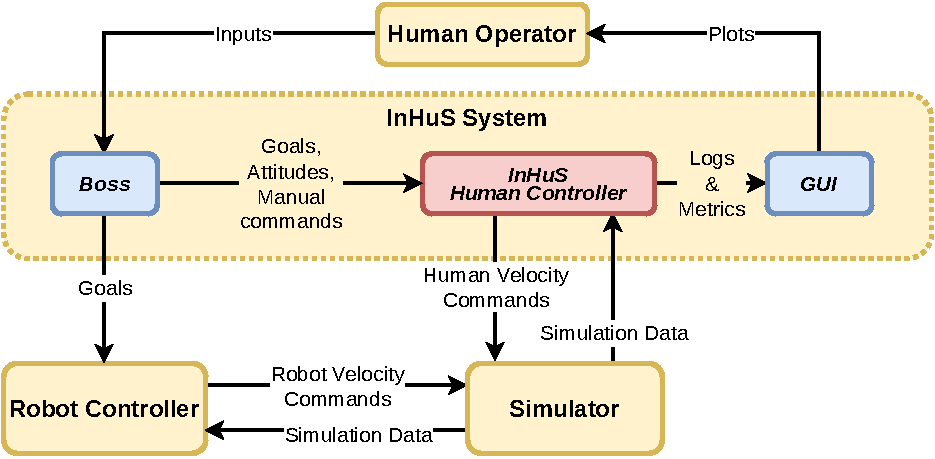
\includegraphics[width=0.7\linewidth]{Chapter7/Inhus.drawio.pdf}
    \caption{
    The InHuS System interacts with three external systems: the simulator, the robot controller, and a human operator. Our system is separated into three parts: the Boss high-level interface gathering inputs from the human operator, InHuS which is the actual human controller, and a \acrshort{gui} to plot the metrics and other data produced.
    }
    \label{fig:overview_inhus}
    \vspace{-0.8cm}
\end{figure}

The InHuS System%
\footnote{https://github.com/AnthonyFavier/InHuS\_Social\_Navigation}
works along with a human operator, a chosen simulator, and the challenged robot controller as depicted in Fig~\ref{fig:overview_inhus}. The system is mainly implemented using \acrshort{ros}. The InHuS  System is three-sided. First, the system comes with a high-level interface called Boss that helps to manage the simulated agents. Secondly, the main part is the intelligent human avatar controller itself, called InHuS.
Finally, a \acrshort{gui} provides an interactive visualization of the data and metrics computed by InHuS during execution that can help to evaluate interactions. Below, we present some details for each component.


\subsection{Boss}
For the human operator to easily control the simulated agents and run repeatable scenarios, we provide a simple graphical user interface component called Boss. Predefined or manually entered goals can be sent to the human, the robot, or both. Goals are by default considered as ``Pose goals'' that only require one navigation action to be achieved. However, the human agent (only) can handle ``Compound goals'' that need a specified sequence of navigation and waiting for actions to be achieved. This type of compound goal is useful to emulate more complex activities. For example, ``Make coffee'' could be described as a sequence of three actions: nav(coffeeMachine), wait(15$s$), nav(myOffice).

The Boss allows defining scenarios with start positions and goals for each agent to repeatedly generate the same situation. 
Running a scenario consists of first sending each agent to their respective starting position. Then, the corresponding goals are sent to the human and the robot.
A delay can be specified while starting the scenario to delay either the robot's or the human's goal. This is very useful to adjust the timing of a specific situation or conflict. The Boss can also put an agent in ``endless'' mode, where the agent continuously gets a new goal from a given list after completing one. 

Each navigation action can specify a radius for the ``Pose goal'', within which a new ``Pose goal'' is randomly sampled. This mechanism adds randomness to the execution and diversifies the situations encountered, especially in the ``endless'' mode. Setting the radius to zero disables the randomization and selects the given goal.

All the goals, scenarios, and endless goal sequences are defined using an XML format. Hence, defining new goals or scenarios is straightforward. There is an XML goal file associated with each map/environment. Thus, it is easy to switch between environments since the corresponding goal file is automatically loaded.


\subsection{InHuS}

\begin{figure}[b]
    \centering
    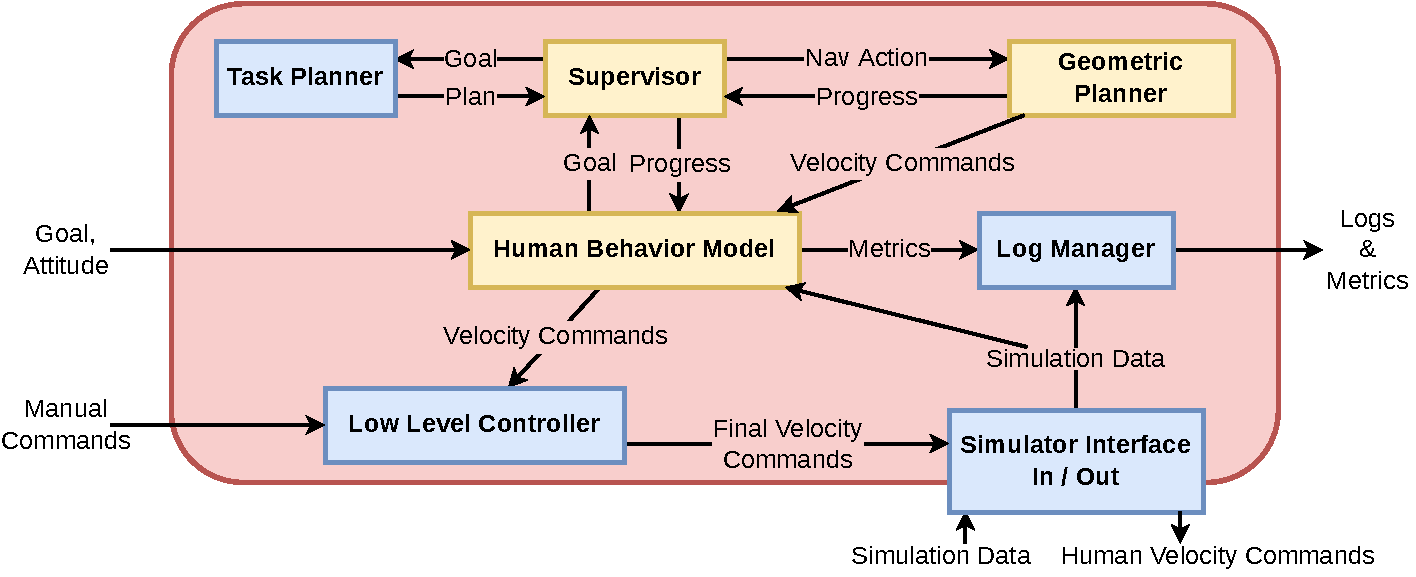
\includegraphics[height=120pt]{Chapter7/inhus_2.pdf}
    \caption{
    The human controller InHuS is depicted with its components and subsystems. 
    }
    \label{fig:inhus_only}
    \vspace{-1cm}
\end{figure}

The macro component InHuS is mainly in charge of controlling the avatar and generating rational behaviors. InHuS itself is made of several components, as depicted in Fig.~\ref{fig:inhus_only}. However, three components, namely HumanBehaviorModel, Supervisor, and GeometricPlanner, constitute the major functional part of InHuS. We discuss each of these major components in detail.


\subsubsection{HumanBehaviorModel}

The HumanBehaviorModel is responsible for most of the rational behavior of the agent. The first role of this component is to manage the goals. Goals can either be received from the Boss component or generated by the HumanBehaviorModel using the same XML file as the Boss. When a goal is selected, it is sent to the Supervisor for execution. 

This component is also responsible for detecting and handling navigation conflicts. Currently, the kind of navigation conflict handled by InHuS is path blockage (e.g. another agent standing in a doorway). While the human agent is navigating, a path to the goal is calculated at regular intervals using Dijkstra's algorithm, and its length is tracked to detect such conflicts. If the tracked path length increases significantly or the path ceases to exist, it could mean that another agent is blocking either the only possible way or the shortest way. When such situations are detected, the plan execution is temporarily suspended, and the agent performs an approach action to get close to the blocking location. This shows the agent's intention to move in a specific direction and might induce the blocking agent to react and clear the way.
Eventually, once the avatar is at a specified distance from the blocking location, set to $1.5m$, the agent stops its approach and actively waits for the path to be cleared.

To generate a lot of different and specific situations, we created what we call \textit{Attitudes}. They are operating modes affecting both goal decisions and reactions toward the other agents. One can activate them through the Boss to generate diversified behaviors of the agent. Some of the \textit{Attitudes} currently implemented in InHuS are the following: 1) randomly picking a new goal, like someone suddenly changing their mind; 2) harassing the robot by constantly going in front of it, like a child would do \cite{nomura2016children}; 3) stopping close to the robot and looking at it for a few seconds before resuming its goal which emulates a curious behavior. 

The final purpose of this component is to build the perception of the human agent based on the map and information about the other agents from the simulator. We build the perception by directly accessing the simulation data rather than adding simulated sensors to the human avatar. Using this perception, we compute the visibility of the human agent and then update the human's knowledge about the robot's position and speed.

\subsubsection{Supervisor}
The Supervisor is a central component as it coordinates different components to execute the plan and achieve the current goal. When the Supervisor receives a goal from the HumanBehaviorModel, it requests the TaskPlanner component a plan to achieve the goal. For now, the plan generation is quite simplistic. For a ``Pose goal'', a plan filled with a single navigation action is generated. For a ``Compound goal'', the navigation and waiting actions sequence is extracted from the XML goal file, and the plan is populated. Despite the simplistic plan generation, this architecture handles complex goals that require several steps to be achieved and emulate human activities.  

The Supervisor then supervises the execution of each action of the plan by sending requests to other components. 
When a navigation action needs to be performed, the Supervisor starts by sampling a random position if the given action radius is not zero. Then, it requests the GeometricPlanner to plan for the target position without considering other agents initially. This way, the avatar starts following the shortest path, and we initialize the conflict detection. After this, the system starts to consider the other agents, and the Supervisor periodically requests the HumanBehaviorModel component to check for potential navigation conflicts. The Supervisor can suspend and resume the plan execution at any time, which can be used to resolve the detected conflicts or to generate specific reactions like the \textit{Attitudes}.

\subsubsection{GeometricPlanner}

The last major component is the GeometricPlanner. This motion planner component receives a target position from the supervisor to reach and generates velocity commands to make the avatar move. This component defines how the agent moves around and adapts its velocity to the other agents in the scene. Since the system is implemented in \acrshort{ros}, we use the standard \acrshort{ros} navigation stack for the GeometricPlanner.

The planner used in InHuS is a publicly available human-aware navigation planner called CoHAN \cite{singamaneni2021human}. It is built over the \acrshort{ros} navigation stack and uses a local planner based on a modified version of the timed elastic band with human-aware properties. 
We benefit from the high-level decision-making of InHuS and the enhanced local navigation of CoHAN with trajectory predictions. Moreover, CoHAN is highly tunable, which helps generate different agent behaviors. 

\subsection{Logs, Metrics and GUI} \label{sec:logs_metrics}

\begin{figure}[!b]
    \centering
    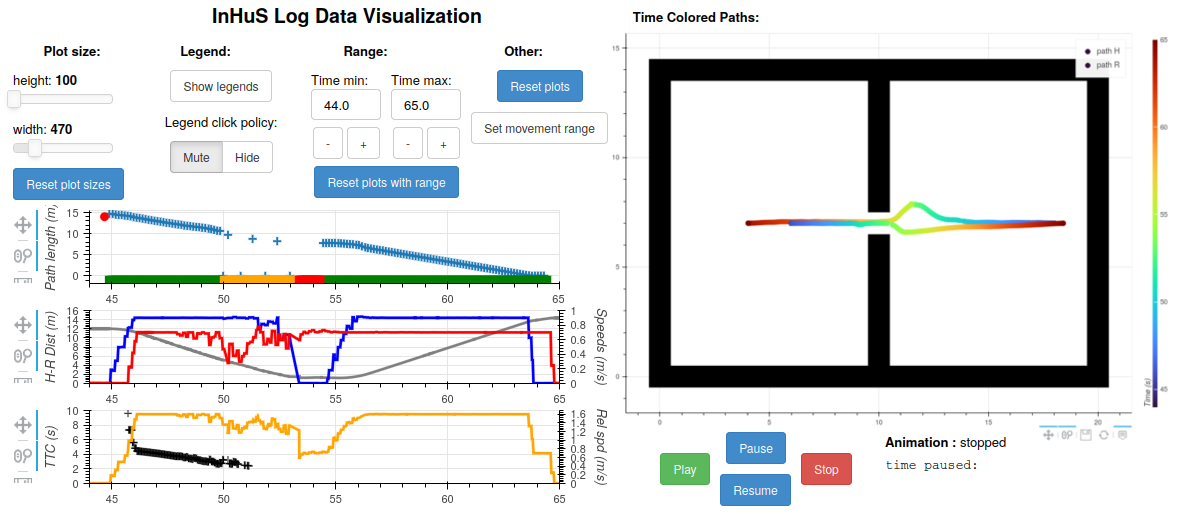
\includegraphics[width=0.8\linewidth]{Chapter7/gui_bis_bis.png}
    \caption{
    An overview of the \acrshort{gui} interface. On the right side, the paths taken by the agents are shown and colored over time. On the left side, several metrics and data produced by InHuS are plotted over time on graphs. Additional widgets help to configure the plots. 
    }
    \label{fig:gui}
\end{figure}

The InHuS system logs the execution data, such as the positions and speeds of the agents, along with some computed metrics. All the logged data is sent to the \acrshort{gui} component, which generates interactive plots. These plots can help evaluate the interaction and, thus, the performance of the given robot controller. The snapshot of the \acrshort{gui} shown in Fig.~\ref{fig:gui} shows two kinds of visualizations. On the right side, there is a colored visualization of the paths taken by each agent. These paths are colored over time according to a corresponding legend that helps estimate an agent's position at a specific moment. The left side comprises several plots showing some computed metrics over time. The first plot is about conflict detection and solving. It shows the path length to the goal computed when checking for conflicts. Without any conflict, the path length should decrease linearly over time. If it's not the case, the avatar has been disturbed during the navigation. This plot also shows the state of conflict of the agent: Nominal (no conflict), approach (conflict detected), blocked (stopped and waiting). The subsequent plots show the speeds of each agent over time, their relative speed, the distance separating them, 
and a metric called time to collision (TTC). This metric estimates the time remaining before the agents collide with their current velocities. We can argue that TTC corresponds to a ``threat feeling'' since a low TTC value corresponds to a high collision threat. Hence, social robots should be tuned not to exceed a minimum TTC value to make humans more comfortable.

\section{Main Results}

In this section, we show some results through a set of experiments to highlight how our system can help challenge human-aware robot navigation systems. First, we discuss the limits of reactive-only systems to strengthen the need for rational avatars. 
Then, we present how our system effectively challenges robot navigation systems, and we interpret the corresponding plots.
Next, we show how the InHuS System can compare the human-aware performances of two different robot controllers.
Finally, we present additional experiments showing the diverse behaviors that can be produced using the \textit{Attitudes} and how ``long runs'' can benefit the development of a robot controller.

\subsection{Limits of Reactive-only Agents}
\label{sec:pedsim_compare}
Most of the current human agent simulations used by the social navigation community rely either on the social force model or ORCA. In order to highlight the limitations of such approaches, we present results obtained with a PedSim\_ROS (or simply PedSim) agent. PedSim is a pedestrian simulator that uses the social force model. It is very efficient for generating crowds to test robot navigation. However, at the individual level, the simulated agents are purely reactive and have no decisional abilities like most pedestrian simulators. 

\begin{figure}
    \centering
    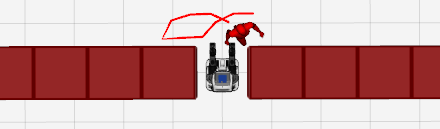
\includegraphics[width=0.4\linewidth]{Chapter7/pedsim_blocked.png}
    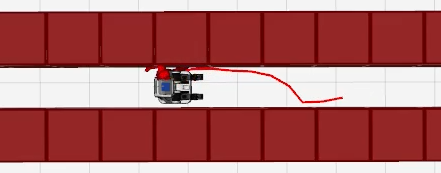
\includegraphics[width=0.4\linewidth]{Chapter7/pedsim_narrow_2.png}
    \caption{
    In the doorway scenario (left), the reactive-only (Pedsim) agent never stops moving while trying to go through the robot, even though its path is blocked. 
    In the narrow corridor scenario (right), the agent squeezes itself between the wall and the robot, colliding with both. 
    }
    \label{fig:limits_reactive}
    \vspace{-0.3cm}
\end{figure}

Consider the doorway scene shown in the left part of Fig.~\ref{fig:limits_reactive}. Both agents have to cross a narrow opening. Here, the robot is blocking the way that the human agent intends to cross. The PedSim agent approaches the robot and tries to push itself through, but it fails due to a very high value of social force. The agent never stops moving and tends to go right or left along the wall before wiggling again just in front of the robot. 
This confusing behavior can make the agent's intentions unclear to the robot planner. 
The narrow corridor scenario, shown in the right part of Fig.~\ref{fig:limits_reactive}, also exposes some limits. In this scene, there is not enough space for the agents to cross each other. The only solution is for one of them to back off. Here, the path is blocked by the static robot. The PedSim agent slowly gets closer and closer to the robot before squeezing itself between the wall and the robot. For some reason, the social forces allowed the agent to pass, unlike the previous example. It highlights that the PedSim agent does not use a defined hitbox or footprint for the agent and relies only on repulsive social forces to prevent collisions. This lack of defined collision shapes makes the agent temporarily pass through the walls and other agents. Consequently, it breaks many intricate scenarios where a rational decision should be taken, resulting in unrealistic situations. Despite being efficient for large spaces or crowds, based on the above observation, we can state that such approaches can lead to confusing and even unrealistic behaviors in intricate scenarios.  

\subsection{Interpretation of Plots with Human-Aware Planner}

The InHuS System is able to generate challenging situations 
and associated logs to allow further evaluation.
Here, we present one such conflict and a detailed interpretation of the corresponding plots. The plots were produced while challenging the CoHAN system in the doorway scenario.

\begin{figure}
    \centering
    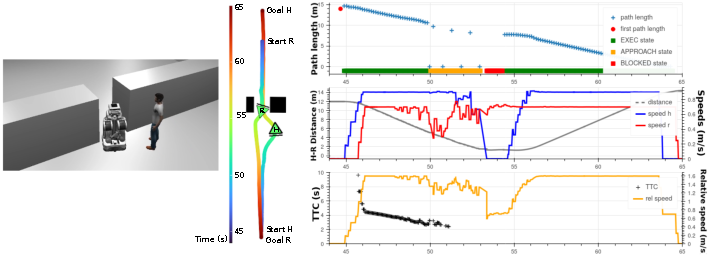
\includegraphics[width=1.0\linewidth]{Chapter7/test.pdf}
    
    \caption{
    A condensed view of the InHuS \acrshort{gui} and MORSE simulator for the doorway scenario with a robot running the CoHAN planner. Several plots depict the detection and resolution of the conflict created. 
    }
    \label{fig:cohan_passage_block}
    \vspace{-0.3cm}
\end{figure}


The robot starts closer to the opening and enters the doorway first. The execution can be analyzed with the metric plots and the time-colored paths of the agents in Fig.~\ref{fig:cohan_passage_block}. We notice that the robot's speed (red line on the second graph) goes down around \SI{50}{\second} as it enters the doorway and creates a conflict. The conflict is detected by InHuS (zero path length = no path), and the agent switches to the approach state (green to the yellow line on the first graph).
The non-zero path length in the approach state corresponds to how the approach is performed. In order to keep moving despite the blocked path, the GeometricPlanner is requested at a defined frequency to plan without considering the robot (all non-zero path length). In between these requests, to check if the path is still blocked, the conflict detection plans while considering the robot (zero path length). When the avatar is at a predefined distance from the blocking robot around \SI{53}{\second}, it switches to the blocked state (red line) to stop and wait for the path to be cleared. Further, the time-colored paths show that the GeometricPlanner made the avatar move aside while approaching to avoid blocking the robot. As a result, the agents were no longer moving toward each other, and thus, there was no longer any collision threat (no TTC values). When there is no more collision threat, around \SI{51}{\second}, the robot's speed starts to increase again. Such behavior is a good sign of human-aware properties and might increase human comfort.

From the plots produced by our system, a lot of useful information can be extracted for improving or evaluating the social robot planner's performance like a) finding ways to decrease the blocked state time for the human, b) maintaining a particular threshold for TTC, c) slowing down near the human, or waiting for the human to cross the door without blocking.


\subsection{Quantitative Comparison between Two Robot Controllers}

Our system can be used to run similar scenarios repetitively to produce robust metric values. These values can help to evaluate the human-aware performances of a given robot controller. To show this, we present a comparison between two different robot controllers. The first one is again the CoHAN system, and the second one is the Simple Move Base (SMB). It uses the \textit{teb\_local\_planner} and the \acrshort{ros} navigation stack with default parameters. We just add an additional process to consider the human agent as a static obstacle to avoid it, so it is not human-aware. Therefore, we should be able to notice a clear difference through the metrics computed by our system. For this comparison, we used three different scenarios: 1) The doorway scenario, where the agents have to cross a narrow opening; 2) the corridor scenario, where the agents cross each other with just enough space; 3) the open space where they cross each other without any environmental constraints. We performed ten repetitions of each scenario for each robot controller. For each set of 10 repetitions, we extracted the mean values of three different metrics and presented them in Table~\ref{tab:compare_robots}. The metrics are the following. First, the time to goal (TTG) is the time taken by the avatar to reach its goal. Second, the minimum distance between the robot and the human (Min HRDist). And the minimum time to collision (TTC). Intuitively, we want the TTG to be as small as possible, the minimum HRDist to be as high as possible, and since a low TTC value represents a collision threat, we want the minimum TTC to be as high as possible. 

\begin{table}[]
    \center
    \begin{tabular}{c|ccc|ccc|}
    \cline{2-7}
                                              & \multicolumn{3}{c|}{\textbf{CoHAN}}                                                                                                                                                                                                      & \multicolumn{3}{c|}{\textbf{SMB}}                                                                                                                                                                                                                 \\ \hline
    \multicolumn{1}{|c|}{Scenario}            & \multicolumn{1}{c|}{\textit{\begin{tabular}[c]{@{}c@{}}TTG\\ (s)\end{tabular}}} & \multicolumn{1}{c|}{\textit{\begin{tabular}[c]{@{}c@{}}min Dist \\ (m)\end{tabular}}} & \textit{\begin{tabular}[c]{@{}c@{}}min TTC\\ (s)\end{tabular}} & \multicolumn{1}{c|}{\textit{\begin{tabular}[c]{@{}c@{}}TTG\\ (s)\end{tabular}}} & \multicolumn{1}{c|}{\textit{\begin{tabular}[c]{@{}c@{}}min Dist \\ (m)\end{tabular}}} & \textit{\begin{tabular}[c]{@{}c@{}}min TTC\\ (s)\end{tabular}} \\ \hline
    \multicolumn{1}{|c|}{\textit{Doorway}}    & \multicolumn{1}{c|}{18.38}                                                      & \multicolumn{1}{c|}{\textbf{2.32}}                                                    & \textbf{1.33}                                                  & \multicolumn{1}{c|}{\textbf{18.26}}                                             & \multicolumn{1}{c|}{2.23}                                                             & 1.16                                                           \\ \hline
    \multicolumn{1}{|c|}{\textit{Corridor}}   & \multicolumn{1}{c|}{\textbf{16.34}}                                             & \multicolumn{1}{c|}{\textbf{2.06}}                                                    & \textbf{1.03}                                                  & \multicolumn{1}{c|}{17.05}                                                      & \multicolumn{1}{c|}{1.59}                                                             & 0.81                                                           \\ \hline
    \multicolumn{1}{|c|}{\textit{Open Space}} & \multicolumn{1}{c|}{\textbf{9.55}}                                              & \multicolumn{1}{c|}{\textbf{2.52}}                                                    & \textbf{1.61}                                                  & \multicolumn{1}{c|}{11.01}                                                      & \multicolumn{1}{c|}{2.34}                                                             & 1.18                                                           \\ \hline
    \end{tabular}
    \caption{Mean values of three InHuS metrics over ten repetitions in three different scenarios and with two different robot controllers. Bold values indicate when the corresponding robot controller performs better than the other.}
    \label{tab:compare_robots}
\end{table}

At first glance, Table~\ref{tab:compare_robots} shows that almost all CoHAN values are better than SMB values. Due to the nature of the doorway environment, the execution of the scenario is quite constrained, which explains why the values are not too different between the two controllers. However, we notice anyway that, compared to SMB, the CoHAN planner tends to keep a greater distance between the agents and a greater TTC (lower collision threat). The time to goal of CoHAN is slightly higher because the robot slows down when crossing and moving in the direction of the human. Thus, in this scenario, it is the price to maintain adequate TTC values.

In the corridor scenario, The SMB robot tends to wait until the last moment to move aside, which is threatening. On the other hand, the CoHAN robot proactively moves to one side of the corridor. As a consequence, it leaves more space for humans and reduces the threat of collision, which is visible in the obtained values. Also, this pro-activity has the effect of smoothing the trajectory of the avatar, which makes this last one reach its goal faster.

Finally, the open space scenario is a bit similar to the previous one. The SMB robot waits until the last moment to avoid the human, which puts the load of the avoidance maneuver on the human. As a result, 
humans have to move aside, extending the duration of their efforts to reach the goal. Also, the SMB robot is closer to the avatar and more threatening on average due to the same behavior. Since the CoHAN robot moved again aside early, its metric values are noticeably better than SMB.

In summary, the human-aware behavior of the CoHAN controller was captured through significant value differences in the computed metrics compared to a non-human-aware robot controller. This implies that our system can help evaluate and compare human-aware robot controllers.

\subsection{Generating Different Behaviors with Attitudes}

\begin{figure}
    \centering
    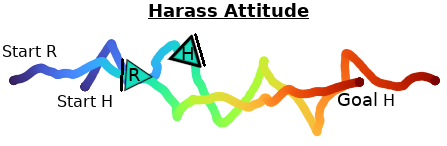
\includegraphics[width=0.6\linewidth]{Chapter7/harass_colored_path_bis.png}
    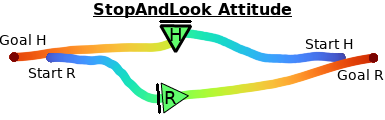
\includegraphics[width=0.6\linewidth]{Chapter7/stoplook_colored_path_bis.png}
    \caption{
    Behaviors obtained by activating the \textit{Harass} and \textit{StopAndLook Attitudes}. 
    With \textit{Harass}, the human is always in front of the robot.
    With \textit{StopAndLook}, when close to the robot, the human stops to look at it for a few seconds.
    }
    \label{fig:attitudes}
    \vspace{-0.3cm}
\end{figure}

By activating \textit{Attitudes}, InHuS is capable of producing more complex behaviors to diversify the conflicts and challenges imposed on the robot.
We present the time-colored paths for the execution of two \textit{Attitudes}: \textit{Harass} and \textit{StopAndLook} in Fig.~\ref{fig:attitudes}. Concerning the \textit{Harass Attitude}, by paying attention to the colors, we see that the human is always in front of the robot that continuously tries to avoid the harassing agent, causing erratic movements. The robot should be able to detect such non-cooperative behavior from humans and act accordingly.
On the same figure, we see the execution of the \textit{StopAndLook Attitude}. The color discontinuity behind the human marker shows how the human suspended its goal to stop and briefly stare at the robot before moving again. A robot that is not proactive enough could be disturbed by the sudden stop of the human, which could be a situation of interest to handle. 


\subsection{Long Run Scenarios}


\begin{figure}
    \centering
    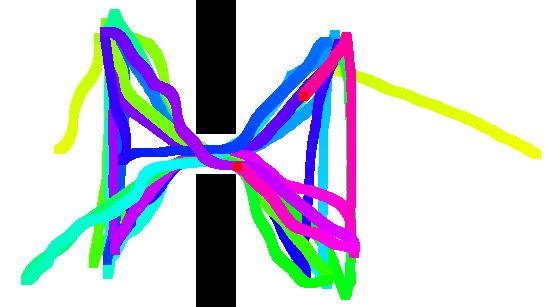
\includegraphics[height=80pt]{Chapter7/TDP_long_run_path.png}
    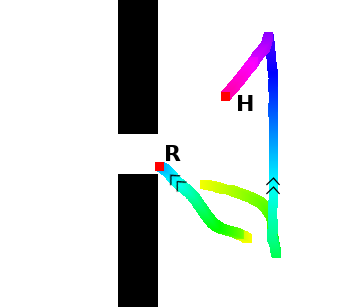
\includegraphics[height=80pt]{Chapter7/TDP_long_run_path_blocked_cropped_final.png}
    \caption{Execution of the long run scenario using the TDP robot planner and InHuS. We see the complete set of time-colored paths on the left. On the right, the same path is cut around when the robot gets stuck in the wall. 
    }
    \label{fig:long_run_block}
    \vspace{-0.3cm}
\end{figure}

The proposed system can help test the stability and robustness of the robot planner by conducting long randomized runs. Indeed, thanks to the Boss component, possibly randomized goals can be sent autonomously to the agents. This can generate unexpected situations and conflicts that can be of interest.
Fig.~\ref{fig:long_run_block} depicts such a test conducted with InHuS and a human-aware robot planner from Kollmitz et al. \cite{kollmitz_time_2015} here referred to as TDP. The agents were made to endlessly loop over four goal positions (each with a $1m$ radius) in reverse order to create as many conflicts as possible. After 3 minutes, the robot got stuck in the wall of the doorway, indefinitely blocking the path of the human. In addition to highlighting problematic situations where the robot does not act as expected, long runs can expose low-level issues like unexpected crashes or memory leaks.




\section{Discussion and Limitations}

Although InHuS provides an autonomous human agent, the agent can be controlled manually if needed. We do not yet provide a handy controller, but velocity commands generated by any means can be sent to the Boss component to control the human. This extends the usability of InHuS as one can use scripted trajectories or motion capture to control the human agent in the simulator.

The proposed system interacts with an external simulator and robot controller. Since the system is mainly implemented using \acrshort{ros}, switching from one simulator to another is straightforward if it has a \acrshort{ros} interface. 
InHuS has specific components to abstract the simulation data format. Thus, just by slightly editing these components, we were already able to run InHuS on three different simulators: MORSE~\cite{echeverria2011modular}, Stage\footnote{https://github.com/ros-simulation/stage\_ros} and Gazebo~\cite{koenig2004design}. Furthermore, any robot controller using the \acrshort{ros} Navigation Stack can be directly used with InHuS.

Simulating intelligent human avatars is a novel field, and only a few works apart from ours have tried to address this limitation. A similar work in ROS2 was recently presented in \cite{perezhunavsim}.
Clearly, the idea of intelligent human agents is of interest to the community, and it is necessary to test social navigation effectively. Like any other system, InHuS has limitations, too. We claim to generate only reactive and somewhat rational behavior, which is still far from natural or realistic human behavior. We currently handle scenarios with two agents only: the human and the robot. We can run scenarios with other human agents, but they will be treated like robots.



\section{Conclusion}

Human-aware social robot navigation is rapidly growing, but the community lacks good human agent simulations to test and debug their systems. The existing reactive approaches offer only limited testing. Through the InHuS system, we proposed a pertinent approach to address this issue. We showed that our system could generate conflicting situations that need resolution by making rational choices. Moreover, all the metrics and data recorded during execution and their visual plots allow us to evaluate the interaction and behavior of the robot. With such evaluation, we showed that we could compare different robot controllers. InHuS can also generate various tunable behaviors that can diversify the situations and conflicts imposed on the robot, and thus, it helps to debug and tune the system. Long runs provide additional potential ways to improve the system.  
\newpage
\thispagestyle{empty}
\mbox{}

\ifdefined\included
\else
\setcounter{chapter}{7} %% Numéro du chapitre précédent ;)
\dominitoc
\faketableofcontents
\fi

\chapter{Interactive Social Multi-Agents Simulation for Robot Navigation: IMHuS}
\chaptermark{Intelligent Multi Human Simulation: IMHuS}
\label{chap:8}
\minitoc

\chapabstract{This chapter presents the IMHuS system designed to choreograph several agents with group movements and social behaviors. This system complements the InHuS system presented in the previous chapter by generating multi-human scenarios. This system has been qualitatively evaluated in an elevator scenario.}

\section{Introduction}

In chapter~\ref{chap:7}, we showed that the InHuS system effectively challenges robot navigation systems in intricate and human-populated environments. However, simulating the interactive agent is computationally demanding. This is why we limited the simulation to only a single intelligent agent. Nevertheless, it is also relevant to general intricate scenarios with several agents. Existing works simulating crowds are only based on a reactive approach and are not necessarily designed to be used to benchmark robot systems.

This is why we propose the Intelligent Multi-Human Simulator (IMHuS). This work is strongly inspired by and complementary to the InHuS framework presented in chapter~\ref{chap:7}. Together with two researchers from the University of Leon in Spain and an intern, we designed this framework based on InHuS. The implementation of this system has been majorly done by the intern. This system allows choreographing several interactive agents with group or individual movements and social behaviors. The individual agents are less complex and demanding than the InHuS one, allowing the simulation to run smoothly.  
This system has been evaluated in the elevator scenario, as defined for the SciRoc competition 2019.

We begin with a comparison between InHuS and this additional work while briefly describing it. After, a more formalized presentation of IMHuS is provided, detailing the information given in the prior comparison. Eventually, the elevator use case evaluation is presented. 


\section{Comparison InHuS vs. IMHuS}

\subsection{Similarities}

Let's first mention the similarities between InHuS and IMHuS work. Like InHuS, this work aims to replicate scenarios involving humans to help social robotics research. Similarly, the simulated interactive agents can be choreographed in a step-based manner to create high-level social behaviors such as waiting for an elevator, getting in and out of it, or standing in front of a store window and moving to the next one. The agents navigate in the environment while avoiding static obstacles and being reactive to moving obstacles to prevent collisions. The agents can also wait for a defined amount of time or turn to look in a direction. Like in InHuS, \textit{Attitudes} can be activated to generate specific behavior, such as harassing the robot. This work also analyzes the execution to compute metrics evaluating the robot's performance in defined social situations. The framework architecture is close to the InHuS one and can also be used with different robotic simulators. Here, it has been implemented with Gazebo.


\subsection{Differences}
However, IMHuS differs from InHuS in several ways. The primary reason is that it manages several interactive agents instead of a unique one in InHuS. Moreover, the agents can exhibit social behavior using explicit social groups. For instance, they can move together to another location or talk in pairs. This requires the new \textit{grouping} actions which create or dismantle groups of humans. An interesting addition is the implementation of asynchronous actions. They differ from synchronous actions, such as navigation/turning/grouping actions, which the agents accomplish during one specific step. Asynchronous actions are not associated with a specific step and correspond to a system of \textit{request} and \textit{response}. Thanks to them, one agent can request another to perform a specific task. For instance, the robot can request a human agent to call the elevator, or if supported, a human agent can request the robot to go somewhere. Not every agent can respond to the robot's requests. For instance, if the robot asks for someone to press the button and no one is around, the request will be dropped, counting as a failure. 

In order to handle several human agents, some simplifications were made compared to the InHuS framework. First, when navigating, IMHuS agents are reactive to other agents. However, their movements are less smooth than the InHuS agent. This is because InHuS couples a frequent global path replanning, taking into account static and moving obstacles and an elaborated local planner to follow the planned path. The local planner used is the Human-Aware robot navigation planner CoHAN, which was presented in the previous chapter. It also allows the agent to have proactive avoidance movements. Also, InHuS uses frequent global path replanning to be even more reactive and to identify sudden path blockage due to other agents. Hence, instead of blindly following the global path it can identify when its optimal path is blocked and switch into a conflicted mode where it reasons on its goal to adapt it potentially. Currently, the agent approaches the blocked spot before stopping to wait for the path to be cleared. 
On the other hand, IMHuS agents do not use any local planner and simply move at a defined speed along the updated global path. This induces human agents to sometimes move abruptly and avoid obstacles at the last moment. 
In addition, IMHuS agents' actions are dictated by the given choreography and do not have individual goal reasoning processes like in InHuS. Hence, IMHuS agents are currently incapable of identifying path blockage situations and may behave erratically in such cases.  

However, this new scheme is still very interesting because of the multitude of human agents generated and the social behaviors that can be choreographed. It can generate relevant and challenging situations for social robotics to handle.


\section{Rational}

The goal of the tool described in this paper is to provide a means to generate scenarios in which predefined social interactions of groups of reactive humans can be used to test the social performance of a robot behavior under evaluation. In the rest of the paper, we will refer to it as \textit{tested robot}. The aim is to use the system to benchmark human-robot interaction behaviors.

The goal of IMHuS, the tool described in this paper, is to provide an open-source toolkit for defining high-level reactive simulated humans with the ability to show the behavior of social groups but using realistic standard robotics simulators that allow researchers to use models of their real robots, both for debugging their algorithms and for benchmarking and repeatability.


\section{Design of a Step-based Social Simulation}
\label{sec:design}

The goal of IMHuS is to standardize the validation of autonomous robot behavior in the presence of people, allowing researchers to design repeatable human social situations. For example, we can define a set of waypoints where different simulated people arrive, meet, and move as a group to a different position, or two people facing each other and then moving together to a different location.

Our proposal considers that both individuals and groups must be included in the simulated environment and that each simulated person should exhibit adaptive behavior in both cases. To achieve this goal, we assume that global path planning for the whole set of agents is more suitable for defining fixed social behaviors than the individual path planning approach. This assumption also serves the purpose of humans exhibiting a typical social behavior that the robot must be able to detect in order not to cross, for example, through the middle of a social group.

A central process can have perfect knowledge of the simulated environment, accessing the real and accurate positions of all the elements of the simulations (obstacles, robots, etc.). It is not designed to emulate an embedded agent since the robot simulation process has to obtain the information through the noise-simulated sensor readings provided by the simulator. This process can use the API of the simulator to get all the information directly, without noise and identification problems (it will know which types of elements are in the simulation and their state). For instance, it does not need to identify if something is ``a door" or if it is opened. The door state is obtained directly from the simulator.


\subsection{Choreography Oriented Simulation}

The constraints and assumptions made for IMHuS are:
\begin{enumerate}
    \item The set of persons $P=\{p_1, p_2, ... p_n\}$ in the environment is defined {\em a priori}, and each person will be unequivocally identified by its ID ($p_i$) during each execution.
    \item The number of locations $L=\{l_1, l_2...,l_m\}$ for these people is also known {\em a priori}.
    \item The number of locations will be greater than the number of people $|L| \geq |P|$.
    \item In a given time-step, only one person can stay at an individual location $l_i$.
    \item Group locations $L^n_i$ will have a maximum number $n$ of individual positions $l_1, l_2, ..., l_n$. For instance, an elevator with four positions will be named $L^4$.
    \item The number of actions is also finite and known.
\end{enumerate}

The tool aims to give researchers a high-level definition of a ``choreography'' of people moving in a social way. For instance, let's consider an example: first, a set of people ($p_1$ to $p_4$) is defined. In the first step, $p_1, p_2$ and $p_3$ must move from their initial positions to a ``group location'' ($L^3$). This joint navigation is represented in figure \ref{fig:diagram} as a continuous top-opening box grouping the three people at time-step $t_0$ and a double arrow labeled with the goal destination. In the same way, $p_4$ will remain in its position but will face a particular direction (30 degrees), indicated by the circle with an arrow. 

 \begin{figure}[h!]%
    \centering
    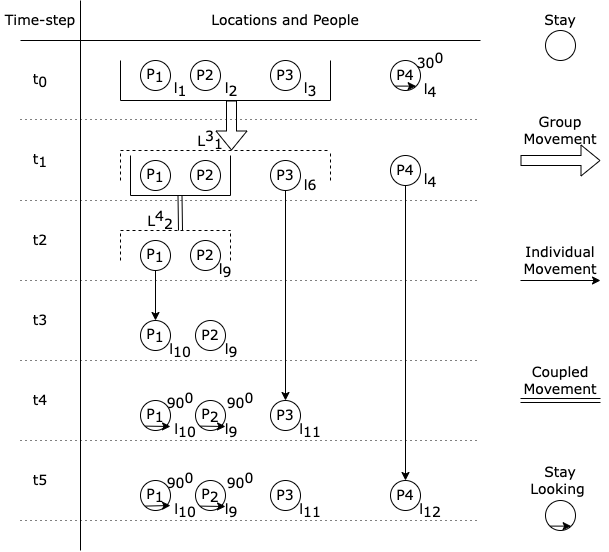
\includegraphics[width=0.7\textwidth]{Chapter8/diagrama.png}
    \caption{Schematic representation of the definition of a social navigation choreography}
    \label{fig:diagram}
\end{figure}

At $t_1$, $p_1$ and $p_2$ engage in a pair-move to $L^4$, while $p_3$ and $p_4$ initiate individual moves, indicated by a single arrow. A pair-move is a specific type of group move included in the design because it is usually the most common and can be considered the smallest group unit. At $t_2$, the two persons moving as a pair would have reached their destination, and $p_1$ will initiate its movement towards $l_{10}$, while $p_2$ remains in its current position with no particular orientation (indicated by a circle with no arrow), and $p_3$ and $p_4$ continue to navigate to their targets.

$p_1$ at $t_2$ begins to move individually towards $l_{10}$, which reaches at $t_3$ while $p_3$ and $p_4$ continue to execute their solo movement. $p_3$ reaches $l_{11}$ at $t_4$, when $p_1$ and $p_2$ begin to face in the same direction. Finally, at $t_5, p_4$ reaches its destination ($l_{12}$) and the choreography ends.

Time-step ($t_i$) in figure \ref{fig:diagram} means ``\emph{choreography steps}'', that is, significant moments for the definition of the simulation. It does not refer to a magnitude measured by a clock. We will refer to them as \emph{steps}, which is an increased ordered sequence of discrete points in time at which a given set of events has to occur. For example, $step_0$ usually specifies the initial state of all the elements of the simulation, i.e., the position of the robot, human', and the other elements. A typical step specifies a set of actions that are initiated at that instant, a navigation task for one of the humans, for instance, at $step_1$ ($t_1$ in figure~\ref{fig:diagram}).


This is the type of simulation that the tool should be able to generate. Figure~\ref{fig:imhus_architecture} shows the general architectural framework. This tool receives the definitions of the social scenarios in a definition file (an XML in its current version). It then manages the simulation, obtains the simulation data, uses existing libraries and other tools (such as $move\_base$ to calculate trajectories in \acrshort{ros}), and finally generates the log data for evaluation.

\begin{figure}
    \centering
    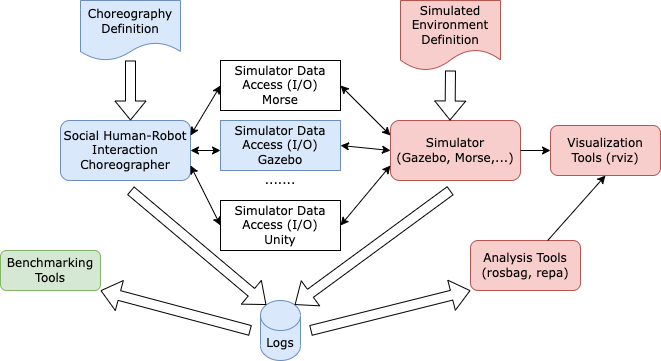
\includegraphics[width=\textwidth]{Chapter8/architecture.png}
    \caption{Global simulation architecture. Red signifies existing tools. Blue components are those described in this paper. Green signifies ongoing development. Uncolored boxes are alternative simulators under consideration.}
    \label{fig:imhus_architecture}
\end{figure}

The definition of the choreography shown in the upper left of the figure \ref{fig:imhus_architecture} is defined in XML. The design allows five types of \emph{basic actions} that the \emph{agents} (simulated robots or simulated people) can perform:

\begin{description}
    \item[Navigation actions]: Those actions modify the global pose of the agents in the environment. Typical actions in this group are $GoToPose$ and $Wait$.
    \item[Turning actions]: Actions related to the facing of the agents, such as $LookAt$ and $Turn$, depending on the way the action is specified.
    \item[Grouping actions]: These actions manage the creation and dismantling of groups.
    \item[Attitude actions]: Actions modeling the high-level behavior of the agent. For instance, a simulated human can be ordered to \textit{harass} the robot.
    \item[Synchronous actions]: Actions related to the environment to be accomplished by an agent during one specific step of the simulation. They have been standardized as $publish$ and $subscribe$.
    \item[Asynchronous actions]: Actions related to the environment and not associated with a specific step in the timeline of the simulation. They have been standardized as $request$ and $respond$.
\end{description}

These actions can be applied to a single agent or a group. Basic actions can be integrated into a $compound\_task$. For defining these actions, the following components are used:
\begin{itemize}
    \item \emph{map}: corresponds to the ``world" where the simulation will happen. Inside the map, a set of \emph{objects} can be defined, specifying their individual ID.
    \item \emph{poses}: correspond to the ``location" used in figure \ref{fig:diagram}. They comprise the $x,y$ position and orientation $\theta$ and a $radius$ of tolerance for the motion planner to consider that the goal has been reached.
    \item \emph{agents}: that can be either $robots$ or $humans$, each of them identified by an unique ID. They are given an initial pose where they appear in the world.
    \item \emph{groups}: they can be created and dismantled during the simulation
\end{itemize}

The evolution of the simulation is based on steps, as described in the previous section. The regular steps are synchronous, but there is an asynchronous step for interacting with the tested robot:
\begin{itemize}
    \item A scenario is composed of a set of regular steps and a singular asynchronous step.  
    \item Steps are made up of different actions like navigation, grouping, etc.
    \item Every action of a step is executed {\em at the same time}, meaning that the actions are executed in simulated parallelism. 
    \item One step ends when all its actions have finished.
    \item The asynchronous step runs in parallel to the execution of the synchronous steps. 
    \item The scenario ends when the last regular step ends.
\end{itemize}

\section{Implementation}
\label{sec:implementation}
In the current version, choreographies are defined in an XML file that includes four main sections:
\begin{itemize}
    \item Map = poses and objects. Example: poses definition.
    {\footnotesize
        \begin{quote}
        \begin{verbatim}
<poses> ::= <pose> (<pose>)* ;
    <pose> ::= <poseID> <x> <y> <theta> <radius> ;
        \end{verbatim}
        \end{quote}
    }
    \item Agents = humans/choreographed robots with their initial poses and groups with their composition. Example: group definition.
    {\footnotesize
        \begin{quote}
        \begin{verbatim}
<groups> ::= (<group>)* ; 
    <group> ::= <groupID> <pair> (<human> (<human>)*) ;
        <pair> ::= <pairID> <human> <human> ;
        \end{verbatim}
        \end{quote}
    }
    \item Tasks = generic actions. Example: compound tasks and look-at action definition.
    {\footnotesize \noindent
        \begin{quote}
        \begin{verbatim}
<compound_tasks> ::= <compound_task>* ;
    <compound_task> ::= <compound_taskID> <action> (<action>)*;
<lookAt_action> ::= <actionID> (<humanID>|<robotID>|<objectID>); 
        \end{verbatim}
        \end{quote}
    }
    \item Scenarios = step elements of synchronous steps and asynchronous steps. Example: scenario definition. 
    {\footnotesize
        \begin{quote}
        \begin{verbatim}
<scenario> ::= <name> <step> (<step>)* (async_step);
    <step> ::= <stepID> <stepElement>; 
        <stepElement> ::= <agentsID> <pose>|<compound_task>;
        <agentsID> ::= <humanID>|<robotID>|<pairID>|<groupID>;
    <async_step> ::= <respond_event_action>;
        \end{verbatim}
        \end{quote}
    }
\end{itemize}

The prototype has been implemented as a new version of the InHuS tool (\cite{favier_SSC}), which connects to the Gazebo simulator to obtain information about the world. It uses the \emph{move\_base} \acrshort{ros} to generate the global plan for each agent and updates the positions of each agent in the next step of the simulation accordingly. The new version is capable of handling the navigation of multiple agents (humans) in parallel while managing conflicts and completing individual tasks as in the previous version. It also provides an updated graphical user interface for repeatedly selecting and executing scenarios defined in the XML file.

The IMHuS tool shown in Figure~\ref{fig:imhus} has been structured in three layers: the IMHuS layer (in blue), its configuration in the application layer (in yellow), its communication with the simulator and \acrshort{ros} (in red). The robot whose behavior would be tested in the tool has also been included (in violet).

  \begin{figure}[ht]%
     \centering
     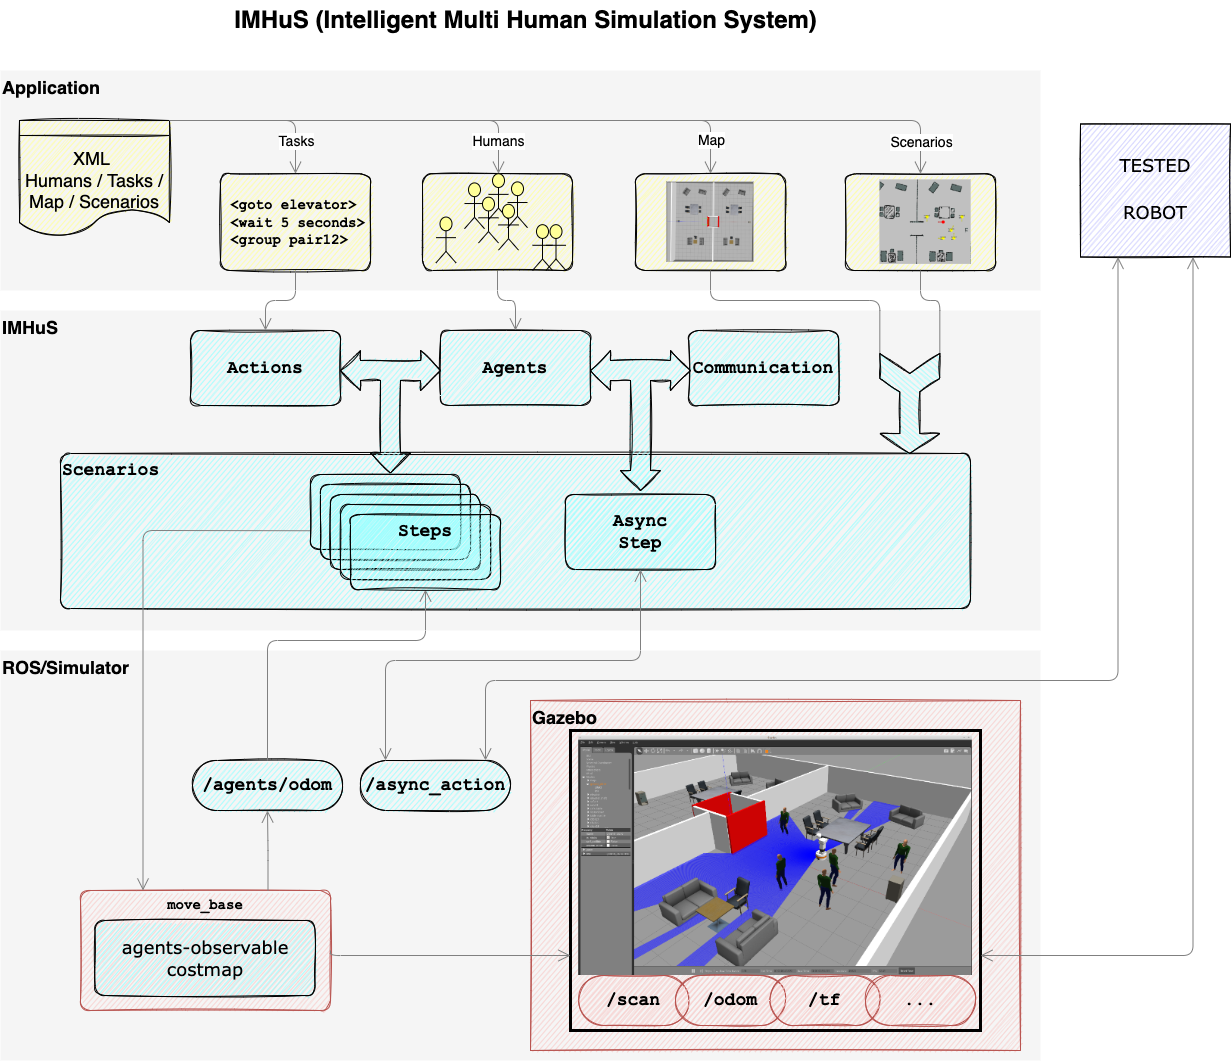
\includegraphics[width=1\textwidth]{Chapter8/IMHuS.png}
     \caption{Structure of the new IMHuS tool.}
     \label{fig:imhus}
 \end{figure}

\begin{description}
    \item[Application layer] This layer includes the XML configuration file needed to use IMHuS by defining its main components: map, agents, tasks, and scenarios. The map includes all the locations of the agents to be used during the choreography and those of static objects. These locations are represented as poses, and a name is assigned to each. The description of the agents includes the name, and initial position of all humans and robots choreographed, as well as the name and composition of the groups that will appear at any step. Generic tasks are described with no specific subject to perform them so that several agents can reuse them. Lastly, the scenarios describe the choreography steps. Each step includes a set of tasks assigned to a particular agent or a group. They are the step elements. 
    \item[IMHuS layer] The tool interprets the information contained in the XML configuration file to represent the tasks as actions and the humans/robots as agents. When the scenarios are run, a command combines actions with agents for every step element. The commands concerning each agent are executed in a separate thread inside a step. The step finishes when all the threads are done. This is the way simultaneous movements of agents are achieved. 
    This is the behavior of the tool for the choreography, but considering that the tested robot will be present, there must be a way for it to communicate with the simulation agents, just as it would happen in the real world. The asynchronous step is responsible for this task. At any point, the tested robot can ask something, for example, to press the elevator button. This action would be done through the communication module and answered by the agents in the simulation in this asynchronous step by a response action. Not every agent can respond to a request from the tested robot. For instance, if the robot asks for someone to press the button and no one is around, the request will be dropped, counting as a failure.
    \item[ROS/Simulator layer] IMHuS uses this layer to place the agents in the simulation, ask for the trajectories to move them around, and communicate with the tested robot. The agents are placed in the world as obstacles so that they are avoided when \texttt{move\_base} is asked for a new path. The costmap obstacle layer has been modified to obtain what we call the \textit{agents-observable costmap} that IMHuS needs.
    \item[Interface of the tested robot] The way to include the software of a robot in the simulator for its social behavior to be tested would be through the simulator, here Gazebo. Outside the simulator, the only communication would be through asynchronous actions. They allow the robot to send a request action to be answered by a response action from one agent of the simulation.
\end{description}


\section{Use Cases}
\label{sec:useCases}


This module is available as Open Source, and it has been evaluated in the elevator scenario, as defined for SciRoc competition (\href{https://github.com/LAAS-HRI/IMHuS}{IMHuS repository link}). %In this scenario, the robot has to be able to take an elevator in the presence of people.

An elevator scenario will be used to show a running example of the behavior of the IMHuS system with a tested robot and also to explain the communication between the \textit{tested robot} and the agents of IMHuS (video available at \href{https://github.com/LAAS-HRI/IMHuS/videos}{this link}). The proposed scenario includes five human agents and the \textit{tested robot}, whose goal is to go to the second floor. In order to do that, it has to ask a human agent to push the elevator button. Figure~\ref{fig:take_elevator_video_1} shows the initial situation where the \textit{tested robot} is approaching the elevator, human\_2 is walking, and the rest of the humans are idle.

\begin{figure}[!ht]
  \centering
  {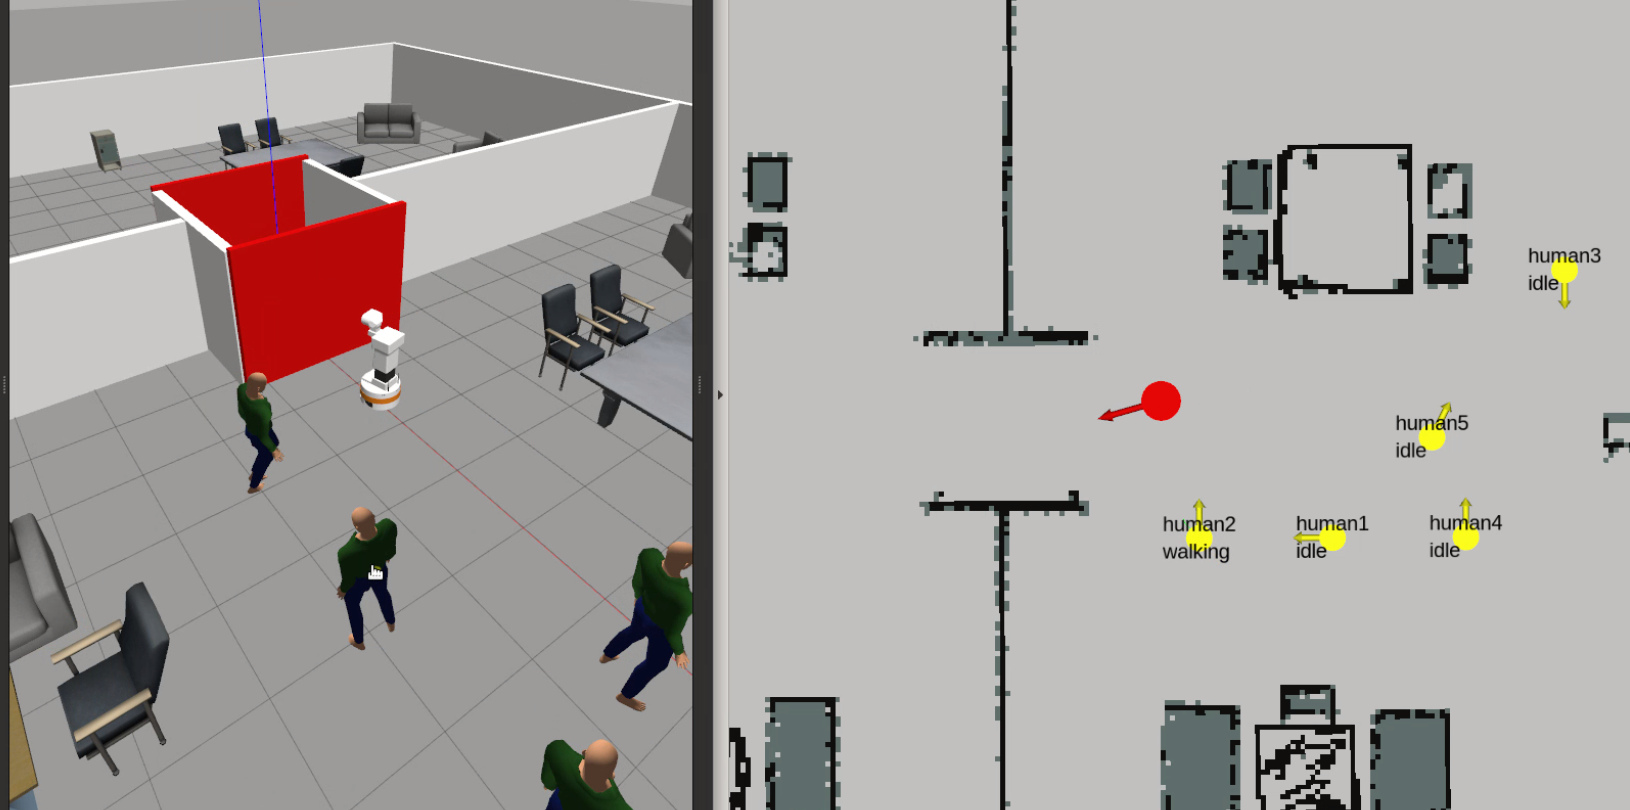
\includegraphics[width=1\textwidth]{Chapter8/seq1.png}}\\
  \caption{Initial situation.}
  \label{fig:take_elevator_video_1}
\end{figure}

Once the \textit{tested robot} gets to the elevator door, it requests that one of the humans perform an action. In order for a \textit{tested robot} to trigger an action in IMHuS, it has to publish a specific message type on the \texttt{async\_action} topic (see Figure~\ref{fig:imhus}). Doing so triggers an asynchronous action response from IMHuS. This message should contain the time of emission, the name of the agent requesting it, the pose of this agent, and the name of the task it is requesting. If the scenario includes in its configuration an asynchronous action response corresponding to the requested action, that action is triggered on the human's side.

At this point, two different things can happen. If there is no human close enough to the \textit{tested robot}, or there is a human but it is not in an idle state, no one will respond to the request, and it will be dropped, as Figure~\ref{fig:take_elevator_video_2} shows.

\begin{figure}[!ht]
  \centering
  {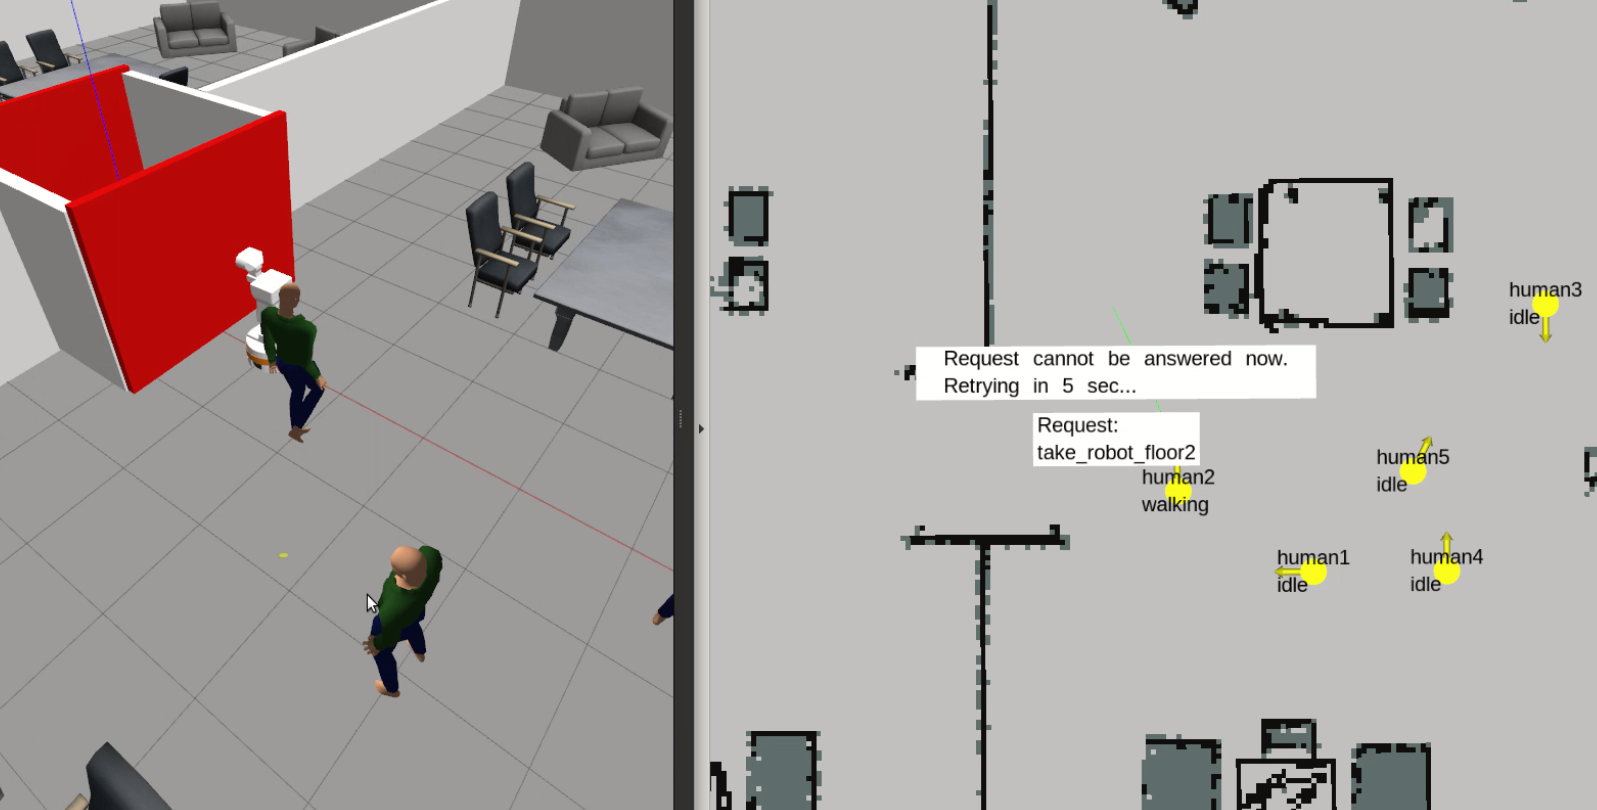
\includegraphics[width=1\textwidth]{Chapter8/seq2.png}}
  \caption{Request dropped.}
  \label{fig:take_elevator_video_2}
\end{figure}

The \textit{tested robot} repeats the request every five seconds until human\_2 enters an idle state and responds to the request. Figure~\ref{fig:take_elevator_video_3} shows this moment of the simulation. When an asynchronous action request is triggered, IMHuS periodically checks if one human is able to respond. The requirements for a human agent to respond are to be in the idle state and within a $3m$ radius from the \textit{tested robot} position when it requested the action. If several human agents can accept the task, the task will be assigned to the closest human.

\begin{figure}[h]
  \centering
  {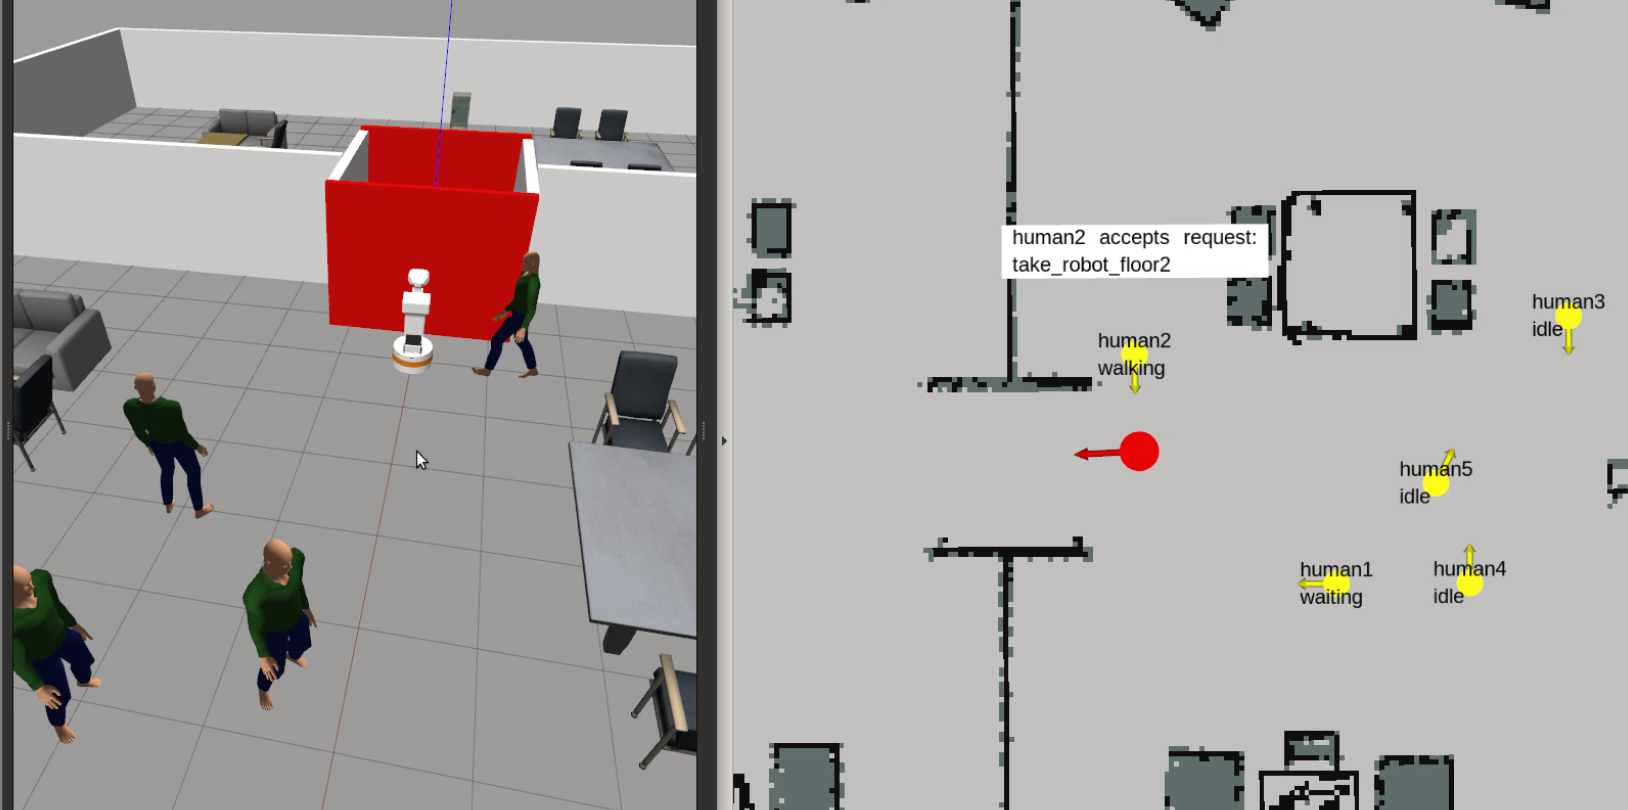
\includegraphics[width=1\textwidth]{Chapter8/seq3.png}}\\
  \caption{Request accepted by human2.}
  \label{fig:take_elevator_video_3}
\end{figure}

Figure~\ref{fig:take_elevator_video_4} shows the final situation where the \textit{tested robot} has reached the second floor, simulated in the scenario as the room on the other side of the elevator.

\begin{figure}[h]
  \centering
  {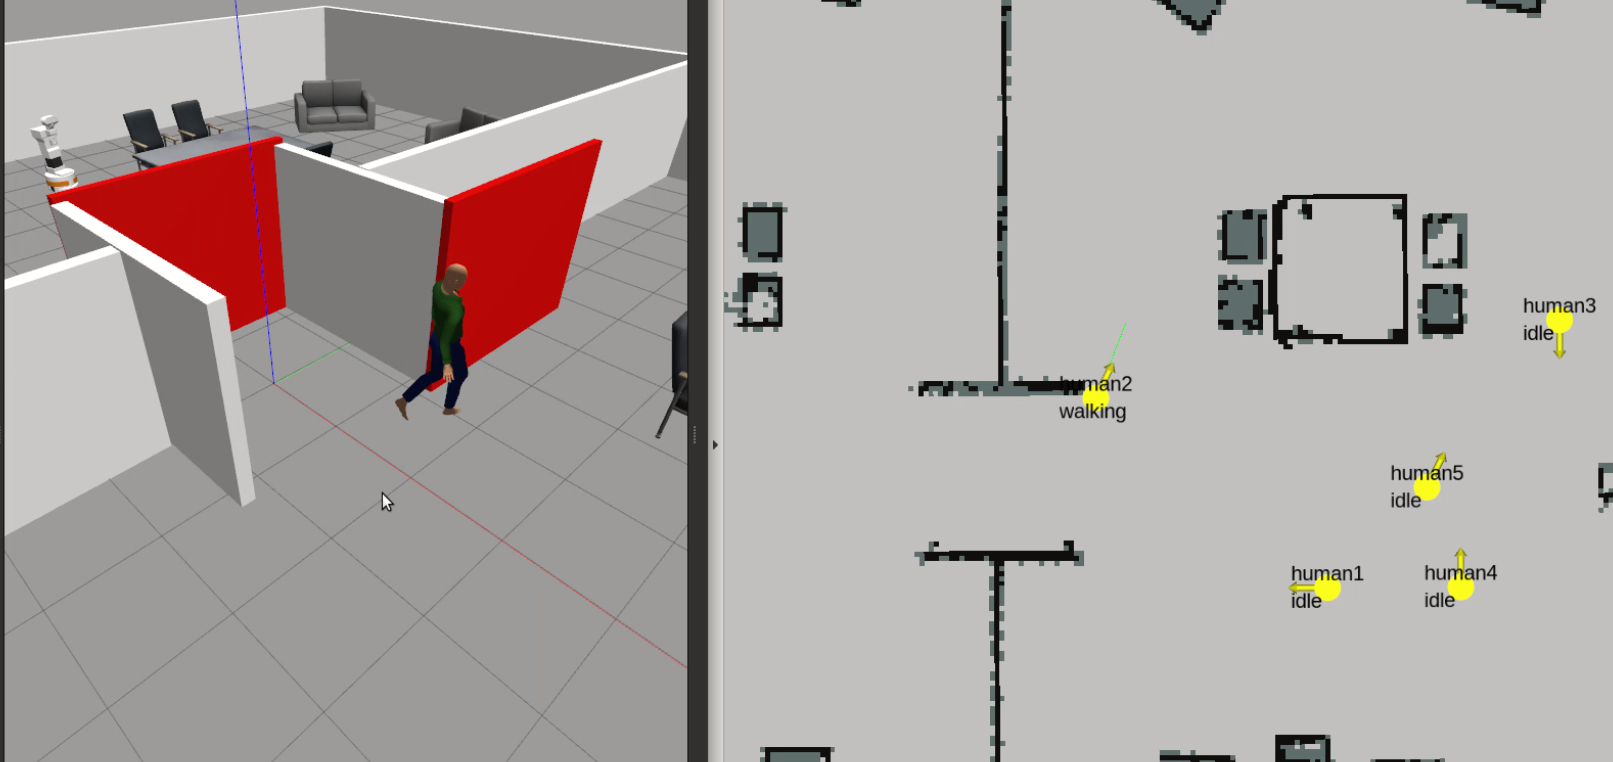
\includegraphics[width=1\textwidth]{Chapter8/seq4.png}}\\
  \caption{Final situation. \textit{Tested robot} in second floor.}
  \label{fig:take_elevator_video_4}
\end{figure}

\clearpage

\section{Conclusions and Future Work}
\label{sec:conclusions}

The proposed tool, IMHuS, offers the possibility to create a realistic and challenging simulated environment in which groups of humans can be choreographed to evaluate the behavior of a \textit{tested robot}. Different scenarios can be easily created using an XML configuration file in which social situations can be defined to measure the behavior of \textit{tested robots} in a replicable environment. Furthermore, human agents are programmed to respond to interactions related to the particular situation of each scenario and their communication with the \textit{tested robot}. 

IMHuS's code is available as Open Source in the  \href{https://github.com/LAAS-HRI/IMHuS}{IMHuS repository}. The current version has been implemented for the Gazebo simulator, but the design presented in section~\ref{sec:design} can be easily migrated to other simulators, such as MORSE or Unity. The tool could be used to benchmark competitions such as SciRock or RoboCup as a previous step for the teams before getting to the physical robot challenges. To create a new scenario with IMHuS, all that is needed is a map and the configuration file to choreograph the human agents. The software has been designed to easily support the addition of both new tasks to be performed by the humans and new interactions between them and the \textit{tested robot}.

One of the ongoing developments is the automatic generation of simulation metrics such as the distance between the robot and the agents, time-to-collision, etc. Another line of work is the extension of basic actions, especially towards the social behavior of groups of agents. Last, IMHuS is being tested with CoHAN \cite{singamaneni2021human}, a human-aware robot navigation planner, to challenge CoHAN under several human-robot interaction settings. From this, we plan to identify the areas of improvement for human-aware navigation planners and provide a benchmark for testing these planners.


\chapter*{Conclusion}
\addstarredchapter{Conclusion} 
\markboth{Conclusion}{Conclusion}

\mysection{Contributions}

In this thesis, we addressed the challenge of enhancing the decision-making of robots to ensure seamless collaboration with a human partner. Several contributions have been proposed, contributing to robotic human-aware task planning on the one hand and to robot navigation by simulating social interactive agents on the other. 

To better capture my contributions, we presented in Chapter~\ref{chap:1} the specificities and the multidisciplinarity of the Human-Robot Interaction field and the Human-Robot Collaboration subfield. Eventually, we presented state-of-the-art approaches in HRC task planning and robot navigation. 

\subsection*{Task Planning Conclusions}

Task planning for human-robot collaboration is a research topic of high interest to which numerous works have contributed. However, most of these works do not consider distinct agent models and, thus, do not consider different beliefs, action models, or goals. Moreover, works from the literature tend to produce a joint plan that must be shared and accepted by the human, assuming in a way that the human is controllable and must follow the produced plan, which is an approach close to multi-robot planning. Finally, existing approaches usually assume the agents have already established a shared goal. However, scenarios where the robot should decide `when' and `how' to start the collaboration are also relevant to be explored. 
Hence, there is a lack of task planning approaches preserving the human's latitude of online decisions while collaborating efficiently to solve both shared and individual tasks. 


In Chapter~\ref{chap:2}, we presented the HATP/EHDA human-aware task planner designed to address the highlighted gap in the literature. After participating in its development, this planning scheme became a laboratory to explore relevant human-aware task planning challenges, leading to two main contributions. 

In Chapter~\ref{chap:3}, we proposed models and algorithms to integrate concepts of Theory of Mind in the planning process of HATP/EHDA and plan the robot's actions appropriately. 
The main idea is that agents only update their beliefs from observable facts in their surroundings or by observing a co-present agent acting. 
More precisely, we modeled observability as follows. First, each fact describing the state of the world is associated with a place, which can be symbolic. The agents are situated and can move from one place to another. When situated in the same place, two agents are said to be co-present, and an agent and a fact are said to be co-located. Second, each fact is associated with an observability type stating if the fact is observable or not. For instance, the color of an object is observable and can be learned if situated near the object. However, the presence of salt in water or the temperature of an object is not observable but can be inferred in certain situations.
Based on these models, we propose two rules to update agent beliefs. First, an agent learns from observing a co-located observable fact. These updates are done through a systematic Situation Assessment process inserted in the planning process of HATP/EHDA and executed after each planned action. Hence, the agent will automatically observe and learn from its surroundings. For instance, when moving to another room, the agent's beliefs will be updated with (only) observable facts located in the other room.  There is no need to script this assessment in the `\textit{move}' action's effects. On the other hand, an agent learns from observing a co-present agent performing an action (including the agent itself). In this case, the agent's beliefs are directly updated with all action's effects, including effects affecting non-observable facts. This rule models the inference that humans internally perform when observing their surroundings. For instance, if the human observes the robot adding some salt to the water, they can naturally infer that some salt is now in the water, although it is not observable.
Using those two rules, we can maintain human beliefs more precisely to predict their behavior better and detect false beliefs that may be detrimental to collaboration. Finally, we solve \textit{relevant} false human beliefs as follows. First, from the erroneous facts present in the human beliefs, we identify which ones must be corrected to solve the task. Then, a communication action correcting the minimal number of false beliefs is inserted into the robot's plan, potentially leaving some non-detrimental erroneous facts in the human beliefs. As a second possible solution, we then check if the relevant false beliefs are due to a non-observed robot action. If so, we create another possible plan where the robot delays the relevant action until the human can observe its execution, avoiding the creation of the false belief. 
We evaluated this approach empirically using three domains, including shared tasks, several places, and non-observable facts. We showed that the proposed models and algorithms allow us to solve a broader class of problems than the original HATP/EHDA planner. Moreover, our relevant false beliefs detection and minimal communication already avoid systematic communication, and considering delaying robot actions reduces the communication rate of the solution plan produced even more. 


In Chapter~\ref{chap:4}, we proposed another contribution bringing planning and execution closer. We proposed a step-based model of concurrent and compliant joint action execution. 
This model describes several possible coordination of the agents, including the four following cases: 1) the human decides to perform any desired action and the robot complies by executing its best non-conflicting action in parallel; 2) the human decides to be passive and let the robot act alone; 3) the human is acting alone while the robot remains passive; 4) the human decides to let the robot decide and start acting purposely, then the human accompany the robot with a concurrent non-conflicting action.
We use an abstracted version of this model to guide our search and explore further concurrent courses of action, allowing the robot to anticipate possible execution conflicts. 
The exhaustive exploration produces a directed acyclic graph where each path from the root to a leaf is a sequence of concurrent human-robot actions leading to the goal. From this graph produced offline, the robot's behavioral policy is extracted using an estimation of the human preferences regarding the joint task. These preferences can optimize various objectives, for instance, minimizing the human efforts, finishing the task as soon as possible, or freeing the human as soon as possible.  
This policy indicates the best concurrent robot action to satisfy the estimated human preferences in every state and for each possible human action. This allows the robot to comply optimally with any human online decision.  
Moreover, this extraction is light and can be done online. As a result, as the execution progresses, the estimated human preferences can be reevaluated, and the robot policy can be updated accordingly on the fly.
To evaluate our approach, we used BlocksWorld scenarios where the human and the robot had to collaborate to stack colored cubes to match a given goal pattern. 
As a first step, we evaluate the approach by symbolically simulating possible executions, following the abstracted model of execution proposed. To highlight the compliance endowed to the robot, we simulated erroneous estimations of the human preferences, making the robot's behavior more or less adversarial to the human preferences. However, the robot always aims and helps to fulfill the shared task, but not necessarily in the way the human would have preferred. The results showed that despite erroneously estimated human preferences, the actual human preferences are correctly satisfied overall because the robot constantly adapts to and follows human decisions. 
To further validate the approach, we presented the user study we conducted in Chapter~\ref{chap:6}. This study is based on an interactive simulator created explicitly for this purpose presented in Chapter~\ref{chap:5}. This simulator includes a refined and implemented version of the model of execution used as an execution controller to supervise the robot's policy execution. This simulator allowed human participants to collaborate with a simulated Tiago robot through mouse control. We compared our approach with a contrasting baseline where the robot always imposes its decisions on the human. By recording execution data and requesting participants to answer a questionnaire, we showed that our approach performed and was appreciated significantly better than the baseline. Over the different scenarios, our approach permitted to satisfy the human preferences significantly better and the baseline. 
Moreover, the most significant differences using our approach are that the participant perceived the Interaction as more Positive, the Collaboration as more Adaptive and Efficient, and the Robot's Decisions as more Appropriate and Accommodating.    

\subsection*{Social Navigating Agents Simulation Conclusions}

On the other hand, navigation is a fundamental skill for a robot. State-of-the-art methods are efficient for static, dynamic, and unknown environments. However, navigating in human-populate environments is still challenging. Various approaches address the human-aware navigation subject, but only a few recent works propose tools to challenge, test, debug, and evaluate robot human-aware navigation systems. Without such simulation tools, preliminary experimentation and debugging must be achieved using a real robot, which is slow and burdensome. 
Most existing simulated interactive agents are based only on reactive approaches, making them suitable for crowded scenarios but limited and unrealistic in intricate ones. 
Thus, there is a lack of simulated interactive agents endowed with some decision-making processes allowing them to resolve more realistically intricate scenarios, like path blockage or narrow corridor crossing.

In Chapter~\ref{chap:7}, we proposed a complete system to simulate agents endowed with decision-making capabilities. The InHuS architecture has been designed to be generic, but we implemented it as a first step for the navigation use case. 
This system aims to challenge and evaluate robot navigation in intricate human-populated scenarios. It simulates an environment including a robot and a human avatar. The robot is controlled with a navigation system to challenge and evaluate. The InHuS system controls the human agent. Scenarios, including start position and a goal for each agent, can easily be defined and reproduced. The avatar can be given compound goals corresponding to sequences of navigating and waiting actions to simulate complex human activities. 
The avatar uses the CoHAN human-aware navigation planner to navigate, producing proactive and legible trajectories. 
Additionally, the avatar detects when the robot blocks the shortest path to its goal. Instead of following another path, the system switches to a conflict mode, makes the avatar approach, and eventually stops near the blocking spot to show its intention to cross. Once the path is cleared, the avatar proceeds with nominal navigation.
To diversify the challenging situations, \textit{Attitudes} can be defined in the system. They are modes that can be activated anytime, influencing the avatar's goals and reactions to the robot. Through these modes, we can simulate curious, distracted, and non-cooperative humans. There is also an \textit{Endless} mode, making the agents repeatedly move to defined agent-specific positions. This is useful to generate unexpected situations and test the robustness over time of the robot system. Another interesting feature is the ability to randomize all position goals. The final goal position is randomly sampled around the original within a given radius. 
To propose realistic behavior, the system computes the visibility of the avatar and updates the robot's known position only when it is observable. 
Finally, the system records execution logs, such as agents' positions, speeds, and additional computed metrics. Among these metrics are the Time To Collision, the estimated time until the agents collide, and the Surprised metrics. The latter helps identify sudden close robot appearances from behind the avatar. All these data are plotted on an interactive visual interface, providing real time feedback while running the system.
We evaluated this system using two robot navigation systems. One is CoHAN, with human-aware properties. The other is close to the default ROS robot navigation stack, without human-aware properties.
After running both systems in a few challenging scenarios, the data gathered with InHuS indicates that, as expected, CoHAN exhibited significantly better human-aware properties than the default system. This suggests that InHuS can effectively challenge and evaluate the human-aware properties of a robot navigation system. 

Eventually, in Chapter~\ref{chap:8}, we proposed the IMHuS system, a complementary approach to the InHuS system. Indeed, InHuS is limited to simulating a single avatar. IMHuS permits to choreograph several agents and the production of group and social behaviors. The IMHuS agents do not have individual decision-making capabilities. However, this framework allows producing intricate scenarios with multiple human agents to challenge robot navigation systems. Hence, it is an interesting solution between intricate single-agent scenarios and wide crowded scenarios. We showed the effectiveness of the approach in an elevator scenario. 


\mysection{Limitations and future works}

In this section, we discuss the limitations of the contributions presented in this thesis and the possible future works they suggest. 

\subsection*{Theory of Mind in Human-Aware Task Planning}

% Currently limited. 
% No uncertainty in robot knowledge: we could evaluate the confidence level of information, and rely only of high confidence one.
% No uncertainty in estimated human beliefs: assume worst case scenario, we could anticipate scenario where the human correctly anticipated robot actions and keep track of several possible world (epistemic planning)
% We could add more reasoning: logical (DEL, if A or B is true, and I know not B, then A is true), causal (if action B can only be performed after A, and I see some B effects, then A has been executed)
% Communication: For now we are able to identify the minimal relevant information to communicate, however, not when to communicate it. Currently, we comm at last moment, just before the estimated divergence to occur. Could be interesting to identify the best place to comm, could be before human even leave the room.

% %%%%%%%%%%%%%%%%%%%%%%%%%%%%%
% *****************************
% %%%%%%%%%%%%%%%%%%%%%%%%%%%%%


There are some limitations to the approach presented in Chapter~\ref{chap:3} that introduce Theory of Mind concepts in the HATP/EHDA planner.
First, we do not consider uncertainties in the robot's knowledge about the world. Despite being linked to agent knowledge, and thus chapter~\ref{chap:3}, this limitation is common to everything linked to HAPT/EHDA. Indeed, since the planner is part of the robot, there is no choice but to rely on the robot's knowledge about the world, hoping it is correct. An interesting future work could be to abstract the perception layer of the robot and associate each state variable to a confidence level. This confidence level would indicate how much the corresponding fact is sure. Then, the robot could rely only on the high-confidence ones. 

Secondly, we do not consider uncertainties in human beliefs. We assume the worst-case scenario where humans do not know about facts they did not see. However, considering the pasta cooking example of Chapter~\ref{chap:3}, the human could assume that the robot effectively did its work while being away fetching the pasta, and thus, the human could believe that there is salt in the post even without seeing the robot's action. Keeping track of such different possible worlds is an approach used in epistemic task planning. It would be an interesting future work that we already started investigating in our lab. 

Another promising future work is to add more reasoning and inference processes to the planning process. We have already introduced the situation assessment process, updating agents' beliefs concerning their observable surroundings. However, adding logical reasoning and deduction would be interesting, like in the Dynamic Epistemic Logic in \cite{bolander_gentle_2017}. For instance, if it is known that A or B is true and the agent knows that B is false, then it can be deduced that A is true.
However, it would certainly require using another knowledge representation than state variables.

Inference processes based on causality could also be promising. For instance, if action \textit{a2} can only be performed after \textit{a1} and an agent notices that \textit{a2} has been performed, then the agent can infer that \textit{a1} has also been performed. 

Finally, we can identify the minimal relevant information to communicate in the proposed approach. However, it would be an interesting future work to explore `when' to communicate. Currently, the robot communicates at the last moment, just before the estimated false human beliefs have an effect. However, it could be wiser to plan the communication earlier, maybe even before the human leaves.   

\subsection*{Task Planning for Concurrent and Compliant Joint Action}

% The model could  be improve to enhance both the planning and the execution.
% First, double passive: not explored since same state. However, they are never consider in plan evaluation (policy Generation). Maybe, in some situations where the human decides to be passive, it is relevant for the robot to be passive also to insist on the fact that it is much better for the human to act. But to avoid being blocked indefinitly, the robot should also know when to act anyway to pursue the task execution, even if it is sub-optimal.
% Then, robot initiatives. Sometimes good to have RF. Indeed, currently a step starts with the robot waiting for a human signal before proceeding. The only exeption are when the human cannot act, then the robot directly act. It means that the robot will wait even when its action does not depend on the human decision (ID not necessary). It could be relevant instead in such situations to skip this wait and start the robot action, since again there is no possible conflict.   
% Step: Should be associated to a supervisor which allow a more flexible execution maybe even removing the step synchronisations. 
% Evaluation: we conducted a user study on an interactive simulator with mouse control. An interesting future work is to enhance and use this simulator for further experiments. For instance, integrate Virtual Reality (VR) support would make it more immersive and participants could grab object with their hand instead of cliking on them. Of course, implementing the scheme on a real robot would also be interesting but it would require a lot of engineering work. Real robots tend to be slow and may bias our results focused on decision-making. Thus, a significant amount of work would be required to use a real robot instead of a simulated one. 


% %%%%%%%%%%%%%%%%%%%%%%%%%%%%%%%%%%%%
% ************************************
% %%%%%%%%%%%%%%%%%%%%%%%%%%%%%%%%%%%%

There are also a few limitations in my second contribution, each that can be relevant to address in future work.
First, we can mention the ``passive action pairs''. Indeed, when planning the robot's policy, the cases where both the robot and the human are passive are explicitly modeled but not explored because, without any action, there is no modification to the state and, thus, no need to create a new state. However, these situations could happen during execution, but they are not considered in the current plan evaluation to generate the robot's policy. Nevertheless, in some rare situations, it can be relevant for the robot to remain passive even if the human is passive. This would insist on and non-verbally communicate that it is better for the human to act instead of the robot. 

Secondly, exploring and adding the possibility for the robot to take the initiative in the execution model would be interesting. A step starts with the robot waiting for a human signal before proceeding. The only exception is when the human cannot act, the robot directly starts acting. Nevertheless, when the robot's action does not depend on the human decision, it could be relevant to skip the initial synchronization and make the robot act since there is no possible conflict. 

Moreover, the model's step-based aspect can be considered a limitation. It benefits the search but constrains the execution with many synchronizations. Investigating a proper execution controller based on the model that can supervise the robot's policy execution in a flexible manner, avoiding systematic synchronizations, would be interesting.

Eventually, we conducted a user study to validate the approach using an interactive simulator. Simulation and mouse control could bias the results obtained. Hence, a pertinent future work is to make the simulation more immersive and natural, e.g., using Virtual Reality (VR). Implementing the scheme on a real robot is also interesting but would require a significant amount of engineering work to avoid bias created by a slow-moving robot or perception errors. 

\subsection*{Performances of the planning approach}

% Even if collaborative scenario aren't usually very long, their complexity can be high. 
% Currently we rely on exhaustive search, which is expensive but sufficient for our scenarios. In ch4 we introduce the DAG approach which improves a lot the performances but it is still an exhaustive search which will not scale. 
% Would be relevant to identify pertinent heuristics to avoid exhaustive exploration. Adding a sort of risk estimation could allow to safely not fully refine a plan before starting its execution. For instance, consider a scenario of collaborative setting the table. Due to the numerous objects and types to set (forks, knives, spoons, glasses, plates, napkins, salt, pepper, ...), the possible orderings are considerable making the exhaustive search infeasible. However, as humans, a know that there is no risk nor importance to the ordering. Knowing this, we start setting the table with the first object we find and know well that the task will be feasible without precisely knowing from the beginning the sequence of action they plan to do. However, in another scenario, possible deadends can occur requiring further planning. This estimation of how precise and exhaustive the search should be is challenging but could help a lot collaborative scenarios.

% %%%%%%%%%%%%%%%%%%%%%%%%%%%%%%%%%%%%%%%%%
% *****************************************
% %%%%%%%%%%%%%%%%%%%%%%%%%%%%%%%%%%%%%%%%%

The overall planning approach proposed in this thesis is based on an exhaustive search, which is expensive and does not scale. Collaboration scenarios are not usually very long, making our approach sufficient and adequate for this context. Nevertheless, despite the short scenarios, their complexity can be significantly high. In Chapter~\ref{chap:4}, we proposed switching from the AND/OR tree search space to a Directed Acyclic Graph, significantly improving performance. Still, the approach does not scale. As a result, it would be relevant to identify pertinent heuristics to avoid exhaustive exploration. One idea is to investigate the risk estimation of subtasks. It would allow starting the execution of a non-fully refined plan. As humans, this is a reasoning we tend to apply. For instance, consider a collaborative scenario where the task is to set the table. Due to the numerous types and number of objects to set, the possible orderings are considerable, making the exhaustive search infeasible. However, knowing that there are no risks of deadends or failure in this context, one could start with the closest objects without precisely knowing from the beginning the future sequence of actions to perform.  

\subsection*{Simulating Social Navigating Agents}

% The InHuS architecture was initially designed to be generic and, thus, able to solve any kind of collaborative task. However, implementing the full architecture is very challenging and as a first step we limited the scheme to navigation. However, It could be interesting to integrate a more complex task planner inside InHuS, like HATP/EHDA.  
% Several humans: address in a way with IMHuS, already very interesting and able to design and reproduce challenging navigaiton scenarios. However, agents lack individual decision-making processes. Hence, we thought about another approach to extend InHuS to multi-human scenario. We could run, e.g., two instances of InHuS to control the two closest humans to the robot and control the other agents using reactive, and computationally cheap, approaches. During execution, we would dynamically switch agent control and assign the InHuS instance to different humans. This would require to carefully track the goals to pause and resume their execution in InHuS. 
% Work done at the beginning of my PhD, since then recent works also propose to simulate social interactive navigating agents. An interesting future work is to investigate these approaches and compare them with InHuS to potentially combine them and propose a more recent and efficient version of InHuS.   


% %%%%%%%%%%%%%%%%%%%%%%%%%%%%%%%%%%%%%%%%%
% *****************************************
% %%%%%%%%%%%%%%%%%%%%%%%%%%%%%%%%%%%%%%%%%

The InHuS was initially designed as a generic intelligent agent simulation architecture to solve and benchmark any collaborative task. However, implementing the full generic architecture is very challenging, and as a first step, we limited the scheme to navigation. Hence, future work could be to integrate a complex task planner like HATP/EHDA inside InHuS as well as manipulation controllers. 

The major limitation of InHuS is that it simulates only a single agent. This limitation has been addressed with the IMHuS system, which allows the design and reproduction of challenging navigation scenarios with several humans. However, in IMHuS, agents lack individual decision-making processes like in InHuS. Another approach to extending InHuS to multi-human scenarios could be switching agent control dynamically. We could run two instances of InHuS to control the two closest humans to the robot, and we would control the other agents using reactive approaches. This would require reasonable computational power but would necessitate carefully keeping track, pausing, and resuming each agent's goal.

Finally, this work was done at the beginning of my PhD. Since then, other recent works have proposed stimulating social interactive navigating agents to benchmark robot navigation. An interesting future work is to look deeper into these recent approaches and compare them with InHuS to potentially combine them and propose a more refined and efficient version of InHuS. 

\subsection*{Unexplored features of HATP/EHDA}

When working on my contributions based on HATP/EHDA, I reimplemented the original planner several times to address specific challenges. As a result, I sometimes simplified some aspects of the planner and even removed some features irrelevant to my focus. However, it is worth indicating that all original HATP/EHDA features are pertinent to collaborative scenarios and could be integrated back into my contributions' planner versions. I provide a few details on two aspects not present in my thesis examples but that would be worth investigating further.

First, I would like to mention the ``\textit{Trigger}'' mechanism implemented in HATP/EHDA. \textit{Triggers} model agent's reactions to particular situations rather than goal-oriented actions. For instance, whatever the human is doing, when handed over an object or asked a question, the human is likely to interrupt their activity to grab the object or answer the question. \textit{Triggers} are helpful to describe complex human action models, later used to estimate the next actions the human partner is likely to perform in a given state. For simplicity reasons I did not implement \textit{Triggers} in my experimental version of the planner, but this feature does not conflict with my contributions. Adding this feature back would only require a small additional work.

Additionally, the use cases of my contributions always considered that a shared goal had been established priorly between the agents. However, it is worth mentioning that HATP/EHDA can manage scenarios without shared goals. Their creation is handled by the given agent action models, where \textit{Triggers} are helpful in modeling questions/answers. Scenarios without an initial shared goal were less illustrative for my examples, but the proposed approaches are not limited to this case. Moreover, designing and integrating reasoning processes indicating in a principled way `when' and `how' to create a shared goal with a human partner is an interesting future work.

% \subsection*{HATP/EHDA's Triggers}

% In HATP/EHDA are modeled Triggers, used to model actions induced by reactions of the agents to a particular situation rather than a goal oriented actions. For instance, whatever the human is doing, when we hand over an object the human is likely to interumpt their activity to grab the object. This mechanism is useful to describe complex human action models, later used to estimate the next actions the human is likely to perform in a given state. 
% The contributions proposed in this thesis induced significant implementation modification to the original HATP/EHDA framework. For simplicity reasons triggers have not been integrated in the new version. Nevertheless, triggers can be considered as part of the actions models which themselves can be considered as black boxes. These black boxes, given an agent agenda and beliefs returns a set of possible actions, each associated to an updated agenda and beliefs. Hence, adding triggers would be an interesting future work only requiring a small additional work to be integrated.

% \subsection*{Assuming established shared goals}

% Additionally, the use cases of my contributions always consider that a shared goal has been established between the agents. Nevertheless, HATP/EHDA can manage scenario without shared goal, and can even handle creation of shared goals (mostly thanks to triggers). Non shared goals were less relevant for my example but it would be interesting to investigate additional scenarios and example where no shared goal is established.

\part{Appendix}
\appendix
% \newpage
% \thispagestyle{empty}
% \mbox{}
\cleardoublepage

\chapter{User Study results}
\label{ap:study}

This appendix provides the raw results obtained through the User Study described and discussed in chapter~\ref{chap:6}.

\section{Participants information}

Anonymized information on the participants is shared in the tables \ref{tab:ap:participant_info_1} and \ref{tab:ap:participant_info_2}. It includes the date of each participation, the age and gender of the participant, their opinion about robotics (1=negative, 5=positive), if they are from my laboratory (LAAS = yes, EXT = no), if they are familiar with robotics and task planning, and if they already interacted with a robot, if so which ones. The comments are given in the participants' language, hence, mostly in French, except for participants 10 and 16. 

\section{Scenario Ordering per Participant}

The ordering in which each participant encountered each scenario is shown in table~\ref{tab:ap:ordering}. These orderings have been randomized to avoid order effect and follow a uniformed distribution.

\section{Questionnaire answers}

The participants' answers are provided in the 3 tables \ref{tab:ap:answers_1}, \ref{tab:ap:answers_2}, \ref{tab:ap:answers_3}. For each participant, the answer on a
Likert scale from 1 to 7. Be careful, by default, 1 corresponds to the worst answer and 7 to the best. However, some questions have inverted scales in the questionnaire. The inverted questions are : Q2, Q5, Q6, Q8, and Q9. In the rest of the manuscript, especially in chapter~\ref{chap:6}, the inverted scales are inverted to have a uniform and more legible representation. 

\section{Execution metrics extracted}

The extracted execution metrics are abbreviated corresponding to the table \ref{tab:ap:metrics_abrv}. The metrics values are shown in ten tables from \ref{tab:ap:exec_metrics_1} to \ref{tab:ap:exec_metrics_10}. 


\section{Participants comments}

The participants' comments about the experiment are shown in the tables \ref{tab:ap:commets_1}, \ref{tab:ap:commets_2}, and \ref{tab:ap:commets_3}. Since these comments were given verbally they are here described as note-taking, in French which is the language spoken by a large majority of participants, and using as much as possible the participant's own words.

\section{Scenario preference}

The results obtained after asking participants which scenario they preferred the most and the least are shown in the table \ref{tab:ap:scenario_preferred}. 

\section{PeRDITA questionnaire}

The PeRDITA questionnaire filled by the participant after each scenario can be found in the next two following pages. Both the original French version and an English translation done by myself and based on other already translated versions. 

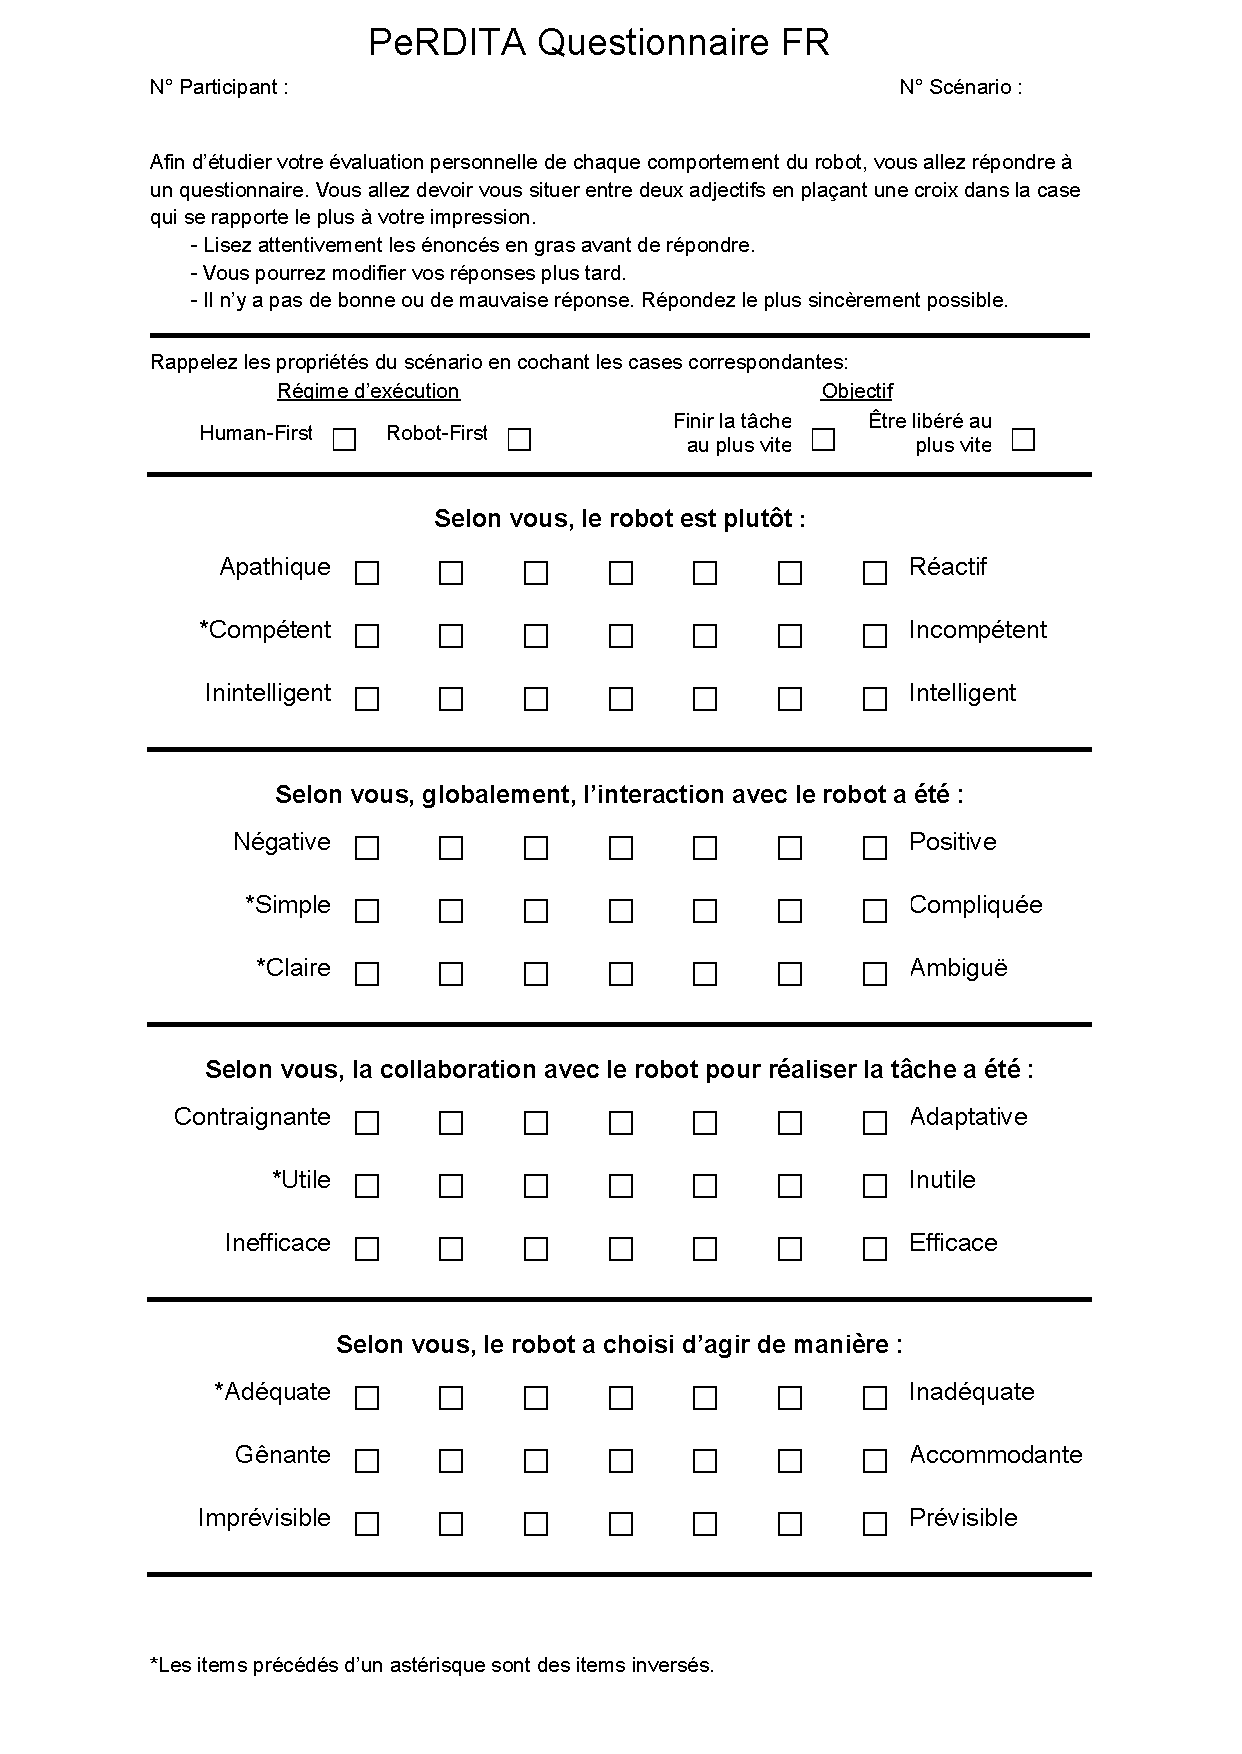
\includepdf[pages=-]{perdita_fr.pdf} %
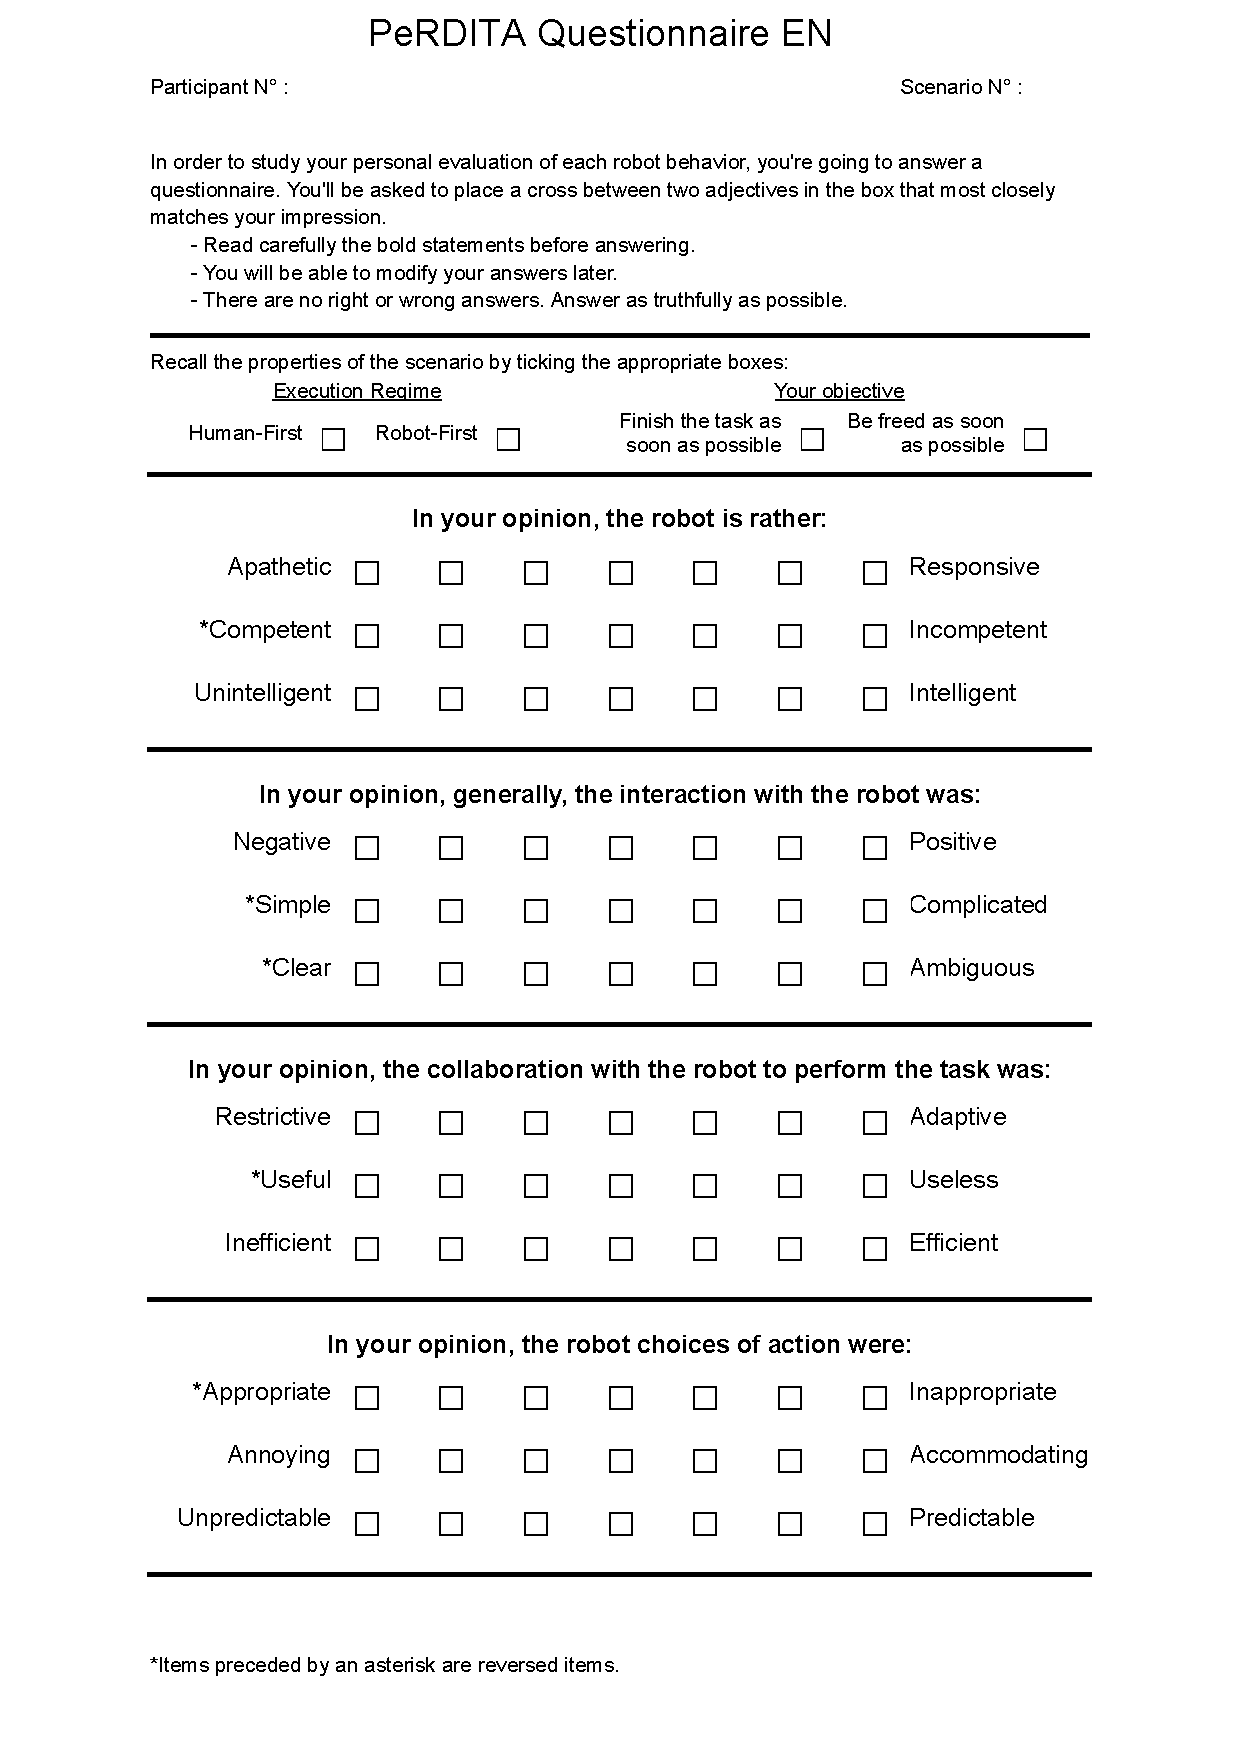
\includepdf[pages=-]{perdita_en.pdf} %

%%%%%%%%%%%%%%%%%%%%%%%%%%%%%%%%%%%%%%%%%%%%%%%%%%%%%%%%%%%%%%%%%%%%%%%%%%%%%%%%%%%%%%%%%%%%%%%%%%%%%%%%%%%%
%%%%%%%%%%%%%%%%%%%%%%%%%%%%%%%%%%%%%%%%%%%%%%%%%%%%%%%%%%%%%%%%%%%%%%%%%%%%%%%%%%%%%%%%%%%%%%%%%%%%%%%%%%%%
%%%%%%%%%%%%%%%%%%%%%%%%%%%%%%%%%%%%%%%%%%%%%%% TABLES %%%%%%%%%%%%%%%%%%%%%%%%%%%%%%%%%%%%%%%%%%%%%%%%%%%%%
%%%%%%%%%%%%%%%%%%%%%%%%%%%%%%%%%%%%%%%%%%%%%%%%%%%%%%%%%%%%%%%%%%%%%%%%%%%%%%%%%%%%%%%%%%%%%%%%%%%%%%%%%%%%
%%%%%%%%%%%%%%%%%%%%%%%%%%%%%%%%%%%%%%%%%%%%%%%%%%%%%%%%%%%%%%%%%%%%%%%%%%%%%%%%%%%%%%%%%%%%%%%%%%%%%%%%%%%%


\begin{sidewaystable}[]
    \center
    \scriptsize
    \begin{tabular}{|c|c|c|c|c|c|c|c|}
    \hline
    \begin{tabular}[c]{@{}c@{}}N°\\ Participant\end{tabular} & Date                                                           & Age & Genre & \begin{tabular}[c]{@{}c@{}}Qu'elle est\\ votre vision \\ de la robotique ?\end{tabular} & \multicolumn{1}{l|}{Affectation} & \begin{tabular}[c]{@{}c@{}}Etes vous familier avec\\ la robotique et la \\ plannification de tâche ?\end{tabular} & \begin{tabular}[c]{@{}c@{}}Avez vous déjà interagi avec un robot ? \\ Si oui quel genre ? \\ (Drone, Robot aspirateur, Humanoïde, Jouet)\end{tabular} \\ \hline
    1                                                        & \begin{tabular}[c]{@{}c@{}}17/12/2023\\ 14:55:45\end{tabular}  & 21  & Male  & 4                                                                                       & EXT                              & Non                                                                                                               & Tous ceux cités                                                                                                                                       \\ \hline
    2                                                        & \begin{tabular}[c]{@{}c@{}}17/12/2023\\ 15:48:14\end{tabular}  & 23  & Woman & 5                                                                                       & EXT                              & Non                                                                                                               & pas vraiment                                                                                                                                          \\ \hline
    3                                                        & \begin{tabular}[c]{@{}c@{}}18/12/2023\\ 10:02:21\end{tabular}  & 26  & Male  & 4                                                                                       & LAAS                             & Oui                                                                                                               & PR2, Pepper                                                                                                                                           \\ \hline
    4                                                        & \begin{tabular}[c]{@{}c@{}}18/12/2023 \\ 10:45:39\end{tabular} & 25  & Male  & 4                                                                                       & LAAS                             & Oui                                                                                                               & thermomix                                                                                                                                             \\ \hline
    5                                                        & \begin{tabular}[c]{@{}c@{}}19/12/2023\\ 10:40:40\end{tabular}  & 28  & Male  & 3                                                                                       & LAAS                             & Oui                                                                                                               & Humanoïde                                                                                                                                             \\ \hline
    6                                                        & \begin{tabular}[c]{@{}c@{}}19/12/2023\\ 11:42:17\end{tabular}  & 26  & Male  & 4                                                                                       & LAAS                             & Non                                                                                                               & Drone                                                                                                                                                 \\ \hline
    7                                                        & \begin{tabular}[c]{@{}c@{}}19/12/2023\\ 14:42:18\end{tabular}  & 26  & Male  & 3                                                                                       & LAAS                             & Non                                                                                                               & Pepper                                                                                                                                                \\ \hline
    8                                                        & \begin{tabular}[c]{@{}c@{}}19/12/2023\\ 15:31:04\end{tabular}  & 24  & Woman & 4                                                                                       & LAAS                             & Non                                                                                                               & robot aspirateur                                                                                                                                      \\ \hline
    9                                                        & \begin{tabular}[c]{@{}c@{}}19/12/2023\\ 19:06:39\end{tabular}  & 26  & Male  & 5                                                                                       & EXT                              & Non                                                                                                               & Robot aspirateur, jouets                                                                                                                              \\ \hline
    10                                                       & \begin{tabular}[c]{@{}c@{}}08/01/2024\\ 10:28:39\end{tabular}  & 30  & Woman & 4                                                                                       & LAAS                             & Oui                                                                                                               & no                                                                                                                                                    \\ \hline
    11                                                       & \begin{tabular}[c]{@{}c@{}}09/01/2024\\ 16:02:02\end{tabular}  & 24  & Male  & 4                                                                                       & LAAS                             & Non                                                                                                               & Pepper, PR2, jouets                                                                                                                                   \\ \hline
    12                                                       & \begin{tabular}[c]{@{}c@{}}09/01/2024\\ 16:32:36\end{tabular}  & 27  & Male  & 5                                                                                       & LAAS                             & Non                                                                                                               & Oui, tous                                                                                                                                             \\ \hline
    13                                                       & \begin{tabular}[c]{@{}c@{}}10/01/2024\\ 16:25:59\end{tabular}  & 27  & Woman & 4                                                                                       & LAAS                             & Non                                                                                                               & \begin{tabular}[c]{@{}c@{}}électroménager +\\  chatbox\end{tabular}                                                                                   \\ \hline
    \end{tabular}
    \caption{Information on the participants. (part~1/2)}
    \label{tab:ap:participant_info_1}
    \end{sidewaystable}

\begin{sidewaystable}[]
    \center
    \scriptsize
    \begin{tabular}{|c|c|c|c|c|c|c|c|}
    \hline
    \begin{tabular}[c]{@{}c@{}}N°\\ Participant\end{tabular} & Date                                                           & Age & Genre & \begin{tabular}[c]{@{}c@{}}Qu'elle est\\ votre vision \\ de la robotique ?\end{tabular} & \multicolumn{1}{l|}{Affectation} & \begin{tabular}[c]{@{}c@{}}Etes vous familier avec\\ la robotique et la \\ plannification de tâche ?\end{tabular} & \begin{tabular}[c]{@{}c@{}}Avez vous déjà interagi avec un robot ? \\ Si oui quel genre ? \\ (Drone, Robot aspirateur, Humanoïde, Jouet)\end{tabular} \\ \hline
    14                                                       & \begin{tabular}[c]{@{}c@{}}11/01/2024\\ 16:00:19\end{tabular}  & 25  & Male  & 5                                                                                       & LAAS                             & Non                                                                                                               & brat manipulateur                                                                                                                                     \\ \hline
    15                                                       & \begin{tabular}[c]{@{}c@{}}12/01/2024\\ 10:11:42\end{tabular}  & 23  & Woman & 5                                                                                       & LAAS                             & Non                                                                                                               & oui (drone, jouet)                                                                                                                                    \\ \hline
    16                                                       & \begin{tabular}[c]{@{}c@{}}12/01/2024\\ 10:56:29\end{tabular}  & 30  & Male  & 4                                                                                       & LAAS                             & Non                                                                                                               & Humanoid                                                                                                                                              \\ \hline
    17                                                       & \begin{tabular}[c]{@{}c@{}}17/01/2024\\ 09:27:52\end{tabular}  & 61  & Male  & 4                                                                                       & LAAS                             & Non                                                                                                               & Oui                                                                                                                                                   \\ \hline
    18                                                       & \begin{tabular}[c]{@{}c@{}}17/01/2024\\ 10:37:37\end{tabular}  & 26  & Male  & 5                                                                                       & LAAS                             & Oui                                                                                                               & \begin{tabular}[c]{@{}c@{}}Drone, Pepper, PR2, \\ Chien robot, \\ Aspirateur,tondeuse, ...\end{tabular}                                               \\ \hline
    19                                                       & \begin{tabular}[c]{@{}c@{}}17/01/2024\\ 17:23:21\end{tabular}  & 27  & Woman & 4                                                                                       & EXT                              & Non                                                                                                               & Non pas vraiment                                                                                                                                      \\ \hline
    20                                                       & \begin{tabular}[c]{@{}c@{}}17/01/2024\\ 17:58:32\end{tabular}  & 29  & Male  & 5                                                                                       & EXT                              & Non                                                                                                               & \begin{tabular}[c]{@{}c@{}}Drone, \\ robot aspirateur\end{tabular}                                                                                    \\ \hline
    21                                                       & \begin{tabular}[c]{@{}c@{}}23/01/2024\\ 10:26:45\end{tabular}  & 25  & Male  & 4                                                                                       & LAAS                             & Oui                                                                                                               & \begin{tabular}[c]{@{}c@{}}Humanoïde, \\ Robot mobile\end{tabular}                                                                                    \\ \hline
    22                                                       & \begin{tabular}[c]{@{}c@{}}23/01/2024\\ 18:03:08\end{tabular}  & 27  & Woman & 4                                                                                       & EXT                              & Non                                                                                                               & Jouet                                                                                                                                                 \\ \hline
    23                                                       & \begin{tabular}[c]{@{}c@{}}25/01/2024\\ 12:15:45\end{tabular}  & 47  & Woman & 4                                                                                       & LAAS                             & Oui                                                                                                               & \begin{tabular}[c]{@{}c@{}}PR2, robot mobile, \\ bras manipulateurs\end{tabular}                                                                      \\ \hline
    24                                                       & \begin{tabular}[c]{@{}c@{}}25/01/2024\\ 13:47:39\end{tabular}  & 26  & Woman & 4                                                                                       & LAAS                             & Non                                                                                                               & PR2 + Jouets                                                                                                                                          \\ \hline
    25                                                       & \begin{tabular}[c]{@{}c@{}}26/01/2024\\ 14:20:54\end{tabular}  & 62  & Male  & 5                                                                                       & LAAS                             & Oui                                                                                                               & \begin{tabular}[c]{@{}c@{}}Bras interactif, \\ humanoïdes, drones\end{tabular}                                                                        \\ \hline
    \end{tabular}
    \caption{Information on the participants. (part~2/2)}
    \label{tab:ap:participant_info_2}
\end{sidewaystable}

\begin{table}[]
    \center
    \footnotesize
    \begin{tabular}{|c|c|c|c|c|c|c|}
    \hline
    \begin{tabular}[c]{@{}c@{}}Participant\\ N°\end{tabular} & \begin{tabular}[c]{@{}c@{}}S1\\ pose\end{tabular} & \begin{tabular}[c]{@{}c@{}}S2\\ pose\end{tabular} & \begin{tabular}[c]{@{}c@{}}S3\\ pose\end{tabular} & \begin{tabular}[c]{@{}c@{}}S4\\ pose\end{tabular} & \begin{tabular}[c]{@{}c@{}}S5\\ pose\end{tabular} & \begin{tabular}[c]{@{}c@{}}S6\\ pose\end{tabular} \\ \hline
    1                                                        & 1                                                 & 2                                                 & 3                                                 & 6                                                 & 5                                                 & 4                                                 \\ \hline
    2                                                        & 3                                                 & 1                                                 & 2                                                 & 6                                                 & 5                                                 & 4                                                 \\ \hline
    3                                                        & 5                                                 & 3                                                 & 6                                                 & 1                                                 & 2                                                 & 4                                                 \\ \hline
    4                                                        & 2                                                 & 5                                                 & 4                                                 & 6                                                 & 3                                                 & 1                                                 \\ \hline
    5                                                        & 1                                                 & 5                                                 & 2                                                 & 6                                                 & 4                                                 & 3                                                 \\ \hline
    6                                                        & 6                                                 & 3                                                 & 4                                                 & 2                                                 & 1                                                 & 5                                                 \\ \hline
    7                                                        & 3                                                 & 5                                                 & 6                                                 & 4                                                 & 1                                                 & 2                                                 \\ \hline
    8                                                        & 4                                                 & 5                                                 & 3                                                 & 6                                                 & 2                                                 & 1                                                 \\ \hline
    9                                                        & 4                                                 & 2                                                 & 1                                                 & 5                                                 & 6                                                 & 3                                                 \\ \hline
    10                                                       & 1                                                 & 5                                                 & 3                                                 & 2                                                 & 4                                                 & 6                                                 \\ \hline
    11                                                       & 5                                                 & 4                                                 & 6                                                 & 2                                                 & 3                                                 & 1                                                 \\ \hline
    12                                                       & 3                                                 & 1                                                 & 5                                                 & 2                                                 & 6                                                 & 4                                                 \\ \hline
    13                                                       & 1                                                 & 2                                                 & 5                                                 & 6                                                 & 4                                                 & 3                                                 \\ \hline
    14                                                       & 4                                                 & 2                                                 & 3                                                 & 1                                                 & 5                                                 & 6                                                 \\ \hline
    15                                                       & 4                                                 & 1                                                 & 6                                                 & 5                                                 & 3                                                 & 2                                                 \\ \hline
    16                                                       & 2                                                 & 6                                                 & 3                                                 & 1                                                 & 4                                                 & 5                                                 \\ \hline
    17                                                       & 2                                                 & 3                                                 & 1                                                 & 5                                                 & 4                                                 & 6                                                 \\ \hline
    18                                                       & 5                                                 & 1                                                 & 3                                                 & 6                                                 & 2                                                 & 4                                                 \\ \hline
    19                                                       & 6                                                 & 1                                                 & 5                                                 & 2                                                 & 4                                                 & 3                                                 \\ \hline
    20                                                       & 4                                                 & 5                                                 & 6                                                 & 3                                                 & 1                                                 & 2                                                 \\ \hline
    21                                                       & 6                                                 & 2                                                 & 4                                                 & 3                                                 & 1                                                 & 5                                                 \\ \hline
    22                                                       & 1                                                 & 4                                                 & 6                                                 & 3                                                 & 2                                                 & 5                                                 \\ \hline
    23                                                       & 2                                                 & 4                                                 & 1                                                 & 3                                                 & 6                                                 & 5                                                 \\ \hline
    24                                                       & 5                                                 & 1                                                 & 4                                                 & 3                                                 & 2                                                 & 6                                                 \\ \hline
    25                                                       & 2                                                 & 1                                                 & 4                                                 & 6                                                 & 3                                                 & 5                                                 \\ \hline
    \end{tabular}
    \caption{Ordering in which each participant encountered each scenario. }
    \label{tab:ap:ordering}
\end{table}

\begin{sidewaystable}[]
    \center
    \scriptsize
    \begin{tabular}{|c|c|c|c|c|c|c|c|c|c|c|c|c|c|c|c|c|c|c|c|c|c|c|c|c|}
    \hline
    N°      & \begin{tabular}[c]{@{}c@{}}S1\\ Q1\end{tabular} & \begin{tabular}[c]{@{}c@{}}S1\\ Q2\end{tabular} & \begin{tabular}[c]{@{}c@{}}S1\\ Q3\end{tabular} & \begin{tabular}[c]{@{}c@{}}S1\\ Q4\end{tabular} & \begin{tabular}[c]{@{}c@{}}S1\\ Q5\end{tabular} & \begin{tabular}[c]{@{}c@{}}S1\\ Q6\end{tabular} & \begin{tabular}[c]{@{}c@{}}S1\\ Q7\end{tabular} & \begin{tabular}[c]{@{}c@{}}S1\\ Q8\end{tabular} & \begin{tabular}[c]{@{}c@{}}S1\\ Q9\end{tabular} & \begin{tabular}[c]{@{}c@{}}S1\\ Q10\end{tabular} & \begin{tabular}[c]{@{}c@{}}S1\\ Q11\end{tabular} & \begin{tabular}[c]{@{}c@{}}S1\\ Q12\end{tabular} & \begin{tabular}[c]{@{}c@{}}S2\\ Q1\end{tabular} & \begin{tabular}[c]{@{}c@{}}S2\\ Q2\end{tabular} & \begin{tabular}[c]{@{}c@{}}S2\\ Q3\end{tabular} & \begin{tabular}[c]{@{}c@{}}S2\\ Q4\end{tabular} & \begin{tabular}[c]{@{}c@{}}S2\\ Q5\end{tabular} & \begin{tabular}[c]{@{}c@{}}S2\\ Q6\end{tabular} & \begin{tabular}[c]{@{}c@{}}S2\\ Q7\end{tabular} & \begin{tabular}[c]{@{}c@{}}S2\\ Q8\end{tabular}   & \begin{tabular}[c]{@{}c@{}}S2\\ Q9\end{tabular} & \begin{tabular}[c]{@{}c@{}}S2\\ Q10\end{tabular} & \begin{tabular}[c]{@{}c@{}}S2\\ Q11\end{tabular} & \begin{tabular}[c]{@{}c@{}}S2\\ Q12\end{tabular} \\ \hline
    1       & 6                                               & 2                                               & 5                                               & 6                                               & 2                                               & 2                                               & 6                                               & 2                                               & 6                                               & 3                                                & 6                                                & 6                                                & 6                                               & 3                                               & 3                                               & 6                                               & 2                                               & 2                                               & 5                                               & 2                                                 & 5                                               & 5                                                & 2                                                & 2                                                \\ \hline
    2       & 6                                               & 1                                               & 7                                               & 7                                               & 1                                               & 1                                               & 7                                               & 1                                               & 7                                               & 1                                                & 7                                                & 7                                                & 7                                               & 1                                               & 7                                               & 7                                               & 1                                               & 1                                               & 7                                               & 1                                                 & 7                                               & 1                                                & 7                                                & 7                                                \\ \hline
    3       & 6                                               & 2                                               & 5                                               & 6                                               & 2                                               & 2                                               & 7                                               & 2                                               & 7                                               & 1                                                & 7                                                & 7                                                & 4                                               & 1                                               & 6                                               & 7                                               & 1                                               & 1                                               & 7                                               & 1                                                 & 7                                               & 1                                                & 7                                                & 3                                                \\ \hline
    4       & 7                                               & 1                                               & 1                                               & 7                                               & 2                                               & 1                                               & 7                                               & 2                                               & 7                                               & 1                                                & 7                                                & 7                                                & 6                                               & 1                                               & 1                                               & 7                                               & 1                                               & 3                                               & 7                                               & 1                                                 & 7                                               & 1                                                & 7                                                & 5                                                \\ \hline
    5       & 6                                               & 3                                               & 3                                               & 6                                               & 3                                               & 3                                               & 6                                               & 3                                               & 6                                               & 2                                                & 5                                                & 6                                                & 6                                               & 2                                               & 5                                               & 6                                               & 3                                               & 3                                               & 6                                               & 3                                                 & 6                                               & 3                                                & 5                                                & 6                                                \\ \hline
    6       & 4                                               & 1                                               & 7                                               & 7                                               & 1                                               & 1                                               & 7                                               & 1                                               & 7                                               & 1                                                & 7                                                & 7                                                & 7                                               & 1                                               & 7                                               & 7                                               & 1                                               & 2                                               & 7                                               & 1                                                 & 7                                               & 1                                                & 7                                                & 6                                                \\ \hline
    7       & 6                                               & 2                                               & 2                                               & 6                                               & 2                                               & 2                                               & 5                                               & 3                                               & 5                                               & 2                                                & 5                                                & 5                                                & 6                                               & 2                                               & 2                                               & 6                                               & 2                                               & 2                                               & 6                                               & 2                                                 & 6                                               & 2                                                & 4                                                & 4                                                \\ \hline
    8       & 7                                               & 1                                               & 7                                               & 7                                               & 1                                               & 1                                               & 7                                               & 1                                               & 7                                               & 1                                                & 7                                                & 7                                                & 7                                               & 2                                               & 7                                               & 7                                               & 3                                               & 2                                               & 6                                               & 3                                                 & 6                                               & 2                                                & 6                                                & 5                                                \\ \hline
    9       & 7                                               & 1                                               & 7                                               & 7                                               & 1                                               & 1                                               & 7                                               & 1                                               & 7                                               & 1                                                & 7                                                & 7                                                & 7                                               & 1                                               & 7                                               & 7                                               & 2                                               & 1                                               & 6                                               & 1                                                 & 7                                               & 1                                                & 7                                                & 7                                                \\ \hline
    10      & 6                                               & 2                                               & 5                                               & 6                                               & 2                                               & 3                                               & 6                                               & 2                                               & 5                                               & 2                                                & 6                                                & 6                                                & 6                                               & 2                                               & 6                                               & 6                                               & 2                                               & 2                                               & 6                                               & 2                                                 & 6                                               & 2                                                & 6                                                & 6                                                \\ \hline
    11      & 7                                               & 1                                               & 7                                               & 7                                               & 1                                               & 1                                               & 7                                               & 1                                               & 7                                               & 1                                                & 7                                                & 7                                                & 7                                               & 1                                               & 7                                               & 7                                               & 1                                               & 1                                               & 7                                               & 1                                                 & 7                                               & 1                                                & 7                                                & 7                                                \\ \hline
    12      & 6                                               & 2                                               & 6                                               & 5                                               & 2                                               & 2                                               & 6                                               & 3                                               & 6                                               & 2                                                & 6                                                & 6                                                & 3                                               & 3                                               & 3                                               & 4                                               & 5                                               & 6                                               & 3                                               & 3                                                 & 2                                               & 5                                                & 3                                                & 4                                                \\ \hline
    13      & 5,5                                             & 6                                               & 4                                               & 6                                               & 1                                               & 1                                               & 6                                               & 3                                               & 5                                               & 2                                                & 7                                                & 7                                                & 7                                               & 1                                               & 4                                               & 7                                               & 1                                               & 1                                               & 7                                               & 2                                                 & 7                                               & 1                                                & 7                                                & 6                                                \\ \hline
    14      & 6                                               & 2                                               & 3                                               & 5                                               & 3                                               & 2                                               & 4                                               & 3                                               & 6                                               & 2                                                & 6                                                & 4                                                & 6                                               & 2                                               & 6                                               & 6                                               & 3                                               & 3                                               & 6                                               & 2                                                 & 6                                               & 3                                                & 6                                                & 5                                                \\ \hline
    15      & 7                                               & 1                                               & 7                                               & 7                                               & 1                                               & 1                                               & 7                                               & 1                                               & 7                                               & 1                                                & 7                                                & 7                                                & 7                                               & 1                                               & 7                                               & 7                                               & 1                                               & 1                                               & 6                                               & 1                                                 & 7                                               & 1                                                & 7                                                & 7                                                \\ \hline
    16      & 6                                               & 3                                               & 6                                               & 6                                               & 2                                               & 2                                               & 7                                               & 6                                               & 6                                               & 2                                                & 6                                                & 6                                                & 6                                               & 2                                               & 6                                               & 6                                               & 2                                               & 2                                               & 7                                               & 2                                                 & 7                                               & 2                                                & 5                                                & 5                                                \\ \hline
    17      & 6                                               & 2                                               & 5                                               & 6                                               & 3                                               & 2                                               & 6                                               & 6                                               & 6                                               & 2                                                & 5                                                & 5                                                & 5                                               & 2                                               & 5                                               & 6                                               & 2                                               & 3                                               & 4                                               & 1                                                 & 6                                               & 2                                                & 4                                                & 6                                                \\ \hline
    18      & 7                                               & 2                                               & 6                                               & 6                                               & 2                                               & 2                                               & 7                                               & 1                                               & 6                                               & 1                                                & 7                                                & 6                                                & 6                                               & 2                                               & 5                                               & 6                                               & 2                                               & 2                                               & 6                                               & 2                                                 & 6                                               & 1                                                & 6                                                & 7                                                \\ \hline
    19      & 6                                               & 1                                               & 7                                               & 6                                               & 1                                               & 1                                               & 7                                               & 1                                               & 7                                               & 1                                                & 7                                                & 7                                                & 7                                               & 1                                               & 6                                               & 6                                               & 4                                               & 4                                               & 6                                               & 2                                                 & 6                                               & 1                                                & 7                                                & 7                                                \\ \hline
    20      & 7                                               & 1                                               & 7                                               & 7                                               & 1                                               & 1                                               & 7                                               & 1                                               & 7                                               & 1                                                & 7                                                & 7                                                & 7                                               & 1                                               & 7                                               & 7                                               & 1                                               & 1                                               & 7                                               & 1                                                 & 7                                               & 1                                                & 7                                                & 6                                                \\ \hline
    21      & 6                                               & 2                                               & 6                                               & 6                                               & 2                                               & 2                                               & 6                                               & 2                                               & 6                                               & 2                                                & 6                                                & 6                                                & 7                                               & 2                                               & 6                                               & 6                                               & 2                                               & 1                                               & 6                                               & 2                                                 & 6                                               & 2                                                & 7                                                & 6                                                \\ \hline
    22      & 7                                               & 1                                               & 4                                               & 7                                               & 1                                               & 1                                               & 7                                               & 1                                               & 7                                               & 1                                                & 7                                                & 7                                                & 7                                               & 2                                               & 4                                               & 6                                               & 2                                               & 2                                               & 5                                               & 1                                                 & 7                                               & 1                                                & 7                                                & 6                                                \\ \hline
    23      & 6                                               & 2                                               & 5                                               & 6                                               & 2                                               & 2                                               & 6                                               & 2                                               & 6                                               & 2                                                & 6                                                & 6                                                & 6                                               & 2                                               & 5                                               & 6                                               & 2                                               & 2                                               & 5                                               & 3                                                 & 5                                               & 2                                                & 6                                                & 6                                                \\ \hline
    24      & 7                                               & 1                                               & 7                                               & 7                                               & 1                                               & 1                                               & 7                                               & 1                                               & 7                                               & 1                                                & 7                                                & 7                                                & 7                                               & 1                                               & 7                                               & 7                                               & 1                                               & 1                                               & 7                                               & 1                                                 & 7                                               & 7                                                & 7                                                & 4                                                \\ \hline
    25      & 6                                               & 2                                               & 6                                               & 5                                               & 2                                               & 2                                               & 6                                               & 2                                               & 6                                               & 2                                                & 6                                                & 6                                                & 6                                               & 2                                               & 6                                               & 5                                               & 2                                               & 2                                               & 3                                               & 2                                                 & 5                                               & 2                                                & 6                                                & 2                                                \\ \hline
    \end{tabular}
    \caption{Participants' answers to the twelve questions of the questionnaire (from Q1 to Q12), for each of the six scenarios (from S1 to S6), on a  - Part 1/3}
    \label{tab:ap:answers_1}
\end{sidewaystable} 

\begin{sidewaystable}[]
    \center
    \scriptsize
    \begin{tabular}{|c|c|c|c|c|c|c|c|c|c|c|c|c|c|c|c|c|c|c|c|c|c|c|c|c|}
    \hline
    N°      & \begin{tabular}[c]{@{}c@{}}S3\\ Q1\end{tabular} & \begin{tabular}[c]{@{}c@{}}S3\\ Q2\end{tabular} & \begin{tabular}[c]{@{}c@{}}S3\\ Q3\end{tabular} & \begin{tabular}[c]{@{}c@{}}S3\\ Q4\end{tabular} & \begin{tabular}[c]{@{}c@{}}S3\\ Q5\end{tabular} & \begin{tabular}[c]{@{}c@{}}S3\\ Q6\end{tabular} & \begin{tabular}[c]{@{}c@{}}S3\\ Q7\end{tabular} & \begin{tabular}[c]{@{}c@{}}S3\\ Q8\end{tabular} & \begin{tabular}[c]{@{}c@{}}S3\\ Q9\end{tabular} & \begin{tabular}[c]{@{}c@{}}S3\\ Q10\end{tabular} & \begin{tabular}[c]{@{}c@{}}S3\\ Q11\end{tabular} & \begin{tabular}[c]{@{}c@{}}S3\\ Q12\end{tabular} & \begin{tabular}[c]{@{}c@{}}S4\\ Q1\end{tabular} & \begin{tabular}[c]{@{}c@{}}S4\\ Q2\end{tabular} & \begin{tabular}[c]{@{}c@{}}S4\\ Q3\end{tabular} & \begin{tabular}[c]{@{}c@{}}S4\\ Q4\end{tabular} & \begin{tabular}[c]{@{}c@{}}S4\\ Q5\end{tabular} & \begin{tabular}[c]{@{}c@{}}S4\\ Q6\end{tabular} & \begin{tabular}[c]{@{}c@{}}S4\\ Q7\end{tabular} & \begin{tabular}[c]{@{}c@{}}S4\\ Q8\end{tabular} & \begin{tabular}[c]{@{}c@{}}S4\\ Q9\end{tabular} & \begin{tabular}[c]{@{}c@{}}S4\\ Q10\end{tabular} & \begin{tabular}[c]{@{}c@{}}S4\\ Q11\end{tabular} & \begin{tabular}[c]{@{}c@{}}S4\\ Q12\end{tabular} \\ \hline
    1       & 6                                               & 3                                               & 3                                               & 6                                               & 2                                               & 2                                               & 5                                               & 2                                               & 5                                               & 5                                                & 2                                                & 2                                                & 6                                               & 2                                               & 6                                               & 6                                               & 2                                               & 2                                               & 6                                               & 1                                               & 6                                               & 2                                                & 6                                                & 5                                                \\ \hline
    2       & 6                                               & 1                                               & 7                                               & 7                                               & 1                                               & 1                                               & 7                                               & 1                                               & 7                                               & 1                                                & 7                                                & 7                                                & 7                                               & 6                                               & 3                                               & 6                                               & 6                                               & 7                                               & 2                                               & 3                                               & 3                                               & 6                                                & 3                                                & 6                                                \\ \hline
    3       & 6                                               & 2                                               & 6                                               & 5                                               & 5                                               & 2                                               & 5                                               & 2                                               & 6                                               & 1                                                & 6                                                & 7                                                & 4                                               & 7                                               & 2                                               & 2                                               & 1                                               & 2                                               & 1                                               & 6                                               & 1                                               & 7                                                & 2                                                & 1                                                \\ \hline
    4       & 7                                               & 1                                               & 1                                               & 6                                               & 1                                               & 1                                               & 7                                               & 1                                               & 7                                               & 2                                                & 7                                                & 7                                                & 7                                               & 7                                               & 1                                               & 3                                               & 1                                               & 1                                               & 3                                               & 2                                               & 4                                               & 6                                                & 3                                                & 7                                                \\ \hline
    5       & 6                                               & 2                                               & 6                                               & 5                                               & 2                                               & 2                                               & 6                                               & 4                                               & 7                                               & 2                                                & 7                                                & 7                                                & 4                                               & 6                                               & 1                                               & 1                                               & 6                                               & 7                                               & 1                                               & 7                                               & 1                                               & 7                                                & 1                                                & 1                                                \\ \hline
    6       & 7                                               & 1                                               & 6                                               & 7                                               & 2                                               & 2                                               & 7                                               & 1                                               & 6                                               & 1                                                & 7                                                & 7                                                & 7                                               & 6                                               & 2                                               & 1                                               & 7                                               & 2                                               & 1                                               & 4                                               & 2                                               & 6                                                & 1                                                & 2                                                \\ \hline
    7       & 4                                               & 2                                               & 6                                               & 6                                               & 2                                               & 2                                               & 4                                               & 5                                               & 6                                               & 2                                                & 6                                                & 6                                                & 6                                               & 2                                               & 6                                               & 2                                               & 6                                               & 6                                               & 2                                               & 6                                               & 2                                               & 6                                                & 2                                                & 6                                                \\ \hline
    8       & 7                                               & 1                                               & 7                                               & 7                                               & 1                                               & 1                                               & 7                                               & 1                                               & 7                                               & 1                                                & 7                                                & 7                                                & 5                                               & 3                                               & 5                                               & 5                                               & 2                                               & 5                                               & 3                                               & 5                                               & 3                                               & 2                                                & 5                                                & 3                                                \\ \hline
    9       & 7                                               & 1                                               & 7                                               & 7                                               & 2                                               & 1                                               & 6                                               & 1                                               & 7                                               & 1                                                & 6                                                & 7                                                & 7                                               & 6                                               & 2                                               & 5                                               & 1                                               & 1                                               & 3                                               & 4                                               & 2                                               & 6                                                & 2                                                & 1                                                \\ \hline
    10      & 5                                               & 3                                               & 5                                               & 6                                               & 2                                               & 3                                               & 5                                               & 3                                               & 5                                               & 5                                                & 4                                                & 4                                                & 3                                               & 5                                               & 3                                               & 3                                               & 2                                               & 4                                               & 3                                               & 4                                               & 2                                               & 6                                                & 2                                                & 4                                                \\ \hline
    11      & 7                                               & 1                                               & 7                                               & 7                                               & 1                                               & 1                                               & 7                                               & 1                                               & 7                                               & 1                                                & 7                                                & 7                                                & 7                                               & 1                                               & 6                                               & 6                                               & 1                                               & 1                                               & 5                                               & 1                                               & 5                                               & 2                                                & 7                                                & 6                                                \\ \hline
    12      & 6                                               & 3                                               & 5                                               & 5                                               & 1                                               & 2                                               & 4                                               & 3                                               & 5                                               & 1                                                & 6                                                & 7                                                & 2                                               & 3                                               & 4                                               & 2                                               & 3                                               & 5                                               & 3                                               & 6                                               & 3                                               & 5                                                & 1                                                & 1                                                \\ \hline
    13      & 7                                               & 1                                               & 6                                               & 7                                               & 1                                               & 1                                               & 7                                               & 2                                               & 7                                               & 1                                                & 7                                                & 7                                                & 7                                               & 2                                               & 3                                               & 6                                               & 1                                               & 1                                               & 3                                               & 4                                               & 5                                               & 5                                                & 6                                                & 3                                                \\ \hline
    14      & 5                                               & 3                                               & 3                                               & 6                                               & 2                                               & 3                                               & 5                                               & 3                                               & 6                                               & 3                                                & 6                                                & 5                                                & 5                                               & 5                                               & 5                                               & 5                                               & 2                                               & 3                                               & 5                                               & 3                                               & 4                                               & 4                                                & 6                                                & 6                                                \\ \hline
    15      & 7                                               & 2                                               & 6                                               & 5                                               & 3                                               & 4                                               & 7                                               & 1                                               & 7                                               & 2                                                & 7                                                & 7                                                & 7                                               & 4                                               & 6                                               & 3                                               & 4                                               & 4                                               & 2                                               & 1                                               & 5                                               & 2                                                & 3                                                & 6                                                \\ \hline
    16      & 6                                               & 3                                               & 6                                               & 6                                               & 2                                               & 2                                               & 7                                               & 6                                               & 6                                               & 2                                                & 6                                                & 6                                                & 5                                               & 5                                               & 5                                               & 5                                               & 3                                               & 3                                               & 4                                               & 4                                               & 3                                               & 5                                                & 3                                                & 3                                                \\ \hline
    17      & 5                                               & 6                                               & 3                                               & 3                                               & 5                                               & 4                                               & 3                                               & 3                                               & 1                                               & 6                                                & 3                                                & 4                                                & 5                                               & 6                                               & 2                                               & 3                                               & 5                                               & 5                                               & 3                                               & 5                                               & 6                                               & 6                                                & 3                                                & 2                                                \\ \hline
    18      & 7                                               & 2                                               & 6                                               & 7                                               & 1                                               & 2                                               & 6                                               & 1                                               & 6                                               & 2                                                & 6                                                & 6                                                & 2                                               & 6                                               & 2                                               & 3                                               & 6                                               & 7                                               & 1                                               & 7                                               & 2                                               & 7                                                & 1                                                & 1                                                \\ \hline
    19      & 7                                               & 1                                               & 7                                               & 7                                               & 1                                               & 1                                               & 7                                               & 1                                               & 7                                               & 1                                                & 7                                                & 7                                                & 6                                               & 7                                               & 1                                               & 1                                               & 7                                               & 5                                               & 1                                               & 7                                               & 2                                               & 7                                                & 1                                                & 1                                                \\ \hline
    20      & 7                                               & 1                                               & 7                                               & 7                                               & 1                                               & 1                                               & 7                                               & 1                                               & 7                                               & 1                                                & 7                                                & 7                                                & 4                                               & 5                                               & 3                                               & 3                                               & 5                                               & 5                                               & 3                                               & 3                                               & 4                                               & 3                                                & 5                                                & 4                                                \\ \hline
    21      & 6                                               & 2                                               & 6                                               & 6                                               & 2                                               & 2                                               & 6                                               & 2                                               & 6                                               & 2                                                & 6                                                & 6                                                & 5                                               & 4                                               & 3                                               & 3                                               & 5                                               & 5                                               & 2                                               & 5                                               & 2                                               & 5                                                & 3                                                & 3                                                \\ \hline
    22      & 7                                               & 1                                               & 4                                               & 7                                               & 1                                               & 1                                               & 7                                               & 1                                               & 7                                               & 1                                                & 7                                                & 7                                                & 7                                               & 6                                               & 3                                               & 1                                               & 6                                               & 7                                               & 2                                               & 6                                               & 3                                               & 7                                                & 1                                                & 1                                                \\ \hline
    23      & 6                                               & 2                                               & 6                                               & 6                                               & 2                                               & 2                                               & 6                                               & 2                                               & 6                                               & 2                                                & 6                                                & 6                                                & 6                                               & 3                                               & 5                                               & 5                                               & 3                                               & 3                                               & 6                                               & 2                                               & 6                                               & 2                                                & 5                                                & 6                                                \\ \hline
    24      & 7                                               & 1                                               & 6                                               & 7                                               & 1                                               & 1                                               & 7                                               & 1                                               & 7                                               & 1                                                & 7                                                & 6                                                & 7                                               & 3                                               & 2                                               & 6                                               & 5                                               & 1                                               & 5                                               & 4                                               & 4                                               & 5                                                & 3                                                & 4                                                \\ \hline
    25      & 6                                               & 2                                               & 2                                               & 7                                               & 2                                               & 2                                               & 6                                               & 2                                               & 6                                               & 2                                                & 6                                                & 7                                                & 6                                               & 6                                               & 2                                               & 2                                               & 3                                               & 4                                               & 2                                               & 3                                               & 2                                               & 6                                                & 2                                                & 3                                                \\ \hline
    \end{tabular}
    \caption{Participants' answers to the 12 questions (Q) of the questionnaire, for each of the 6 scenarios (S) - Part 2/3}
    \label{tab:ap:answers_2}
\end{sidewaystable}

\begin{sidewaystable}[]
    \center
    \scriptsize
    \begin{tabular}{|c|c|c|c|c|c|c|c|c|c|c|c|c|c|c|c|c|c|c|c|c|c|c|c|c|}
    \hline
    N°      & \begin{tabular}[c]{@{}c@{}}S5\\ Q1\end{tabular} & \begin{tabular}[c]{@{}c@{}}S5\\ Q2\end{tabular} & \begin{tabular}[c]{@{}c@{}}S5\\ Q3\end{tabular} & \begin{tabular}[c]{@{}c@{}}S5\\ Q4\end{tabular} & \begin{tabular}[c]{@{}c@{}}S5\\ Q5\end{tabular} & \begin{tabular}[c]{@{}c@{}}S5\\ Q6\end{tabular} & \begin{tabular}[c]{@{}c@{}}S5\\ Q7\end{tabular} & \begin{tabular}[c]{@{}c@{}}S5\\ Q8\end{tabular} & \begin{tabular}[c]{@{}c@{}}S5\\ Q9\end{tabular} & \begin{tabular}[c]{@{}c@{}}S5\\ Q10\end{tabular} & \begin{tabular}[c]{@{}c@{}}S5\\ Q11\end{tabular} & \begin{tabular}[c]{@{}c@{}}S5\\ Q12\end{tabular}  &    \begin{tabular}[c]{@{}c@{}}S6\\ Q1\end{tabular} & \begin{tabular}[c]{@{}c@{}}S6\\ Q2\end{tabular} & \begin{tabular}[c]{@{}c@{}}S6\\ Q3\end{tabular} & \begin{tabular}[c]{@{}c@{}}S6\\ Q4\end{tabular} & \begin{tabular}[c]{@{}c@{}}S6\\ Q5\end{tabular} & \begin{tabular}[c]{@{}c@{}}S6\\ Q6\end{tabular} & \begin{tabular}[c]{@{}c@{}}S6\\ Q7\end{tabular} & \begin{tabular}[c]{@{}c@{}}S6\\ Q8\end{tabular} & \begin{tabular}[c]{@{}c@{}}S6\\ Q9\end{tabular} & \begin{tabular}[c]{@{}c@{}}S6\\ Q10\end{tabular} & \begin{tabular}[c]{@{}c@{}}S6\\ Q11\end{tabular} & \begin{tabular}[c]{@{}c@{}}S6\\ Q12\end{tabular} \\ \hline
    1       & 5                                               & 6                                               & 2                                               & 4                                               & 2                                               & 2                                               & 3                                               & 5                                               & 3                                               & 7                                                & 3                                                & 3                                                 &    6                                               & 3                                               & 2                                               & 5                                               & 2                                               & 2                                               & 3                                               & 6                                               & 3                                               & 6                                                & 1                                                & 1                                                \\ \hline
    2       & 7                                               & 1                                               & 7                                               & 7                                               & 1                                               & 1                                               & 7                                               & 1                                               & 7                                               & 1                                                & 7                                                & 7                                                 &    7                                               & 5                                               & 4                                               & 5                                               & 7                                               & 7                                               & 4                                               & 2                                               & 5                                               & 5                                                & 3                                                & 5                                                \\ \hline
    3       & 6                                               & 2                                               & 4                                               & 6                                               & 2                                               & 1                                               & 5                                               & 3                                               & 7                                               & 1                                                & 7                                                & 7                                                 &    4                                               & 5                                               & 3                                               & 3                                               & 4                                               & 2                                               & 1                                               & 4                                               & 1                                               & 5                                                & 3                                                & 5                                                \\ \hline
    4       & 7                                               & 1                                               & 1                                               & 6                                               & 1                                               & 2                                               & 7                                               & 1                                               & 6                                               & 1                                                & 7                                                & 6                                                 &    7                                               & 5                                               & 1                                               & 5                                               & 1                                               & 2                                               & 3                                               & 4                                               & 6                                               & 4                                                & 6                                                & 7                                                \\ \hline
    5       & 4                                               & 3                                               & 5                                               & 4                                               & 1                                               & 2                                               & 4                                               & 4                                               & 4                                               & 3                                                & 4                                                & 6                                                 &    4                                               & 6                                               & 3                                               & 2                                               & 4                                               & 5                                               & 1                                               & 6                                               & 2                                               & 6                                                & 1                                                & 2                                                \\ \hline
    6       & 7                                               & 1                                               & 7                                               & 7                                               & 1                                               & 2                                               & 7                                               & 1                                               & 7                                               & 1                                                & 7                                                & 6                                                 &    7                                               & 6                                               & 4                                               & 2                                               & 6                                               & 4                                               & 1                                               & 3                                               & 4                                               & 6                                                & 1                                                & 4                                                \\ \hline
    7       & 6                                               & 2                                               & 6                                               & 5                                               & 4                                               & 5                                               & 4                                               & 3                                               & 6                                               & 5                                                & 4                                                & 4                                                 &    6                                               & 2                                               & 6                                               & 2                                               & 6                                               & 6                                               & 3                                               & 3                                               & 5                                               & 5                                                & 2                                                & 2                                                \\ \hline
    8       & 7                                               & 1                                               & 6                                               & 7                                               & 1                                               & 1                                               & 7                                               & 1                                               & 7                                               & 2                                                & 7                                                & 6                                                 &    6                                               & 3                                               & 5                                               & 5                                               & 5                                               & 6                                               & 3                                               & 3                                               & 2                                               & 6                                                & 3                                                & 6                                                \\ \hline
    9       & 7                                               & 1                                               & 6                                               & 7                                               & 1                                               & 2                                               & 7                                               & 1                                               & 6                                               & 2                                                & 7                                                & 6                                                 &    5                                               & 2                                               & 3                                               & 6                                               & 2                                               & 5                                               & 7                                               & 1                                               & 3                                               & 5                                                & 3                                                & 3                                                \\ \hline
    10      & 6                                               & 1                                               & 7                                               & 6                                               & 2                                               & 2                                               & 6                                               & 1                                               & 6                                               & 3                                                & 5                                                & 5                                                 &    4                                               & 5                                               & 2                                               & 3                                               & 2                                               & 4                                               & 2                                               & 5                                               & 2                                               & 5                                                & 2                                                & 4                                                \\ \hline
    11      & 7                                               & 1                                               & 7                                               & 7                                               & 1                                               & 1                                               & 7                                               & 1                                               & 7                                               & 2                                                & 7                                                & 6                                                 &    7                                               & 1                                               & 6                                               & 7                                               & 1                                               & 1                                               & 3                                               & 2                                               & 3                                               & 5                                                & 3                                                & 5                                                \\ \hline
    12      & 5                                               & 3                                               & 2                                               & 3                                               & 1                                               & 5                                               & 7                                               & 2                                               & 5                                               & 4                                                & 3                                                & 5                                                 &    5                                               & 6                                               & 3                                               & 1                                               & 2                                               & 6                                               & 1                                               & 6                                               & 2                                               & 7                                                & 2                                                & 3                                                \\ \hline
    13      & 5                                               & 2                                               & 4                                               & 6                                               & 1                                               & 1                                               & 6                                               & 1                                               & 6                                               & 2                                                & 7                                                & 5                                                 &    5                                               & 4                                               & 4                                               & 5                                               & 1                                               & 1                                               & 5                                               & 4                                               & 5                                               & 5                                                & 4                                                & 5                                                \\ \hline
    14      & 6                                               & 2                                               & 2                                               & 6                                               & 2                                               & 2                                               & 6                                               & 2                                               & 6                                               & 2                                                & 6                                                & 5                                                 &    5                                               & 5                                               & 5                                               & 4                                               & 2                                               & 2                                               & 5                                               & 5                                               & 3                                               & 4                                                & 4                                                & 4                                                \\ \hline
    15      & 7                                               & 2                                               & 5                                               & 6                                               & 3                                               & 4                                               & 7                                               & 2                                               & 6                                               & 3                                                & 7                                                & 4                                                 &    7                                               & 3                                               & 3                                               & 3                                               & 2                                               & 4                                               & 2                                               & 5                                               & 2                                               & 5                                                & 2                                                & 3                                                \\ \hline
    16      & 7                                               & 2                                               & 7                                               & 6                                               & 2                                               & 2                                               & 5                                               & 2                                               & 5                                               & 2                                                & 6                                                & 6                                                 &    4                                               & 4                                               & 4                                               & 5                                               & 3                                               & 4                                               & 4                                               & 3                                               & 3                                               & 5                                                & 3                                                & 5                                                \\ \hline
    17      & 5                                               & 4                                               & 5                                               & 4                                               & 4                                               & 5                                               & 4                                               & 2                                               & 3                                               & 5                                                & 4                                                & 3                                                 &    5                                               & 3                                               & 5                                               & 2                                               & 6                                               & 4                                               & 4                                               & 3                                               & 2                                               & 6                                                & 2                                                & 3                                                \\ \hline
    18      & 6                                               & 3                                               & 6                                               & 7                                               & 3                                               & 3                                               & 6                                               & 1                                               & 6                                               & 3                                                & 6                                                & 7                                                 &    6                                               & 2                                               & 5                                               & 6                                               & 2                                               & 2                                               & 5                                               & 2                                               & 2                                               & 6                                                & 2                                                & 6                                                \\ \hline
    19      & 6                                               & 4                                               & 5                                               & 5                                               & 3                                               & 3                                               & 4                                               & 2                                               & 5                                               & 6                                                & 4                                                & 4                                                 &    5                                               & 2                                               & 5                                               & 4                                               & 4                                               & 5                                               & 5                                               & 2                                               & 6                                               & 4                                                & 2                                                & 6                                                \\ \hline
    20      & 7                                               & 1                                               & 7                                               & 7                                               & 1                                               & 1                                               & 7                                               & 1                                               & 6                                               & 1                                                & 7                                                & 6                                                 &    6                                               & 2                                               & 6                                               & 4                                               & 3                                               & 2                                               & 6                                               & 2                                               & 6                                               & 3                                                & 6                                                & 6                                                \\ \hline
    21      & 6                                               & 2                                               & 6                                               & 6                                               & 2                                               & 2                                               & 6                                               & 2                                               & 6                                               & 2                                                & 6                                                & 6                                                 &    6                                               & 2                                               & 6                                               & 5                                               & 2                                               & 2                                               & 5                                               & 3                                               & 4                                               & 3                                                & 3                                                & 4                                                \\ \hline
    22      & 7                                               & 1                                               & 4                                               & 7                                               & 1                                               & 1                                               & 6                                               & 1                                               & 7                                               & 2                                                & 7                                                & 6                                                 &    7                                               & 7                                               & 1                                               & 1                                               & 7                                               & 7                                               & 1                                               & 7                                               & 1                                               & 7                                                & 1                                                & 1                                                \\ \hline
    23      & 6                                               & 3                                               & 5                                               & 6                                               & 3                                               & 3                                               & 4                                               & 2                                               & 5                                               & 3                                                & 5                                                & 5                                                 &    5                                               & 3                                               & 5                                               & 5                                               & 3                                               & 4                                               & 5                                               & 2                                               & 5                                               & 3                                                & 6                                                & 5                                                \\ \hline
    24      & 7                                               & 2                                               & 5                                               & 7                                               & 1                                               & 1                                               & 7                                               & 1                                               & 6                                               & 2                                                & 7                                                & 6                                                 &    7                                               & 7                                               & 2                                               & 5                                               & 2                                               & 5                                               & 1                                               & 7                                               & 1                                               & 7                                                & 1                                                & 4                                                \\ \hline
    25      & 6                                               & 2                                               & 2                                               & 7                                               & 2                                               & 2                                               & 7                                               & 1                                               & 7                                               & 2                                                & 6                                                & 6                                                 &    6                                               & 2                                               & 2                                               & 2                                               & 4                                               & 3                                               & 2                                               & 3                                               & 2                                               & 6                                                & 2                                                & 2                                                \\ \hline
    \end{tabular}
    \caption{Participants' answers to the 12 questions (Q) of the questionnaire, for each of the 6 scenarios (S) - Part 3/3}
    \label{tab:ap:answers_3}
\end{sidewaystable}

\begin{table}[]
    \center
    \footnotesize
    \begin{tabular}{|c|c|c|c|}
    \hline
    M1  & task\_completion\_time    & M17 & h\_action\_time\_average \\ \hline
    M2  & number\_steps             & M18 & h\_action\_time\_sd      \\ \hline
    M3  & nb\_h\_optimal\_action    & M19 & h\_action\_time\_max     \\ \hline
    M4  & ratio\_h\_optimal\_action & M20 & h\_action\_time\_min     \\ \hline
    M5  & decision\_time\_total     & M21 & r\_action\_nb            \\ \hline
    M6  & decision\_time\_average   & M22 & r\_action\_time\_total   \\ \hline
    M7  & decision\_time\_sd        & M23 & r\_action\_time\_average \\ \hline
    M8  & decision\_time\_max       & M24 & r\_action\_time\_sd      \\ \hline
    M9  & decision\_time\_min       & M25 & r\_action\_time\_max     \\ \hline
    M10 & wait\_ns\_total           & M26 & r\_action\_time\_min     \\ \hline
    M11 & wait\_ns\_average         & M27 & time\_human\_free        \\ \hline
    M12 & wait\_ns\_sd              & M28 & plan\_mvt\_total         \\ \hline
    M13 & wait\_ns\_max             & M29 & plan\_mvt\_min           \\ \hline
    M14 & wait\_ns\_min             & M30 & plan\_mvt\_max           \\ \hline
    M15 & h\_action\_nb             & M31 & plan\_mvt\_average       \\ \hline
    M16 & h\_action\_time\_total    & M32 & plan\_mvt\_sd            \\ \hline
    \end{tabular}
    \caption{Execution metrics abbreviations.}
    \label{tab:ap:metrics_abrv}
\end{table}


\begin{sidewaystable}[]
    \center
    \scriptsize
    \begin{tabular}{|c|c|c|c|c|c|c|c|c|c|c|c|c|c|c|c|c|c|c|c|}
    \hline
    N° & \begin{tabular}[c]{@{}c@{}}S1\\ M1\end{tabular} & \begin{tabular}[c]{@{}c@{}}S1\\ M2\end{tabular} & \begin{tabular}[c]{@{}c@{}}S1\\ M3\end{tabular} & \begin{tabular}[c]{@{}c@{}}S1\\ M4\end{tabular} & \begin{tabular}[c]{@{}c@{}}S1\\ M5\end{tabular} & \begin{tabular}[c]{@{}c@{}}S1\\ M6\end{tabular} & \begin{tabular}[c]{@{}c@{}}S1\\ M7\end{tabular} & \begin{tabular}[c]{@{}c@{}}S1\\ M8\end{tabular} & \begin{tabular}[c]{@{}c@{}}S1\\ M9\end{tabular} & \begin{tabular}[c]{@{}c@{}}S1\\ M10\end{tabular} & \begin{tabular}[c]{@{}c@{}}S1\\ M11\end{tabular} & \begin{tabular}[c]{@{}c@{}}S1\\ M12\end{tabular} & \begin{tabular}[c]{@{}c@{}}S1\\ M13\end{tabular} & \begin{tabular}[c]{@{}c@{}}S1\\ M14\end{tabular} & \begin{tabular}[c]{@{}c@{}}S1\\ M15\end{tabular} & \begin{tabular}[c]{@{}c@{}}S1\\ M16\end{tabular} & \begin{tabular}[c]{@{}c@{}}S1\\ M17\end{tabular} & \begin{tabular}[c]{@{}c@{}}S1\\ M18\end{tabular} & \begin{tabular}[c]{@{}c@{}}S1\\ M19\end{tabular} \\ \hline
    1  & 56,6                                            & 10,0                                            & 10,0                                            & 100,0                                           & 8,2                                             & 1,0                                             & 0,5                                             & 1,8                                             & 0,3                                             & 12,5                                             & 1,6                                              & 0,9                                              & 3,2                                              & 0,6                                              & 8,0                                              & 26,2                                             & 3,3                                              & 0,6                                              & 4,4                                              \\ \hline
    2  & 58,7                                            & 10,0                                            & 10,0                                            & 100,0                                           & 9,7                                             & 1,2                                             & 0,5                                             & 2,0                                             & 0,6                                             & 14,3                                             & 1,8                                              & 1,2                                              & 3,9                                              & 0,7                                              & 8,0                                              & 25,6                                             & 3,2                                              & 0,6                                              & 4,2                                              \\ \hline
    3  & 61,6                                            & 10,0                                            & 9,0                                             & 90,0                                            & 10,3                                            & 1,0                                             & 0,8                                             & 2,9                                             & 0,4                                             & 14,9                                             & 1,9                                              & 1,2                                              & 4,0                                              & 0,7                                              & 8,0                                              & 26,6                                             & 3,3                                              & 0,6                                              & 4,3                                              \\ \hline
    4  & 56,7                                            & 10,0                                            & 9,0                                             & 90,0                                            & 3,8                                             & 0,4                                             & 0,4                                             & 1,2                                             & 0,0                                             & 17,6                                             & 2,2                                              & 1,5                                              & 5,3                                              & 0,6                                              & 8,0                                              & 26,1                                             & 3,3                                              & 0,6                                              & 4,3                                              \\ \hline
    5  & 55,3                                            & 10,0                                            & 10,0                                            & 100,0                                           & 2,9                                             & 0,4                                             & 0,5                                             & 1,2                                             & 0,0                                             & 17,7                                             & 2,2                                              & 1,4                                              & 4,3                                              & 0,6                                              & 8,0                                              & 26,3                                             & 3,3                                              & 0,6                                              & 4,3                                              \\ \hline
    6  & 52,6                                            & 10,0                                            & 10,0                                            & 100,0                                           & 3,6                                             & 0,4                                             & 0,5                                             & 1,7                                             & 0,0                                             & 14,4                                             & 1,8                                              & 1,0                                              & 3,8                                              & 0,7                                              & 8,0                                              & 25,9                                             & 3,2                                              & 0,6                                              & 4,3                                              \\ \hline
    7  & 83,5                                            & 14,0                                            & 10,0                                            & 71,4                                            & 12,0                                            & 0,9                                             & 0,7                                             & 2,4                                             & 0,1                                             & 11,8                                             & 2,0                                              & 1,1                                              & 4,0                                              & 0,6                                              & 6,0                                              & 18,7                                             & 3,1                                              & 0,5                                              & 4,2                                              \\ \hline
    8  & 60,6                                            & 10,0                                            & 9,0                                             & 90,0                                            & 2,8                                             & 0,3                                             & 0,6                                             & 1,9                                             & 0,0                                             & 14,5                                             & 1,8                                              & 1,2                                              & 4,2                                              & 0,7                                              & 8,0                                              & 26,4                                             & 3,3                                              & 0,6                                              & 4,3                                              \\ \hline
    9  & 61,3                                            & 10,0                                            & 10,0                                            & 100,0                                           & 7,3                                             & 0,9                                             & 0,5                                             & 2,0                                             & 0,6                                             & 18,3                                             & 2,3                                              & 1,3                                              & 4,3                                              & 0,7                                              & 8,0                                              & 25,9                                             & 3,2                                              & 0,6                                              & 4,3                                              \\ \hline
    10 & 62,4                                            & 10,0                                            & 10,0                                            & 100,0                                           & 14,1                                            & 1,8                                             & 2,3                                             & 6,8                                             & 0,0                                             & 13,9                                             & 1,7                                              & 1,0                                              & 3,6                                              & 0,7                                              & 8,0                                              & 26,0                                             & 3,3                                              & 0,6                                              & 4,3                                              \\ \hline
    11 & 58,6                                            & 10,0                                            & 10,0                                            & 100,0                                           & 4,6                                             & 0,5                                             & 0,5                                             & 1,8                                             & 0,1                                             & 20,2                                             & 2,5                                              & 1,8                                              & 6,5                                              & 0,6                                              & 8,0                                              & 25,8                                             & 3,2                                              & 0,6                                              & 4,3                                              \\ \hline
    12 & 58,3                                            & 10,0                                            & 10,0                                            & 100,0                                           & 3,6                                             & 0,5                                             & 1,0                                             & 3,2                                             & 0,0                                             & 18,9                                             & 2,4                                              & 1,7                                              & 5,7                                              & 0,7                                              & 8,0                                              & 26,2                                             & 3,3                                              & 0,6                                              & 4,3                                              \\ \hline
    13 & 61,4                                            & 12,0                                            & 10,0                                            & 83,3                                            & 1,6                                             & 0,1                                             & 0,2                                             & 0,4                                             & 0,0                                             & 17,9                                             & 1,8                                              & 1,1                                              & 4,1                                              & 0,7                                              & 10,0                                             & 32,7                                             & 3,3                                              & 0,6                                              & 4,3                                              \\ \hline
    14 & 57,5                                            & 10,0                                            & 10,0                                            & 100,0                                           & 3,5                                             & 0,4                                             & 0,6                                             & 1,7                                             & 0,0                                             & 20,7                                             & 2,6                                              & 1,8                                              & 6,8                                              & 0,6                                              & 8,0                                              & 26,0                                             & 3,2                                              & 0,6                                              & 4,3                                              \\ \hline
    15 & 62,3                                            & 10,0                                            & 9,0                                             & 90,0                                            & 2,7                                             & 0,3                                             & 0,6                                             & 1,9                                             & 0,0                                             & 18,3                                             & 2,3                                              & 1,5                                              & 4,8                                              & 0,6                                              & 8,0                                              & 26,4                                             & 3,3                                              & 0,6                                              & 4,3                                              \\ \hline
    16 & 60,2                                            & 10,0                                            & 10,0                                            & 100,0                                           & 4,5                                             & 0,6                                             & 1,0                                             & 3,1                                             & 0,0                                             & 19,4                                             & 2,4                                              & 1,5                                              & 4,7                                              & 0,6                                              & 8,0                                              & 25,9                                             & 3,2                                              & 0,6                                              & 4,3                                              \\ \hline
    17 & 59,3                                            & 10,0                                            & 10,0                                            & 100,0                                           & 10,2                                            & 1,3                                             & 1,8                                             & 5,8                                             & 0,0                                             & 13,0                                             & 1,6                                              & 0,9                                              & 3,0                                              & 0,6                                              & 8,0                                              & 25,8                                             & 3,2                                              & 0,6                                              & 4,2                                              \\ \hline
    18 & 56,5                                            & 10,0                                            & 10,0                                            & 100,0                                           & 2,7                                             & 0,3                                             & 0,2                                             & 0,8                                             & 0,0                                             & 18,9                                             & 2,4                                              & 1,7                                              & 5,6                                              & 0,6                                              & 8,0                                              & 26,1                                             & 3,3                                              & 0,6                                              & 4,3                                              \\ \hline
    19 & 59,7                                            & 10,0                                            & 9,0                                             & 90,0                                            & 4,9                                             & 0,5                                             & 1,0                                             & 3,0                                             & 0,0                                             & 14,2                                             & 1,8                                              & 1,5                                              & 5,1                                              & 0,6                                              & 8,0                                              & 26,6                                             & 3,3                                              & 0,6                                              & 4,3                                              \\ \hline
    20 & 54,8                                            & 10,0                                            & 10,0                                            & 100,0                                           & 2,8                                             & 0,3                                             & 0,2                                             & 0,7                                             & 0,0                                             & 17,2                                             & 2,2                                              & 1,7                                              & 5,1                                              & 0,6                                              & 8,0                                              & 26,2                                             & 3,3                                              & 0,6                                              & 4,4                                              \\ \hline
    21 & 55,2                                            & 10,0                                            & 10,0                                            & 100,0                                           & 1,6                                             & 0,2                                             & 0,2                                             & 0,5                                             & 0,0                                             & 18,6                                             & 2,3                                              & 1,4                                              & 4,9                                              & 0,6                                              & 8,0                                              & 25,8                                             & 3,2                                              & 0,6                                              & 4,3                                              \\ \hline
    22 & 60,3                                            & 10,0                                            & 10,0                                            & 100,0                                           & 8,7                                             & 1,1                                             & 0,5                                             & 1,9                                             & 0,5                                             & 16,1                                             & 2,0                                              & 1,0                                              & 4,0                                              & 0,6                                              & 8,0                                              & 26,1                                             & 3,3                                              & 0,6                                              & 4,3                                              \\ \hline
    23 & 67,4                                            & 12,0                                            & 10,0                                            & 83,3                                            & 6,8                                             & 0,7                                             & 1,1                                             & 3,5                                             & 0,0                                             & 19,5                                             & 2,0                                              & 1,4                                              & 4,6                                              & 0,7                                              & 10,0                                             & 32,6                                             & 3,3                                              & 0,6                                              & 4,3                                              \\ \hline
    24 & 56,5                                            & 10,0                                            & 10,0                                            & 100,0                                           & 9,8                                             & 1,1                                             & 0,5                                             & 2,0                                             & 0,4                                             & 11,6                                             & 1,5                                              & 0,7                                              & 2,5                                              & 0,7                                              & 8,0                                              & 26,0                                             & 3,3                                              & 0,6                                              & 4,3                                              \\ \hline
    25 & 58,5                                            & 10,0                                            & 10,0                                            & 100,0                                           & 2,7                                             & 0,3                                             & 0,5                                             & 1,8                                             & 0,0                                             & 18,9                                             & 2,4                                              & 1,4                                              & 5,0                                              & 0,6                                              & 8,0                                              & 25,8                                             & 3,2                                              & 0,6                                              & 4,2                                              \\ \hline
    \end{tabular}
    \caption{Execution metrics - Part 1/10}
    \label{tab:ap:exec_metrics_1}
\end{sidewaystable}

\begin{sidewaystable}[]
    \center
    \scriptsize
    \begin{tabular}{|c|c|c|c|c|c|c|c|c|c|c|c|c|c|c|c|c|c|c|c|}
    \hline
    N° & \begin{tabular}[c]{@{}c@{}}S1\\ M20\end{tabular} & \begin{tabular}[c]{@{}c@{}}S1\\ M21\end{tabular} & \begin{tabular}[c]{@{}c@{}}S1\\ M22\end{tabular} & \begin{tabular}[c]{@{}c@{}}S1\\ M23\end{tabular} & \begin{tabular}[c]{@{}c@{}}S1\\ M24\end{tabular} & \begin{tabular}[c]{@{}c@{}}S1\\ M25\end{tabular} & \begin{tabular}[c]{@{}c@{}}S1\\ M26\end{tabular} & \begin{tabular}[c]{@{}c@{}}S1\\ M27\end{tabular} & \begin{tabular}[c]{@{}c@{}}S1\\ M28\end{tabular} & \begin{tabular}[c]{@{}c@{}}S1\\ M29\end{tabular} & \begin{tabular}[c]{@{}c@{}}S1\\ M30\end{tabular} & \begin{tabular}[c]{@{}c@{}}S1\\ M31\end{tabular} & \begin{tabular}[c]{@{}c@{}}S1\\ M32\end{tabular} & \begin{tabular}[c]{@{}c@{}}S2\\ M1\end{tabular} & \begin{tabular}[c]{@{}c@{}}S2\\ M2\end{tabular} & \begin{tabular}[c]{@{}c@{}}S2\\ M3\end{tabular} & \begin{tabular}[c]{@{}c@{}}S2\\ M4\end{tabular} & \begin{tabular}[c]{@{}c@{}}S2\\ M5\end{tabular} & \begin{tabular}[c]{@{}c@{}}S2\\ M6\end{tabular} \\ \hline
    1  & 2,6                                              & 8,0                                              & 28,2                                             & 3,5                                              & 0,6                                              & 4,5                                              & 2,6                                              & 22,1                                             & 5,7                                              & 0,0                                              & 1,2                                              & 0,6                                              & 0,3                                              & 59,5                                            & 10,0                                            & 10,0                                            & 100,0                                           & 18,3                                            & 2,3                                             \\ \hline
    2  & 2,5                                              & 8,0                                              & 31,3                                             & 3,9                                              & 0,9                                              & 5,8                                              & 2,7                                              & 22,7                                             & 3,2                                              & 0,0                                              & 0,7                                              & 0,3                                              & 0,2                                              & 54,7                                            & 10,0                                            & 10,0                                            & 100,0                                           & 7,8                                             & 1,0                                             \\ \hline
    3  & 2,6                                              & 8,0                                              & 29,8                                             & 3,7                                              & 0,9                                              & 6,1                                              & 3,0                                              & 61,6                                             & 5,8                                              & 0,1                                              & 1,8                                              & 0,7                                              & 0,4                                              & 53,9                                            & 10,0                                            & 10,0                                            & 100,0                                           & 11,0                                            & 1,4                                             \\ \hline
    4  & 2,5                                              & 8,0                                              & 33,4                                             & 4,2                                              & 1,2                                              & 7,0                                              & 2,9                                              & 56,7                                             & 4,1                                              & 0,2                                              & 0,7                                              & 0,5                                              & 0,2                                              & 50,0                                            & 10,0                                            & 10,0                                            & 100,0                                           & 3,8                                             & 0,4                                             \\ \hline
    5  & 2,7                                              & 8,0                                              & 34,0                                             & 4,2                                              & 1,4                                              & 6,7                                              & 3,1                                              & 18,8                                             & 3,9                                              & 0,0                                              & 0,7                                              & 0,4                                              & 0,3                                              & 51,1                                            & 10,0                                            & 10,0                                            & 100,0                                           & 1,6                                             & 0,2                                             \\ \hline
    6  & 2,7                                              & 8,0                                              & 28,8                                             & 3,6                                              & 0,8                                              & 5,2                                              & 2,8                                              & 18,2                                             & 5,5                                              & 0,0                                              & 0,8                                              & 0,6                                              & 0,3                                              & 50,0                                            & 10,0                                            & 10,0                                            & 100,0                                           & 2,0                                             & 0,3                                             \\ \hline
    7  & 2,6                                              & 12,0                                             & 53,2                                             & 4,4                                              & 1,5                                              & 7,9                                              & 3,1                                              & 21,0                                             & 6,1                                              & 0,0                                              & 0,7                                              & 0,4                                              & 0,3                                              & 54,4                                            & 10,0                                            & 10,0                                            & 100,0                                           & 6,5                                             & 0,8                                             \\ \hline
    8  & 2,6                                              & 8,0                                              & 32,5                                             & 4,1                                              & 1,2                                              & 5,8                                              & 2,7                                              & 60,6                                             & 5,0                                              & 0,3                                              & 1,0                                              & 0,6                                              & 0,2                                              & 59,4                                            & 11,0                                            & 10,0                                            & 90,9                                            & 6,2                                             & 0,8                                             \\ \hline
    9  & 2,6                                              & 8,0                                              & 35,4                                             & 4,4                                              & 1,0                                              & 5,9                                              & 3,0                                              & 22,9                                             & 4,2                                              & 0,0                                              & 0,8                                              & 0,4                                              & 0,3                                              & 52,7                                            & 10,0                                            & 10,0                                            & 100,0                                           & 3,8                                             & 0,5                                             \\ \hline
    10 & 2,6                                              & 8,0                                              & 30,6                                             & 3,8                                              & 0,8                                              & 5,0                                              & 2,6                                              & 25,2                                             & 4,5                                              & 0,0                                              & 0,7                                              & 0,5                                              & 0,3                                              & 64,0                                            & 12,0                                            & 10,0                                            & 83,3                                            & 17,1                                            & 2,1                                             \\ \hline
    11 & 2,6                                              & 8,0                                              & 34,6                                             & 4,3                                              & 1,3                                              & 6,9                                              & 3,1                                              & 22,5                                             & 5,4                                              & 0,0                                              & 1,1                                              & 0,5                                              & 0,3                                              & 53,1                                            & 10,0                                            & 10,0                                            & 100,0                                           & 9,7                                             & 1,2                                             \\ \hline
    12 & 2,6                                              & 8,0                                              & 35,3                                             & 4,4                                              & 1,2                                              & 6,2                                              & 3,0                                              & 21,0                                             & 4,9                                              & 0,0                                              & 1,2                                              & 0,5                                              & 0,4                                              & 54,5                                            & 10,0                                            & 10,0                                            & 100,0                                           & 12,3                                            & 1,5                                             \\ \hline
    13 & 2,6                                              & 8,0                                              & 32,2                                             & 4,0                                              & 0,8                                              & 5,6                                              & 3,3                                              & 17,5                                             & 4,9                                              & 0,0                                              & 0,8                                              & 0,4                                              & 0,3                                              & 57,0                                            & 10,0                                            & 10,0                                            & 100,0                                           & 8,2                                             & 1,0                                             \\ \hline
    14 & 2,7                                              & 8,0                                              & 34,4                                             & 4,3                                              & 1,2                                              & 6,2                                              & 3,0                                              & 24,4                                             & 5,0                                              & 0,0                                              & 2,3                                              & 0,5                                              & 0,6                                              & 63,0                                            & 11,0                                            & 10,0                                            & 90,9                                            & 12,7                                            & 1,6                                             \\ \hline
    15 & 2,7                                              & 8,0                                              & 33,9                                             & 4,2                                              & 1,2                                              & 6,5                                              & 3,0                                              & 62,3                                             & 5,2                                              & 0,5                                              & 0,8                                              & 0,6                                              & 0,1                                              & 58,3                                            & 10,0                                            & 10,0                                            & 100,0                                           & 12,0                                            & 1,5                                             \\ \hline
    16 & 2,6                                              & 8,0                                              & 36,2                                             & 4,5                                              & 1,2                                              & 6,2                                              & 2,8                                              & 19,8                                             & 5,0                                              & 0,0                                              & 0,7                                              & 0,5                                              & 0,3                                              & 60,9                                            & 11,0                                            & 10,0                                            & 90,9                                            & 11,3                                            & 1,4                                             \\ \hline
    17 & 2,6                                              & 8,0                                              & 30,6                                             & 3,8                                              & 1,1                                              & 5,5                                              & 2,3                                              & 19,2                                             & 3,7                                              & 0,0                                              & 0,7                                              & 0,4                                              & 0,3                                              & 75,8                                            & 14,0                                            & 10,0                                            & 71,4                                            & 5,4                                             & 0,9                                             \\ \hline
    18 & 2,6                                              & 8,0                                              & 34,3                                             & 4,3                                              & 1,5                                              & 7,4                                              & 3,1                                              & 18,4                                             & 5,0                                              & 0,0                                              & 0,8                                              & 0,5                                              & 0,3                                              & 52,3                                            & 10,0                                            & 10,0                                            & 100,0                                           & 5,8                                             & 0,6                                             \\ \hline
    19 & 2,6                                              & 8,0                                              & 29,9                                             & 3,7                                              & 1,2                                              & 6,7                                              & 2,9                                              & 59,7                                             & 4,3                                              & 0,1                                              & 0,7                                              & 0,5                                              & 0,2                                              & 54,0                                            & 11,0                                            & 10,0                                            & 90,9                                            & 0,9                                             & 0,1                                             \\ \hline
    20 & 2,7                                              & 8,0                                              & 33,0                                             & 4,1                                              & 1,3                                              & 6,7                                              & 3,1                                              & 20,3                                             & 4,4                                              & 0,0                                              & 0,8                                              & 0,4                                              & 0,3                                              & 56,7                                            & 10,0                                            & 10,0                                            & 100,0                                           & 10,9                                            & 1,4                                             \\ \hline
    21 & 2,6                                              & 8,0                                              & 33,9                                             & 4,2                                              & 1,0                                              & 6,0                                              & 2,7                                              & 20,5                                             & 5,0                                              & 0,0                                              & 0,9                                              & 0,5                                              & 0,3                                              & 44,7                                            & 10,0                                            & 10,0                                            & 100,0                                           & 1,7                                             & 0,2                                             \\ \hline
    22 & 2,7                                              & 8,0                                              & 31,3                                             & 3,9                                              & 0,9                                              & 5,8                                              & 2,8                                              & 23,2                                             & 5,7                                              & 0,0                                              & 0,9                                              & 0,6                                              & 0,3                                              & 51,8                                            & 10,0                                            & 10,0                                            & 100,0                                           & 9,0                                             & 1,1                                             \\ \hline
    23 & 2,6                                              & 8,0                                              & 32,2                                             & 4,0                                              & 0,9                                              & 5,4                                              & 3,1                                              & 24,5                                             & 5,3                                              & 0,0                                              & 0,7                                              & 0,4                                              & 0,3                                              & 64,6                                            & 12,0                                            & 10,0                                            & 83,3                                            & 6,9                                             & 1,0                                             \\ \hline
    24 & 2,6                                              & 8,0                                              & 28,3                                             & 3,5                                              & 0,4                                              & 4,1                                              & 2,8                                              & 20,9                                             & 4,1                                              & 0,0                                              & 0,7                                              & 0,4                                              & 0,3                                              & 54,2                                            & 10,0                                            & 10,0                                            & 100,0                                           & 10,2                                            & 1,3                                             \\ \hline
    25 & 2,6                                              & 8,0                                              & 36,5                                             & 4,6                                              & 1,3                                              & 6,6                                              & 2,7                                              & 19,9                                             & 4,6                                              & 0,0                                              & 0,9                                              & 0,5                                              & 0,3                                              & 65,2                                            & 12,0                                            & 10,0                                            & 83,3                                            & 11,5                                            & 1,4                                             \\ \hline
    \end{tabular}
    \caption{Execution metrics - Part 2/10}
    \label{tab:ap:exec_metrics_2}
\end{sidewaystable}


\begin{sidewaystable}[]
    \center
    \scriptsize
    \begin{tabular}{|c|c|c|c|c|c|c|c|c|c|c|c|c|c|c|c|c|c|c|c|}
    \hline
    N° & \begin{tabular}[c]{@{}c@{}}S2\\ M7\end{tabular} & \begin{tabular}[c]{@{}c@{}}S2\\ M8\end{tabular} & \begin{tabular}[c]{@{}c@{}}S2\\ M9\end{tabular} & \begin{tabular}[c]{@{}c@{}}S2\\ M10\end{tabular} & \begin{tabular}[c]{@{}c@{}}S2\\ M11\end{tabular} & \begin{tabular}[c]{@{}c@{}}S2\\ M12\end{tabular} & \begin{tabular}[c]{@{}c@{}}S2\\ M13\end{tabular} & \begin{tabular}[c]{@{}c@{}}S2\\ M14\end{tabular} & \begin{tabular}[c]{@{}c@{}}S2\\ M15\end{tabular} & \begin{tabular}[c]{@{}c@{}}S2\\ M16\end{tabular} & \begin{tabular}[c]{@{}c@{}}S2\\ M17\end{tabular} & \begin{tabular}[c]{@{}c@{}}S2\\ M18\end{tabular} & \begin{tabular}[c]{@{}c@{}}S2\\ M19\end{tabular} & \begin{tabular}[c]{@{}c@{}}S2\\ M20\end{tabular} & \begin{tabular}[c]{@{}c@{}}S2\\ M21\end{tabular} & \begin{tabular}[c]{@{}c@{}}S2\\ M22\end{tabular} & \begin{tabular}[c]{@{}c@{}}S2\\ M23\end{tabular} & \begin{tabular}[c]{@{}c@{}}S2\\ M24\end{tabular} & \begin{tabular}[c]{@{}c@{}}S2\\ M25\end{tabular} \\ \hline
    1  & 1,4                                             & 5,4                                             & 0,9                                             & 5,9                                              & 0,7                                              & 0,1                                              & 1,1                                              & 0,6                                              & 8,0                                              & 26,0                                             & 3,3                                              & 0,6                                              & 4,3                                              & 2,6                                              & 8,0                                              & 31,2                                             & 3,9                                              & 0,9                                              & 5,9                                              \\ \hline
    2  & 0,4                                             & 1,9                                             & 0,4                                             & 8,3                                              & 1,0                                              & 0,4                                              & 1,6                                              & 0,6                                              & 8,0                                              & 26,1                                             & 3,3                                              & 0,6                                              & 4,3                                              & 2,6                                              & 8,0                                              & 31,2                                             & 3,9                                              & 0,6                                              & 4,9                                              \\ \hline
    3  & 0,8                                             & 2,8                                             & 0,2                                             & 8,3                                              & 1,0                                              & 0,5                                              & 2,0                                              & 0,6                                              & 8,0                                              & 26,2                                             & 3,3                                              & 0,6                                              & 4,3                                              & 2,6                                              & 8,0                                              & 30,3                                             & 3,8                                              & 0,8                                              & 5,3                                              \\ \hline
    4  & 0,5                                             & 1,5                                             & 0,0                                             & 11,7                                             & 1,5                                              & 1,1                                              & 3,6                                              & 0,6                                              & 8,0                                              & 26,2                                             & 3,3                                              & 0,6                                              & 4,2                                              & 2,6                                              & 8,0                                              & 30,1                                             & 3,8                                              & 1,2                                              & 6,7                                              \\ \hline
    5  & 0,2                                             & 0,6                                             & 0,0                                             & 14,8                                             & 1,8                                              & 1,5                                              & 5,3                                              & 0,6                                              & 8,0                                              & 26,3                                             & 3,3                                              & 0,6                                              & 4,3                                              & 2,7                                              & 8,0                                              & 32,1                                             & 4,0                                              & 1,2                                              & 6,9                                              \\ \hline
    6  & 0,2                                             & 0,6                                             & 0,0                                             & 12,9                                             & 1,6                                              & 1,2                                              & 4,3                                              & 0,7                                              & 8,0                                              & 26,1                                             & 3,3                                              & 0,6                                              & 4,3                                              & 2,6                                              & 8,0                                              & 32,6                                             & 4,1                                              & 0,9                                              & 5,7                                              \\ \hline
    7  & 1,5                                             & 4,7                                             & 0,0                                             & 10,8                                             & 1,4                                              & 1,0                                              & 3,8                                              & 0,6                                              & 8,0                                              & 26,3                                             & 3,3                                              & 0,6                                              & 4,3                                              & 2,6                                              & 8,0                                              & 31,9                                             & 4,0                                              & 0,9                                              & 5,8                                              \\ \hline
    8  & 1,2                                             & 3,8                                             & 0,0                                             & 12,4                                             & 1,6                                              & 1,5                                              & 4,8                                              & 0,6                                              & 8,0                                              & 26,3                                             & 3,3                                              & 0,6                                              & 4,3                                              & 2,7                                              & 8,0                                              & 35,4                                             & 4,4                                              & 1,2                                              & 6,4                                              \\ \hline
    9  & 0,5                                             & 1,6                                             & 0,0                                             & 11,1                                             & 1,4                                              & 0,8                                              & 2,5                                              & 0,6                                              & 8,0                                              & 26,2                                             & 3,3                                              & 0,6                                              & 4,3                                              & 2,6                                              & 8,0                                              & 33,0                                             & 4,1                                              & 1,2                                              & 6,3                                              \\ \hline
    10 & 1,9                                             & 5,9                                             & 0,0                                             & 8,2                                              & 1,0                                              & 0,6                                              & 2,4                                              & 0,6                                              & 8,0                                              & 26,1                                             & 3,3                                              & 0,6                                              & 4,3                                              & 2,6                                              & 8,0                                              & 30,2                                             & 3,8                                              & 1,1                                              & 5,9                                              \\ \hline
    11 & 0,9                                             & 2,9                                             & 0,0                                             & 9,7                                              & 1,2                                              & 0,8                                              & 2,6                                              & 0,6                                              & 8,0                                              & 25,9                                             & 3,2                                              & 0,6                                              & 4,3                                              & 2,6                                              & 8,0                                              & 30,0                                             & 3,8                                              & 1,1                                              & 6,3                                              \\ \hline
    12 & 1,1                                             & 3,9                                             & 0,0                                             & 6,2                                              & 0,8                                              & 0,2                                              & 1,2                                              & 0,6                                              & 8,0                                              & 26,1                                             & 3,3                                              & 0,7                                              & 4,4                                              & 2,6                                              & 8,0                                              & 30,9                                             & 3,9                                              & 0,8                                              & 5,4                                              \\ \hline
    13 & 1,2                                             & 3,7                                             & 0,0                                             & 14,4                                             & 1,8                                              & 1,3                                              & 4,7                                              & 0,6                                              & 8,0                                              & 26,0                                             & 3,3                                              & 0,6                                              & 4,3                                              & 2,6                                              & 8,0                                              & 34,8                                             & 4,3                                              & 2,0                                              & 8,7                                              \\ \hline
    14 & 1,9                                             & 4,8                                             & 0,0                                             & 9,7                                              & 1,2                                              & 0,6                                              & 2,4                                              & 0,6                                              & 8,0                                              & 26,0                                             & 3,3                                              & 0,6                                              & 4,4                                              & 2,6                                              & 8,0                                              & 31,4                                             & 3,9                                              & 0,6                                              & 4,8                                              \\ \hline
    15 & 1,5                                             & 4,7                                             & 0,0                                             & 12,2                                             & 1,5                                              & 1,6                                              & 5,6                                              & 0,6                                              & 8,0                                              & 26,0                                             & 3,2                                              & 0,6                                              & 4,3                                              & 2,7                                              & 8,0                                              & 34,5                                             & 4,3                                              & 1,2                                              & 6,3                                              \\ \hline
    16 & 1,3                                             & 3,5                                             & 0,0                                             & 7,6                                              & 0,9                                              & 0,7                                              & 2,8                                              & 0,6                                              & 8,0                                              & 26,3                                             & 3,3                                              & 0,7                                              & 4,4                                              & 2,7                                              & 8,0                                              & 34,3                                             & 4,3                                              & 1,1                                              & 6,2                                              \\ \hline
    17 & 1,8                                             & 5,0                                             & 0,0                                             & 13,7                                             & 2,3                                              & 1,0                                              & 3,6                                              & 0,7                                              & 6,0                                              & 19,7                                             & 3,3                                              & 0,7                                              & 4,3                                              & 2,6                                              & 12,0                                             & 48,6                                             & 4,1                                              & 1,0                                              & 6,0                                              \\ \hline
    18 & 0,8                                             & 2,5                                             & 0,0                                             & 11,5                                             & 1,4                                              & 0,9                                              & 3,3                                              & 0,6                                              & 8,0                                              & 26,5                                             & 3,3                                              & 0,6                                              & 4,4                                              & 2,6                                              & 8,0                                              & 31,1                                             & 3,9                                              & 0,7                                              & 4,7                                              \\ \hline
    19 & 0,2                                             & 0,6                                             & 0,0                                             & 8,9                                              & 1,1                                              & 0,6                                              & 2,2                                              & 0,6                                              & 8,0                                              & 26,3                                             & 3,3                                              & 0,6                                              & 4,3                                              & 2,6                                              & 8,0                                              & 28,1                                             & 3,5                                              & 0,3                                              & 3,9                                              \\ \hline
    20 & 1,4                                             & 4,7                                             & 0,0                                             & 10,6                                             & 1,3                                              & 1,4                                              & 5,0                                              & 0,6                                              & 8,0                                              & 26,4                                             & 3,3                                              & 0,6                                              & 4,3                                              & 2,7                                              & 8,0                                              & 33,1                                             & 4,1                                              & 0,9                                              & 5,8                                              \\ \hline
    21 & 0,3                                             & 0,9                                             & 0,0                                             & 9,0                                              & 1,1                                              & 0,5                                              & 1,9                                              & 0,6                                              & 8,0                                              & 26,1                                             & 3,3                                              & 0,6                                              & 4,3                                              & 2,6                                              & 8,0                                              & 26,4                                             & 3,3                                              & 0,3                                              & 3,7                                              \\ \hline
    22 & 1,4                                             & 4,2                                             & 0,0                                             & 8,0                                              & 1,0                                              & 0,6                                              & 2,4                                              & 0,6                                              & 8,0                                              & 26,3                                             & 3,3                                              & 0,6                                              & 4,3                                              & 2,7                                              & 8,0                                              & 32,1                                             & 4,0                                              & 0,8                                              & 5,5                                              \\ \hline
    23 & 1,0                                             & 2,9                                             & 0,0                                             & 6,6                                              & 1,1                                              & 0,6                                              & 2,1                                              & 0,6                                              & 6,0                                              & 20,4                                             & 3,4                                              & 0,7                                              & 4,4                                              & 2,6                                              & 10,0                                             & 40,5                                             & 4,1                                              & 0,6                                              & 4,8                                              \\ \hline
    24 & 0,9                                             & 2,9                                             & 0,4                                             & 8,1                                              & 1,0                                              & 0,8                                              & 3,2                                              & 0,6                                              & 8,0                                              & 26,3                                             & 3,3                                              & 0,6                                              & 4,3                                              & 2,6                                              & 8,0                                              & 31,4                                             & 3,9                                              & 0,9                                              & 5,4                                              \\ \hline
    25 & 1,6                                             & 4,7                                             & 0,0                                             & 8,5                                              & 1,1                                              & 0,8                                              & 3,1                                              & 0,6                                              & 8,0                                              & 26,0                                             & 3,3                                              & 0,6                                              & 4,4                                              & 2,6                                              & 8,0                                              & 36,5                                             & 4,6                                              & 1,3                                              & 7,2                                              \\ \hline
    \end{tabular}
    \caption{Execution metrics - Part 3/10}
    \label{tab:ap:exec_metrics_3}
\end{sidewaystable}

\begin{sidewaystable}[]
    \center
    \scriptsize
    \begin{tabular}{|c|c|c|c|c|c|c|c|c|c|c|c|c|c|c|c|c|c|c|c|}
    \hline
    N° & \begin{tabular}[c]{@{}c@{}}S2\\ M26\end{tabular} & \begin{tabular}[c]{@{}c@{}}S2\\ M27\end{tabular} & \begin{tabular}[c]{@{}c@{}}S2\\ M28\end{tabular} & \begin{tabular}[c]{@{}c@{}}S2\\ M29\end{tabular} & \begin{tabular}[c]{@{}c@{}}S2\\ M30\end{tabular} & \begin{tabular}[c]{@{}c@{}}S2\\ M31\end{tabular} & \begin{tabular}[c]{@{}c@{}}S2\\ M32\end{tabular} & \begin{tabular}[c]{@{}c@{}}S3\\ M1\end{tabular} & \begin{tabular}[c]{@{}c@{}}S3\\ M2\end{tabular} & \begin{tabular}[c]{@{}c@{}}S3\\ M3\end{tabular} & \begin{tabular}[c]{@{}c@{}}S3\\ M4\end{tabular} & \begin{tabular}[c]{@{}c@{}}S3\\ M5\end{tabular} & \begin{tabular}[c]{@{}c@{}}S3\\ M6\end{tabular} & \begin{tabular}[c]{@{}c@{}}S3\\ M7\end{tabular} & \begin{tabular}[c]{@{}c@{}}S3\\ M8\end{tabular} & \begin{tabular}[c]{@{}c@{}}S3\\ M9\end{tabular} & \begin{tabular}[c]{@{}c@{}}S3\\ M10\end{tabular} & \begin{tabular}[c]{@{}c@{}}S3\\ M11\end{tabular} & \begin{tabular}[c]{@{}c@{}}S3\\ M12\end{tabular} \\ \hline
    1  & 2,8                                              & 26,0                                             & 5,1                                              & 0,2                                              & 1,1                                              & 0,6                                              & 0,3                                              & 54,8                                            & 10,0                                            & 10,0                                            & 100,0                                           & 4,9                                             & 0,6                                             & 0,2                                             & 1,0                                             & 0,4                                             & 15,4                                             & 1,9                                              & 1,4                                              \\ \hline
    2  & 2,9                                              & 54,7                                             & 5,2                                              & 0,5                                              & 0,7                                              & 0,6                                              & 0,1                                              & 55,0                                            & 10,0                                            & 10,0                                            & 100,0                                           & 6,3                                             & 0,8                                             & 0,5                                             & 2,0                                             & 0,0                                             & 14,6                                             & 1,8                                              & 0,9                                              \\ \hline
    3  & 2,8                                              & 22,9                                             & 4,7                                              & 0,2                                              & 0,7                                              & 0,6                                              & 0,2                                              & 88,1                                            & 12,0                                            & 10,0                                            & 83,3                                            & 9,0                                             & 1,1                                             & 0,6                                             & 2,1                                             & 0,1                                             & 16,6                                             & 2,1                                              & 1,6                                              \\ \hline
    4  & 2,7                                              & 50,0                                             & 4,1                                              & 0,3                                              & 0,7                                              & 0,5                                              & 0,2                                              & 60,7                                            & 10,0                                            & 9,0                                             & 90,0                                            & 4,6                                             & 0,5                                             & 0,7                                             & 2,5                                             & 0,0                                             & 20,3                                             & 2,5                                              & 1,7                                              \\ \hline
    5  & 3,0                                              & 18,8                                             & 5,1                                              & 0,3                                              & 1,2                                              & 0,6                                              & 0,3                                              & 60,4                                            & 12,0                                            & 10,0                                            & 83,3                                            & 0,7                                             & 0,1                                             & 0,1                                             & 0,5                                             & 0,0                                             & 19,2                                             & 1,9                                              & 1,1                                              \\ \hline
    6  & 3,0                                              & 19,9                                             & 4,7                                              & 0,2                                              & 1,0                                              & 0,6                                              & 0,2                                              & 83,3                                            & 12,0                                            & 10,0                                            & 83,3                                            & 6,4                                             & 0,7                                             & 0,6                                             & 2,2                                             & 0,0                                             & 19,5                                             & 2,4                                              & 1,6                                              \\ \hline
    7  & 3,0                                              & 54,4                                             & 5,8                                              & 0,2                                              & 1,5                                              & 0,7                                              & 0,3                                              & 84,3                                            & 12,0                                            & 10,0                                            & 83,3                                            & 20,5                                            & 1,9                                             & 3,0                                             & 10,8                                            & 0,1                                             & 22,4                                             & 2,2                                              & 1,6                                              \\ \hline
    8  & 2,9                                              & 23,0                                             & 4,9                                              & 0,3                                              & 0,9                                              & 0,6                                              & 0,2                                              & 63,9                                            & 12,0                                            & 10,0                                            & 83,3                                            & 1,9                                             & 0,2                                             & 0,4                                             & 1,2                                             & 0,0                                             & 21,1                                             & 2,1                                              & 1,2                                              \\ \hline
    9  & 2,6                                              & 19,1                                             & 5,2                                              & 0,4                                              & 0,8                                              & 0,7                                              & 0,1                                              & 63,5                                            & 10,0                                            & 10,0                                            & 100,0                                           & 6,8                                             & 0,9                                             & 0,5                                             & 2,0                                             & 0,4                                             & 22,2                                             & 2,8                                              & 1,8                                              \\ \hline
    10 & 2,7                                              & 24,2                                             & 4,5                                              & 0,4                                              & 0,7                                              & 0,6                                              & 0,1                                              & 80,1                                            & 14,0                                            & 11,0                                            & 78,6                                            & 2,4                                             & 0,3                                             & 0,3                                             & 1,0                                             & 0,0                                             & 17,5                                             & 2,2                                              & 2,0                                              \\ \hline
    11 & 2,8                                              & 20,6                                             & 5,3                                              & 0,3                                              & 1,0                                              & 0,7                                              & 0,2                                              & 58,6                                            & 10,0                                            & 10,0                                            & 100,0                                           & 3,0                                             & 0,3                                             & 0,2                                             & 0,5                                             & 0,0                                             & 21,5                                             & 2,7                                              & 1,9                                              \\ \hline
    12 & 3,1                                              & 19,6                                             & 4,8                                              & 0,2                                              & 0,7                                              & 0,6                                              & 0,2                                              & 62,8                                            & 12,0                                            & 10,0                                            & 83,3                                            & 2,9                                             & 0,3                                             & 0,4                                             & 1,2                                             & 0,0                                             & 17,1                                             & 1,7                                              & 1,0                                              \\ \hline
    13 & 2,9                                              & 21,4                                             & 5,8                                              & 0,3                                              & 1,4                                              & 0,7                                              & 0,3                                              & 71,9                                            & 12,0                                            & 11,0                                            & 91,7                                            & 1,2                                             & 0,1                                             & 0,2                                             & 0,5                                             & 0,0                                             & 20,2                                             & 2,5                                              & 1,7                                              \\ \hline
    14 & 2,8                                              & 25,6                                             & 5,1                                              & 0,4                                              & 0,9                                              & 0,6                                              & 0,1                                              & 71,1                                            & 10,0                                            & 10,0                                            & 100,0                                           & 15,2                                            & 1,9                                             & 1,4                                             & 3,8                                             & 0,1                                             & 21,6                                             & 2,7                                              & 1,8                                              \\ \hline
    15 & 2,9                                              & 25,5                                             & 5,4                                              & 0,1                                              & 1,3                                              & 0,7                                              & 0,4                                              & 74,1                                            & 12,0                                            & 11,0                                            & 91,7                                            & 3,8                                             & 0,6                                             & 0,8                                             & 1,7                                             & 0,0                                             & 14,8                                             & 2,5                                              & 1,9                                              \\ \hline
    16 & 2,7                                              & 21,6                                             & 6,4                                              & 0,2                                              & 1,5                                              & 0,8                                              & 0,4                                              & 67,8                                            & 12,0                                            & 10,0                                            & 83,3                                            & 5,1                                             & 0,6                                             & 1,1                                             & 3,1                                             & 0,0                                             & 12,8                                             & 1,6                                              & 1,4                                              \\ \hline
    17 & 2,7                                              & 32,0                                             & 8,3                                              & 0,3                                              & 1,3                                              & 0,7                                              & 0,2                                              & 116,2                                           & 17,0                                            & 14,0                                            & 82,4                                            & 0,8                                             & 0,1                                             & 0,1                                             & 0,4                                             & 0,0                                             & 11,0                                             & 1,8                                              & 1,2                                              \\ \hline
    18 & 3,0                                              & 52,3                                             & 4,7                                              & 0,2                                              & 0,7                                              & 0,6                                              & 0,2                                              & 53,5                                            & 10,0                                            & 10,0                                            & 100,0                                           & 1,7                                             & 0,2                                             & 0,3                                             & 0,9                                             & 0,0                                             & 18,1                                             & 2,3                                              & 1,1                                              \\ \hline
    19 & 3,0                                              & 54,0                                             & 4,3                                              & 0,2                                              & 0,7                                              & 0,5                                              & 0,2                                              & 55,5                                            & 10,0                                            & 10,0                                            & 100,0                                           & 1,3                                             & 0,2                                             & 0,2                                             & 0,5                                             & 0,0                                             & 17,9                                             & 2,2                                              & 1,5                                              \\ \hline
    20 & 2,9                                              & 23,5                                             & 5,2                                              & 0,2                                              & 1,2                                              & 0,7                                              & 0,3                                              & 55,5                                            & 10,0                                            & 10,0                                            & 100,0                                           & 2,6                                             & 0,3                                             & 0,4                                             & 1,3                                             & 0,0                                             & 17,7                                             & 2,2                                              & 1,7                                              \\ \hline
    21 & 2,7                                              & 16,6                                             & 4,7                                              & 0,3                                              & 0,7                                              & 0,6                                              & 0,1                                              & 51,7                                            & 10,0                                            & 10,0                                            & 100,0                                           & 1,6                                             & 0,2                                             & 0,2                                             & 0,6                                             & 0,0                                             & 15,2                                             & 1,9                                              & 1,0                                              \\ \hline
    22 & 2,9                                              & 18,1                                             & 3,8                                              & 0,2                                              & 0,8                                              & 0,5                                              & 0,2                                              & 51,8                                            & 10,0                                            & 10,0                                            & 100,0                                           & 2,2                                             & 0,3                                             & 0,2                                             & 0,8                                             & 0,0                                             & 16,1                                             & 2,0                                              & 1,4                                              \\ \hline
    23 & 2,8                                              & 64,6                                             & 6,2                                              & 0,1                                              & 1,4                                              & 0,6                                              & 0,3                                              & 61,1                                            & 12,0                                            & 10,0                                            & 83,3                                            & 0,4                                             & 0,0                                             & 0,0                                             & 0,1                                             & 0,0                                             & 19,5                                             & 2,0                                              & 1,2                                              \\ \hline
    24 & 2,8                                              & 23,0                                             & 4,1                                              & 0,2                                              & 0,7                                              & 0,5                                              & 0,2                                              & 65,7                                            & 10,0                                            & 10,0                                            & 100,0                                           & 8,7                                             & 1,1                                             & 1,1                                             & 3,7                                             & 0,2                                             & 19,7                                             & 2,5                                              & 1,4                                              \\ \hline
    25 & 3,0                                              & 20,8                                             & 4,3                                              & 0,3                                              & 0,8                                              & 0,5                                              & 0,2                                              & 53,7                                            & 10,0                                            & 10,0                                            & 100,0                                           & 1,7                                             & 0,2                                             & 0,4                                             & 1,3                                             & 0,0                                             & 16,8                                             & 2,1                                              & 1,1                                              \\ \hline
    \end{tabular}
    \caption{Execution metrics - Part 4/10}
    \label{tab:ap:exec_metrics_4}
\end{sidewaystable}

\begin{sidewaystable}[]
    \center
    \scriptsize
    \begin{tabular}{|c|c|c|c|c|c|c|c|c|c|c|c|c|c|c|c|c|c|c|c|}
    \hline
    N° & \begin{tabular}[c]{@{}c@{}}S3\\ M13\end{tabular} & \begin{tabular}[c]{@{}c@{}}S3\\ M14\end{tabular} & \begin{tabular}[c]{@{}c@{}}S3\\ M15\end{tabular} & \begin{tabular}[c]{@{}c@{}}S3\\ M16\end{tabular} & \begin{tabular}[c]{@{}c@{}}S3\\ M17\end{tabular} & \begin{tabular}[c]{@{}c@{}}S3\\ M18\end{tabular} & \begin{tabular}[c]{@{}c@{}}S3\\ M19\end{tabular} & \begin{tabular}[c]{@{}c@{}}S3\\ M20\end{tabular} & \begin{tabular}[c]{@{}c@{}}S3\\ M21\end{tabular} & \begin{tabular}[c]{@{}c@{}}S3\\ M22\end{tabular} & \begin{tabular}[c]{@{}c@{}}S3\\ M23\end{tabular} & \begin{tabular}[c]{@{}c@{}}S3\\ M24\end{tabular} & \begin{tabular}[c]{@{}c@{}}S3\\ M25\end{tabular} & \begin{tabular}[c]{@{}c@{}}S3\\ M26\end{tabular} & \begin{tabular}[c]{@{}c@{}}S3\\ M27\end{tabular} & \begin{tabular}[c]{@{}c@{}}S3\\ M28\end{tabular} & \begin{tabular}[c]{@{}c@{}}S3\\ M29\end{tabular} & \begin{tabular}[c]{@{}c@{}}S3\\ M30\end{tabular} & \begin{tabular}[c]{@{}c@{}}S3\\ M31\end{tabular} \\ \hline
    1  & 4,8                                              & 0,6                                              & 8,0                                              & 25,9                                             & 3,2                                              & 0,6                                              & 4,3                                              & 2,6                                              & 8,0                                              & 30,1                                             & 3,8                                              & 0,9                                              & 5,8                                              & 3,1                                              & 21,6                                             & 4,3                                              & 0,0                                              & 0,7                                              & 0,4                                              \\ \hline
    2  & 3,1                                              & 0,6                                              & 8,0                                              & 25,8                                             & 3,2                                              & 0,6                                              & 4,3                                              & 2,6                                              & 8,0                                              & 27,6                                             & 3,4                                              & 0,6                                              & 4,4                                              & 2,6                                              & 21,2                                             & 5,8                                              & 0,0                                              & 1,1                                              & 0,6                                              \\ \hline
    3  & 5,6                                              & 0,7                                              & 8,0                                              & 26,0                                             & 3,3                                              & 0,5                                              & 4,2                                              & 2,6                                              & 10,0                                             & 40,5                                             & 4,1                                              & 1,2                                              & 6,5                                              & 2,2                                              & 88,1                                             & 5,0                                              & 0,2                                              & 0,7                                              & 0,5                                              \\ \hline
    4  & 6,2                                              & 0,7                                              & 8,0                                              & 26,4                                             & 3,3                                              & 0,6                                              & 4,3                                              & 2,6                                              & 8,0                                              & 33,4                                             & 4,2                                              & 1,4                                              & 7,1                                              & 3,0                                              & 60,7                                             & 6,2                                              & 0,3                                              & 1,9                                              & 0,8                                              \\ \hline
    5  & 3,6                                              & 0,6                                              & 10,0                                             & 32,8                                             & 3,3                                              & 0,6                                              & 4,3                                              & 2,6                                              & 8,0                                              & 31,7                                             & 4,0                                              & 0,7                                              & 4,9                                              & 2,8                                              & 19,2                                             & 4,0                                              & 0,0                                              & 0,7                                              & 0,3                                              \\ \hline
    6  & 6,2                                              & 0,7                                              & 8,0                                              & 26,1                                             & 3,3                                              & 0,5                                              & 4,2                                              & 2,6                                              & 10,0                                             & 41,8                                             & 4,2                                              & 1,2                                              & 7,6                                              & 3,2                                              & 83,3                                             & 5,5                                              & 0,2                                              & 0,7                                              & 0,6                                              \\ \hline
    7  & 5,0                                              & 0,6                                              & 10,0                                             & 32,5                                             & 3,3                                              & 0,6                                              & 4,2                                              & 2,7                                              & 10,0                                             & 45,7                                             & 4,6                                              & 1,3                                              & 7,5                                              & 2,9                                              & 32,9                                             & 5,8                                              & 0,0                                              & 0,8                                              & 0,5                                              \\ \hline
    8  & 3,5                                              & 0,7                                              & 10,0                                             & 32,9                                             & 3,3                                              & 0,6                                              & 4,3                                              & 2,6                                              & 8,0                                              & 33,2                                             & 4,2                                              & 0,8                                              & 5,5                                              & 3,0                                              & 21,2                                             & 4,5                                              & 0,0                                              & 0,7                                              & 0,4                                              \\ \hline
    9  & 5,8                                              & 0,7                                              & 8,0                                              & 26,1                                             & 3,3                                              & 0,6                                              & 4,3                                              & 2,6                                              & 8,0                                              & 36,3                                             & 4,5                                              & 1,5                                              & 7,4                                              & 3,1                                              & 25,4                                             & 4,7                                              & 0,0                                              & 1,1                                              & 0,5                                              \\ \hline
    10 & 6,5                                              & 0,6                                              & 8,0                                              & 25,8                                             & 3,2                                              & 0,5                                              & 4,2                                              & 2,7                                              & 10,0                                             & 44,2                                             & 4,4                                              & 1,5                                              & 8,3                                              & 2,8                                              & 32,8                                             & 5,3                                              & 0,0                                              & 1,0                                              & 0,4                                              \\ \hline
    11 & 6,1                                              & 0,6                                              & 8,0                                              & 25,9                                             & 3,2                                              & 0,6                                              & 4,3                                              & 2,6                                              & 8,0                                              & 36,4                                             & 4,5                                              & 1,5                                              & 7,7                                              & 3,0                                              & 21,6                                             & 4,0                                              & 0,0                                              & 1,0                                              & 0,4                                              \\ \hline
    12 & 3,4                                              & 0,6                                              & 10,0                                             & 32,9                                             & 3,3                                              & 0,6                                              & 4,3                                              & 2,6                                              & 8,0                                              & 31,4                                             & 3,9                                              & 0,4                                              & 4,6                                              & 3,3                                              & 19,2                                             & 4,4                                              & 0,0                                              & 0,7                                              & 0,4                                              \\ \hline
    13 & 6,1                                              & 0,7                                              & 8,0                                              & 25,7                                             & 3,2                                              & 0,5                                              & 4,2                                              & 2,7                                              & 10,0                                             & 42,8                                             & 4,3                                              & 1,5                                              & 7,4                                              & 2,6                                              & 20,2                                             & 6,1                                              & 0,0                                              & 0,7                                              & 0,5                                              \\ \hline
    14 & 6,3                                              & 0,7                                              & 8,0                                              & 26,0                                             & 3,2                                              & 0,6                                              & 4,3                                              & 2,6                                              & 8,0                                              & 35,0                                             & 4,4                                              & 1,2                                              & 7,0                                              & 3,1                                              & 25,8                                             & 4,9                                              & 0,0                                              & 1,0                                              & 0,5                                              \\ \hline
    15 & 6,2                                              & 0,7                                              & 6,0                                              & 19,2                                             & 3,2                                              & 0,5                                              & 4,3                                              & 2,7                                              & 10,0                                             & 45,2                                             & 4,5                                              & 1,4                                              & 7,5                                              & 2,9                                              & 36,0                                             & 5,3                                              & 0,0                                              & 0,7                                              & 0,4                                              \\ \hline
    16 & 5,0                                              & 0,6                                              & 8,0                                              & 26,6                                             & 3,3                                              & 0,6                                              & 4,3                                              & 2,6                                              & 8,0                                              & 31,1                                             & 3,9                                              & 1,0                                              & 6,1                                              & 2,9                                              & 21,4                                             & 4,1                                              & 0,0                                              & 0,7                                              & 0,3                                              \\ \hline
    17 & 3,7                                              & 0,6                                              & 6,0                                              & 19,8                                             & 3,3                                              & 0,7                                              & 4,3                                              & 2,6                                              & 14,0                                             & 61,0                                             & 4,4                                              & 1,2                                              & 7,1                                              & 2,7                                              & 31,5                                             & 9,2                                              & 0,0                                              & 1,2                                              & 0,5                                              \\ \hline
    18 & 3,9                                              & 0,6                                              & 8,0                                              & 26,1                                             & 3,3                                              & 0,6                                              & 4,2                                              & 2,6                                              & 8,0                                              & 31,5                                             & 3,9                                              & 0,8                                              & 5,2                                              & 2,7                                              & 21,1                                             & 4,8                                              & 0,0                                              & 0,8                                              & 0,5                                              \\ \hline
    19 & 5,2                                              & 0,6                                              & 8,0                                              & 26,2                                             & 3,3                                              & 0,6                                              & 4,3                                              & 2,6                                              & 8,0                                              & 34,0                                             & 4,2                                              & 1,4                                              & 6,6                                              & 2,8                                              & 19,6                                             & 4,3                                              & 0,0                                              & 0,7                                              & 0,4                                              \\ \hline
    20 & 6,1                                              & 0,7                                              & 8,0                                              & 26,5                                             & 3,3                                              & 0,6                                              & 4,4                                              & 2,7                                              & 8,0                                              & 32,3                                             & 4,0                                              & 1,3                                              & 7,2                                              & 2,9                                              & 19,6                                             & 5,0                                              & 0,0                                              & 0,7                                              & 0,5                                              \\ \hline
    21 & 3,7                                              & 0,6                                              & 8,0                                              & 26,1                                             & 3,3                                              & 0,6                                              & 4,3                                              & 2,6                                              & 8,0                                              & 29,1                                             & 3,6                                              & 0,5                                              & 4,7                                              & 3,2                                              & 19,0                                             & 5,0                                              & 0,0                                              & 0,7                                              & 0,5                                              \\ \hline
    22 & 5,2                                              & 0,6                                              & 8,0                                              & 26,2                                             & 3,3                                              & 0,6                                              & 4,3                                              & 2,6                                              & 8,0                                              & 28,9                                             & 3,6                                              & 1,2                                              & 6,6                                              & 2,6                                              & 18,1                                             & 4,9                                              & 0,0                                              & 0,8                                              & 0,5                                              \\ \hline
    23 & 4,1                                              & 0,6                                              & 10,0                                             & 33,0                                             & 3,3                                              & 0,6                                              & 4,3                                              & 2,6                                              & 8,0                                              & 31,8                                             & 4,0                                              & 0,9                                              & 6,0                                              & 3,0                                              & 18,6                                             & 4,7                                              & 0,0                                              & 0,7                                              & 0,4                                              \\ \hline
    24 & 4,5                                              & 0,7                                              & 8,0                                              & 26,2                                             & 3,3                                              & 0,6                                              & 4,4                                              & 2,6                                              & 8,0                                              & 36,0                                             & 4,5                                              & 1,0                                              & 5,5                                              & 2,9                                              & 27,7                                             & 4,9                                              & 0,0                                              & 1,2                                              & 0,5                                              \\ \hline
    25 & 4,3                                              & 0,7                                              & 8,0                                              & 25,8                                             & 3,2                                              & 0,6                                              & 4,3                                              & 2,6                                              & 8,0                                              & 31,2                                             & 3,9                                              & 0,5                                              & 5,3                                              & 3,5                                              & 18,4                                             & 4,8                                              & 0,0                                              & 0,7                                              & 0,5                                              \\ \hline
    \end{tabular}
    \caption{Execution metrics - Part 5/10}
    \label{tab:ap:exec_metrics_5}
\end{sidewaystable}

\begin{sidewaystable}[]
    \center
    \scriptsize
    \begin{tabular}{|c|c|c|c|c|c|c|c|c|c|c|c|c|c|c|c|c|c|c|c|}
    \hline
    N° & \begin{tabular}[c]{@{}c@{}}S3\\ M32\end{tabular} & \begin{tabular}[c]{@{}c@{}}S4\\ M1\end{tabular} & \begin{tabular}[c]{@{}c@{}}S4\\ M2\end{tabular} & \begin{tabular}[c]{@{}c@{}}S4\\ M3\end{tabular} & \begin{tabular}[c]{@{}c@{}}S4\\ M4\end{tabular} & \begin{tabular}[c]{@{}c@{}}S4\\ M5\end{tabular} & \begin{tabular}[c]{@{}c@{}}S4\\ M6\end{tabular} & \begin{tabular}[c]{@{}c@{}}S4\\ M7\end{tabular} & \begin{tabular}[c]{@{}c@{}}S4\\ M8\end{tabular} & \begin{tabular}[c]{@{}c@{}}S4\\ M9\end{tabular} & \begin{tabular}[c]{@{}c@{}}S4\\ M10\end{tabular} & \begin{tabular}[c]{@{}c@{}}S4\\ M11\end{tabular} & \begin{tabular}[c]{@{}c@{}}S4\\ M12\end{tabular} & \begin{tabular}[c]{@{}c@{}}S4\\ M13\end{tabular} & \begin{tabular}[c]{@{}c@{}}S4\\ M14\end{tabular} & \begin{tabular}[c]{@{}c@{}}S4\\ M15\end{tabular} & \begin{tabular}[c]{@{}c@{}}S4\\ M16\end{tabular} & \begin{tabular}[c]{@{}c@{}}S4\\ M17\end{tabular} & \begin{tabular}[c]{@{}c@{}}S4\\ M18\end{tabular} \\ \hline
    1  & 0,2                                              & 91,7                                            & 18,0                                            & 16,0                                            & 88,9                                            & 0,6                                             & 0,3                                             & 0,0                                             & 0,3                                             & 0,3                                             & 1,3                                              & 0,7                                              & 0,0                                              & 0,7                                              & 0,6                                              & 2,0                                              & 6,0                                              & 3,0                                              & 0,3                                              \\ \hline
    2  & 0,3                                              & 80,7                                            & 16,0                                            & 16,0                                            & 100,0                                           & 0,7                                             & 0,2                                             & 0,1                                             & 0,3                                             & 0,0                                             & 6,0                                              & 1,5                                              & 1,4                                              & 4,0                                              & 0,7                                              & 4,0                                              & 12,9                                             & 3,2                                              & 0,7                                              \\ \hline
    3  & 0,2                                              & 82,4                                            & 16,0                                            & 16,0                                            & 100,0                                           & 3,7                                             & 0,9                                             & 0,7                                             & 2,1                                             & 0,1                                             & 7,2                                              & 1,8                                              & 2,0                                              & 5,2                                              & 0,6                                              & 4,0                                              & 13,1                                             & 3,3                                              & 0,6                                              \\ \hline
    4  & 0,4                                              & 78,1                                            & 16,0                                            & 16,0                                            & 100,0                                           & 1,8                                             & 0,4                                             & 0,4                                             & 0,9                                             & 0,0                                             & 4,4                                              & 1,1                                              & 0,7                                              & 2,4                                              & 0,7                                              & 4,0                                              & 13,4                                             & 3,3                                              & 0,7                                              \\ \hline
    5  & 0,3                                              & 78,2                                            & 16,0                                            & 16,0                                            & 100,0                                           & 2,9                                             & 0,7                                             & 0,7                                             & 1,8                                             & 0,0                                             & 5,2                                              & 1,3                                              & 1,1                                              & 3,1                                              & 0,6                                              & 4,0                                              & 13,0                                             & 3,3                                              & 0,6                                              \\ \hline
    6  & 0,2                                              & 79,0                                            & 16,0                                            & 16,0                                            & 100,0                                           & 0,4                                             & 0,1                                             & 0,1                                             & 0,3                                             & 0,0                                             & 5,6                                              & 1,4                                              & 1,3                                              & 3,6                                              & 0,6                                              & 4,0                                              & 13,0                                             & 3,3                                              & 0,7                                              \\ \hline
    7  & 0,3                                              & 86,3                                            & 16,0                                            & 16,0                                            & 100,0                                           & 4,0                                             & 1,0                                             & 1,2                                             & 2,9                                             & 0,0                                             & 3,4                                              & 0,8                                              & 0,3                                              & 1,4                                              & 0,6                                              & 4,0                                              & 13,0                                             & 3,3                                              & 0,7                                              \\ \hline
    8  & 0,3                                              & 77,8                                            & 16,0                                            & 16,0                                            & 100,0                                           & 2,9                                             & 0,7                                             & 1,1                                             & 2,6                                             & 0,0                                             & 8,8                                              & 2,2                                              & 2,2                                              & 6,0                                              & 0,6                                              & 4,0                                              & 13,1                                             & 3,3                                              & 0,6                                              \\ \hline
    9  & 0,3                                              & 88,0                                            & 16,0                                            & 16,0                                            & 100,0                                           & 1,6                                             & 0,4                                             & 0,7                                             & 1,6                                             & 0,0                                             & 8,0                                              & 2,0                                              & 2,2                                              & 5,7                                              & 0,6                                              & 4,0                                              & 13,2                                             & 3,3                                              & 0,7                                              \\ \hline
    10 & 0,3                                              & 79,7                                            & 14,0                                            & 13,0                                            & 92,9                                            & 12,7                                            & 2,1                                             & 0,7                                             & 3,3                                             & 1,1                                             & 5,9                                              & 1,0                                              & 0,7                                              & 2,6                                              & 0,6                                              & 6,0                                              & 19,6                                             & 3,3                                              & 0,6                                              \\ \hline
    11 & 0,3                                              & 87,2                                            & 16,0                                            & 13,0                                            & 81,3                                            & 4,5                                             & 1,1                                             & 1,1                                             & 2,6                                             & 0,0                                             & 5,7                                              & 1,4                                              & 1,3                                              & 3,6                                              & 0,7                                              & 4,0                                              & 12,7                                             & 3,2                                              & 0,4                                              \\ \hline
    12 & 0,3                                              & 82,6                                            & 16,0                                            & 15,0                                            & 93,8                                            & 1,4                                             & 0,3                                             & 0,3                                             & 0,8                                             & 0,0                                             & 6,3                                              & 1,6                                              & 1,3                                              & 3,8                                              & 0,6                                              & 4,0                                              & 13,0                                             & 3,3                                              & 0,7                                              \\ \hline
    13 & 0,3                                              & 77,4                                            & 16,0                                            & 16,0                                            & 100,0                                           & 0,1                                             & 0,0                                             & 0,0                                             & 0,0                                             & 0,0                                             & 7,2                                              & 1,8                                              & 1,8                                              & 4,9                                              & 0,6                                              & 4,0                                              & 13,0                                             & 3,2                                              & 0,7                                              \\ \hline
    14 & 0,4                                              & 86,3                                            & 17,0                                            & 16,0                                            & 94,1                                            & 5,2                                             & 1,3                                             & 1,2                                             & 2,7                                             & 0,0                                             & 3,2                                              & 0,8                                              & 0,2                                              & 1,2                                              & 0,7                                              & 4,0                                              & 13,2                                             & 3,3                                              & 0,7                                              \\ \hline
    15 & 0,3                                              & 85,7                                            & 16,0                                            & 16,0                                            & 100,0                                           & 0,1                                             & 0,0                                             & 0,0                                             & 0,0                                             & 0,0                                             & 6,7                                              & 1,7                                              & 1,2                                              & 3,7                                              & 0,6                                              & 4,0                                              & 13,1                                             & 3,3                                              & 0,6                                              \\ \hline
    16 & 0,3                                              & 88,1                                            & 16,0                                            & 16,0                                            & 100,0                                           & 1,0                                             & 0,3                                             & 0,4                                             & 1,0                                             & 0,0                                             & 5,4                                              & 1,4                                              & 1,1                                              & 3,3                                              & 0,6                                              & 4,0                                              & 13,1                                             & 3,3                                              & 0,7                                              \\ \hline
    17 & 0,4                                              & 86,9                                            & 16,0                                            & 16,0                                            & 100,0                                           & 0,8                                             & 0,2                                             & 0,3                                             & 0,6                                             & 0,0                                             & 6,7                                              & 1,7                                              & 1,2                                              & 3,5                                              & 0,6                                              & 4,0                                              & 13,0                                             & 3,3                                              & 0,7                                              \\ \hline
    18 & 0,3                                              & 76,5                                            & 16,0                                            & 16,0                                            & 100,0                                           & 0,7                                             & 0,2                                             & 0,3                                             & 0,6                                             & 0,0                                             & 4,7                                              & 1,2                                              & 0,8                                              & 2,6                                              & 0,6                                              & 4,0                                              & 12,9                                             & 3,2                                              & 0,7                                              \\ \hline
    19 & 0,2                                              & 80,6                                            & 16,0                                            & 16,0                                            & 100,0                                           & 1,3                                             & 0,3                                             & 0,5                                             & 1,3                                             & 0,0                                             & 4,4                                              & 1,1                                              & 0,6                                              & 2,1                                              & 0,6                                              & 4,0                                              & 13,2                                             & 3,3                                              & 0,7                                              \\ \hline
    20 & 0,3                                              & 86,0                                            & 16,0                                            & 16,0                                            & 100,0                                           & 5,9                                             & 1,5                                             & 1,3                                             & 3,0                                             & 0,0                                             & 4,0                                              & 1,0                                              & 0,6                                              & 2,0                                              & 0,6                                              & 4,0                                              & 13,2                                             & 3,3                                              & 0,6                                              \\ \hline
    21 & 0,3                                              & 78,6                                            & 16,0                                            & 16,0                                            & 100,0                                           & 0,8                                             & 0,2                                             & 0,3                                             & 0,8                                             & 0,0                                             & 4,2                                              & 1,1                                              & 0,7                                              & 2,3                                              & 0,6                                              & 4,0                                              & 13,1                                             & 3,3                                              & 0,6                                              \\ \hline
    22 & 0,3                                              & 84,7                                            & 16,0                                            & 16,0                                            & 100,0                                           & 5,9                                             & 1,5                                             & 0,8                                             & 2,4                                             & 0,1                                             & 6,7                                              & 1,7                                              & 1,8                                              & 4,8                                              & 0,6                                              & 4,0                                              & 13,1                                             & 3,3                                              & 0,7                                              \\ \hline
    23 & 0,3                                              & 83,9                                            & 16,0                                            & 16,0                                            & 100,0                                           & 0,1                                             & 0,0                                             & 0,0                                             & 0,0                                             & 0,0                                             & 7,0                                              & 1,8                                              & 1,1                                              & 3,2                                              & 0,6                                              & 4,0                                              & 13,1                                             & 3,3                                              & 0,6                                              \\ \hline
    24 & 0,4                                              & 76,4                                            & 16,0                                            & 16,0                                            & 100,0                                           & 3,3                                             & 0,8                                             & 0,6                                             & 1,8                                             & 0,0                                             & 3,6                                              & 0,9                                              & 0,3                                              & 1,5                                              & 0,7                                              & 4,0                                              & 13,0                                             & 3,3                                              & 0,6                                              \\ \hline
    25 & 0,3                                              & 87,4                                            & 16,0                                            & 16,0                                            & 100,0                                           & 3,5                                             & 0,9                                             & 1,5                                             & 3,4                                             & 0,0                                             & 9,0                                              & 2,2                                              & 1,8                                              & 5,0                                              & 0,7                                              & 4,0                                              & 13,1                                             & 3,3                                              & 0,7                                              \\ \hline
    \end{tabular}
    \caption{Execution metrics - Part 6/10}
    \label{tab:ap:exec_metrics_6}
\end{sidewaystable}

\begin{sidewaystable}[]
    \center
    \scriptsize
    \begin{tabular}{|c|c|c|c|c|c|c|c|c|c|c|c|c|c|c|c|c|c|c|c|}
    \hline
    N° & \begin{tabular}[c]{@{}c@{}}S4\\ M19\end{tabular} & \begin{tabular}[c]{@{}c@{}}S4\\ M20\end{tabular} & \begin{tabular}[c]{@{}c@{}}S4\\ M21\end{tabular} & \begin{tabular}[c]{@{}c@{}}S4\\ M22\end{tabular} & \begin{tabular}[c]{@{}c@{}}S4\\ M23\end{tabular} & \begin{tabular}[c]{@{}c@{}}S4\\ M24\end{tabular} & \begin{tabular}[c]{@{}c@{}}S4\\ M25\end{tabular} & \begin{tabular}[c]{@{}c@{}}S4\\ M26\end{tabular} & \begin{tabular}[c]{@{}c@{}}S4\\ M27\end{tabular} & \begin{tabular}[c]{@{}c@{}}S4\\ M28\end{tabular} & \begin{tabular}[c]{@{}c@{}}S4\\ M29\end{tabular} & \begin{tabular}[c]{@{}c@{}}S4\\ M30\end{tabular} & \begin{tabular}[c]{@{}c@{}}S4\\ M31\end{tabular} & \begin{tabular}[c]{@{}c@{}}S4\\ M32\end{tabular} & \begin{tabular}[c]{@{}c@{}}S5\\ M1\end{tabular} & \begin{tabular}[c]{@{}c@{}}S5\\ M2\end{tabular} & \begin{tabular}[c]{@{}c@{}}S5\\ M3\end{tabular} & \begin{tabular}[c]{@{}c@{}}S5\\ M4\end{tabular} & \begin{tabular}[c]{@{}c@{}}S5\\ M5\end{tabular} \\ \hline
    1  & 3,3                                              & 2,7                                              & 16,0                                             & 67,0                                             & 4,2                                              & 1,1                                              & 6,6                                              & 2,6                                              & 29,0                                             & 10,8                                             & 0,2                                              & 1,6                                              & 0,7                                              & 0,4                                              & 67,9                                            & 12,0                                            & 9,0                                             & 75,0                                            & 6,7                                             \\ \hline
    2  & 4,3                                              & 2,6                                              & 14,0                                             & 58,4                                             & 4,2                                              & 1,3                                              & 7,6                                              & 2,3                                              & 31,1                                             & 8,3                                              & 0,2                                              & 1,4                                              & 0,6                                              & 0,3                                              & 89,1                                            & 17,0                                            & 17,0                                            & 100,0                                           & 8,5                                             \\ \hline
    3  & 4,3                                              & 2,7                                              & 14,0                                             & 57,6                                             & 4,1                                              & 1,3                                              & 7,6                                              & 2,7                                              & 29,1                                             & 9,0                                              & 0,3                                              & 1,0                                              & 0,6                                              & 0,2                                              & 88,9                                            & 17,0                                            & 17,0                                            & 100,0                                           & 11,6                                            \\ \hline
    4  & 4,4                                              & 2,7                                              & 14,0                                             & 52,8                                             & 3,8                                              & 0,8                                              & 5,6                                              & 2,5                                              & 27,0                                             & 9,8                                              & 0,3                                              & 1,7                                              & 0,7                                              & 0,4                                              & 95,6                                            & 17,0                                            & 17,0                                            & 100,0                                           & 8,0                                             \\ \hline
    5  & 4,3                                              & 2,7                                              & 14,0                                             & 56,0                                             & 4,0                                              & 0,9                                              & 5,7                                              & 2,5                                              & 29,8                                             & 7,2                                              & 0,2                                              & 0,8                                              & 0,5                                              & 0,2                                              & 93,0                                            & 17,0                                            & 17,0                                            & 100,0                                           & 9,1                                             \\ \hline
    6  & 4,3                                              & 2,7                                              & 14,0                                             & 57,2                                             & 4,1                                              & 1,0                                              & 5,7                                              & 2,7                                              & 27,4                                             & 8,3                                              & 0,2                                              & 0,7                                              & 0,6                                              & 0,2                                              & 90,3                                            & 17,0                                            & 17,0                                            & 100,0                                           & 8,1                                             \\ \hline
    7  & 4,3                                              & 2,7                                              & 14,0                                             & 63,9                                             & 4,6                                              & 1,3                                              & 7,2                                              & 3,0                                              & 29,5                                             & 7,3                                              & 0,1                                              & 0,7                                              & 0,5                                              & 0,2                                              & 65,0                                            & 12,0                                            & 9,0                                             & 75,0                                            & 3,3                                             \\ \hline
    8  & 4,3                                              & 2,7                                              & 14,0                                             & 54,2                                             & 3,9                                              & 1,2                                              & 7,7                                              & 2,3                                              & 28,3                                             & 7,7                                              & 0,1                                              & 0,7                                              & 0,6                                              & 0,2                                              & 89,9                                            & 17,0                                            & 17,0                                            & 100,0                                           & 10,2                                            \\ \hline
    9  & 4,4                                              & 2,7                                              & 14,0                                             & 64,5                                             & 4,6                                              & 1,3                                              & 7,2                                              & 3,0                                              & 33,3                                             & 8,6                                              & 0,1                                              & 1,9                                              & 0,6                                              & 0,4                                              & 97,7                                            & 17,0                                            & 17,0                                            & 100,0                                           & 10,2                                            \\ \hline
    10 & 4,2                                              & 2,6                                              & 12,0                                             & 52,5                                             & 4,4                                              & 1,4                                              & 6,4                                              & 2,6                                              & 34,7                                             & 7,9                                              & 0,2                                              & 1,9                                              & 0,7                                              & 0,4                                              & 87,0                                            & 17,0                                            & 17,0                                            & 100,0                                           & 7,0                                             \\ \hline
    11 & 3,7                                              & 2,7                                              & 14,0                                             & 61,6                                             & 4,4                                              & 1,0                                              & 6,3                                              & 3,3                                              & 34,1                                             & 9,3                                              & 0,2                                              & 1,4                                              & 0,7                                              & 0,3                                              & 88,2                                            & 17,0                                            & 17,0                                            & 100,0                                           & 10,2                                            \\ \hline
    12 & 4,4                                              & 2,6                                              & 14,0                                             & 59,3                                             & 4,2                                              & 1,3                                              & 6,7                                              & 2,8                                              & 28,4                                             & 9,5                                              & 0,1                                              & 1,9                                              & 0,7                                              & 0,4                                              & 90,6                                            & 17,0                                            & 17,0                                            & 100,0                                           & 8,3                                             \\ \hline
    13 & 4,3                                              & 2,6                                              & 14,0                                             & 57,2                                             & 4,1                                              & 1,0                                              & 6,3                                              & 2,6                                              & 25,9                                             & 7,0                                              & 0,1                                              & 0,7                                              & 0,5                                              & 0,2                                              & 97,9                                            & 18,0                                            & 18,0                                            & 100,0                                           & 11,7                                            \\ \hline
    14 & 4,4                                              & 2,7                                              & 14,0                                             & 59,0                                             & 4,2                                              & 1,2                                              & 6,9                                              & 2,7                                              & 31,8                                             & 8,2                                              & 0,2                                              & 1,1                                              & 0,6                                              & 0,2                                              & 80,9                                            & 15,0                                            & 14,0                                            & 93,3                                            & 9,9                                             \\ \hline
    15 & 4,3                                              & 2,7                                              & 14,0                                             & 64,3                                             & 4,6                                              & 1,0                                              & 7,4                                              & 3,0                                              & 29,0                                             & 8,4                                              & 0,2                                              & 0,9                                              & 0,6                                              & 0,2                                              & 104,0                                           & 17,0                                            & 17,0                                            & 100,0                                           & 7,0                                             \\ \hline
    16 & 4,4                                              & 2,6                                              & 14,0                                             & 61,9                                             & 4,4                                              & 1,3                                              & 7,6                                              & 2,8                                              & 34,0                                             & 12,2                                             & 0,2                                              & 5,4                                              & 0,9                                              & 1,3                                              & 88,7                                            & 17,0                                            & 17,0                                            & 100,0                                           & 10,2                                            \\ \hline
    17 & 4,3                                              & 2,6                                              & 14,0                                             & 61,6                                             & 4,4                                              & 1,5                                              & 7,2                                              & 2,8                                              & 32,3                                             & 11,3                                             & 0,1                                              & 4,3                                              & 0,8                                              & 1,0                                              & 100,4                                           & 17,0                                            & 17,0                                            & 100,0                                           & 10,1                                            \\ \hline
    18 & 4,3                                              & 2,6                                              & 14,0                                             & 53,6                                             & 3,8                                              & 1,1                                              & 6,7                                              & 2,0                                              & 29,8                                             & 9,0                                              & 0,2                                              & 1,7                                              & 0,6                                              & 0,3                                              & 92,0                                            & 17,0                                            & 17,0                                            & 100,0                                           & 9,5                                             \\ \hline
    19 & 4,3                                              & 2,7                                              & 14,0                                             & 59,3                                             & 4,2                                              & 1,0                                              & 6,1                                              & 2,6                                              & 29,5                                             & 7,1                                              & 0,1                                              & 0,8                                              & 0,5                                              & 0,2                                              & 81,7                                            & 15,0                                            & 14,0                                            & 93,3                                            & 9,3                                             \\ \hline
    20 & 4,3                                              & 2,7                                              & 14,0                                             & 62,0                                             & 4,4                                              & 1,4                                              & 7,7                                              & 3,2                                              & 28,3                                             & 7,0                                              & 0,1                                              & 0,7                                              & 0,5                                              & 0,2                                              & 95,9                                            & 17,0                                            & 17,0                                            & 100,0                                           & 9,1                                             \\ \hline
    21 & 4,3                                              & 2,7                                              & 14,0                                             & 54,4                                             & 3,9                                              & 0,7                                              & 5,6                                              & 2,9                                              & 28,7                                             & 10,0                                             & 0,2                                              & 2,1                                              & 0,7                                              & 0,5                                              & 65,4                                            & 11,0                                            & 9,0                                             & 81,8                                            & 7,4                                             \\ \hline
    22 & 4,3                                              & 2,7                                              & 14,0                                             & 59,9                                             & 4,3                                              & 1,4                                              & 7,9                                              & 2,6                                              & 28,8                                             & 6,9                                              & 0,1                                              & 0,8                                              & 0,5                                              & 0,2                                              & 89,0                                            & 17,0                                            & 17,0                                            & 100,0                                           & 8,8                                             \\ \hline
    23 & 4,3                                              & 2,7                                              & 14,0                                             & 61,9                                             & 4,4                                              & 1,3                                              & 6,6                                              & 2,4                                              & 30,7                                             & 8,5                                              & 0,2                                              & 1,1                                              & 0,6                                              & 0,2                                              & 90,0                                            & 17,0                                            & 17,0                                            & 100,0                                           & 9,0                                             \\ \hline
    24 & 4,3                                              & 2,7                                              & 14,0                                             & 53,0                                             & 3,8                                              & 0,7                                              & 5,8                                              & 3,0                                              & 27,2                                             & 8,3                                              & 0,2                                              & 1,1                                              & 0,6                                              & 0,2                                              & 92,2                                            & 17,0                                            & 17,0                                            & 100,0                                           & 10,2                                            \\ \hline
    25 & 4,4                                              & 2,7                                              & 14,0                                             & 61,7                                             & 4,4                                              & 1,2                                              & 6,5                                              & 2,6                                              & 32,5                                             & 9,0                                              & 0,2                                              & 1,3                                              & 0,6                                              & 0,2                                              & 91,5                                            & 17,0                                            & 17,0                                            & 100,0                                           & 8,1                                             \\ \hline
    \end{tabular}
    \caption{Execution metrics - Part 7/10}
    \label{tab:ap:exec_metrics_7}
\end{sidewaystable}

\begin{sidewaystable}[]
    \center
    \scriptsize
    \begin{tabular}{|c|c|c|c|c|c|c|c|c|c|c|c|c|c|c|c|c|c|c|c|}
    \hline
    N° & \begin{tabular}[c]{@{}c@{}}S5\\ M6\end{tabular} & \begin{tabular}[c]{@{}c@{}}S5\\ M7\end{tabular} & \begin{tabular}[c]{@{}c@{}}S5\\ M8\end{tabular} & \begin{tabular}[c]{@{}c@{}}S5\\ M9\end{tabular} & \begin{tabular}[c]{@{}c@{}}S5\\ M10\end{tabular} & \begin{tabular}[c]{@{}c@{}}S5\\ M11\end{tabular} & \begin{tabular}[c]{@{}c@{}}S5\\ M12\end{tabular} & \begin{tabular}[c]{@{}c@{}}S5\\ M13\end{tabular} & \begin{tabular}[c]{@{}c@{}}S5\\ M14\end{tabular} & \begin{tabular}[c]{@{}c@{}}S5\\ M15\end{tabular} & \begin{tabular}[c]{@{}c@{}}S5\\ M16\end{tabular} & \begin{tabular}[c]{@{}c@{}}S5\\ M17\end{tabular} & \begin{tabular}[c]{@{}c@{}}S5\\ M18\end{tabular} & \begin{tabular}[c]{@{}c@{}}S5\\ M19\end{tabular} & \begin{tabular}[c]{@{}c@{}}S5\\ M20\end{tabular} & \begin{tabular}[c]{@{}c@{}}S5\\ M21\end{tabular} & \begin{tabular}[c]{@{}c@{}}S5\\ M22\end{tabular} & \begin{tabular}[c]{@{}c@{}}S5\\ M23\end{tabular} & \begin{tabular}[c]{@{}c@{}}S5\\ M24\end{tabular} \\ \hline
    1  & 0,7                                             & 0,5                                             & 2,0                                             & 0,1                                             & 19,1                                             & 1,9                                              & 1,4                                              & 5,1                                              & 0,6                                              & 10,0                                             & 32,7                                             & 3,3                                              & 0,6                                              & 4,3                                              & 2,6                                              & 10,0                                             & 40,1                                             & 4,0                                              & 1,0                                              \\ \hline
    2  & 0,5                                             & 0,2                                             & 1,1                                             & 0,4                                             & 7,6                                              & 1,9                                              & 1,2                                              & 3,8                                              & 0,6                                              & 4,0                                              & 12,6                                             & 3,2                                              & 0,6                                              & 4,1                                              & 2,6                                              & 16,0                                             & 61,6                                             & 3,8                                              & 0,7                                              \\ \hline
    3  & 0,7                                             & 0,6                                             & 2,4                                             & 0,4                                             & 7,7                                              & 1,9                                              & 1,4                                              & 4,3                                              & 0,7                                              & 4,0                                              & 12,8                                             & 3,2                                              & 0,6                                              & 4,2                                              & 2,6                                              & 16,0                                             & 61,8                                             & 3,9                                              & 0,8                                              \\ \hline
    4  & 0,5                                             & 0,5                                             & 2,4                                             & 0,0                                             & 9,2                                              & 2,3                                              & 1,4                                              & 4,3                                              & 0,6                                              & 4,0                                              & 12,9                                             & 3,2                                              & 0,7                                              & 4,2                                              & 2,6                                              & 16,0                                             & 69,3                                             & 4,3                                              & 1,4                                              \\ \hline
    5  & 0,5                                             & 0,6                                             & 3,0                                             & 0,0                                             & 8,7                                              & 2,2                                              & 0,9                                              & 3,0                                              & 0,7                                              & 4,0                                              & 12,9                                             & 3,2                                              & 0,6                                              & 4,2                                              & 2,6                                              & 16,0                                             & 68,6                                             & 4,3                                              & 1,1                                              \\ \hline
    6  & 0,5                                             & 0,2                                             & 1,2                                             & 0,4                                             & 8,6                                              & 2,2                                              & 1,8                                              & 5,1                                              & 0,7                                              & 4,0                                              & 12,9                                             & 3,2                                              & 0,6                                              & 4,2                                              & 2,6                                              & 16,0                                             & 66,6                                             & 4,2                                              & 1,5                                              \\ \hline
    7  & 0,3                                             & 0,7                                             & 2,5                                             & 0,0                                             & 19,0                                             & 1,9                                              & 1,1                                              & 3,6                                              & 0,7                                              & 10,0                                             & 32,8                                             & 3,3                                              & 0,6                                              & 4,4                                              & 2,6                                              & 10,0                                             & 39,7                                             & 4,0                                              & 0,9                                              \\ \hline
    8  & 0,6                                             & 0,8                                             & 3,8                                             & 0,0                                             & 6,7                                              & 1,7                                              & 0,7                                              & 2,4                                              & 0,7                                              & 4,0                                              & 12,9                                             & 3,2                                              & 0,7                                              & 4,3                                              & 2,6                                              & 16,0                                             & 63,0                                             & 3,9                                              & 0,8                                              \\ \hline
    9  & 0,6                                             & 0,5                                             & 2,5                                             & 0,2                                             & 8,4                                              & 2,1                                              & 1,2                                              & 4,1                                              & 0,7                                              & 4,0                                              & 12,8                                             & 3,2                                              & 0,6                                              & 4,2                                              & 2,6                                              & 16,0                                             & 71,2                                             & 4,4                                              & 1,4                                              \\ \hline
    10 & 0,4                                             & 0,3                                             & 1,5                                             & 0,0                                             & 10,2                                             & 2,6                                              & 2,0                                              & 5,1                                              & 0,6                                              & 4,0                                              & 12,7                                             & 3,2                                              & 0,6                                              & 4,1                                              & 2,6                                              & 16,0                                             & 62,6                                             & 3,9                                              & 1,0                                              \\ \hline
    11 & 0,6                                             & 0,6                                             & 3,1                                             & 0,1                                             & 8,0                                              & 2,0                                              & 1,7                                              & 4,9                                              & 0,7                                              & 4,0                                              & 12,8                                             & 3,2                                              & 0,6                                              & 4,2                                              & 2,6                                              & 16,0                                             & 61,7                                             & 3,9                                              & 1,0                                              \\ \hline
    12 & 0,5                                             & 0,6                                             & 2,9                                             & 0,0                                             & 6,8                                              & 1,7                                              & 0,8                                              & 2,6                                              & 0,7                                              & 4,0                                              & 12,9                                             & 3,2                                              & 0,7                                              & 4,2                                              & 2,6                                              & 16,0                                             & 66,8                                             & 4,2                                              & 1,1                                              \\ \hline
    13 & 0,7                                             & 0,8                                             & 3,2                                             & 0,0                                             & 6,3                                              & 1,6                                              & 1,2                                              & 3,5                                              & 0,7                                              & 4,0                                              & 12,8                                             & 3,2                                              & 0,6                                              & 4,2                                              & 2,6                                              & 16,0                                             & 66,3                                             & 4,1                                              & 1,2                                              \\ \hline
    14 & 0,7                                             & 0,8                                             & 2,9                                             & 0,0                                             & 11,3                                             & 1,9                                              & 1,0                                              & 3,2                                              & 0,6                                              & 6,0                                              & 19,1                                             & 3,2                                              & 0,5                                              & 4,2                                              & 2,7                                              & 14,0                                             & 52,3                                             & 3,7                                              & 0,9                                              \\ \hline
    15 & 0,4                                             & 0,5                                             & 2,4                                             & 0,0                                             & 10,1                                             & 2,5                                              & 1,7                                              & 5,2                                              & 0,7                                              & 4,0                                              & 12,9                                             & 3,2                                              & 0,6                                              & 4,2                                              & 2,7                                              & 16,0                                             & 75,1                                             & 4,7                                              & 1,8                                              \\ \hline
    16 & 0,6                                             & 0,8                                             & 3,6                                             & 0,0                                             & 7,4                                              & 1,8                                              & 1,5                                              & 4,4                                              & 0,6                                              & 4,0                                              & 12,7                                             & 3,2                                              & 0,7                                              & 4,2                                              & 2,6                                              & 16,0                                             & 63,0                                             & 3,9                                              & 1,3                                              \\ \hline
    17 & 0,7                                             & 1,2                                             & 5,2                                             & 0,0                                             & 9,3                                              & 2,3                                              & 1,2                                              & 3,7                                              & 0,7                                              & 4,0                                              & 12,8                                             & 3,2                                              & 0,6                                              & 4,2                                              & 2,6                                              & 16,0                                             & 64,8                                             & 4,1                                              & 1,4                                              \\ \hline
    18 & 0,6                                             & 0,7                                             & 3,2                                             & 0,0                                             & 9,8                                              & 2,4                                              & 1,7                                              & 5,2                                              & 0,6                                              & 4,0                                              & 12,9                                             & 3,2                                              & 0,6                                              & 4,2                                              & 2,6                                              & 16,0                                             & 66,7                                             & 4,2                                              & 1,2                                              \\ \hline
    19 & 0,6                                             & 0,7                                             & 2,5                                             & 0,0                                             & 15,2                                             & 2,5                                              & 1,9                                              & 6,2                                              & 0,7                                              & 6,0                                              & 19,1                                             & 3,2                                              & 0,5                                              & 4,2                                              & 2,7                                              & 14,0                                             & 54,7                                             & 3,9                                              & 1,3                                              \\ \hline
    20 & 0,5                                             & 0,3                                             & 1,4                                             & 0,1                                             & 9,5                                              & 2,4                                              & 1,2                                              & 3,9                                              & 0,7                                              & 4,0                                              & 13,0                                             & 3,2                                              & 0,6                                              & 4,2                                              & 2,7                                              & 16,0                                             & 70,0                                             & 4,4                                              & 1,3                                              \\ \hline
    21 & 0,8                                             & 1,1                                             & 3,1                                             & 0,0                                             & 16,6                                             & 2,1                                              & 1,4                                              & 5,4                                              & 0,6                                              & 8,0                                              & 26,0                                             & 3,3                                              & 0,6                                              & 4,3                                              & 2,6                                              & 10,0                                             & 39,2                                             & 3,9                                              & 1,0                                              \\ \hline
    22 & 0,5                                             & 0,5                                             & 2,3                                             & 0,0                                             & 10,2                                             & 2,6                                              & 1,4                                              & 4,4                                              & 0,7                                              & 4,0                                              & 12,9                                             & 3,2                                              & 0,6                                              & 4,3                                              & 2,6                                              & 16,0                                             & 63,6                                             & 4,0                                              & 0,9                                              \\ \hline
    23 & 0,5                                             & 0,8                                             & 3,8                                             & 0,0                                             & 6,8                                              & 1,7                                              & 1,1                                              & 3,1                                              & 0,7                                              & 4,0                                              & 12,8                                             & 3,2                                              & 0,6                                              & 4,2                                              & 2,6                                              & 16,0                                             & 65,2                                             & 4,1                                              & 1,3                                              \\ \hline
    24 & 0,6                                             & 0,4                                             & 1,7                                             & 0,4                                             & 7,8                                              & 1,9                                              & 2,0                                              & 5,3                                              & 0,6                                              & 4,0                                              & 12,9                                             & 3,2                                              & 0,7                                              & 4,3                                              & 2,6                                              & 16,0                                             & 65,6                                             & 4,1                                              & 1,2                                              \\ \hline
    25 & 0,5                                             & 0,4                                             & 1,6                                             & 0,0                                             & 5,1                                              & 1,3                                              & 0,5                                              & 1,9                                              & 0,6                                              & 4,0                                              & 12,8                                             & 3,2                                              & 0,7                                              & 4,2                                              & 2,6                                              & 16,0                                             & 68,6                                             & 4,3                                              & 1,9                                              \\ \hline
    \end{tabular}
    \caption{Execution metrics - Part 8/10}
    \label{tab:ap:exec_metrics_8}
\end{sidewaystable}

\begin{sidewaystable}[]
    \center
    \scriptsize
    \begin{tabular}{|c|c|c|c|c|c|c|c|c|c|c|c|c|c|c|c|c|c|c|c|c|}
    \hline
    N° & \begin{tabular}[c]{@{}c@{}}S5\\ M25\end{tabular} & \begin{tabular}[c]{@{}c@{}}S5\\ M26\end{tabular} & \begin{tabular}[c]{@{}c@{}}S5\\ M27\end{tabular} & \begin{tabular}[c]{@{}c@{}}S5\\ M28\end{tabular} & \begin{tabular}[c]{@{}c@{}}S5\\ M29\end{tabular} & \begin{tabular}[c]{@{}c@{}}S5\\ M30\end{tabular} & \begin{tabular}[c]{@{}c@{}}S5\\ M31\end{tabular} & \begin{tabular}[c]{@{}c@{}}S5\\ M32\end{tabular} & \begin{tabular}[c]{@{}c@{}}S6\\ M1\end{tabular} & \begin{tabular}[c]{@{}c@{}}S6\\ M2\end{tabular} & \begin{tabular}[c]{@{}c@{}}S6\\ M3\end{tabular} & \begin{tabular}[c]{@{}c@{}}S6\\ M4\end{tabular} & \begin{tabular}[c]{@{}c@{}}S6\\ M5\end{tabular} & \begin{tabular}[c]{@{}c@{}}S6\\ M6\end{tabular} & \begin{tabular}[c]{@{}c@{}}S6\\ M7\end{tabular} & \begin{tabular}[c]{@{}c@{}}S6\\ M8\end{tabular} & \begin{tabular}[c]{@{}c@{}}S6\\ M9\end{tabular} & \begin{tabular}[c]{@{}c@{}}S6\\ M10\end{tabular} & \begin{tabular}[c]{@{}c@{}}S6\\ M11\end{tabular} &  \begin{tabular}[c]{@{}c@{}}S6\\ M12\end{tabular}  \\ \hline
    1  & 6,1                                              & 2,9                                              & 21,9                                             & 5,7                                              & 0,0                                              & 0,7                                              & 0,5                                              & 0,2                                              & 53,0                                            & 10,0                                            & 9,0                                             & 90,0                                            & 7,2                                             & 0,9                                             & 0,9                                             & 2,9                                             & 0,0                                             & 9,8                                              & 1,2                                              &  0,7                                               \\ \hline
    2  & 5,0                                              & 2,7                                              & 23,1                                             & 8,9                                              & 0,0                                              & 0,8                                              & 0,5                                              & 0,2                                              & 59,2                                            & 11,0                                            & 11,0                                            & 100,0                                           & 11,8                                            & 1,2                                             & 1,0                                             & 2,7                                             & 0,0                                             & 11,3                                             & 1,1                                              &  0,7                                               \\ \hline
    3  & 5,5                                              & 2,9                                              & 24,0                                             & 9,1                                              & 0,0                                              & 0,7                                              & 0,5                                              & 0,2                                              & 65,9                                            & 11,0                                            & 11,0                                            & 100,0                                           & 20,5                                            & 2,1                                             & 2,0                                             & 5,7                                             & 0,0                                             & 7,8                                              & 0,8                                              &  0,2                                               \\ \hline
    4  & 8,2                                              & 3,0                                              & 21,8                                             & 11,8                                             & 0,0                                              & 1,3                                              & 0,7                                              & 0,3                                              & 62,8                                            & 11,0                                            & 11,0                                            & 100,0                                           & 11,8                                            & 1,2                                             & 2,3                                             & 7,7                                             & 0,0                                             & 11,7                                             & 1,2                                              &  1,0                                               \\ \hline
    5  & 6,9                                              & 2,9                                              & 21,8                                             & 8,8                                              & 0,0                                              & 0,7                                              & 0,5                                              & 0,2                                              & 54,8                                            & 11,0                                            & 11,0                                            & 100,0                                           & 2,3                                             & 0,2                                             & 0,2                                             & 0,7                                             & 0,0                                             & 15,1                                             & 1,5                                              &  1,2                                               \\ \hline
    6  & 8,1                                              & 2,6                                              & 22,4                                             & 8,5                                              & 0,0                                              & 0,7                                              & 0,5                                              & 0,2                                              & 67,4                                            & 13,0                                            & 9,0                                             & 69,2                                            & 8,5                                             & 0,9                                             & 1,1                                             & 3,5                                             & 0,0                                             & 8,1                                              & 1,0                                              &  0,8                                               \\ \hline
    7  & 5,8                                              & 2,8                                              & 17,6                                             & 6,7                                              & 0,0                                              & 1,5                                              & 0,6                                              & 0,4                                              & 60,5                                            & 11,0                                            & 11,0                                            & 100,0                                           & 11,2                                            & 1,1                                             & 1,6                                             & 4,4                                             & 0,0                                             & 11,0                                             & 1,1                                              &  0,7                                               \\ \hline
    8  & 5,6                                              & 2,7                                              & 20,3                                             & 10,2                                             & 0,0                                              & 1,3                                              & 0,6                                              & 0,3                                              & 85,9                                            & 17,0                                            & 11,0                                            & 64,7                                            & 6,3                                             & 0,9                                             & 1,3                                             & 3,7                                             & 0,0                                             & 7,3                                              & 1,2                                              &  0,8                                               \\ \hline
    9  & 7,8                                              & 2,8                                              & 24,2                                             & 9,6                                              & 0,0                                              & 1,4                                              & 0,6                                              & 0,4                                              & 54,5                                            & 11,0                                            & 11,0                                            & 100,0                                           & 6,6                                             & 0,7                                             & 0,4                                             & 1,2                                             & 0,0                                             & 10,4                                             & 1,0                                              &  0,7                                               \\ \hline
    10 & 6,2                                              & 2,6                                              & 22,7                                             & 10,9                                             & 0,0                                              & 1,7                                              & 0,6                                              & 0,4                                              & 64,9                                            & 13,0                                            & 10,0                                            & 76,9                                            & 2,5                                             & 0,3                                             & 0,6                                             & 1,7                                             & 0,0                                             & 12,2                                             & 1,5                                              &  1,0                                               \\ \hline
    11 & 6,0                                              & 2,8                                              & 22,1                                             & 9,7                                              & 0,0                                              & 1,3                                              & 0,6                                              & 0,3                                              & 65,9                                            & 12,0                                            & 11,0                                            & 91,7                                            & 8,8                                             & 0,9                                             & 1,0                                             & 3,3                                             & 0,0                                             & 15,9                                             & 1,6                                              &  1,6                                               \\ \hline
    12 & 6,4                                              & 2,7                                              & 19,2                                             & 9,2                                              & 0,0                                              & 1,0                                              & 0,5                                              & 0,2                                              & 59,2                                            & 11,0                                            & 11,0                                            & 100,0                                           & 9,4                                             & 0,9                                             & 1,1                                             & 3,3                                             & 0,0                                             & 10,6                                             & 1,1                                              &  0,7                                               \\ \hline
    13 & 6,7                                              & 2,7                                              & 26,3                                             & 9,2                                              & 0,0                                              & 1,0                                              & 0,5                                              & 0,3                                              & 76,0                                            & 13,0                                            & 12,0                                            & 92,3                                            & 6,3                                             & 0,6                                             & 1,2                                             & 3,4                                             & 0,0                                             & 23,3                                             & 2,3                                              &  1,8                                               \\ \hline
    14 & 5,8                                              & 2,4                                              & 19,8                                             & 8,5                                              & 0,0                                              & 1,6                                              & 0,6                                              & 0,3                                              & 70,0                                            & 14,0                                            & 11,0                                            & 78,6                                            & 13,4                                            & 1,7                                             & 2,1                                             & 5,1                                             & 0,0                                             & 8,2                                              & 1,0                                              &  0,7                                               \\ \hline
    15 & 9,1                                              & 2,4                                              & 22,5                                             & 9,7                                              & 0,0                                              & 1,3                                              & 0,6                                              & 0,3                                              & 58,2                                            & 11,0                                            & 11,0                                            & 100,0                                           & 5,4                                             & 0,5                                             & 0,8                                             & 2,5                                             & 0,0                                             & 15,4                                             & 1,5                                              &  1,1                                               \\ \hline
    16 & 6,7                                              & 2,5                                              & 20,9                                             & 9,0                                              & 0,0                                              & 0,7                                              & 0,5                                              & 0,2                                              & 64,3                                            & 12,0                                            & 9,0                                             & 75,0                                            & 7,6                                             & 0,9                                             & 1,2                                             & 3,7                                             & 0,0                                             & 9,1                                              & 1,1                                              &  0,9                                               \\ \hline
    17 & 8,0                                              & 2,6                                              & 26,6                                             & 9,1                                              & 0,0                                              & 0,9                                              & 0,5                                              & 0,2                                              & 66,3                                            & 13,0                                            & 8,0                                             & 61,5                                            & 0,5                                             & 0,1                                             & 0,2                                             & 0,4                                             & 0,0                                             & 7,8                                              & 1,3                                              &  0,6                                               \\ \hline
    18 & 7,0                                              & 2,7                                              & 23,1                                             & 9,5                                              & 0,0                                              & 1,4                                              & 0,6                                              & 0,3                                              & 54,0                                            & 11,0                                            & 11,0                                            & 100,0                                           & 3,7                                             & 0,4                                             & 0,7                                             & 2,3                                             & 0,0                                             & 13,4                                             & 1,3                                              &  0,7                                               \\ \hline
    19 & 7,7                                              & 2,6                                              & 20,6                                             & 8,3                                              & 0,0                                              & 0,7                                              & 0,6                                              & 0,2                                              & 75,4                                            & 13,0                                            & 11,0                                            & 84,6                                            & 16,2                                            & 1,6                                             & 2,9                                             & 8,2                                             & 0,0                                             & 11,4                                             & 1,1                                              &  0,6                                               \\ \hline
    20 & 7,6                                              & 2,8                                              & 24,7                                             & 10,1                                             & 0,0                                              & 1,4                                              & 0,6                                              & 0,3                                              & 66,7                                            & 13,0                                            & 11,0                                            & 84,6                                            & 9,5                                             & 1,0                                             & 1,3                                             & 3,8                                             & 0,0                                             & 8,9                                              & 0,9                                              &  0,5                                               \\ \hline
    21 & 6,7                                              & 3,0                                              & 19,4                                             & 5,7                                              & 0,0                                              & 0,7                                              & 0,5                                              & 0,2                                              & 69,3                                            & 13,0                                            & 10,0                                            & 76,9                                            & 7,6                                             & 0,9                                             & 1,1                                             & 3,2                                             & 0,0                                             & 12,1                                             & 1,5                                              &  1,6                                               \\ \hline
    22 & 5,5                                              & 2,7                                              & 24,0                                             & 10,0                                             & 0,0                                              & 0,8                                              & 0,6                                              & 0,2                                              & 69,1                                            & 13,0                                            & 10,0                                            & 76,9                                            & 8,1                                             & 1,0                                             & 1,0                                             & 2,4                                             & 0,0                                             & 10,3                                             & 1,3                                              &  1,1                                               \\ \hline
    23 & 7,1                                              & 2,3                                              & 19,1                                             & 9,0                                              & 0,0                                              & 0,7                                              & 0,5                                              & 0,2                                              & 62,9                                            & 12,0                                            & 11,0                                            & 91,7                                            & 5,2                                             & 0,5                                             & 1,0                                             & 3,4                                             & 0,0                                             & 13,4                                             & 1,3                                              &  1,0                                               \\ \hline
    24 & 5,9                                              & 2,1                                              & 23,5                                             & 9,6                                              & 0,0                                              & 1,3                                              & 0,6                                              & 0,3                                              & 60,4                                            & 11,0                                            & 11,0                                            & 100,0                                           & 13,9                                            & 1,4                                             & 1,1                                             & 3,4                                             & 0,0                                             & 8,6                                              & 0,9                                              &  0,6                                               \\ \hline
    25 & 8,1                                              & 2,2                                              & 18,4                                             & 8,2                                              & 0,0                                              & 0,8                                              & 0,5                                              & 0,2                                              & 89,5                                            & 16,0                                            & 10,0                                            & 62,5                                            & 4,0                                             & 0,7                                             & 0,8                                             & 1,9                                             & 0,0                                             & 8,6                                              & 1,4                                              &  0,8                                               \\ \hline
    \end{tabular}
    \caption{Execution metrics - Part 9/10}
    \label{tab:ap:exec_metrics_9}
\end{sidewaystable}

\begin{sidewaystable}[]
    \center
    \scriptsize
    \begin{tabular}{|c|c|c|c|c|c|c|c|c|c|c|c|c|c|c|c|c|c|c|c|c|}
    \hline
    N° &  \begin{tabular}[c]{@{}c@{}}S6\\ M13\end{tabular} & \begin{tabular}[c]{@{}c@{}}S6\\ M14\end{tabular} & \begin{tabular}[c]{@{}c@{}}S6\\ M15\end{tabular} & \begin{tabular}[c]{@{}c@{}}S6\\ M16\end{tabular} & \begin{tabular}[c]{@{}c@{}}S6\\ M17\end{tabular} & \begin{tabular}[c]{@{}c@{}}S6\\ M18\end{tabular} & \begin{tabular}[c]{@{}c@{}}S6\\ M19\end{tabular} & \begin{tabular}[c]{@{}c@{}}S6\\ M20\end{tabular} & \begin{tabular}[c]{@{}c@{}}S6\\ M21\end{tabular} & \begin{tabular}[c]{@{}c@{}}S6\\ M22\end{tabular} & \begin{tabular}[c]{@{}c@{}}S6\\ M23\end{tabular} & \begin{tabular}[c]{@{}c@{}}S6\\ M24\end{tabular} & \begin{tabular}[c]{@{}c@{}}S6\\ M25\end{tabular} & \begin{tabular}[c]{@{}c@{}}S6\\ M26\end{tabular} & \begin{tabular}[c]{@{}c@{}}S6\\ M27\end{tabular} & \begin{tabular}[c]{@{}c@{}}S6\\ M28\end{tabular} & \begin{tabular}[c]{@{}c@{}}S6\\ M29\end{tabular} & \begin{tabular}[c]{@{}c@{}}S6\\ M30\end{tabular} & \begin{tabular}[c]{@{}c@{}}S6\\ M31\end{tabular} & \begin{tabular}[c]{@{}c@{}}S6\\ M32\end{tabular} \\ \hline
    1  &  2,6                                              & 0,6                                              & 8,0                                              & 26,3                                             & 3,3                                              & 0,6                                              & 4,3                                              & 2,6                                              & 8,0                                              & 32,3                                             & 4,0                                              & 1,7                                              & 6,7                                              & 1,5                                              & 53,0                                             & 6,8                                              & 0,2                                              & 3,4                                              & 0,9                                              & 1,0                                              \\ \hline
    2  &  2,8                                              & 0,6                                              & 10,0                                             & 32,7                                             & 3,3                                              & 0,5                                              & 4,3                                              & 2,6                                              & 8,0                                              & 34,1                                             & 4,3                                              & 1,2                                              & 6,0                                              & 2,8                                              & 59,2                                             & 4,9                                              & 0,4                                              & 0,9                                              & 0,6                                              & 0,2                                              \\ \hline
    3  &  1,3                                              & 0,6                                              & 10,0                                             & 33,2                                             & 3,3                                              & 0,5                                              & 4,3                                              & 2,6                                              & 8,0                                              & 32,2                                             & 4,0                                              & 0,7                                              & 4,9                                              & 3,2                                              & 65,9                                             & 4,9                                              & 0,2                                              & 0,7                                              & 0,6                                              & 0,2                                              \\ \hline
    4  &  4,2                                              & 0,6                                              & 10,0                                             & 35,1                                             & 3,5                                              & 0,6                                              & 4,6                                              & 2,9                                              & 8,0                                              & 32,5                                             & 4,1                                              & 1,9                                              & 7,7                                              & 0,5                                              & 62,8                                             & 6,6                                              & 0,2                                              & 2,9                                              & 0,8                                              & 0,8                                              \\ \hline
    5  &  4,7                                              & 0,6                                              & 10,0                                             & 33,2                                             & 3,3                                              & 0,5                                              & 4,3                                              & 2,7                                              & 8,0                                              & 30,6                                             & 3,8                                              & 1,3                                              & 6,8                                              & 2,2                                              & 54,8                                             & 5,0                                              & 0,4                                              & 0,7                                              & 0,6                                              & 0,1                                              \\ \hline
    6  &  3,2                                              & 0,6                                              & 8,0                                              & 26,8                                             & 3,3                                              & 0,6                                              & 4,3                                              & 2,6                                              & 10,0                                             & 41,3                                             & 4,1                                              & 1,1                                              & 6,5                                              & 2,9                                              & 67,4                                             & 6,1                                              & 0,1                                              & 1,2                                              & 0,6                                              & 0,3                                              \\ \hline
    7  &  3,0                                              & 0,6                                              & 10,0                                             & 32,8                                             & 3,3                                              & 0,5                                              & 4,3                                              & 2,6                                              & 8,0                                              & 30,6                                             & 3,8                                              & 0,9                                              & 5,7                                              & 2,8                                              & 60,5                                             & 5,4                                              & 0,6                                              & 0,8                                              & 0,7                                              & 0,1                                              \\ \hline
    8  &  2,9                                              & 0,6                                              & 6,0                                              & 19,8                                             & 3,3                                              & 0,5                                              & 4,3                                              & 2,6                                              & 14,0                                             & 53,5                                             & 3,8                                              & 1,1                                              & 6,5                                              & 2,7                                              & 85,9                                             & 8,1                                              & 0,2                                              & 1,0                                              & 0,6                                              & 0,2                                              \\ \hline
    9  &  3,1                                              & 0,6                                              & 10,0                                             & 33,1                                             & 3,3                                              & 0,5                                              & 4,3                                              & 2,6                                              & 8,0                                              & 31,7                                             & 4,0                                              & 1,1                                              & 6,5                                              & 2,8                                              & 54,5                                             & 4,3                                              & 0,3                                              & 0,7                                              & 0,5                                              & 0,1                                              \\ \hline
    10 &  3,8                                              & 0,6                                              & 8,0                                              & 26,8                                             & 3,4                                              & 0,6                                              & 4,3                                              & 2,6                                              & 10,0                                             & 39,5                                             & 3,9                                              & 1,0                                              & 6,2                                              & 2,9                                              & 64,9                                             & 5,8                                              & 0,1                                              & 0,7                                              & 0,6                                              & 0,2                                              \\ \hline
    11 &  5,7                                              & 0,6                                              & 10,0                                             & 33,0                                             & 3,3                                              & 0,5                                              & 4,3                                              & 2,6                                              & 8,0                                              & 33,4                                             & 4,2                                              & 1,2                                              & 7,0                                              & 3,2                                              & 65,9                                             & 5,4                                              & 0,2                                              & 1,6                                              & 0,7                                              & 0,4                                              \\ \hline
    12 &  2,7                                              & 0,6                                              & 10,0                                             & 33,0                                             & 3,3                                              & 0,5                                              & 4,3                                              & 2,6                                              & 8,0                                              & 34,1                                             & 4,3                                              & 1,3                                              & 6,7                                              & 2,5                                              & 59,2                                             & 4,0                                              & 0,1                                              & 0,7                                              & 0,5                                              & 0,2                                              \\ \hline
    13 &  5,8                                              & 0,6                                              & 10,0                                             & 32,6                                             & 3,3                                              & 0,4                                              & 4,1                                              & 2,6                                              & 10,0                                             & 47,2                                             & 4,7                                              & 1,6                                              & 8,3                                              & 2,6                                              & 76,0                                             & 7,0                                              & 0,5                                              & 1,2                                              & 0,7                                              & 0,2                                              \\ \hline
    14 &  2,8                                              & 0,6                                              & 8,0                                              & 27,0                                             & 3,4                                              & 0,6                                              & 4,3                                              & 2,6                                              & 10,0                                             & 37,7                                             & 3,8                                              & 1,3                                              & 7,4                                              & 2,9                                              & 70,0                                             & 6,7                                              & 0,6                                              & 0,8                                              & 0,7                                              & 0,0                                              \\ \hline
    15 &  3,8                                              & 0,6                                              & 10,0                                             & 33,1                                             & 3,3                                              & 0,5                                              & 4,3                                              & 2,6                                              & 8,0                                              & 32,3                                             & 4,0                                              & 1,3                                              & 7,1                                              & 2,7                                              & 58,2                                             & 4,8                                              & 0,2                                              & 0,7                                              & 0,6                                              & 0,2                                              \\ \hline
    16 &  3,4                                              & 0,6                                              & 8,0                                              & 26,9                                             & 3,4                                              & 0,6                                              & 4,2                                              & 2,6                                              & 10,0                                             & 40,1                                             & 4,0                                              & 1,0                                              & 6,5                                              & 3,0                                              & 64,3                                             & 5,9                                              & 0,1                                              & 1,0                                              & 0,6                                              & 0,3                                              \\ \hline
    17 &  2,4                                              & 0,7                                              & 6,0                                              & 20,0                                             & 3,3                                              & 0,7                                              & 4,3                                              & 2,6                                              & 10,0                                             & 43,8                                             & 4,4                                              & 1,7                                              & 8,1                                              & 3,0                                              & 66,3                                             & 5,3                                              & 0,2                                              & 1,0                                              & 0,5                                              & 0,2                                              \\ \hline
    18 &  2,7                                              & 0,6                                              & 10,0                                             & 33,2                                             & 3,3                                              & 0,5                                              & 4,3                                              & 2,6                                              & 8,0                                              & 31,2                                             & 3,9                                              & 0,5                                              & 4,8                                              & 3,1                                              & 54,0                                             & 4,5                                              & 0,2                                              & 0,7                                              & 0,6                                              & 0,2                                              \\ \hline
    19 &  2,2                                              & 0,6                                              & 10,0                                             & 33,4                                             & 3,3                                              & 0,5                                              & 4,3                                              & 2,6                                              & 10,0                                             & 39,1                                             & 3,9                                              & 0,9                                              & 5,7                                              & 2,8                                              & 75,4                                             & 4,9                                              & 0,1                                              & 0,7                                              & 0,5                                              & 0,2                                              \\ \hline
    20 &  1,9                                              & 0,6                                              & 10,0                                             & 33,6                                             & 3,4                                              & 0,5                                              & 4,4                                              & 2,7                                              & 8,0                                              & 32,4                                             & 4,0                                              & 1,2                                              & 6,9                                              & 2,8                                              & 66,7                                             & 3,4                                              & 0,2                                              & 0,7                                              & 0,4                                              & 0,2                                              \\ \hline
    21 &  5,3                                              & 0,6                                              & 8,0                                              & 26,9                                             & 3,4                                              & 0,6                                              & 4,3                                              & 2,6                                              & 10,0                                             & 39,4                                             & 3,9                                              & 1,2                                              & 6,8                                              & 2,5                                              & 69,3                                             & 5,7                                              & 0,2                                              & 1,6                                              & 0,6                                              & 0,4                                              \\ \hline
    22 &  3,7                                              & 0,6                                              & 8,0                                              & 27,0                                             & 3,4                                              & 0,6                                              & 4,3                                              & 2,6                                              & 10,0                                             & 38,9                                             & 3,9                                              & 0,7                                              & 5,2                                              & 3,2                                              & 69,1                                             & 5,4                                              & 0,2                                              & 0,7                                              & 0,5                                              & 0,2                                              \\ \hline
    23 &  3,8                                              & 0,6                                              & 10,0                                             & 32,9                                             & 3,3                                              & 0,5                                              & 4,3                                              & 2,6                                              & 8,0                                              & 33,5                                             & 4,2                                              & 1,1                                              & 6,2                                              & 3,0                                              & 62,9                                             & 4,6                                              & 0,3                                              & 0,7                                              & 0,6                                              & 0,2                                              \\ \hline
    24 &  2,6                                              & 0,6                                              & 10,0                                             & 33,3                                             & 3,3                                              & 0,5                                              & 4,3                                              & 2,7                                              & 8,0                                              & 33,6                                             & 4,2                                              & 0,9                                              & 6,2                                              & 3,2                                              & 60,4                                             & 4,8                                              & 0,4                                              & 0,7                                              & 0,6                                              & 0,1                                              \\ \hline
    25 &  2,8                                              & 0,6                                              & 6,0                                              & 19,2                                             & 3,2                                              & 0,5                                              & 4,1                                              & 2,6                                              & 14,0                                             & 56,9                                             & 4,1                                              & 0,9                                              & 6,1                                              & 3,0                                              & 89,5                                             & 7,3                                              & 0,2                                              & 0,7                                              & 0,5                                              & 0,2                                              \\ \hline
    \end{tabular}
    \caption{Execution metrics - Part 10/10}
    \label{tab:ap:exec_metrics_10}
\end{sidewaystable}

\begin{sidewaystable} 
    \center
    \begin{tabular}{|c|l|}
    \hline
    \textbf{ID} & \multicolumn{1}{c|}{\textbf{Comments}}                                                                                                                                                                                                                                                                                                                                                                                                                                                                                                                                                                                                                          \\ \hline
    1  & \begin{tabular}[c]{@{}l@{}}Quand robot défie notre logique perturbant et frustant. Globalement bien aimé. Notion de hierarchie, en fonction de la  \\ tâche (notamment simple)  on se supérieur (on sait mieux faire) et donc le robot doit nous suivre.   (2) bien pour tâche         \\  au + vite car va vite mais moins bien pour être lib,  dépend de la tâche, pire (4)\end{tabular}                                                                                                                                                                                                                                                             \\ \hline
    2  & \begin{tabular}[c]{@{}l@{}}RF est bien mais les mauvais choix sont pénible, frustrant, il ne concidère pas mon objectif/preferences. Cependant il  \\ s'adapte quand même une fois l'action faite. (2) RF trop cool, va + vite pour faire la tâche mais marche pas bien pour           \\ lib. HF est plus efficace en fonction de l'objectif. pire (4)\end{tabular}                                                                                                                                                                                                                                                                                   \\ \hline
    3  & \begin{tabular}[c]{@{}l@{}}Chrono TO stressant. ne pas pouvoir prendre les cubes à l'avance n'est pas naturel, pertubant et rend un peu compliqué  \\ mais devient simple une fois habitué. Son de fin de tâche. Se sent obligé de faire quelque chose à  chaque étape, et             \\ donc meme en RF clique sur la main pour confirmer que  je serai passif. Rappeller à la fin  de tache le regime et obj.       \\ (5) et (1)  HF  pour finir la tâche une fois habitué va relativement vite et fluide. HF pour  etre libéré aussi, apres             \\ rien a faire.\end{tabular}                                                             \\ \hline
    4  & \begin{tabular}[c]{@{}l@{}}Bon moment, Clair preference pour HF. RF est une catastrophe. En RF on  n'a pas vraiment son mot à dire. En plus, quand \\  RF commence à faire une  erreur on est plus concentré à l'empecher de continuer à faire des erreurs  plutot que sur la          \\ tâche, très frustant. Meme quand RF fait bon choix on se  sent obligé de l'ecouter et impuissant.(5) HF et lib, car          \\ fluide en controle  et j'ai pu atteindre mon objectif. Pire (6)\end{tabular}                                                                                                                                                 \\ \hline
    5  & \begin{tabular}[c]{@{}l@{}}Intuitif, marche bien, efficace. Etre libere un peu frustant car on a envie  d'agir, regarder le robot faire etre       \\ penible.. Sol: Donner une tache  auxiliaire à l'humain a faire uniquement quand se désengage de la tache  principale ?           \\ (3) HF et tache wrong. Car H agit le plus, R agit seulement  quand necessaire. De plus, le robot s'adapte. Il a              \\ anticipé si jamais je ne  prend pas le bleu en prenant le vert, mais une fois qu'il m'a vu prendre  le bleu il n'a pas             \\ pris le sien. pire (4)\end{tabular}                                                    \\ \hline
    6  & \begin{tabular}[c]{@{}l@{}}Globalement positif. Aurai aimé que le robot donne plus d'indication,  guide plus les actions. (2) vif, mieux pour la   \\ tache, mais moins prévisible.  (1) bien aussi mais plus lent/passif. pire le (6)\end{tabular}                                                                                                                                                                                                                                                                                                                                                                                                    \\ \hline
    7  & \begin{tabular}[c]{@{}l@{}}Certain scenario vraiment contraignant et frustant. Uiliser ressource  commune en 1er est vraiment un mauvaix choix.    \\ Globalement ok.  2 efficace une fois compris. Faire la dernière action est gratifiant, donc  que le robot s'adapte pour          \\ le permettre s'est positif.Preféré (2), rapide  et bon choix, pire 4\end{tabular}                                                                                                                                                                                                                                                                          \\ \hline
    \end{tabular}
    \caption{Comments from participants given after the experiment. Part 1/3}
    \label{tab:ap:commets_1}
\end{sidewaystable}

\begin{sidewaystable}[]
    \center
    \begin{tabular}{|c|l|}
    \hline
    \textbf{ID} & \multicolumn{1}{c|}{\textbf{Comments}}                                                                                                                                                                                                                                                                                                                                                                                                                                                                                                                                                                                                                          \\ \hline
    8  & \begin{tabular}[c]{@{}l@{}}Parfois frustant a cause des mauvais choix du robot. Les actions sont  "rigide", pas naturel (attraper cube bleu sous   \\ vert, le faisant "tomber"  le vert). Bien dans l'ensemble, le fait que chacun ai sa part rend la  collaboration                  \\ pertinente et utile. Je prefère que la priorité des choix et  actions soit à l'humain. (3) car s'adapte à ce que je          \\ fais et c'est clair.  Pire (4) un mauvais choix du robot a impliqué un mauvais choix de ma  part, frustrant                        \\  (1) simplement frustrant, le robot semble contre moi.\end{tabular}                    \\ \hline
    9  & \begin{tabular}[c]{@{}l@{}}RF pas efficace, mais follow est plus simple, moins compliqué. HF mieux mais parfois incohérent (barre rose). (1) est   \\ le plus satisfaisant. (4) est le pire\end{tabular}                                                                                                                                                                                                                                                                                                                                                                                                                                               \\ \hline
    10 & \begin{tabular}[c]{@{}l@{}}ne pas pouvoir attraper en avance un peu agaçant. Le fait de devoir regarder le but à gauche + la scène + lire le       \\ prompt text un peu complex =\textgreater mieux si robot dit quoi faire.Prefère quand le robot est "passif", dans le sens         \\  follower. Que le robot attende qu'on decide puis agisses. N'aime pas quand le robot "prend des initiatives" car             \\ possible mauvais choix:  vole les cubes très agaçant.. + prend cube commun en 1er. Pref 1 Pire 4\end{tabular}                                                                                                                \\ \hline
    11 & \begin{tabular}[c]{@{}l@{}}Bonne simu, claire. Mvt ont l'air réel tache claire et globalement se  passe bien. Les steps cadense bien, pratique     \\ Meilleur (1) pire (4)\end{tabular}                                                                                                                                                                                                                                                                                                                                                                                                                                                               \\ \hline
    12 & \begin{tabular}[c]{@{}l@{}}Temps d'attente (step) frustrant. Serait bien de pouvoir prendre avant  pour indiquer intention, donner info. HF +      \\ interessant + de control,  - efficace mais - frustrant, - imprevu et donc de mauvais choix.(+) 1  (-) 6 car on est               \\ obligé de reposer le cube.\end{tabular}                                                                                                                                                                                                                                                                                                                      \\ \hline
    13 & \begin{tabular}[c]{@{}l@{}}Interaction simple, comme un jeu video. Les mauvais choix du robot sont  assez frustrant. Simple et plaisant.(+) 3 car  \\ s'est bien adapté malgré  erreur humaine (-) 4 car vole les cubes\end{tabular}                                                                                                                                                                                                                                                                                                                                                                                                                   \\ \hline
    14 & \begin{tabular}[c]{@{}l@{}}Tres bien dans l'ensemble. Géné par l'affichage, du mal à lire. Certain  scenario efficace d'autre non. Simple, sauf    \\ lecture/texte. (+) 5 fini  rapidement, double satisfaction de finir sa part vitre puis voir la pile  fini par le robot           \\ (-) 6 degouté, frustrant\end{tabular}                                                                                                                                                                                                                                                                                                                        \\ \hline
    15 & Bien, a volé 2 fois les cubes, pas agréable. HF + facile.(+)  2 (-) 4, 3                                                                                                                                                                                                                                                                                                                                                                                                                                                                                                                                                                               \\ \hline
    16 & \begin{tabular}[c]{@{}l@{}}Simple, agréable. Le manque de collision avec cube réduit le réalisme  mais ok. Un peu confu/pertubant et un peu        \\ frustrant de devoir attendre  que robot finisse action avant d'agir à nouveau.(+) 2, RF car rapide (-) 6\end{tabular}                                                                                                                                                                                                                                                                                                                                                                            \\ \hline
    \end{tabular}
    \caption{Comments from participants given after the experiment. Part 2/3}
    \label{tab:ap:commets_2}
\end{sidewaystable}

\begin{sidewaystable}[]
    \center
    \begin{tabular}{|c|l|}
    \hline
    \textbf{ID} & \multicolumn{1}{c|}{\textbf{Comments}}                                                                                                                                                                                                                                                                                                                                                                                                                                                                                                                                                                                                                          \\ \hline
    17 & \begin{tabular}[c]{@{}l@{}}certain scenario ok =\textgreater c'est plutot H qui a mal agit, 2 sce avec mauvais  choix de R. HF/RF pas tellement    \\ choix !=(-) 6 RF etre lib (+) 2\end{tabular}                                                                                                                                                                                                                                                                                                                                                                                                                                                     \\ \hline
    18 & \begin{tabular}[c]{@{}l@{}}pas pouvoir prendre cube en avance frustrant. En RF, R devient  prévisiblement génant, on prévoit et réfléchi pour      \\ s'adapter et  anticiper mauvais choix (defensif). HF mieux.(+) HF tache plus vite,  plus interessant que lib rapidement,         \\  ennuyeux. (-) 4, R imprévisible,  devient ennemi\end{tabular}                                                                                                                                                                                                                                                                                               \\ \hline
    19 & \begin{tabular}[c]{@{}l@{}}Globalement ok reagit bien, comprend bien ce que je faisait (pink),  avant dernier tres frustrant, vole les cubes..     \\ Sinon bien passé  (+) 2 (-) 4\end{tabular}                                                                                                                                                                                                                                                                                                                                                                                                                                                       \\ \hline
    20 & \begin{tabular}[c]{@{}l@{}}Simu claire, voit bien le R et quand il agit, interaction bonne et claire,  4 mauvais mais globalement benefique        \\ interaction. Pref au quotidien  laisser R faire les tache chronophage, donc bien aimé obj lib au plus  vite.(+) 5 puis 2         \\  (-) 4\end{tabular}                                                                                                                                                                                                                                                                                                                                          \\ \hline
    21 & R prévisible cool, on peut preshot et anticiper. (+) 1 3 (-) 4                                                                                                                                                                                                                                                                                                                                                                                                                                                                                                                                                                                         \\ \hline
    22 & \begin{tabular}[c]{@{}l@{}}Sympa, simu bien faite. interactif, on est pris dedans et acteur. Beaucoup d'émotion déjà (satisfaction / frustration)  \\ donc si c'était une tache plus concrete ça serait encore plus frustrant.(+) 1 3 (-) 4\end{tabular}                                                                                                                                                                                                                                                                                                                                                                                               \\ \hline
    23 & \begin{tabular}[c]{@{}l@{}}Simu bien faite, s'imagine bien interaction. Au debut un peu confu diff entre HF/RF puis ok. Confusion cube blanc et    \\ gris(+) aucun (-) 6\end{tabular}                                                                                                                                                                                                                                                                                                                                                                                                                                                                 \\ \hline
    24 & \begin{tabular}[c]{@{}l@{}}Interessant, jamais une gène, interaction amusante, sympa de prédire RA(+) 1, 3 (-) 6\end{tabular}                                                                                                                                                                                                                                                                                                                                                                                                                                                                                                                          \\ \hline
    25 & \begin{tabular}[c]{@{}l@{}}HF ok, qd RF on peut rien faire. Simulation moins naturelle, pas  parfaitement réaliste. Notion etape/synchronisation   \\ perturbant un peu (+) 5 HF lib (-) 4\end{tabular}                                                                                                                                                                                                                                                                                                                                                                                                                                                \\ \hline
    \end{tabular}
    \caption{Comments from participants given after the experiment. Part 3/3}
    \label{tab:ap:commets_3}
\end{sidewaystable}

\begin{table}[]
    \center
    \begin{tabular}{c|c|c|c|c|c|c|}
    \cline{2-7}
                                                                                                       & \textbf{S1}         & \textbf{S2}         & \textbf{S3}         & \textbf{S4}          & \textbf{S5}         & \textbf{S6}         \\ \hline
    \multicolumn{1}{|c|}{\textbf{\begin{tabular}[c]{@{}c@{}}Times preferred \\ the most\end{tabular}}} & \textit{\textbf{9}} & \textit{\textbf{7}} & \textit{\textbf{3}} & \textit{0}           & \textit{\textbf{5}} & \textit{0}          \\ \hline
    \multicolumn{1}{|c|}{\textbf{\begin{tabular}[c]{@{}c@{}}Times preferred\\ the least\end{tabular}}} & \textit{0}          & \textit{0}          & \textit{0}          & \textit{\textbf{16}} & \textit{0}          & \textit{\textbf{9}} \\ \hline
    \end{tabular}
    \caption{Number of times each scenario has been respectively preferred the most and the least. HF scenarios are never disliked and RF scenarios with erroneous estimations are never preferred.}
    \label{tab:ap:scenario_preferred}
\end{table}



\bibliographystyle{StyleThese}
% \bibliographystyle{plain}
% \bibliographystyle{unsrt}
%%%%%%%%%%%%Need to update this%%%%%%%%%%%%
\bibliography{These-refs}

% \cleardoublepage
% \begin{vcenterpage}
% \noindent\rule[2pt]{\textwidth}{0.5pt}

% % 1700 à 4000 caractères

% \textbf{Abstract:}
% %%%%%%%%%%%%%%%%%%%%%% ATTENTION ! SI MODIFICATION => MODIF SUR ADUM AUSSI !!!

% %%%%%%%%%%%%%Need to update this%%%%%%%%%%%%%%%%%%5
% \textcolor{red}{As robots begin to enter our daily lives, we need advanced knowledge representations and associated reasoning capabilities to enable them to understand and model their environments. Considering the presence of humans in such environments, and therefore the need to interact with them, this need comes with additional requirements. Indeed, knowledge is no longer used by the robot for the sole purpose of being able to act physically on the environment but also to communicate and share information with humans. Therefore knowledge should no longer be understandable only by the robot itself, but should also be able to be narrative-enabled. 
% In the first part of this thesis, we present our first contribution with Ontologenius. This software allows to maintain knowledge bases in the form of ontology, to reason on them and to manage them dynamically. We start by explaining how this software is suitable for \acrfull{hri} applications. To that end, for example to implement theory of mind abilities, it is possible to represent the robot’s knowledge base as well as an estimate of the knowledge bases of human partners. We continue with a presentation of its interfaces. This part ends with a performance analysis, demonstrating its online usability. 
% In a second part, we present our contribution to two knowledge exploration problems around the general topic of spatial referring and the use of semantic knowledge. We start with the route description task which aims to propose a set of possible routes leading to a target destination, in the framework of a guiding task. To achieve this task, we propose an ontology allowing us to describe the topology of indoor environments and two algorithms to search for routes. The second knowledge exploration problem we tackle is the \acrfull{reg} problem. It aims at selecting the optimal set of piece of information to communicate in order to allow a hearer to identify the referred entity in a given context. This contribution is then refined to use past activities coming from joint action between a robot and a human, in order to generate new kinds of Referring Expressions. It is also linked with a symbolic task planner to estimate the feasibility and cost of future communications. 
% We conclude this thesis by the presentation of two cognitive architectures. The first one uses the route description contribution and the second one takes advantage of our Referring Expression Generation contribution. Both of them use Ontologenius to manage the semantic Knowledge Base. Through these two architectures, we present how our contributions enable Knowledge Base to gradually take a central role, providing knowledge to all the components of the architectures.}

% \textbf{Keywords:} human-robot interaction, Human-Aware Navigation, Social Navigation
% \\
% \noindent\rule[2pt]{\textwidth}{0.5pt}
% \end{vcenterpage}

\end{document}
